%%%%%%%%%%%%%%%%%%%%%%%%%%%%%%%%%%%%%%%%%%%%%%%%%%%%%%%%%%%%%%%%%%%%%%%%%%%%%%%%%%%%%
\section{Introduction} \label{sec:icDM_intro}
%%%%%%%%%%%%%%%%%%%%%%%%%%%%%%%%%%%%%%%%%%%%%%%%%%%%%%%%%%%%%%%%%%%%%%%%%%%%%%%%%%%%%

Neutrinos are another astrophyical messenger than can travel long distances without significant attenutation or deflection.
Uniquely, they interact less readily than photons especially above PeV energies.
Neutrinos thereofre provide another window through which we can perform dark matter searches.
Neutrinos come in three flavors which triples the multiplicity of the particles we are searching for.

The previous Icecube DM annihilation analysis towards dwarf galaxies was performed in 2013 \cite{IC3_DM2013}.
This is in spite of the potentially crucial sensitivity afforded from neutrino spectral lines \cite{IC3_DM_DanHooper}.
A lot has changed in IceCube since its previous DM annihilation search such as, additional strings, more sophisticated analysis methods, and more accurate theory modeling.
It has come time for IceCube to make a DM dSph contribution.

As I have shown previously in \cref{sec:glory_duck} and \cref{sec:multithread}, we can build a fast and robust analysis that shares tools with the field.
The hope being that IceCube can eventually combine data with gamma-ray observatories.

IceCube is sensitive to annihilating DM to the DM ranges above 1 TeV and can produce competitive results relative to gamma-ray observatories in spectral models that produce sharp neutrino features.
The goal of this analysis is to perform a DM annihilation search using the Northern Sky Tracks datasets.
The search will only be towards dwarf spheroidal galaxies (dSph) for the strengths mentioned in \cref{sec:gd_srcs_y_chan}.
These sources are treated as point sources for IceCube with little loss to sensitivity or model dependence on how the DM is distributed.
DM masses from 500 GeV to 100 PeV are considered for this analysis.
Several DM annihilation channels available from the HDMSpectra are studied in this analysis.
This chapter presents the analysis work for IC3 for DM searches toward dSphs.

%%%%%%%%%%%%%%%%%%%%%%%%%%%%%%%%%%%%%%%%%%%%%%%%%%%%%%%%%%%%%%%%%%%%%%%%%%%%%%%%%%%%%
\section{Dataset and Background}\label{sec:icDM_databgd}
%%%%%%%%%%%%%%%%%%%%%%%%%%%%%%%%%%%%%%%%%%%%%%%%%%%%%%%%%%%%%%%%%%%%%%%%%%%%%%%%%%%%%

This section enumerates the data and background methods used for IceCube's study of dSphs.
\Cref{sec:icDM_data} and \Cref{sec:icDM_tools} are most useful for fellow IceCube collaborators looking to replicate this analysis.

%%%%%%%%%%%%%%%%%%%%%%%%%%%%%%%%%%%%%%%%%%%%%%%
\subsection{Itemized IceCube files}\label{sec:icDM_data}
%%%%%%%%%%%%%%%%%%%%%%%%%%%%%%%%%%%%%%%%%%%%%%%

These files are only available withing IceCube's internal documentation and collaborators.
They are not meant for public access, and are presented here so that IceCube collaborators can reproduce results accurately.

\begin{itemize}
    \item Software Environment: \texttt{CVMFS Py3-v4.1.1}
    \item Data Sample: Northern Tracks \texttt{NY86v5p1}
    \item Analysis Software: cksy (\href{https://github.com/icecube/csky/tree/nu\_dark\_matter}{nu\_dark\_matter})
    \item Analysis wiki: \url{https://wiki.icecube.wisc.edu/index.php/Dark\_Matter\_Annihilation\_Search\_towards\_dwarf\_spheroidals\_with\_NST\_and\_DNN\_Cascades}
    \item \href{https://github.com/salaza82/IceCube_dark_matter_dsph}{Project repository}
\end{itemize}

% %%%%%%%%%%%%%%%%%%%%%%%%%%%%%%%%%%%%%%%%%%%%%%%
\subsection{Software Tools and Development}\label{sec:icDM_tools}
%%%%%%%%%%%%%%%%%%%%%%%%%%%%%%%%%%%%%%%%%%%%%%%


This analysis was performed inside IceCube's CVMFS (3.4.1.1) software environment using csky for likelihood calculations.
Csky at first did not come with dark matter spectral models nor could accomodate custom flux models.
We developed these capacities for single source and stacked source studies for this analysis.
The analysis code is held in a separate repository from csky.
The \texttt{nu\_dark\_matter} \href{https://github.com/icecube/csky/tree/nu\_dark\_matter}{branch of csky} manages the input of custom dark matter spectra and accompanied DM astrophysical source then calculates likelihoods with a selected data sample.
The \href{https://github.com/salaza82/IceCube_dark_matter_dsph}{IceCube Dark Matter dSph repository} manages the generation of spectral models for neutrinos, physics parameter exctraction from $n_{\mathrm{sig}}$, \J-factor per source inputs, and bookkeeping for the large parameter space.
The project repository required a secondary software environment for neutrino oscillations.
How to launch and run those calculations are documented in the project repository and the Docker image is additionally saved in \cref{sec:apdx_nu_spec}

%%%%%%%%%%%%%%%%%%%%%%%%%%%%%%%%%%%%%%%%%%%%%%%
\subsection{Data Set and Background Description} \label{sec:icDM_data_bkgd}
%%%%%%%%%%%%%%%%%%%%%%%%%%%%%%%%%%%%%%%%%%%%%%%

For this analysis, I use the Northern Sky Tracks (NST) Sample (Version V005-P01).
The sample contains up-going track-like events, usually from $\nu_\mu$ and $\nu_\tau$ with a superior angular resolution compared to the cascade dataset.
This sample covers 10.4 years of data (IC86\_2011-2021).
The accepted neutrino energy range used for the analysis is unique from most other IceCube searches because DM spectra are hard with large contributions close to $E_\nu = m_\chi$.
Therefore the sampled energy range is $1 < \log(E_\nu /\textrm{GeV}) < 9.51$ with step size 0.125.

The strength of a dwarf analysis is that there is no additional background consideration beyond nominal, baseline background estimations (see \cref{sec:gs_data_bkgd}).
For NST, the nominal contribution comes from atmospheric neutrinos and isotropic astrophysical neutrinos.
We estimate the background by scrambling NST data along Right Ascension.

%%%%%%%%%%%%%%%%%%%%%%%%%%%%%%%%%%%%%%%%%%%%%%%%%%%%%%%%%%%%%%%%%%%%%%%%%%%%%%%%%%%%%
\section{Analysis}\label{sec:icDM_analysis}
%%%%%%%%%%%%%%%%%%%%%%%%%%%%%%%%%%%%%%%%%%%%%%%%%%%%%%%%%%%%%%%%%%%%%%%%%%%%%%%%%%%%%

The expected differential neutrino flux from DM-DM annihilation to standard model
particles, $d\Phi_{\nu}/dE_{\nu}$, over solid angle, $\Omega$~is described by the familiar equation.
\iddmannilation[\nu]

This is identical to past examples, \cref{eq:id_dm_flux} except that there are 3 neutrino flavors, so there are a corresponding 3 flux equations.
\cref{sec:gd_analysis} has a complete description of each term in \cref{eq:id_dm_flux}.
Additionaly, neutrinos oscillate between flavors which needs to be considered for the expected neutrino flux at Earth.
\Cref{sec:icDM_particlephysics} presents the particle physics model and processing for DM annihilation.
\Cref{sec:icDM_spatialmodel} presents the spatial distributions built for each dSph.

%%%%%%%%%%%%%%%%%%%%%%%%%%%%%%%%%%%%%%%%%%%%%%%%%%
\subsection{$\frac{dN_\nu}{dE_\nu}$ - Particle Physics Component}\label{sec:icDM_particlephysics}
%%%%%%%%%%%%%%%%%%%%%%%%%%%%%%%%%%%%%%%%%%%%%%%%%%

Neutrino spectra from heavy dark matter annihilation were generated using HDMSpectra \cite{HDMSpectra} and $\chi \textrm{aro}\nu$ \cite{Charon}.
HDMSpectra has tables for the decay and annihilation of heavy dark matter for different dark matter masses and SM primary annihilation channels.
The simulation includes electroweak radiative corrections and higher order loop corrections with quarks.
This publication also pushes the simulated DM mass to the Plank scale (1 EeV), however this study will not explore that high.

An important feature in the spectra is that neutrino line channels will be accompanied with a low energy tail \cite{HDMSpectra}.
Thus the earth will not fully attenuate a heavy DM line-like signal from high declination sources where the neutrino flux must first traverse through the Earth.
The DM annihilation channels that feature lines include all leptonic channels. ($\nu_{e,\mu,\tau}, e, \mu, \mathrm{and} \tau$)
We use the \href{https://iopscience.iop.org/article/10.1088/1475-7516/2020/10/043}{ $\chi \mathrm{aro}\nu$} software to propagate and oscillate the neutrinos from the source to Earth.
Because these sources are quite large in absolute terms, and also far (order 10 kpc or more), the resulting flavor spectra are the averages of the transition probabilities \cite{Charon}:
\nuOscMatrix
Examples of the spectra before and after propagation are shown in \cref{fig:icDM_osc_dm}.

When calculating the expected contribution to $n_s$, only $ \nu_\mu, \nu_\tau $ are considered as NST's effective area to $ \nu_e $ is negligible \cite{IC3_thesis_Cerver}.
Therefore the expected composite neutrino spectrum is sum of the two flavors: $\nu_\mu + \nu_\tau$.
The spectral tables are then converted to splines to condense information, enable random sampling of the spectra, and reduce computating times.
The spectral splines are finally implemented as a DM class in csky.
\afterpage{%
\begin{landscape}
\centering{
    \begin{table}
    \begin{tabular}{c c c c}
        $M_\chi$ &
        $\chi\chi \rightarrow$ \parpar{b} &
        $\chi\chi \rightarrow$ \parpar{\tau} &
        $\chi\chi \rightarrow$ \parpar{\nu_\mu} \\

        \rotatebox[origin=c]{90}{1 TeV} &
        \raisebox{-.5\height}{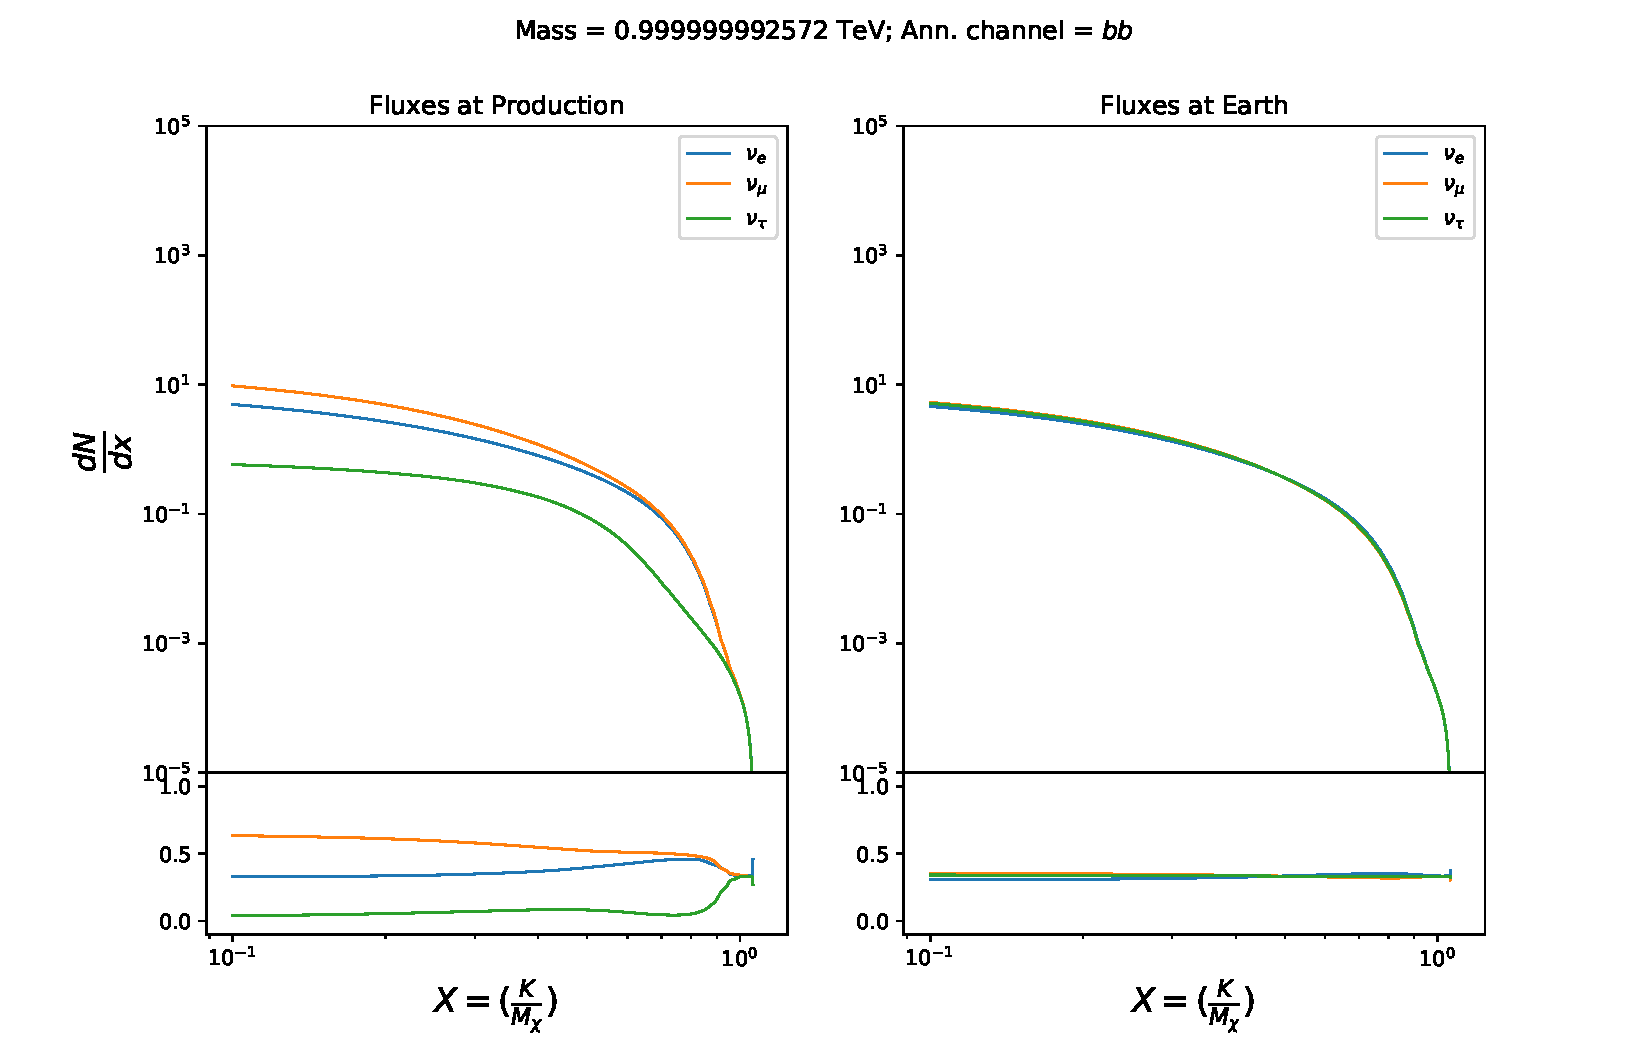
\includegraphics[scale=0.275]{figures/ic_DM/nu_spectra_bb_1.0000TeV.pdf}} &
        \raisebox{-.5\height}{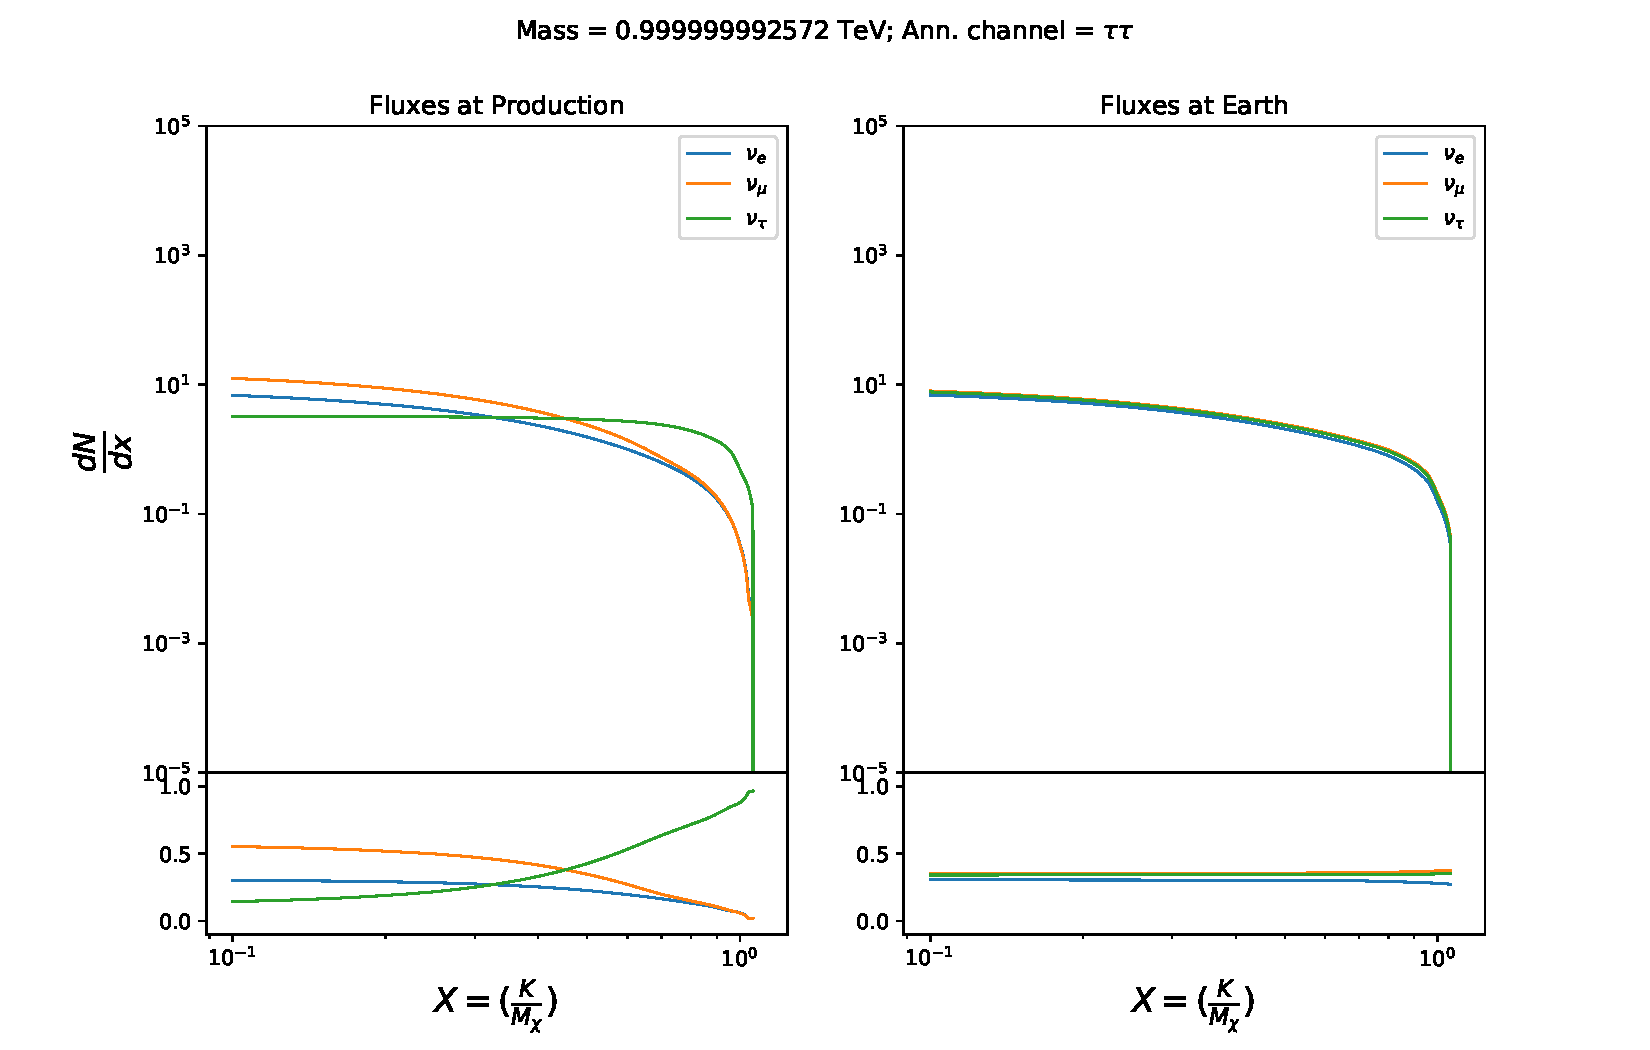
\includegraphics[scale=0.275]{figures/ic_DM/nu_spectra_tautau_1.0000TeV.pdf}} &
        \raisebox{-.5\height}{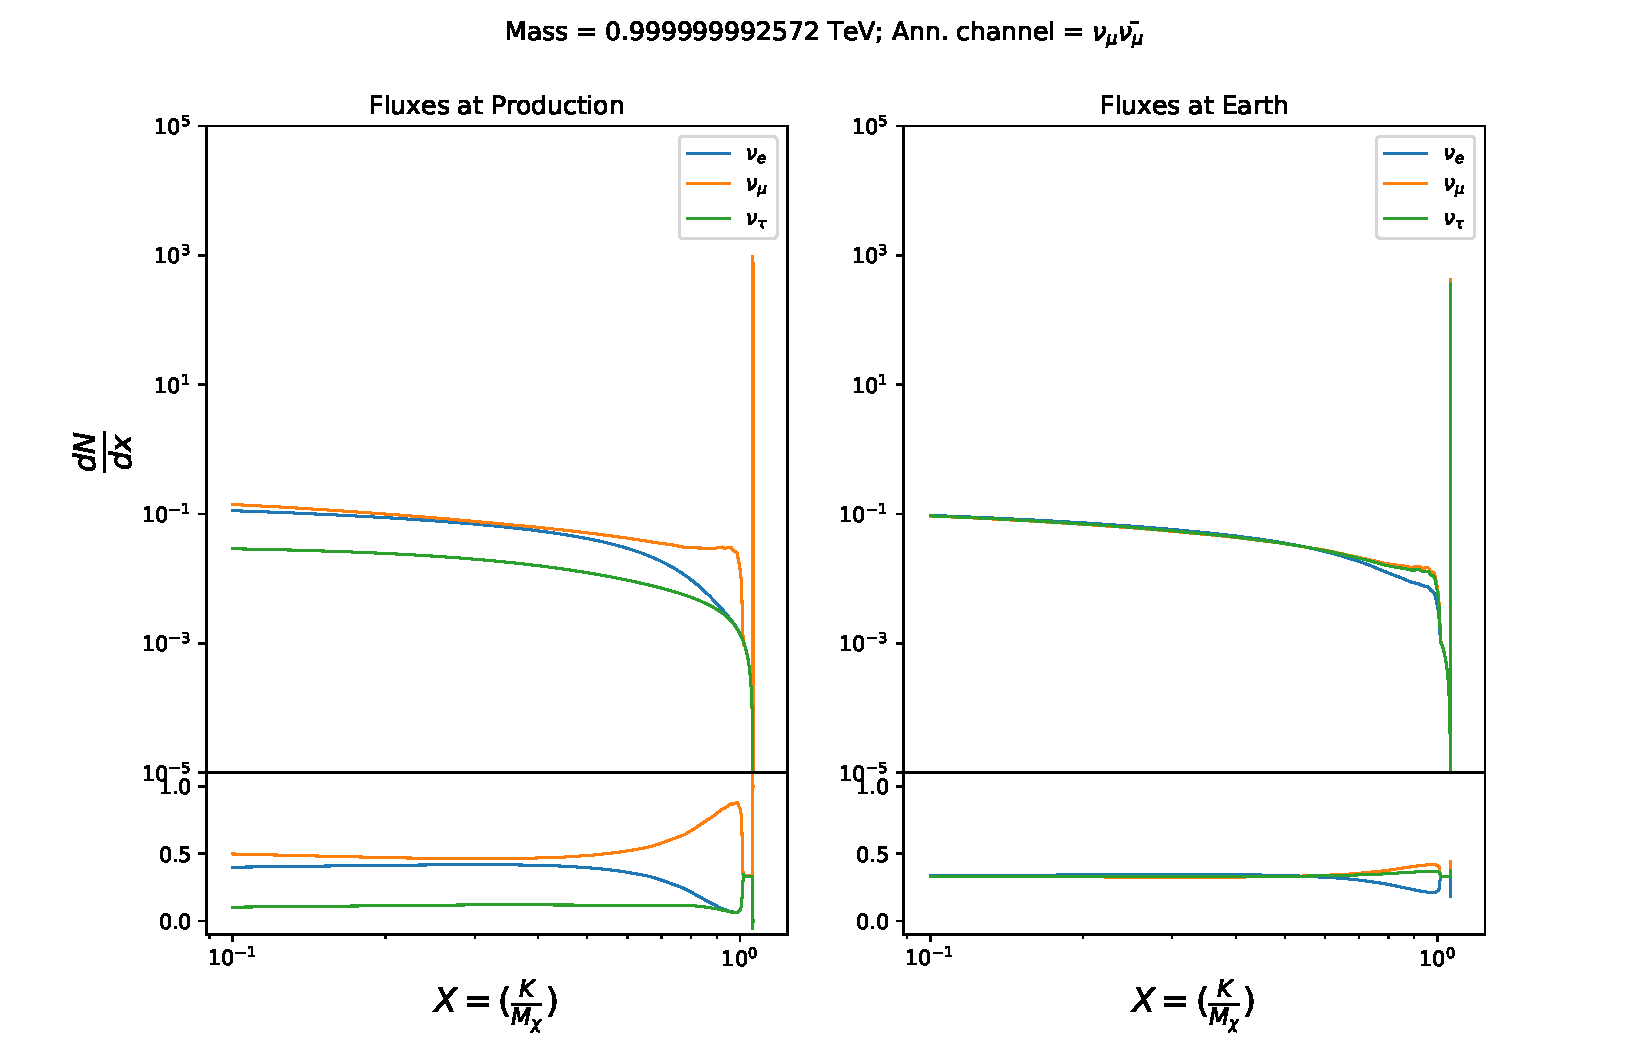
\includegraphics[scale=0.275]{figures/ic_DM/nu_spectra_numunumu_1.0000TeV.pdf}} \\

        \rotatebox[origin=c]{90}{1 PeV} &
        \raisebox{-.5\height}{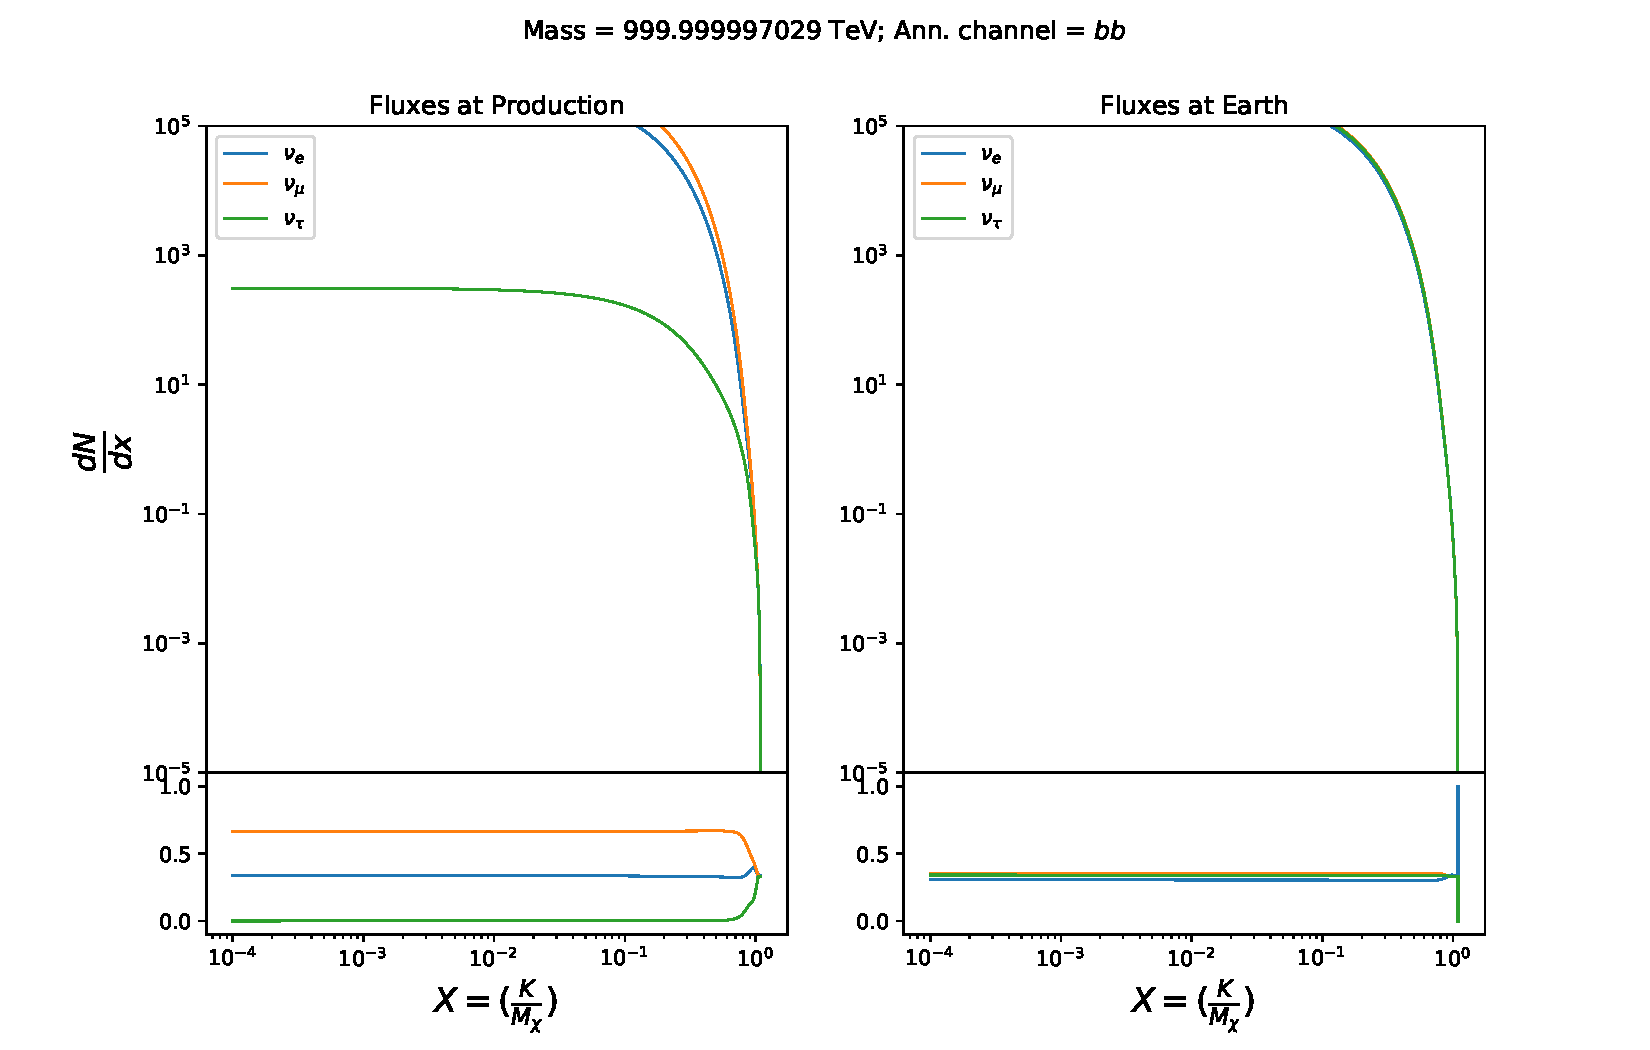
\includegraphics[scale=0.275]{figures/ic_DM/nu_spectra_bb_1000.0000TeV.pdf}} &
        \raisebox{-.5\height}{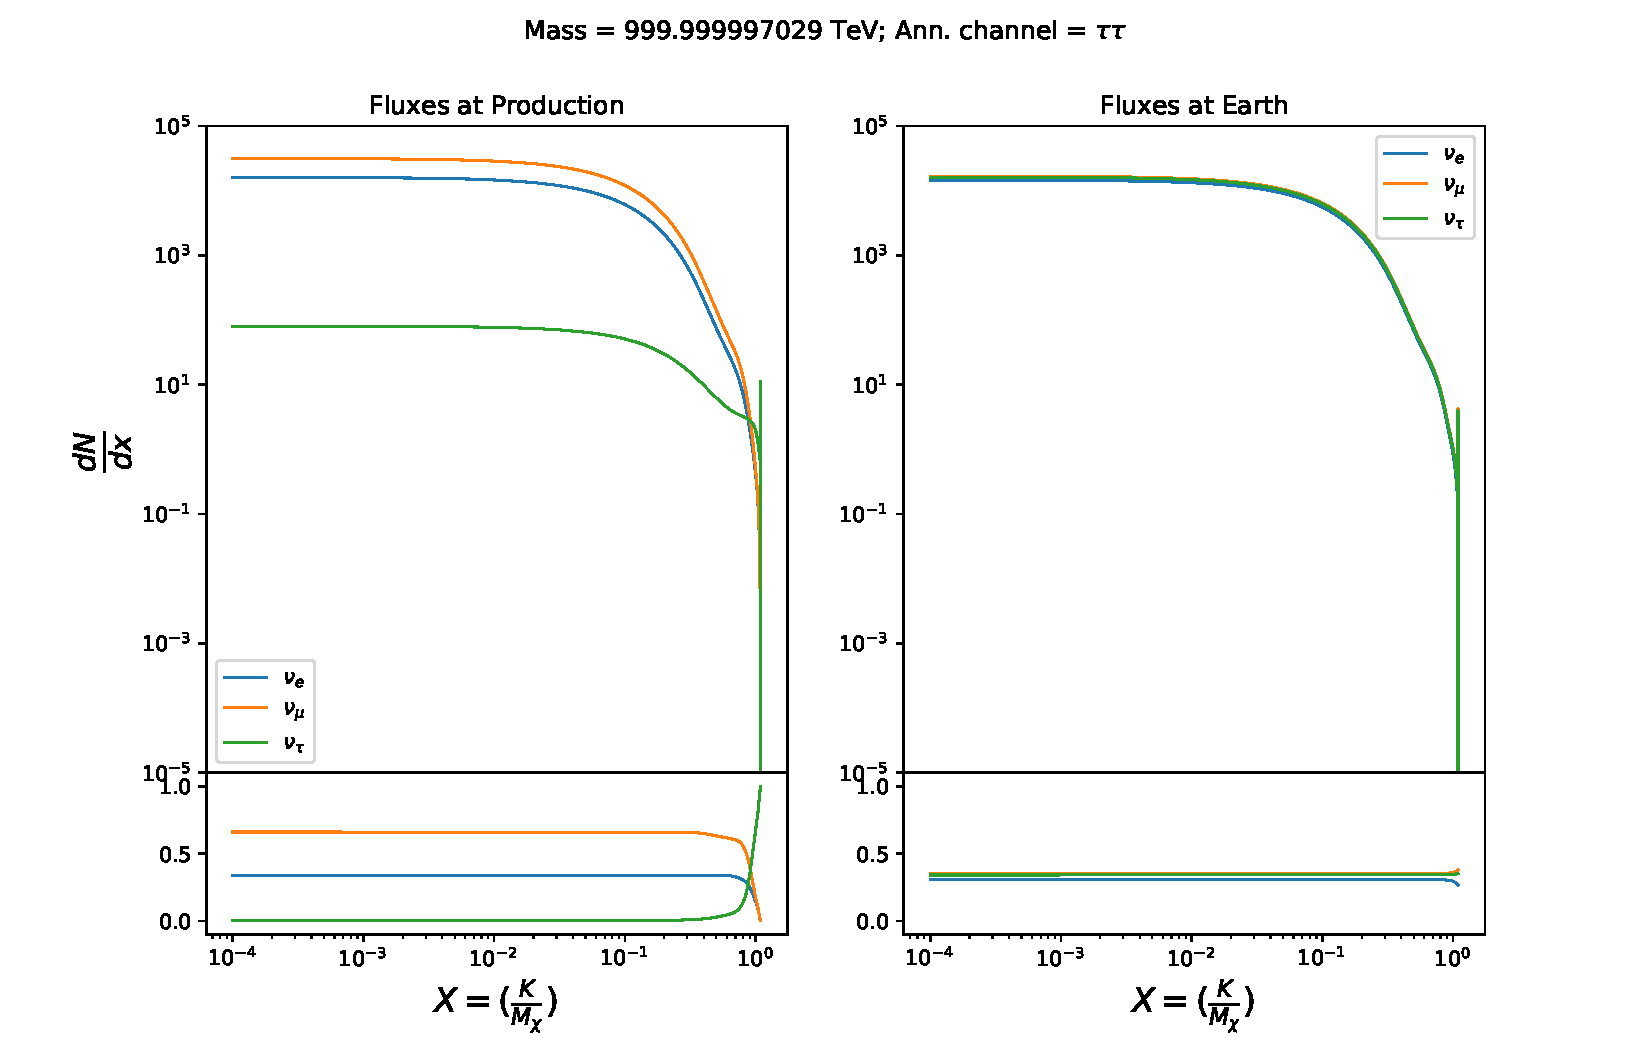
\includegraphics[scale=0.275]{figures/ic_DM/nu_spectra_tautau_1000.0000TeV.pdf}} &
        \raisebox{-.5\height}{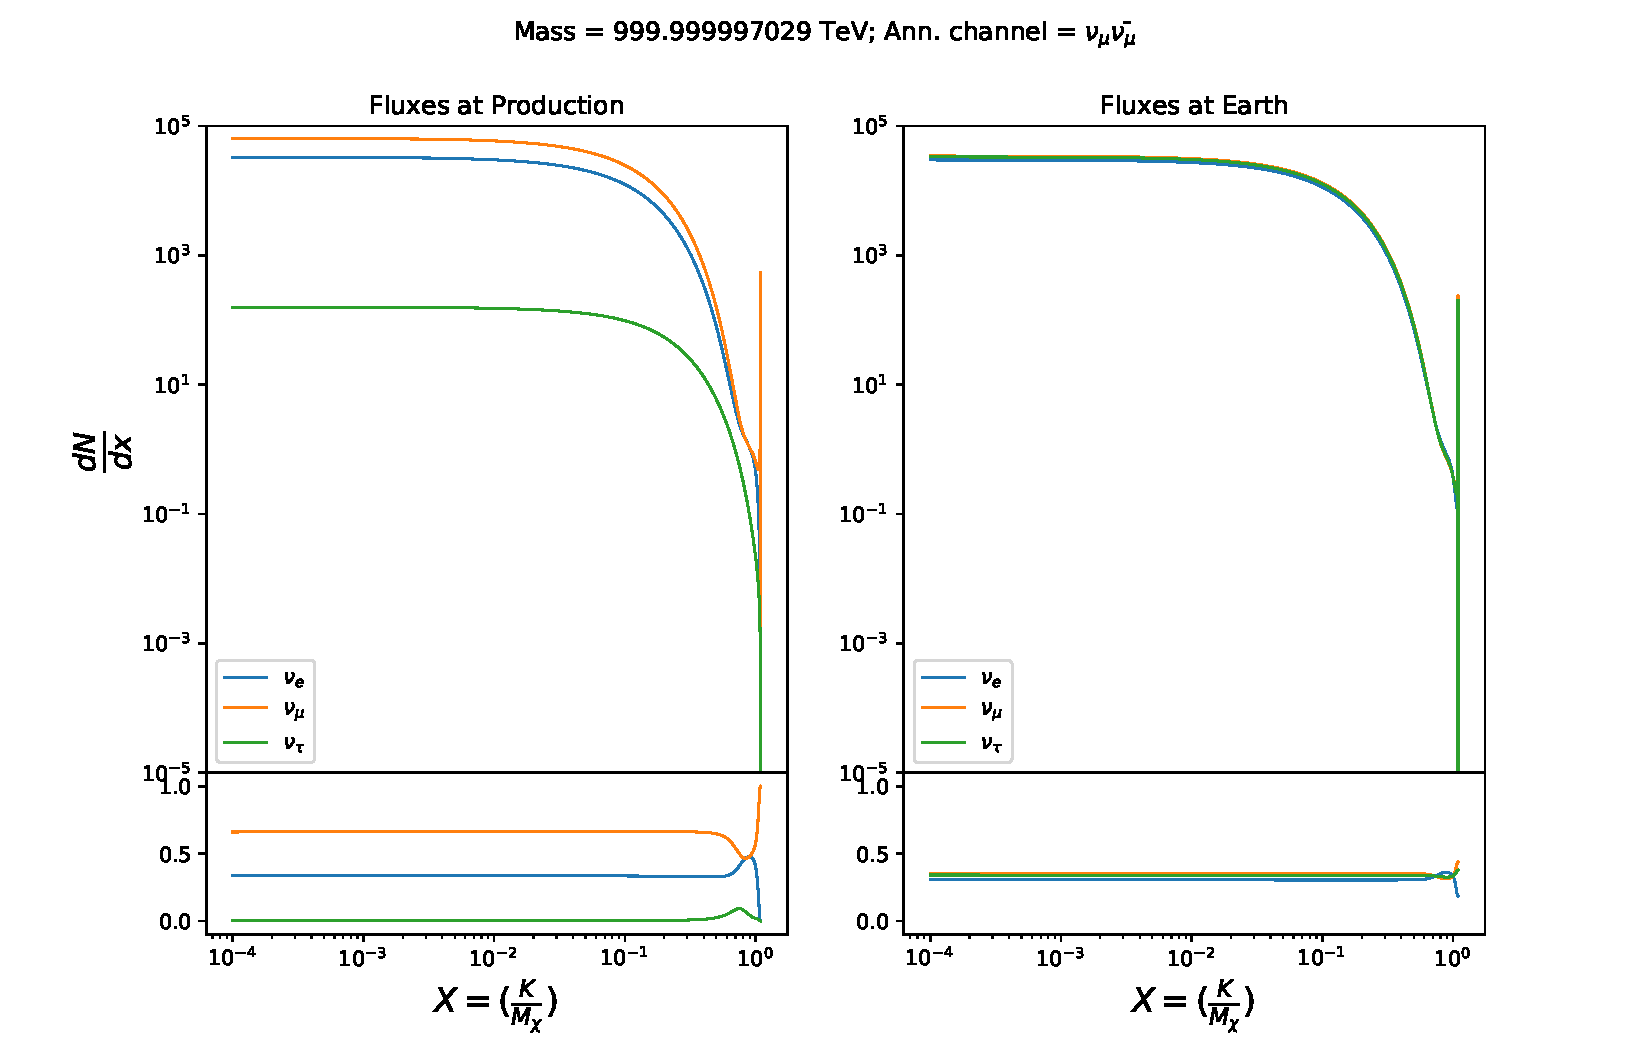
\includegraphics[scale=0.275]{figures/ic_DM/nu_spectra_numunumu_1000.0000TeV.pdf}} \\

        \rotatebox[origin=c]{90}{1 EeV} &
        \raisebox{-.5\height}{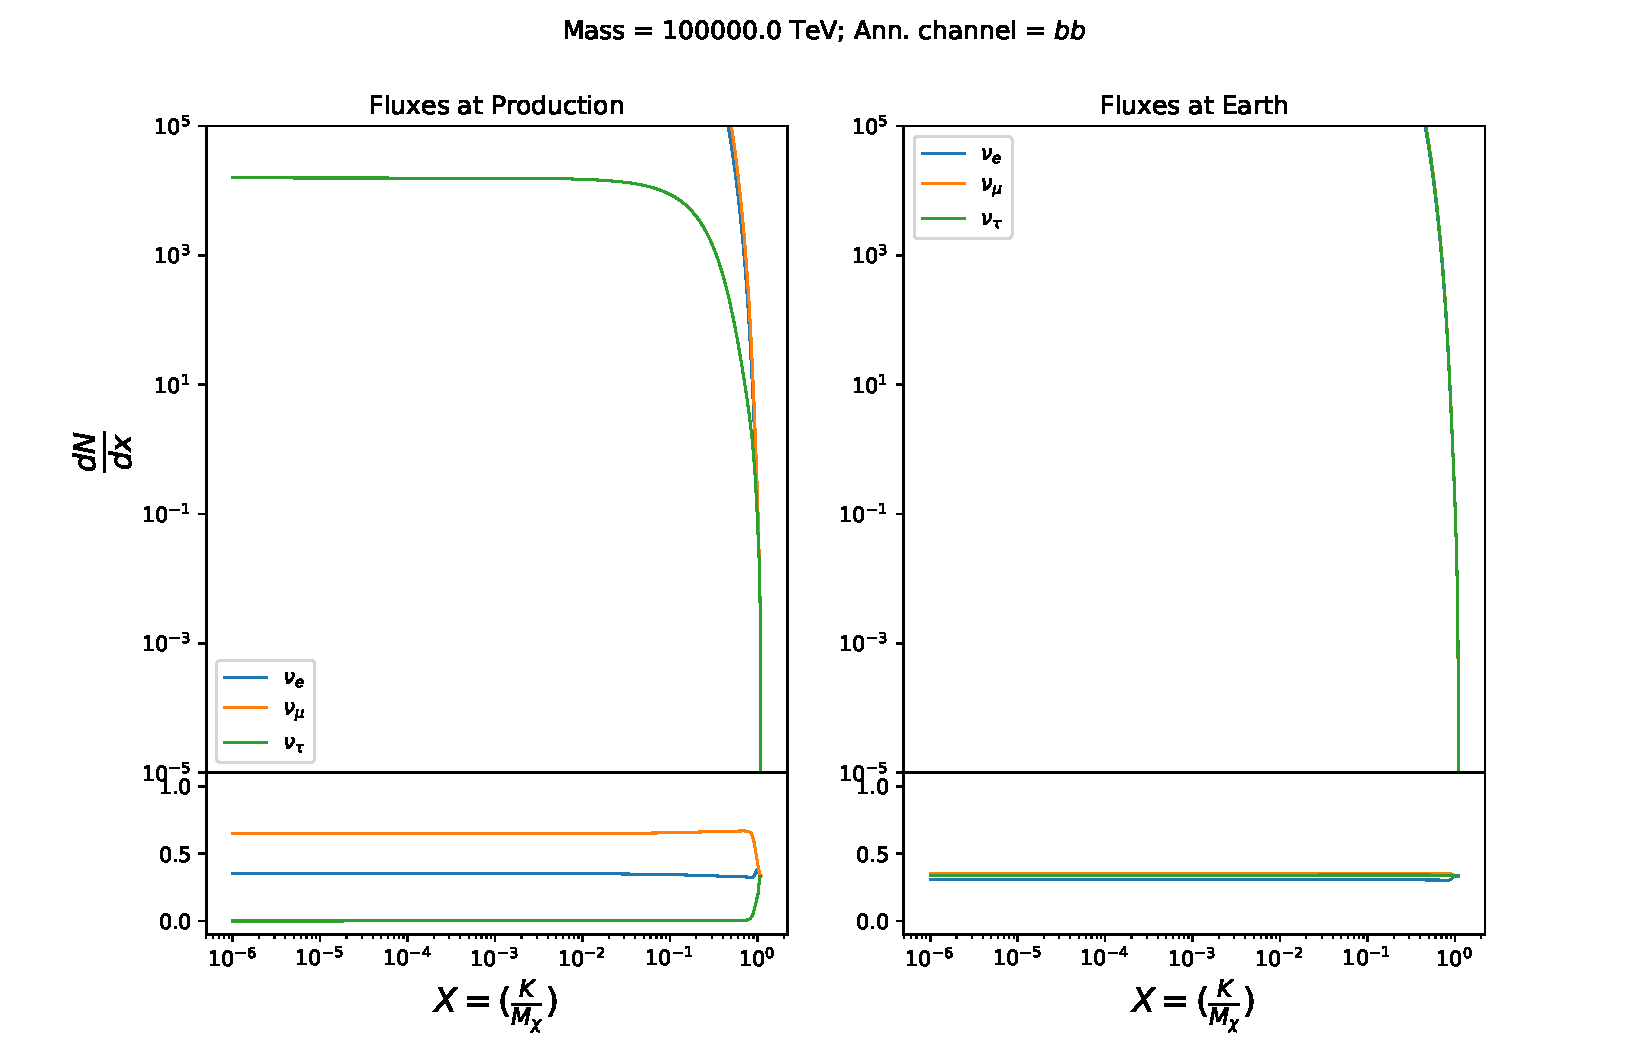
\includegraphics[scale=0.275]{figures/ic_DM/nu_spectra_bb_100000.0000TeV.pdf}} &
        \raisebox{-.5\height}{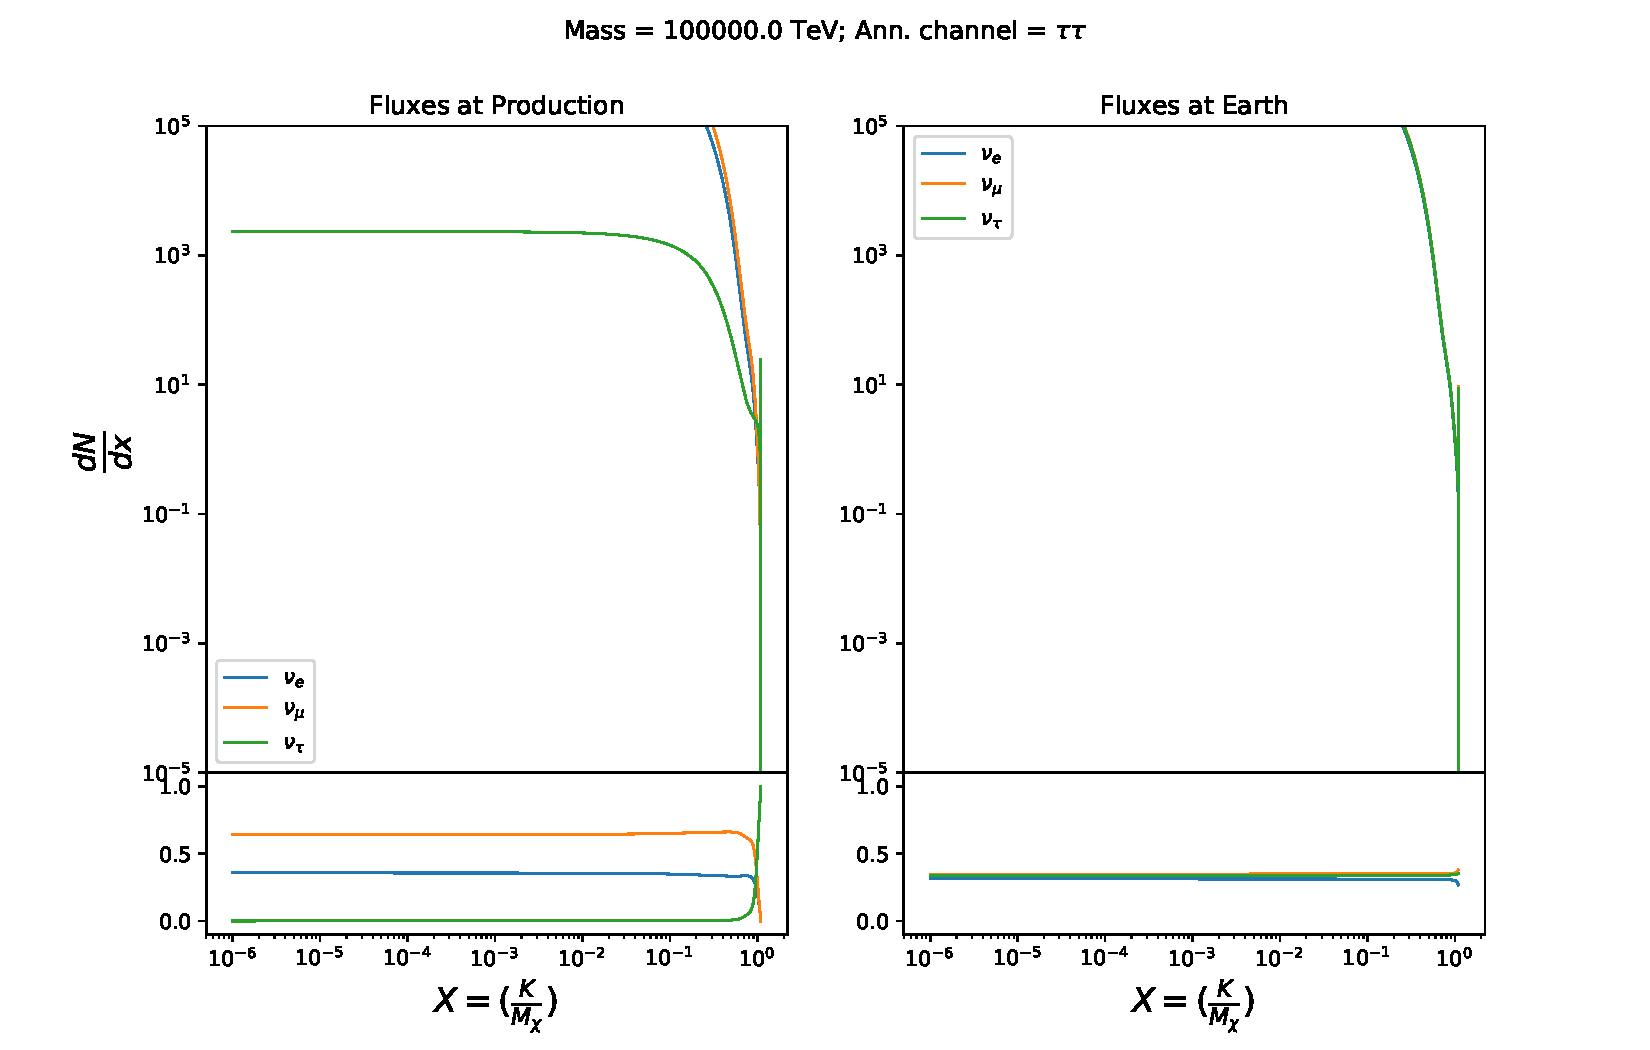
\includegraphics[scale=0.275]{figures/ic_DM/nu_spectra_tautau_100000.0000TeV.pdf}} &
        \raisebox{-.5\height}{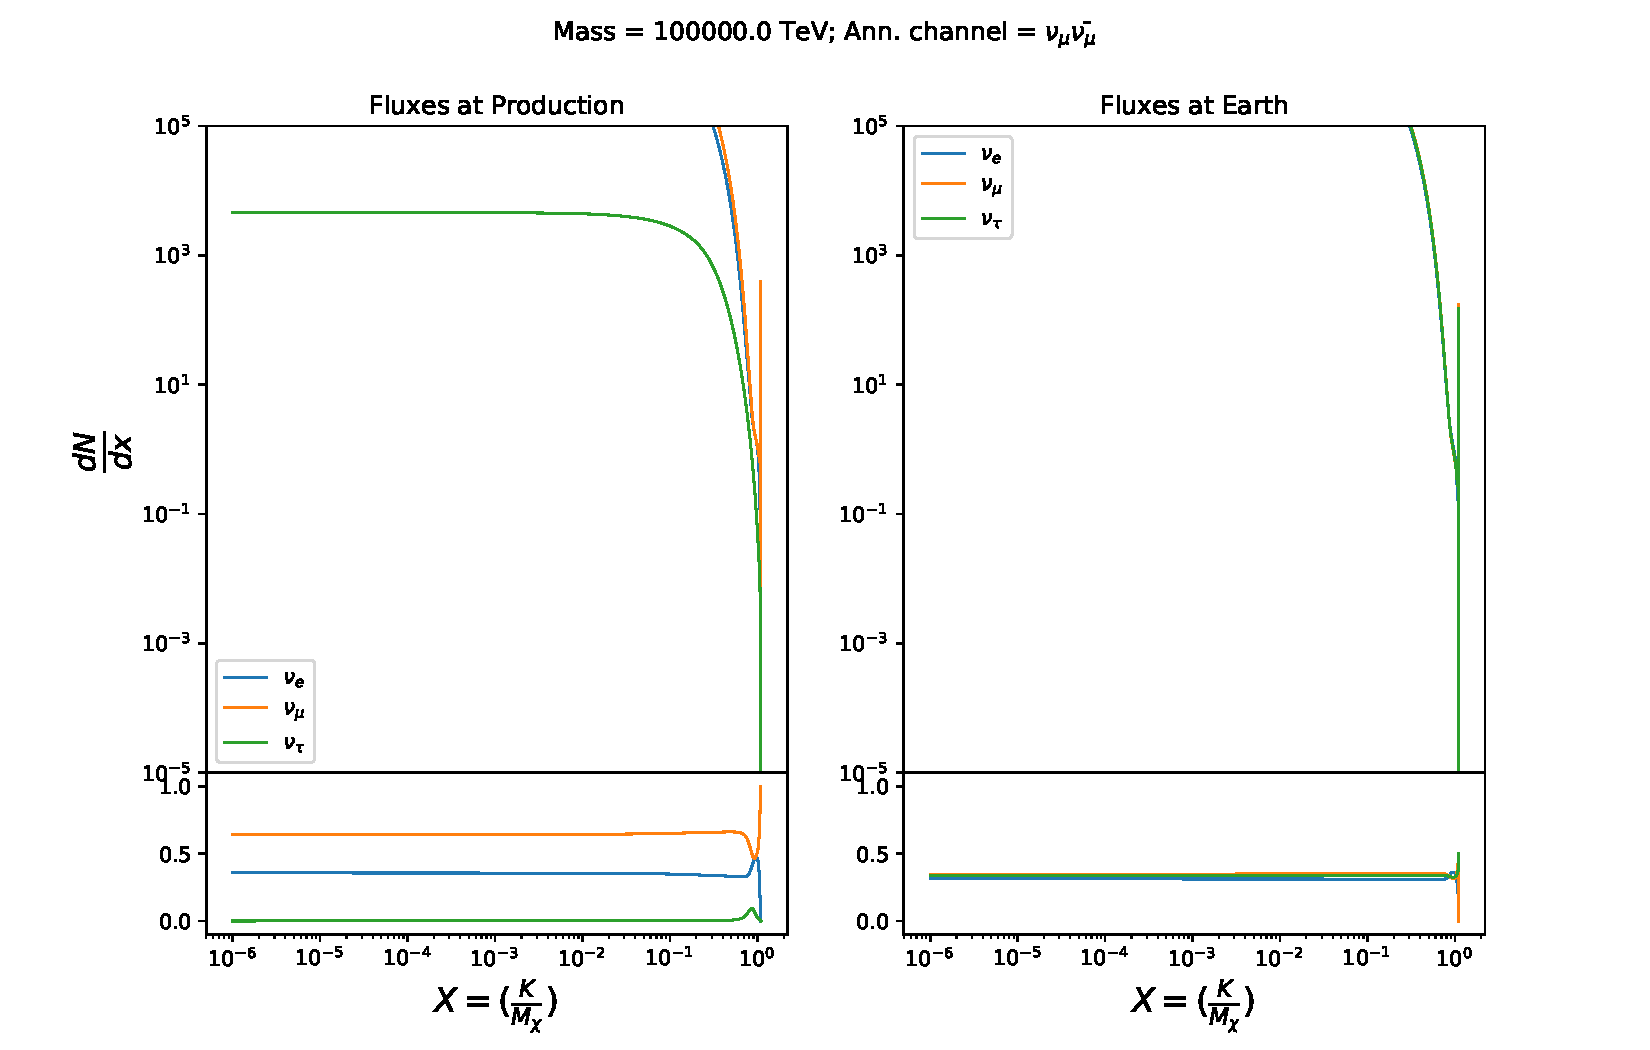
\includegraphics[scale=0.275]{figures/ic_DM/nu_spectra_numunumu_100000.0000TeV.pdf}} \\
    \end{tabular}
    \caption{Neutrino spectra at production (left panels) and after oscillation at Earth (right panels). Blue, orange, and green lines are the $\nu_e$, $\nu_\mu$, and $\nu_\tau$ spectra respectively. Top panels show the spectra in $\frac{dN}{dE}$. Lower panels plot the flavor ratio to $\nu_e + \nu_\mu + \nu_\tau$. SM annihilation channels \parpar{b}, \parpar{\tau}, and \parpar{\nu_\mu} are shown for $M_\chi =$ 1 Pev, TeV, and EeV.}
    \end{table}\label{fig:nu_osc_dm}
}
\end{landscape}
}

%%%%%%%%%%%%%%%%%%%%%%%%%%%%%%%%%%%%%%%%%%%%%%%%%%
\subsubsection{Treatment of Neutrino Line Features}\label{sec:icDM_nu_lines}
%%%%%%%%%%%%%%%%%%%%%%%%%%%%%%%%%%%%%%%%%%%%%%%%%%

All DM annihilation channels into leptons $ \chi\chi \rightarrow [\nu_{e, \mu, \tau}, e, \mu,\tau] $ develop a prominent and narrow spectral line feature.
For all neutrino flavors, this line is visible and prominent in all $m_\chi$ studied in this anlysis.
For charged leptons, the feature only really shows up at the larger DM mass models and varies between the flavors.
Examples for lines in the annihilation spectra with neutrinos or charged leptons primary annihilation products are provided in \cref{fig:icDM_osc_dm}.

The neutrino line feature is so narrow relative the sampled energy range that the random sampling of the spectra and likelihood fitting rarely capture the line in computation.
As a result, often the best fit to simulation of background will always floor to TS = 0 and the signal recovery systematically underestimates the signal (see \cref{fig:sig_recovery_fail}).

\begin{figure}[t]
    \centering{
        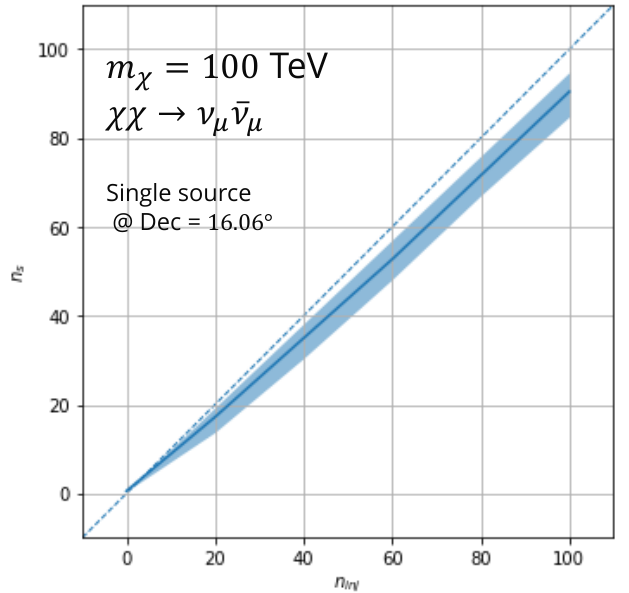
\includegraphics[scale=0.5]{figures/ic_DM/Sig_recover_line.png}
    }
    \caption{Signal recovery for 100 TeV DM annihilation into \parpar{\nu_\mu} for a source at Dec = 16.06$^\circ$. $n_\mathrm{inj}$ is the number of injected signal events in simulation. $n_s$ is the number of reconstructed signal events from the simulation. Although the uncertainties are small and tight, the reconstructed $ n_s $ are systematically underestimated.} \label{fig:sig_recovery_fail}
\end{figure}

To remedy this, a similar approach to the IceCube's decay analysis \cite{Minjin_icrc23}.
Two smoothing kernels were tested (Gaussian, uniform) to widen the line feature.
The widths were tuned such that the signal recovery approached unity for DM mass 100 TeV to 1 PeV for a source at Segue 1's declination, $16.06^\circ$.
Near horizon was chosen in order to isolate loss in signal recovery from too narrow a line versus from Earth's attenuation of very high energy neutrinos.
The convolution also needed to as close as possible preserve the integrated counts of neutrinos.
The optimized kernel window for all lines is summarized as:
\begin{itemize}
    \item Guassian kernel with $2 \sigma$ width = 3.5E-3$\cdot m_\chi$
    \item Minimum energy included in convolution = MIN$[0.995 \cdot m_\chi, E(\nu_\mathrm{line}) -4\sigma]$
    \item Maximum energy included in convolution = MAX$[1.005 \cdot m_\chi, E(\nu_\mathrm{line}) +4\sigma]$
\end{itemize}
where $E(\nu_{\mathrm{line}})$ is the neutrino energy where the neutrino line is at the maximum.

\begin{figure}[h]
    \centering{

    \begin{tabular}{cc}
        \begin{tabular}{cc}
            \rotatebox[origin=c]{90}{\small{$\frac{dN}{dX}$}} &
            \raisebox{-.5\height}{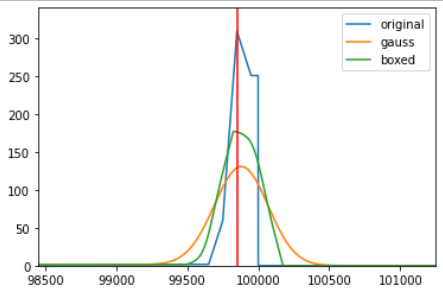
\includegraphics[scale=0.5]{figures/ic_DM/sig_recovery_fixed copy.png}} \\

            &
            \small{$E_\nu$ (GeV)} \\
        \end{tabular} &

        \raisebox{-.5\height}{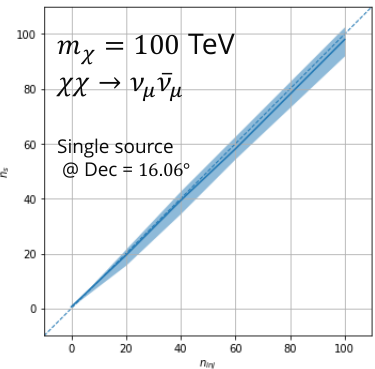
\includegraphics[scale=0.5]{figures/ic_DM/sig_recovery_fixed.png}} \\
    \end{tabular}
    }\caption{Left panel shows the two kernels overlaying the original spectrum from $\chi$aron$\nu$ after propagation to Earth \cite{Charon}. The vertical red line indicates where the original neutrino line is maximized. Blue line is the output from $\chi$aro$\nu$. Green line is the spectrum after convolution with a flat kernel. Orange line is the spectrum after Gaussian convolution. Right panel shows the signal recovery of the spectral model using the Gaussian kernel with parameters enumerated above.} \label{fig:icDM_fixed_line}
\end{figure}

These parameters broadly improved the signal recovery of the line spectra.
An example is in \cref{fig:icDM_fixed_line}.
Signal recovery studies for are expanded upon in \cref{sec:icDM_sig_recovery}.

%%%%%%%%%%%%%%%%%%%%%%%%%%%%%%%%%%%%%%%%%%%%%%%%%%
\subsubsection{Spline Fitting}\label{sec:icDM_splines}
%%%%%%%%%%%%%%%%%%%%%%%%%%%%%%%%%%%%%%%%%%%%%%%%%%

In an effort to reduce computational work, memory burden, and align with point source methods used for NGC1068 \cite{IC_NGC1068}, spectral splines were created and adopted for estimating the neutrino flux for the different spectral models.
Software was written to generate, book keep, and calculate values on the splines.

When using splines, one has to be careful of the goodness to fit.
The spline software used here, Photospline \cite{photospline}, uses the penalized spline technique.
Through the penlized technique, poor fits are penalized according to the accuracy of the nominal value, and the smoothness of the first and second derivatives.
The B-spline construction however does not penalize on the integral of the fit distrubtion which is critical in low signal studies, such as DM searches.
There are additional caveats when testing the goodness to fit to the MC generated above for all DM annihilation channels.
\begin{itemize}
    \item The splines must be Log10(*) in Energy and dN/dE to account for the exponential nature of the flux.
    \item The fidelity of the fit matters more at $ E_\nu \thickapprox m_\chi $ where the model uncertainties are minimal and physical considerations (like the cut-off) are most important.
    \item The fidelity of the fit matters less at low $ E_\nu $ as the model uncertainties are large AND IceCube's sensitivity diminishes significantly below 500 GeV.
    \item Total integrated counts should be well preserved.
\end{itemize}
The resulting cost function was built to evaluate the goodness of spline fits to account for the above considerations.
\erriSpline
Where $ \hat{e_i} $ is the spline estimator's value for $x_i$. $ x_i = E_{\nu_i} / m_\chi $. $ \frac{dN_i}{dE_i} $ is the flux value from MC.
I then take the RMS of the error distribution and the resulting value, err, is used to evaluate the fidelity of the spectral spline.
\MSEspline

Each SM channel had unique tolerances for 'err'.
Channels with very hard cut-offs had looser tolerance for err because a significant error would be generated from single counts over/underestimated at the cut-off.
Soft channels do not share this issue, so the tolerance is much stricter.
All annihilation channels from HDM are modeled well below IceCube's NST sensitivity.
We do not think it is necessary to evaluate the spline fits below 100 GeV \cite{IC3_thesis_Cerver} and use this value as the default lower cut-off.
Yet, HDM's model uncertainties at $E_\nu < 10^{-6}\cdot m_\chi$ span an order of magnitude \cite{HDMSpectra}.
We also choose not to evaluate the splines below this critical value if it is within IceCube's sensitivity.
Finally, the smoothing of the spectral lines in leptonic annihilation channels are ignored for evaluating the fit.
We used the lower limit of the kernel mask as the upper limit of evaluation.
\Cref{tab:spline_tolerance} summarizes the tolerances for the DM annihilation channels used for this analysis.
\begin{table}
    \centering{
    \begin{tabular}{c|c c c c}
        \hline
        $ \chi\chi \rightarrow $ &
        GOOD &
        OK   &
        FAIL &
        Limits of err calc [$X_{min}, X_{max}$] \\
        \hline
        \hline

        $ Z^0Z^0, W^+W^- $ &
        $1.0 \cdot 10^{-3}$ &
        \makecell{$1.0 \cdot 10^{-3}$, \\ $1.0 \cdot 10^{-2}$} &
        $1.0 \cdot 10^{-2}$ &
        MAX$[100 \mathrm{GeV}/m_\chi, 10^{-6}], 1.0 $ \\
        \hdashline

        $ t\bar{t}, hh $ &
        $1.0 \cdot 10^{-5}$ &
        \makecell{$1.0 \cdot 10^{-5}$, \\ $1.0 \cdot 10^{-4}$} &
        $1.0 \cdot 10^{-4}$ &
        MAX$[100 \mathrm{GeV}/m_\chi, 10^{-6}], 1.0 $ \\
        \hdashline

        $ b\bar{b}, d\bar{d}, u\bar{u}$ &
        $9.0 \cdot 10^{-7}$ &
        \makecell{ $9.0\cdot 10^{-7}$, \\ $9.0 \cdot 10^{-6}$} &
        $9.0 \cdot 10^{-6}$ &
        MAX$[100 \mathrm{GeV}/m_\chi, 10^{-6}], 1.0 $ \\
        \hdashline

        $ \nu\bar{\nu}_{e, \mu, \tau} $ &
        $1.0 \cdot 10^{-3}$ &
        \makecell{$1.0 \cdot 10^{-3}$, \\ $1.0 \cdot 10^{-2}$} &
        $1.0 \cdot 10^{-2}$ &
        \makecell{MAX$[100 \mathrm{GeV}/m_\chi, 10^{-6}]$, \\ MIN$[0.995, (E_{\nu_{line}}) -4\sigma)/M_{\chi}] $} \\
        \hdashline

        $ e\bar{e}, \mu\bar{\mu}, \tau\bar{\tau} $ &
        $1.0 \cdot 10^{-3}$ &
        \makecell{$1.0 \cdot 10^{-3}$, \\ $1.0 \cdot 10^{-2}$}&
        $1.0 \cdot 10^{-2}$ &
        \makecell{MAX$[100 \mathrm{GeV}/m_\chi, 10^{-6}]$, \\ MIN$[0.995, (E_{\nu_{line}}) -4\sigma)/M_{\chi}]$} \\

    \end{tabular}
    }
    \caption{Spline err tolerances used for input in particle physics component to \cref{eq:id_dm_flux}. Column 1 is the DM annihilation channel being fit. Columns 2, 3, and 4 are the tolerances for "GOOD" (pass), "OK" requires inspection, and "FAIL" (tune and refit) respectively. Column 5 has the X ranges over which the error is evaluated. MAX/MIN [$\cdot$,$\cdot$] takes the maximum or minumum of the two enclosed values.} \label{tab:spline_tolerance}
\end{table}

The errors are then plotted in two ways.
First, FAIL and OK are directly plotted with $e_i$ as a function of x, and the full spline and MC.
AN example of a single failure is provided in \cref{fig:icDM_failedspline}
Second, a summary plot of all the splines is plotted and colors coded.
\Cref{fig:apdx_nu_splines} are the spline summaries as of writing this thesis.
The goal broadly is to eliminate all red and inspect yellow statuses.

\begin{figure}
    \centering{
    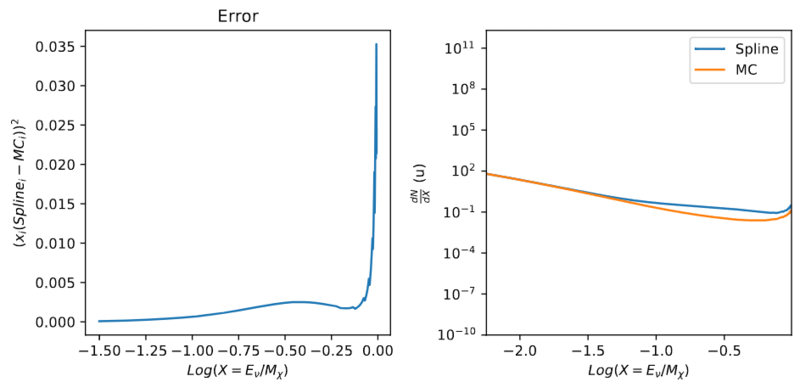
\includegraphics[scale=0.6]{figures/ic_DM/800px-Failed_spline.png}
    }
    \caption{Example spline that failed the fit. Failed splined are corrected on a case by case basis unless the SM channel has a systematic problem fitting the splines. In this case, I made a bookkeeping error and loaded the incorrect spectral model}
    \label{fig:icDM_failedspline}
\end{figure}

The $\nu_e$ spectra at Earth are not considered in this analysis, so no work was done to refine the spline fits for this flavor.
A Final inspection of the splines by eye to verify that the spline fitting did not introduce spurious features into the distribution that would corrupt the likelihood fitting.

%%%%%%%%%%%%%%%%%%%%%%%%%%%%%%%%%%%%%%%%%%%%%%%%
\subsubsection{Composite Neutrino Spectra}\label{sec:icDM_composite_dNdE}
%%%%%%%%%%%%%%%%%%%%%%%%%%%%%%%%%%%%%%%%%%%%%%%

With all of the previously mentioned pieces, we are ready to fully assemble a comprehensive description of the particle physics term $dN/dE$ in \cref{eq:id_dm_flux}.
\nuIDDMFlux

\begin{figure}[t]
    \centering{
        \begin{tabular}{ccc}
            $\chi\chi \rightarrow$ \parpar{e} &
            $\chi\chi \rightarrow$ \parpar{\mu} &
            $\chi\chi \rightarrow$ \parpar{\tau} \\

            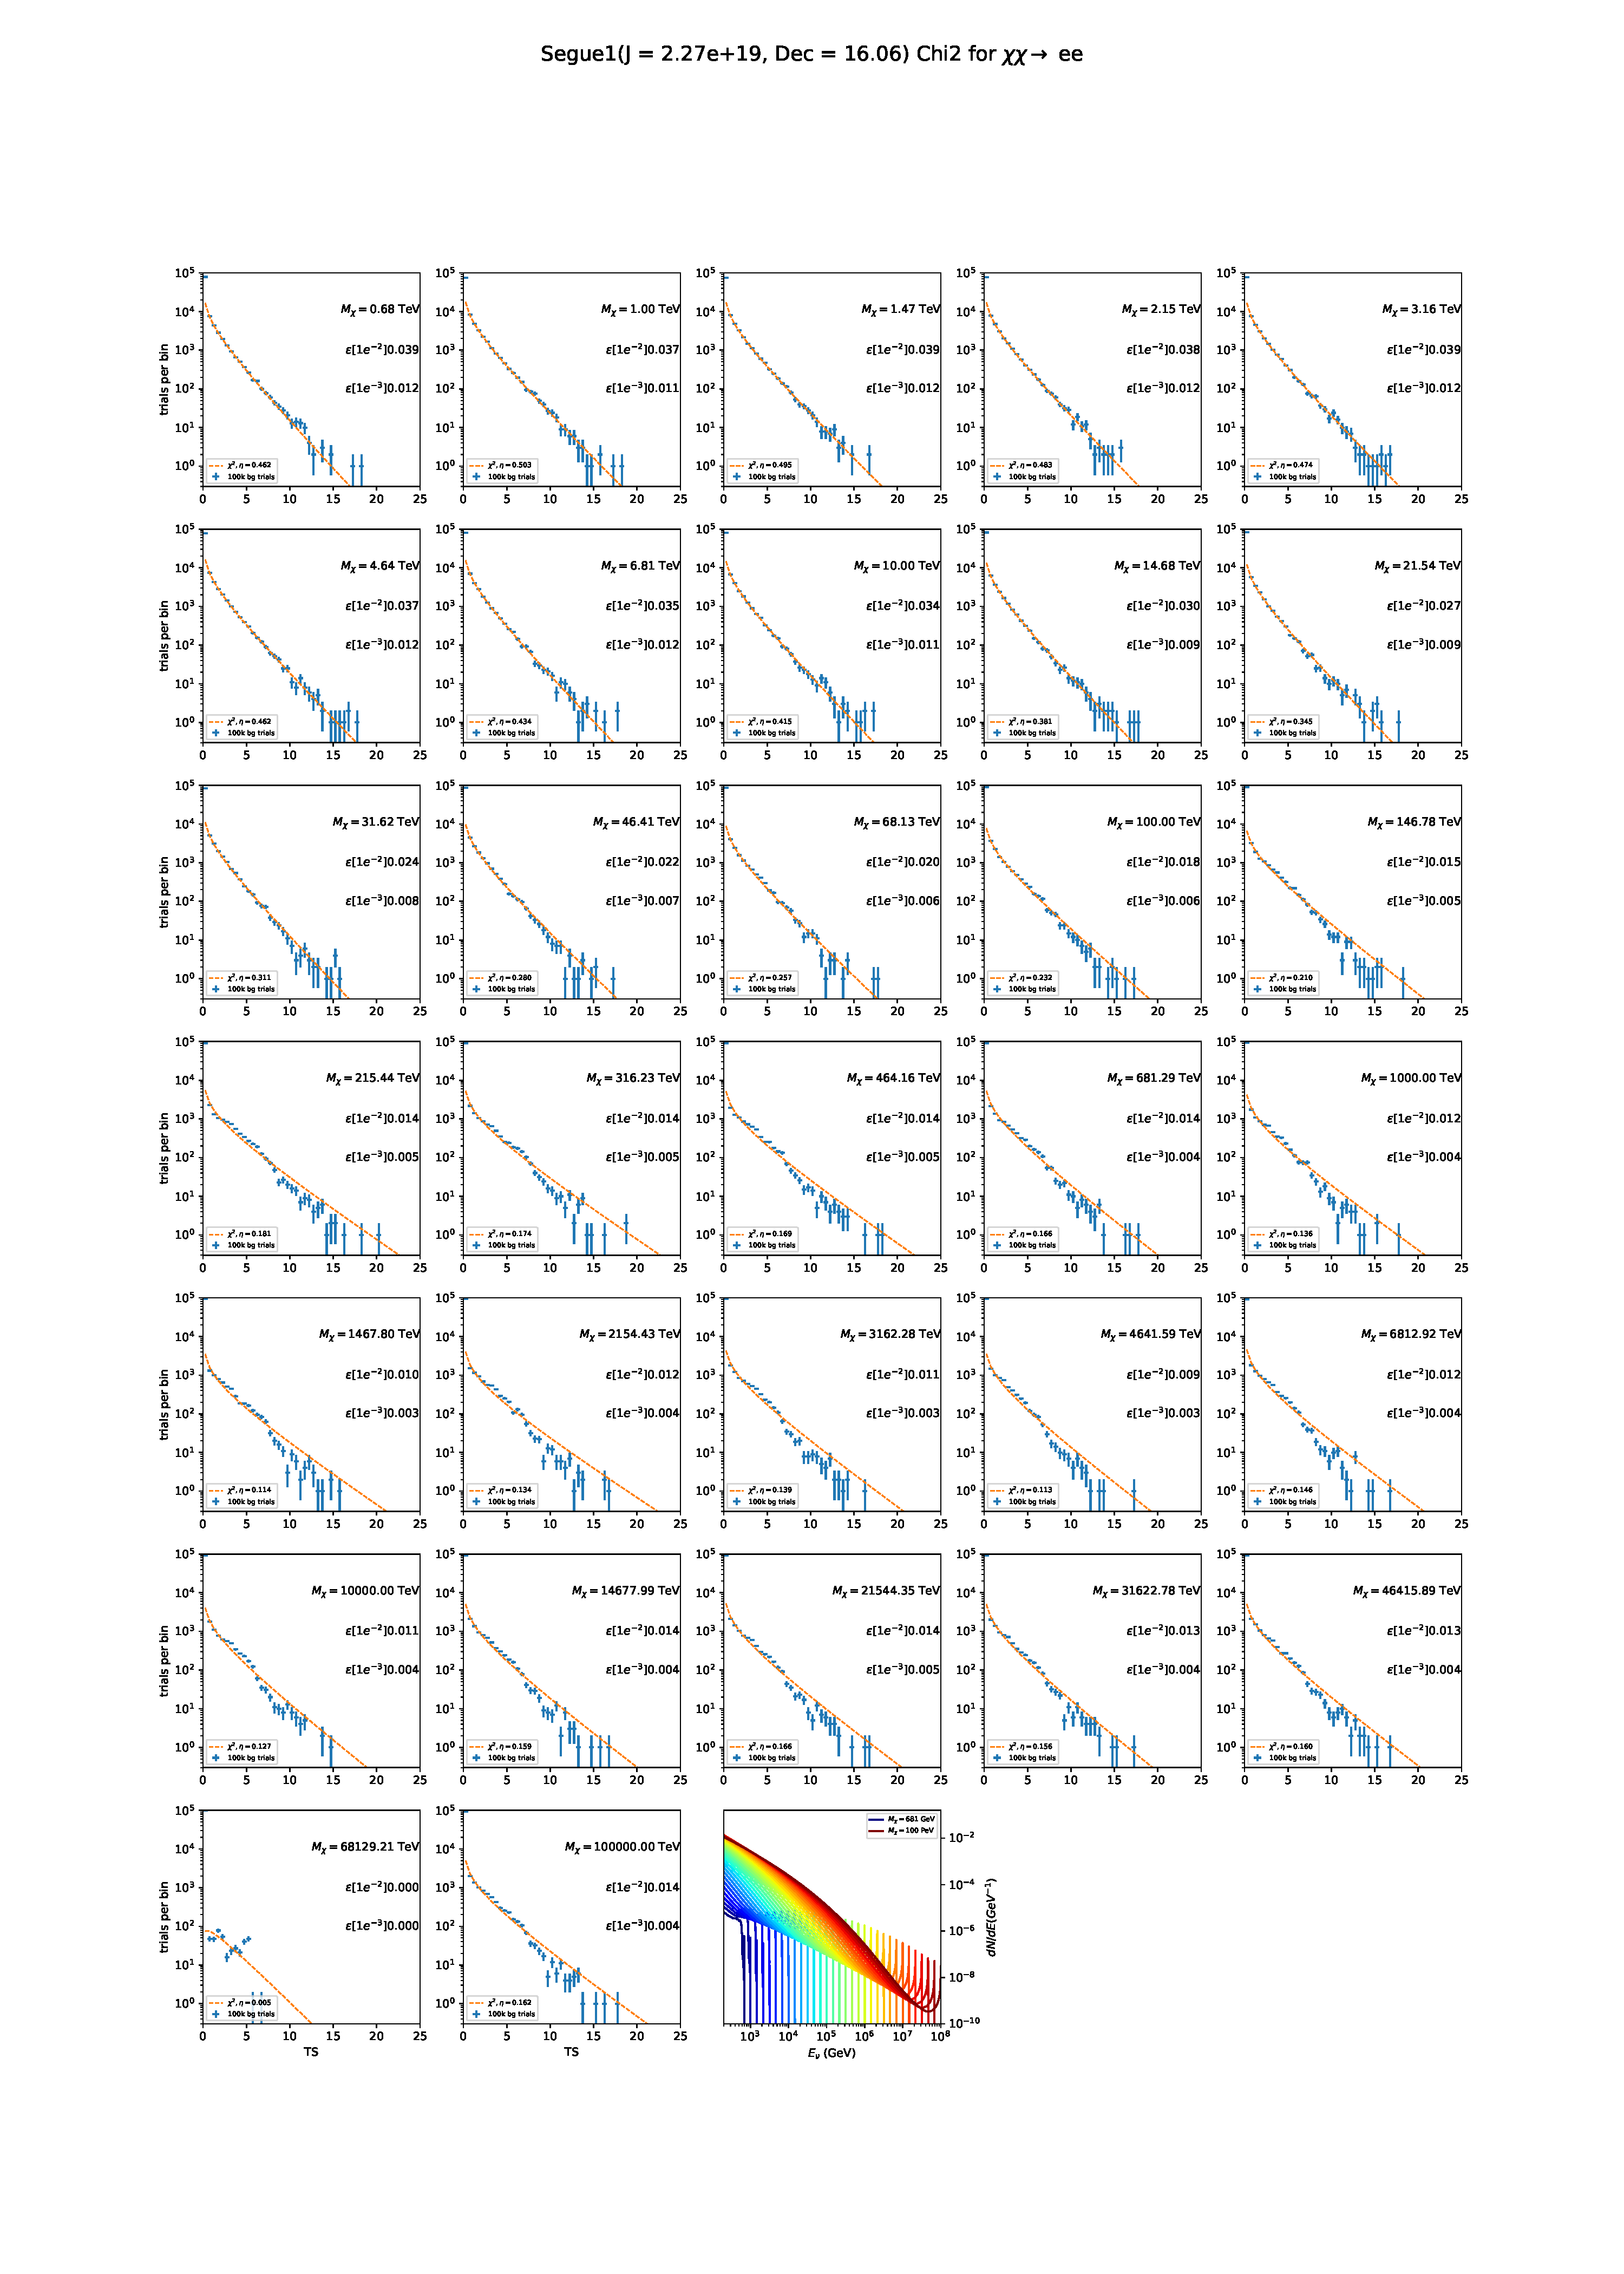
\includegraphics[clip, trim=22.1cm 6.5cm 19.5cm 56.5cm, scale=0.55]{figures/ic_DM/dm_plots/Segue1_ee_chi2_Masspanel_2024-03-23.pdf} &
            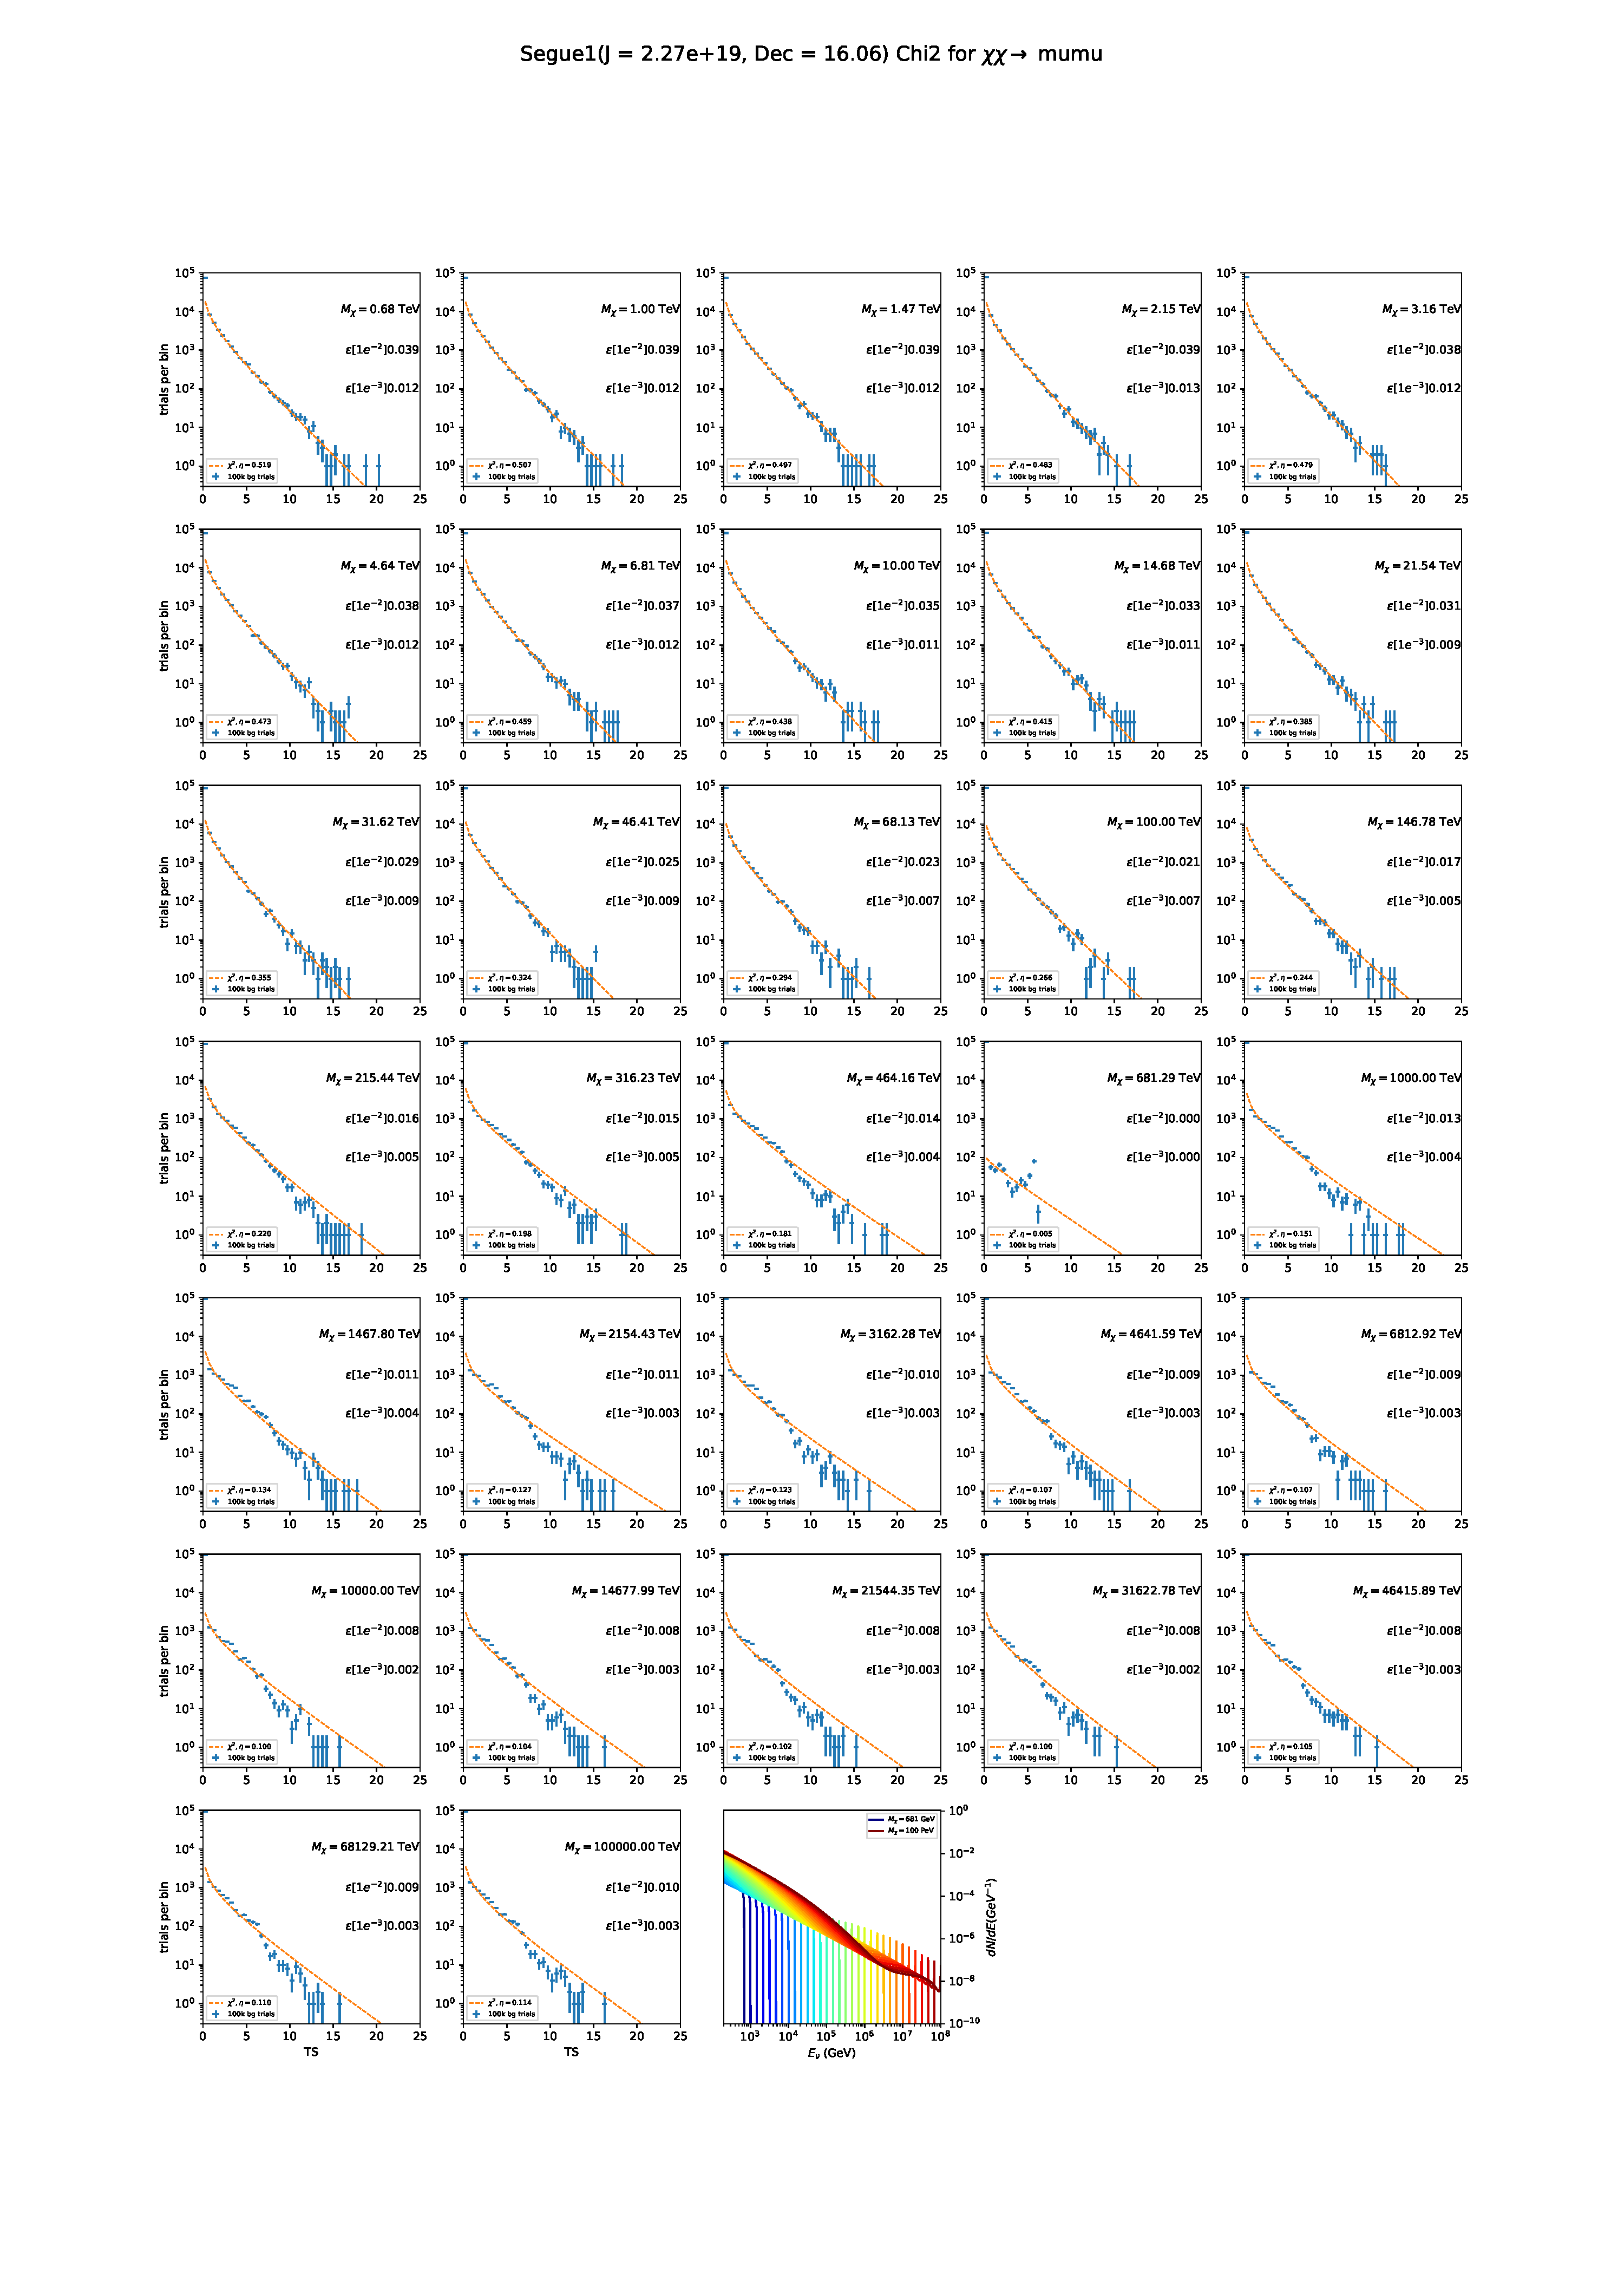
\includegraphics[clip, trim=22.1cm 6.5cm 19.5cm 56.5cm, scale=0.55]{figures/ic_DM/dm_plots/Segue1_mumu_chi2_Masspanel_2024-03-23.pdf} &
            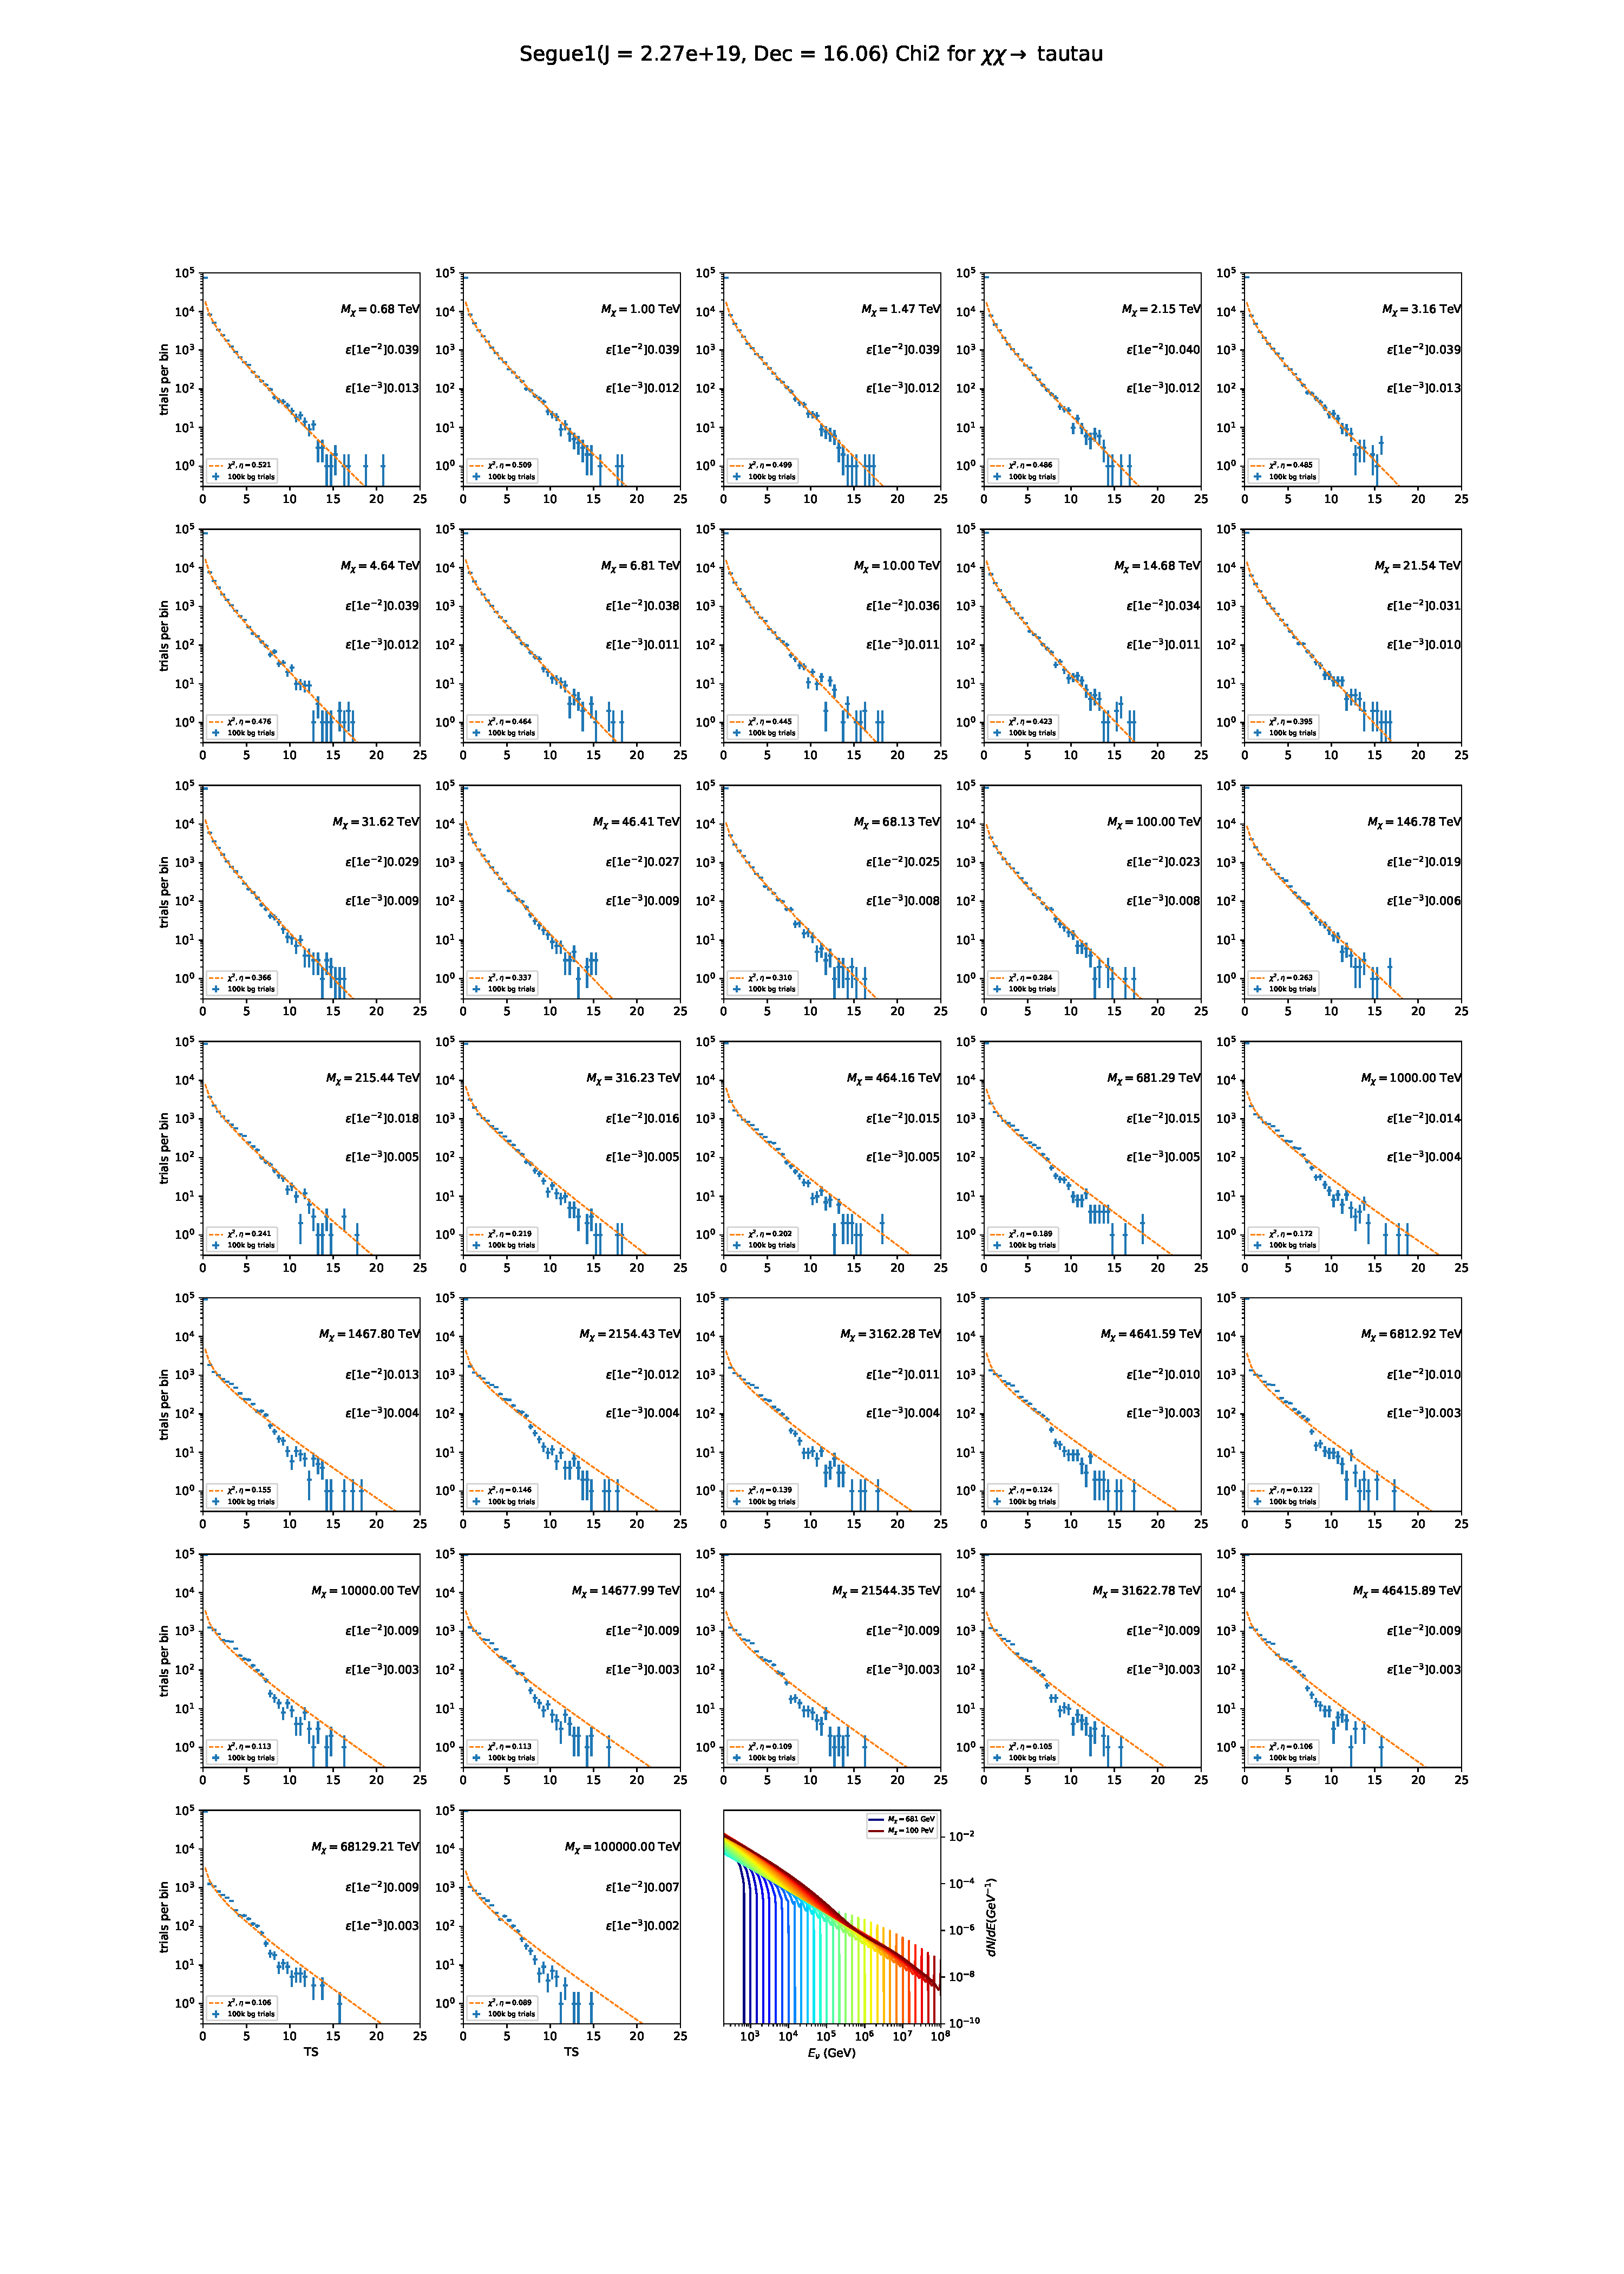
\includegraphics[clip, trim=22.1cm 6.5cm 19.5cm 56.5cm, scale=0.55]{figures/ic_DM/dm_plots/Segue1_tautau_chi2_Masspanel_2024-03-23.pdf} \\


            $\chi\chi \rightarrow$ \parpar{\nu_e} &
            $\chi\chi \rightarrow$ \parpar{\nu_\mu} &
            $\chi\chi \rightarrow$ \parpar{\nu_\tau} \\

            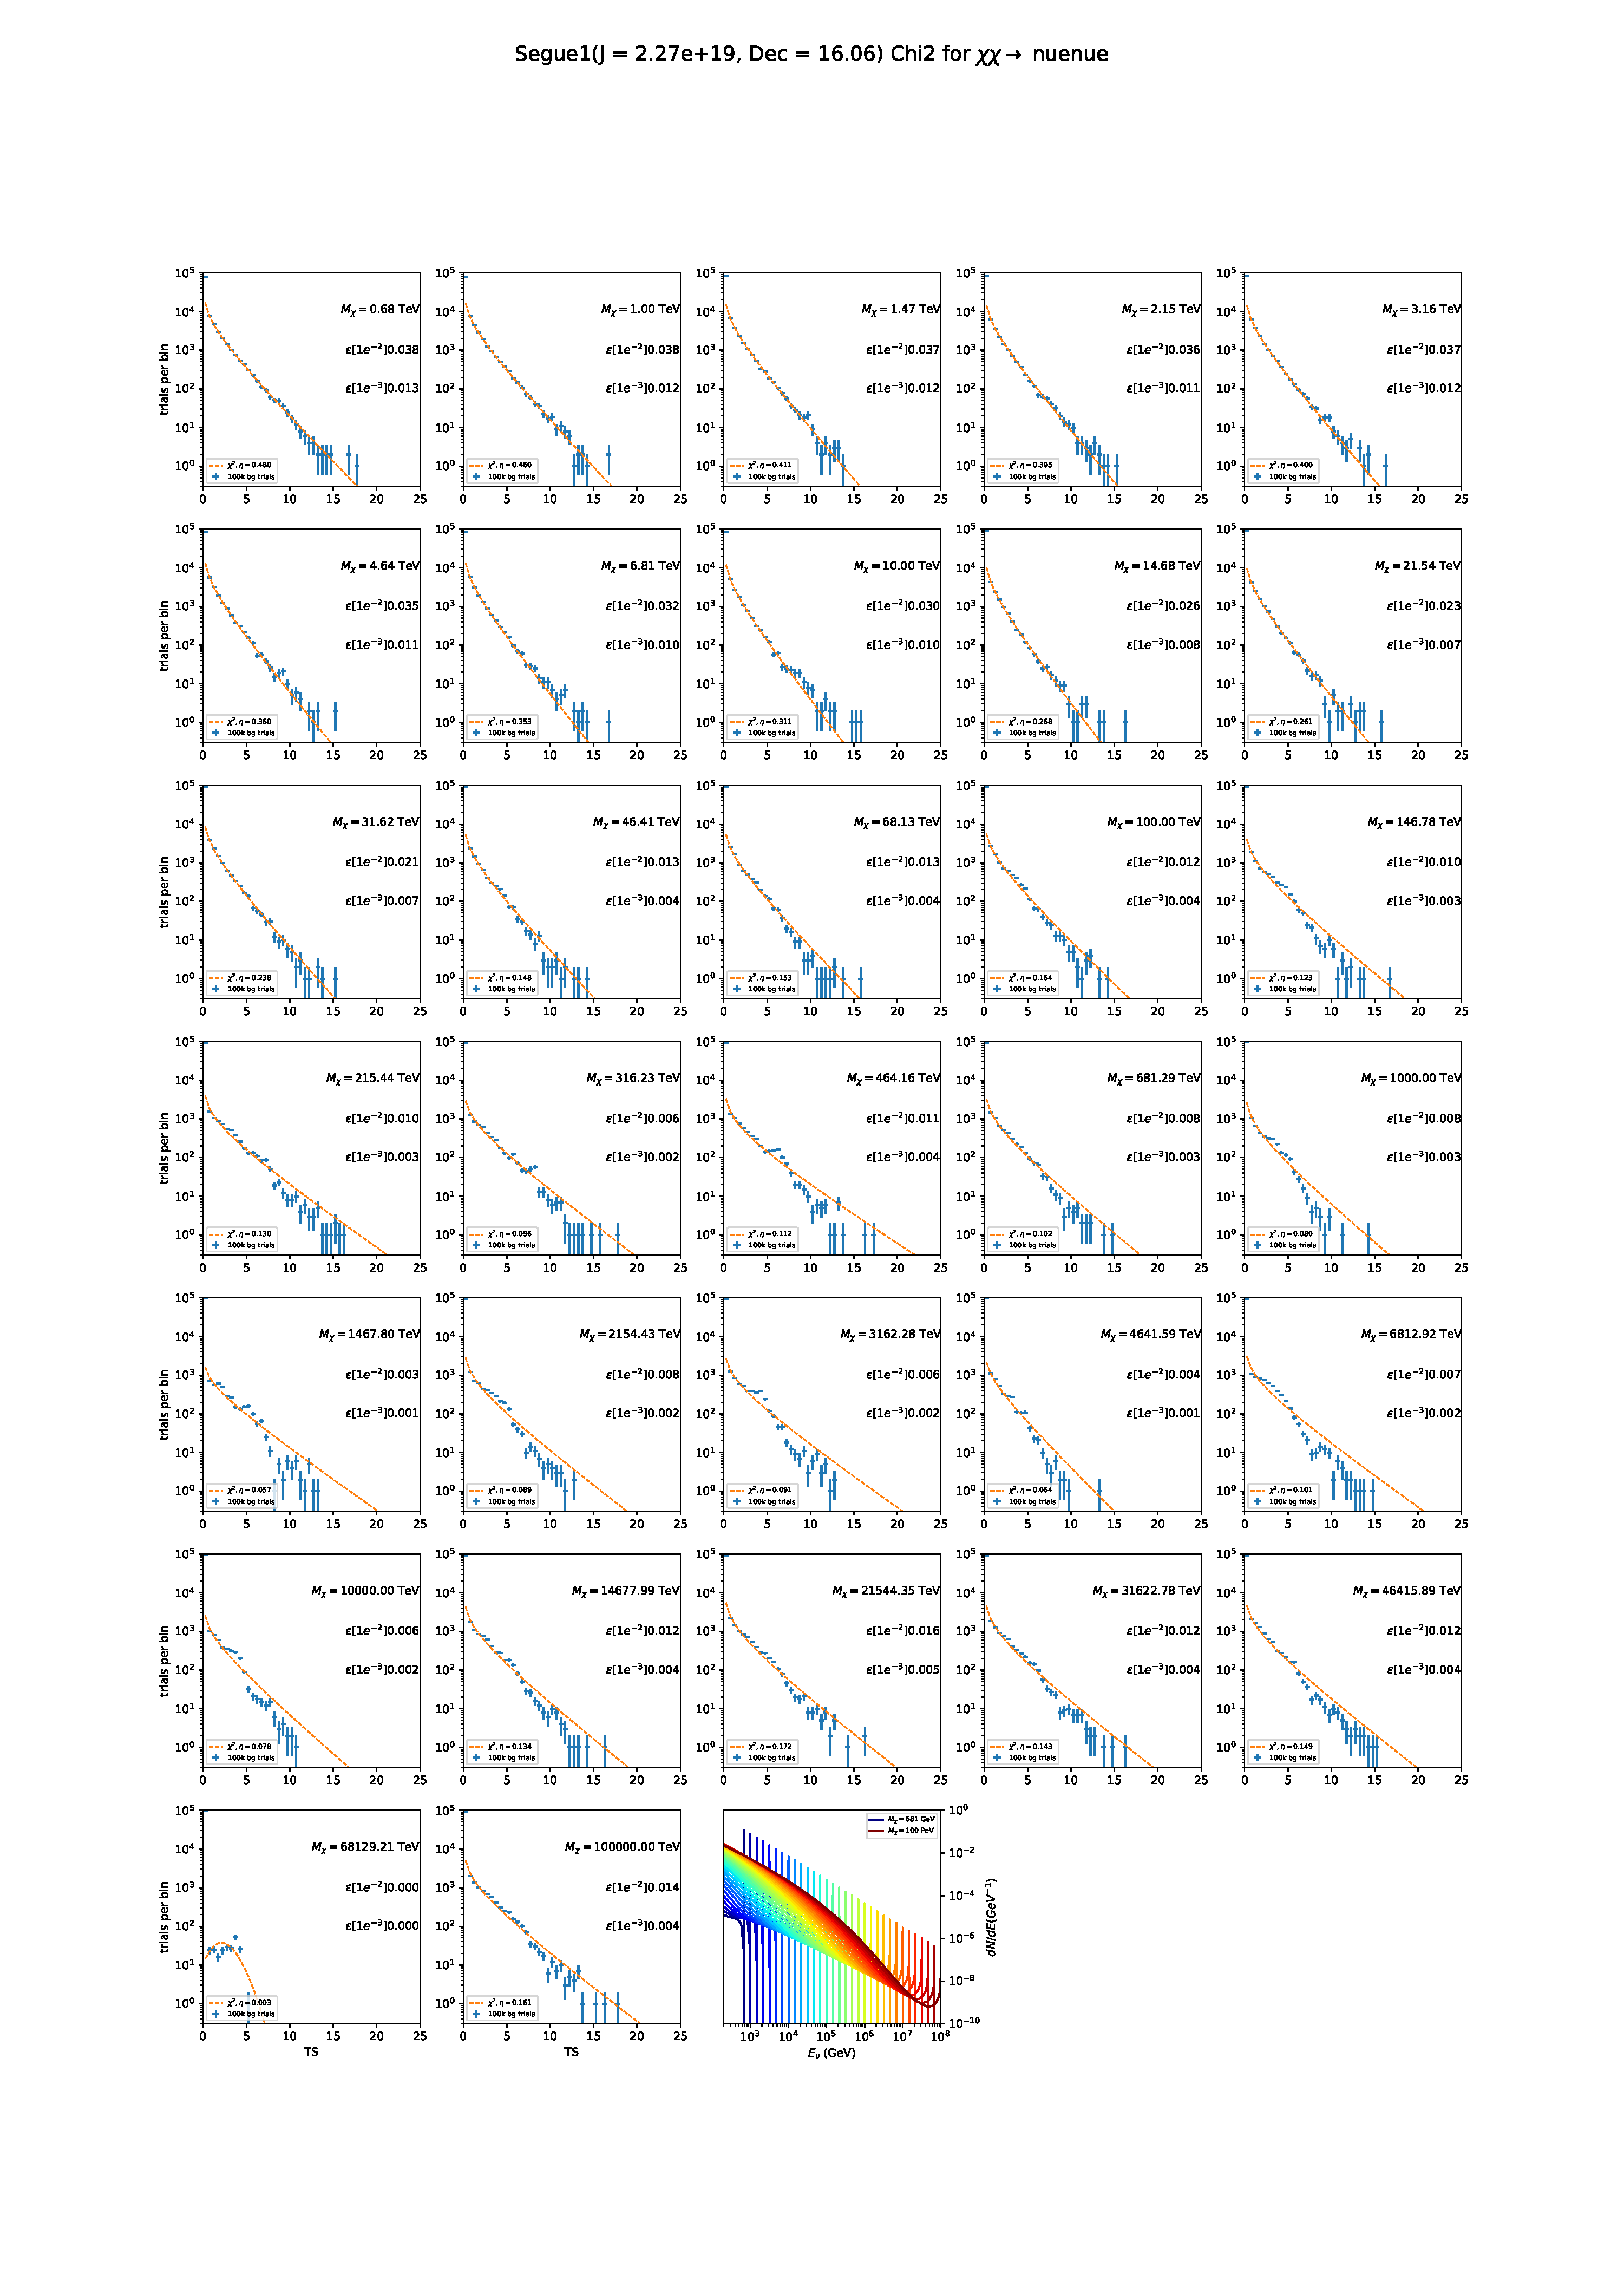
\includegraphics[clip, trim=22.1cm 6.5cm 19.5cm 56.5cm, scale=0.55]{figures/ic_DM/dm_plots/Segue1_nuenue_chi2_Masspanel_2024-03-23.pdf} &
            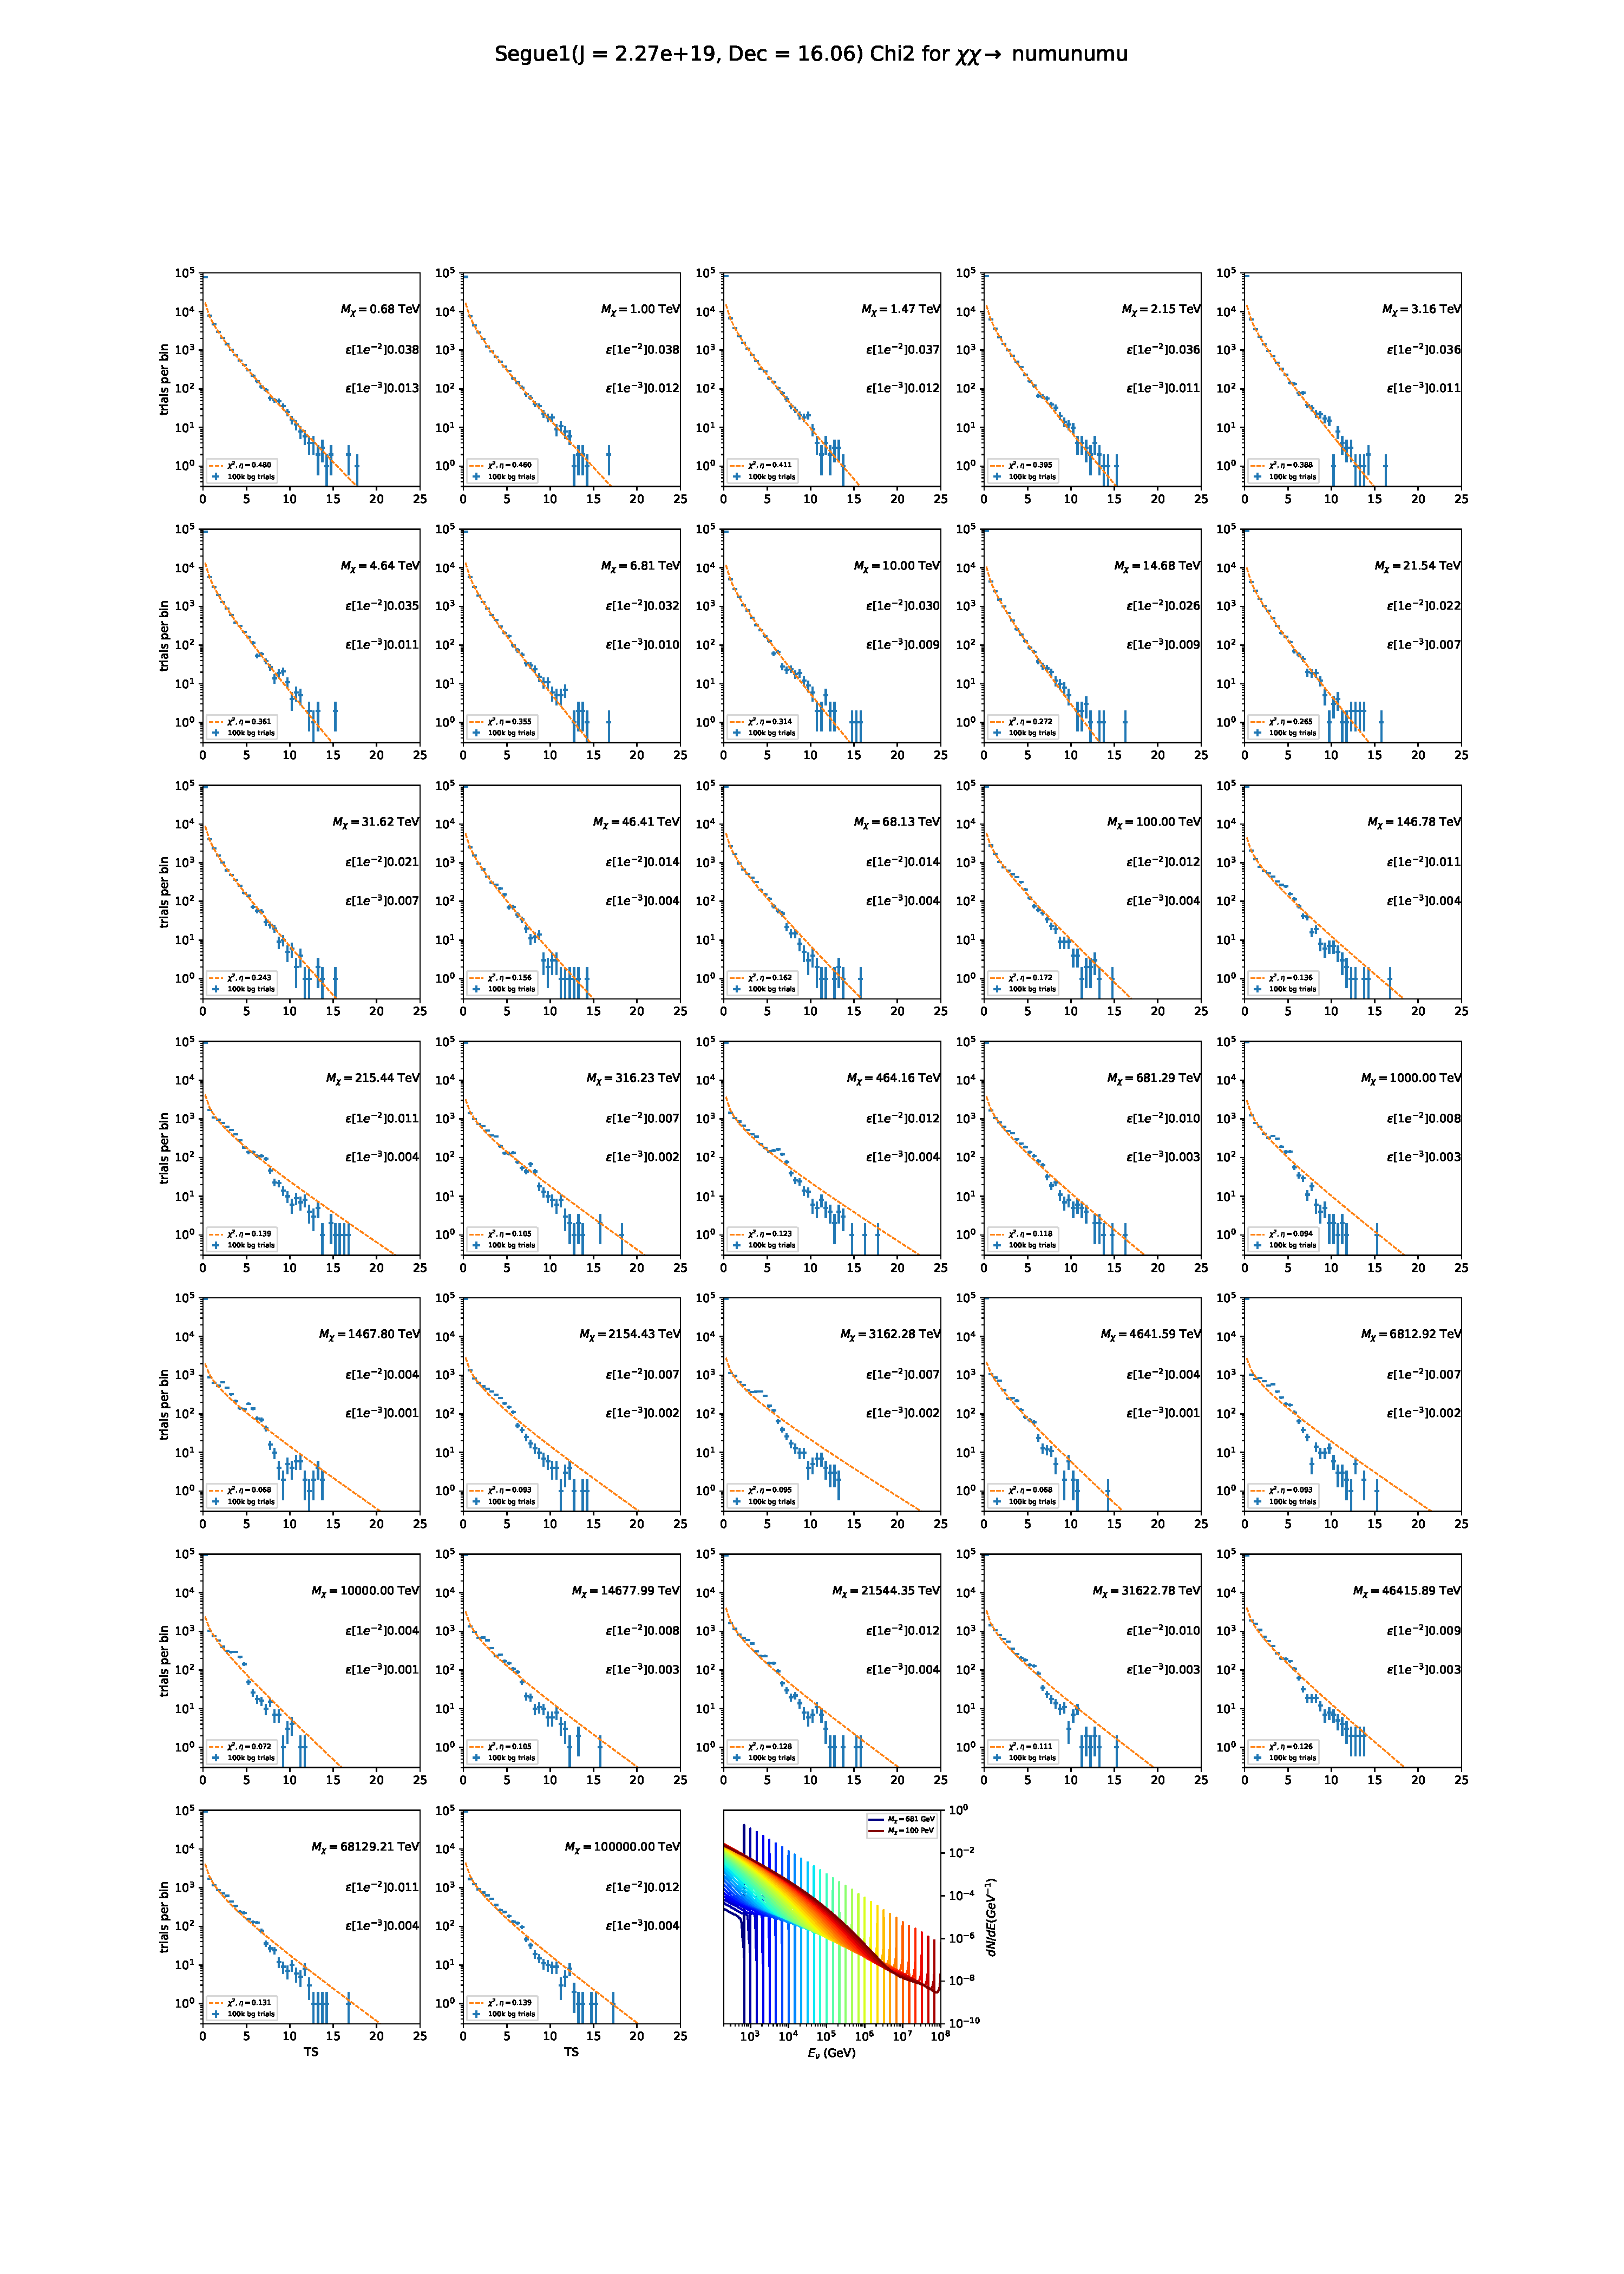
\includegraphics[clip, trim=22.1cm 6.5cm 19.5cm 56.5cm, scale=0.55]{figures/ic_DM/dm_plots/Segue1_numunumu_chi2_Masspanel_2024-03-23.pdf} &
            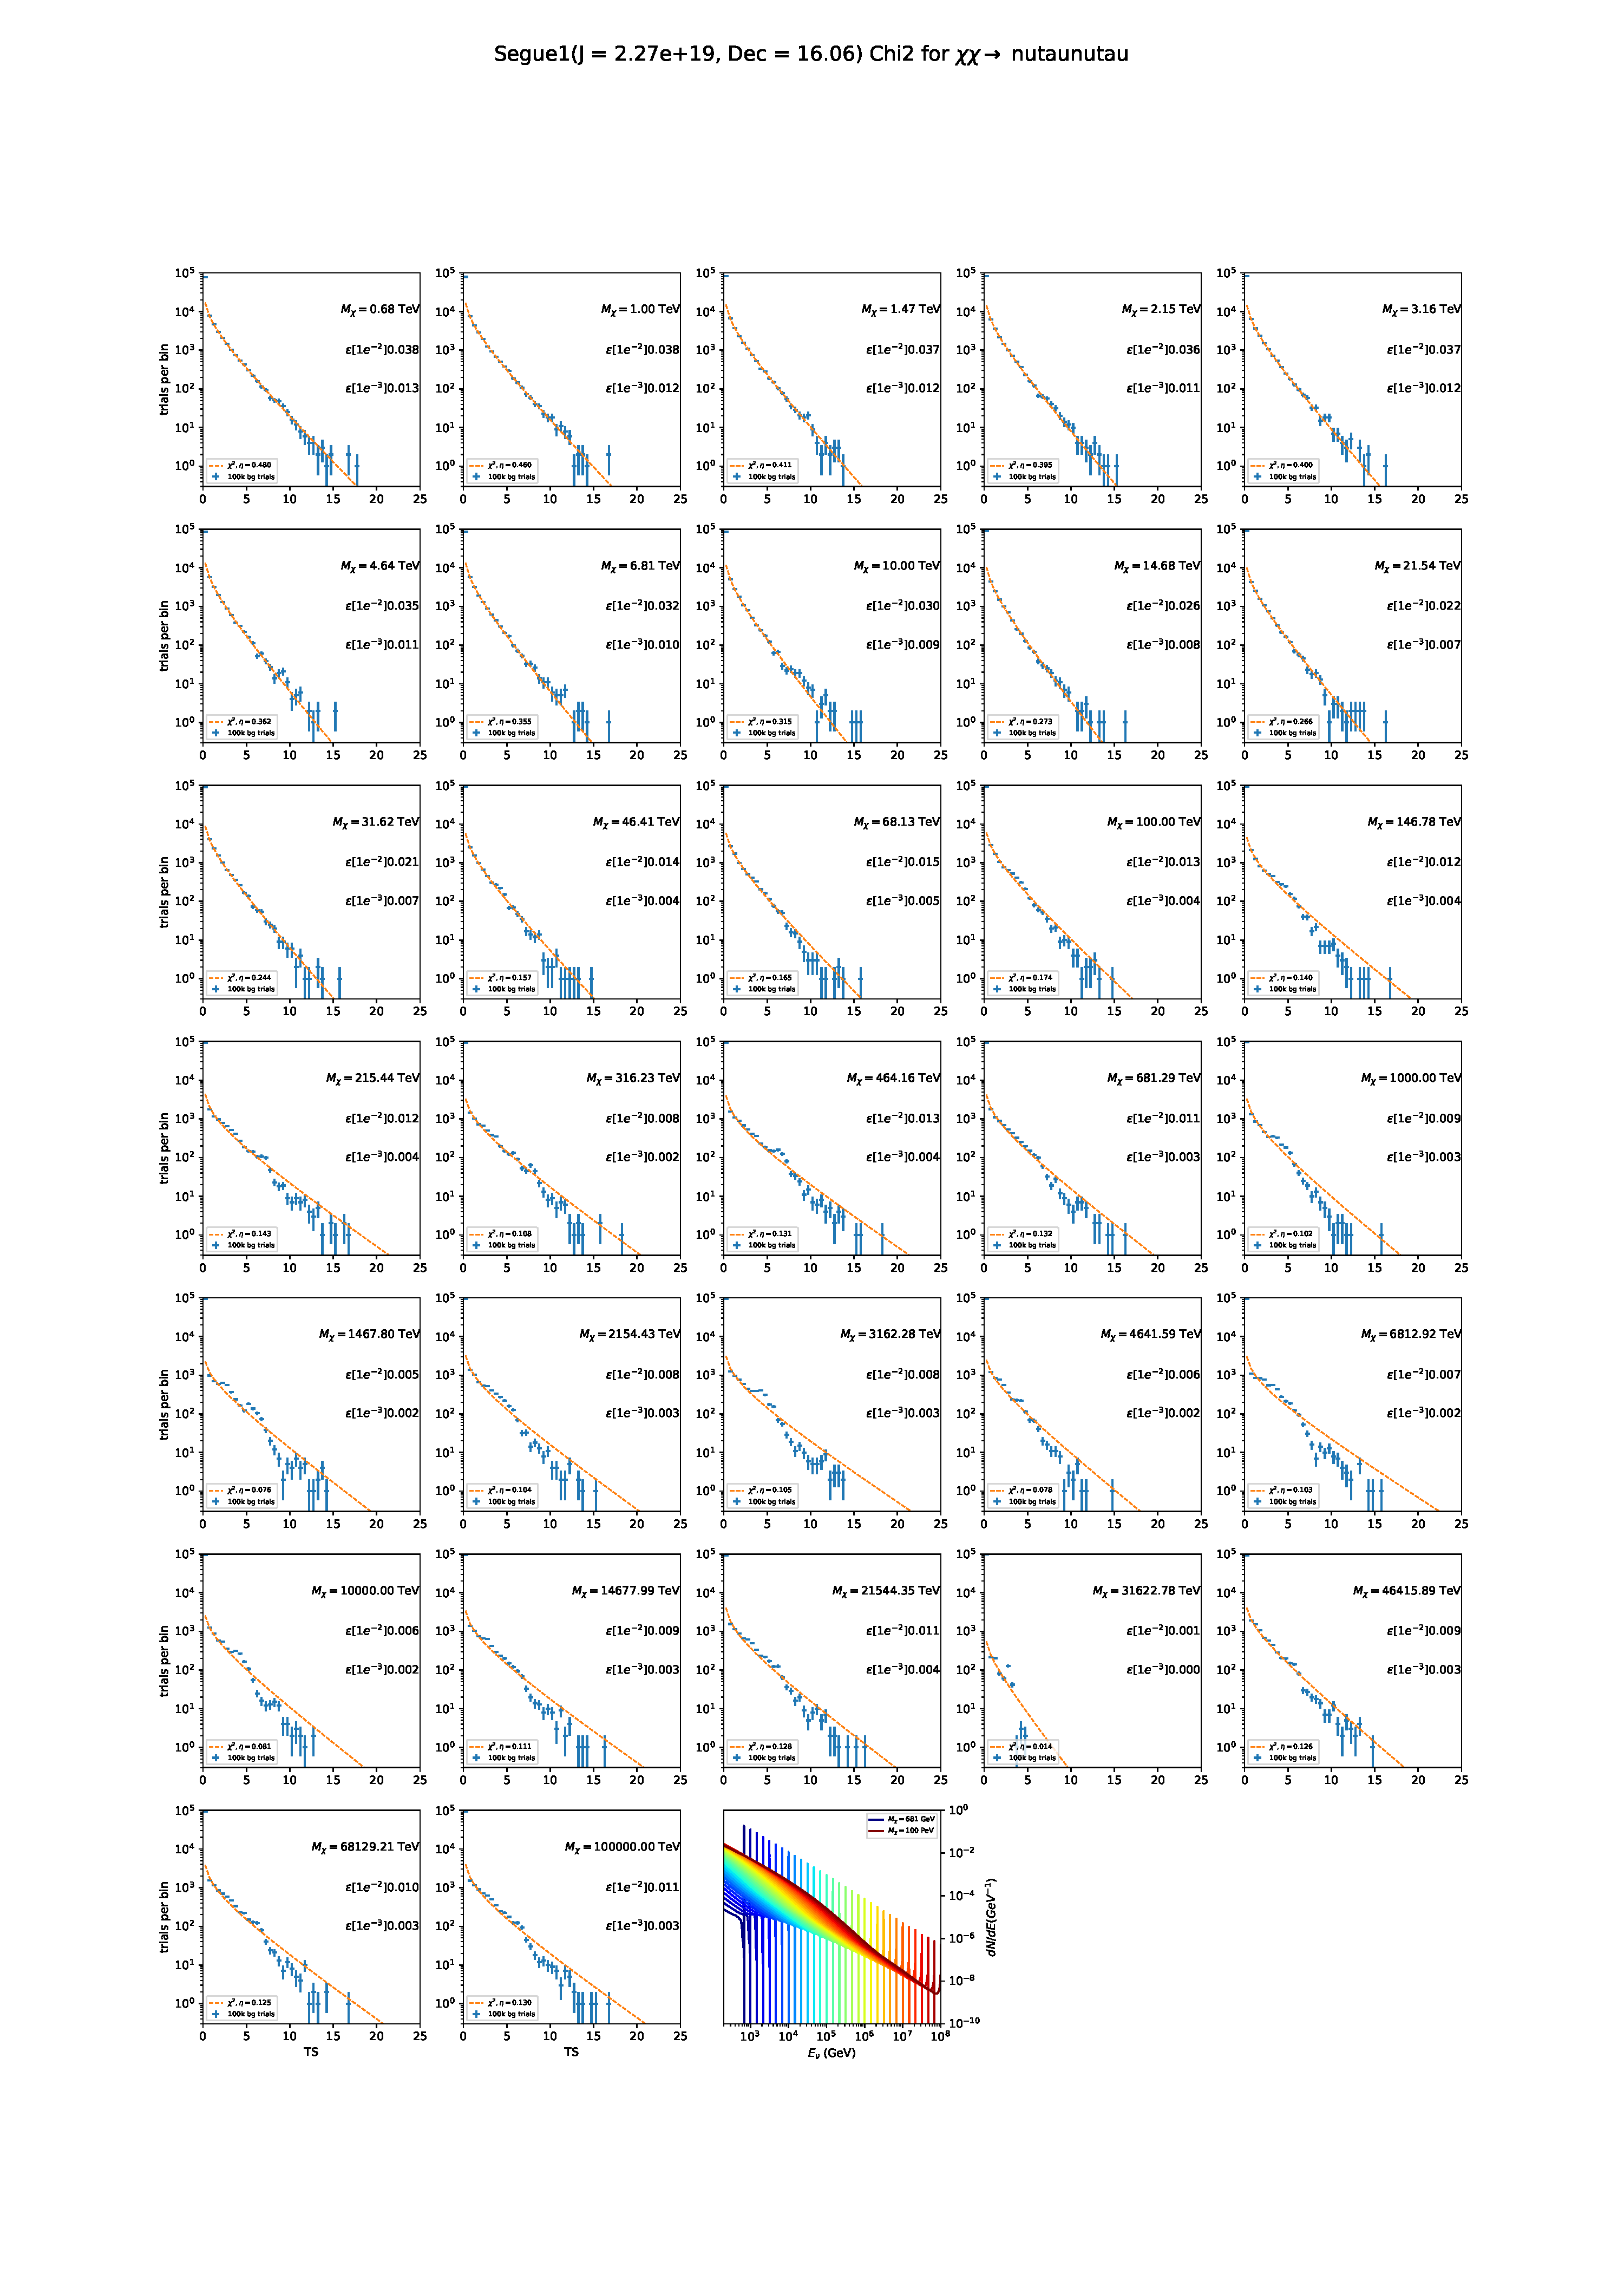
\includegraphics[clip, trim=22.1cm 6.5cm 19.5cm 56.5cm, scale=0.55]{figures/ic_DM/dm_plots/Segue1_nutaunutau_chi2_Masspanel_2024-03-23.pdf} \\
        \end{tabular}
    }\caption{Summary of input spectral models that were smoothed with Gaussian kernel. Spectral models are for $\chi\chi \rightarrow$ \parpar{e}, \parpar{\mu}\parpar{\tau}, \parpar{\nu_e}, \parpar{\nu_\mu}, and \parpar{\nu_\tau}. These spectra are the composite ($\nu_\mu$ + $\nu_\tau$) of neutrino flavors. Every spectral model used for this analysis is featured as a colored solid line. Bluer lines are for lower DM mass spectral models. DM masses range from 681 GeV to 100 PeV. HDM \cite{HDMSpectra}, $\chi$aro$\nu$ \cite{Charon}, and Photospline \cite{photospline} are used to generate these spectra. Energy (x-axis) was chosen to roughly represent the energy sensitivity of NST.}
    \label{fig:line_spectra_smooth}
\end{figure}

\Cref{fig:line_spectra_smooth} shows the spectral models that required Gaussian smoothing, the leptonic annihilation channels.
The remaining models where the only processing was spline fitting are documented in \cref{sec:apdx_final_specs}.
Notice that the different neutrino flavors are unique, especially in their low energy tails.
Therefore, this analysis will be sensitive to DM annihilating to the distinct neutrino flavors.

%%%%%%%%%%%%%%%%%%%%%%%%%%%%%%%%%%%%%%%%%%%%%%%%%%
\subsection{\J - Astrophysical Component}\label{sec:icDM_spatialmodel}
%%%%%%%%%%%%%%%%%%%%%%%%%%%%%%%%%%%%%%%%%%%%%%%%%%

For this analysis, we re-adopt the \GS model used in \cref{sec:glory_duck} for dSph from \cite{Geringer_Sameth_2015}.
These models are based on a modified Navarro-Frenk-While (NFW) profile where the indices of the NFW (traditionally 1,3,1) are allowed to float.
The angular width of these sources is much smaller than the angular resolution of IceCube NST \cite{IC_NGC1068}.
We therefore treat these sources as point sources in this analysis, and forgo generating maps.
Theses sources and the \GS model have already been discussed at length in \cref{sec:gd_spatialmodel} and is not repeated here.
IceCube uses identical sources to \cref{tab:gd_J_factor} except we analyze source with declinations above 0.0 degrees.

%%%%%%%%%%%%%%%%%%%%%%%%%%%%%%%%%%%%%%%%%%%%%%%%%%
\subsection{Source Selection and Annihilation Channels}\label{sec:ic3_study_selection}
%%%%%%%%%%%%%%%%%%%%%%%%%%%%%%%%%%%%%%%%%%%%%%%%%%

We use all of the dSphs presented in IceCube's previous dSph DM search \cite{IC3_DM2013}.
IceCube's sources for these simulation studies include Bootes I, Canes Venatici I, Canes Venatici II, Coma Berenices, Draco, Hercules, Leo I, Leo II, Leo V, Leo T, Segue 1, Segue 2, Ursa Major I, Ursa Major II,  and Ursa Minor.
A full description of all sources used is in \Cref{tab:gd_J_factor}.
Sources with declinations less than 0.0 are excluded from this analysis.

This analysis improves on the previous IceCube dSph paper \cite{IC3_DM2013} in the following ways.
Previously, the IceCube detector was not yet completed to the 86 string configuration.
Many more dSphs will be observed, from 4 to 15.
Previously, the particle physics model used for neutrino-ray spectra from DM annihilation did not have EW corrections where they are now included \cite{HDMSpectra}.
The spectral models also predict substantial differences between the neutrino flavors, so this analysis will be the first DM dwarf analysis to discriminate between primary neutrino flavors.
The study performed here studies 10.4 years of data.

The SM annihilation channels probed for this study include $\chi\chi \rightarrow$
\begin{itemize}
    \item[] \parpar{b}, \parpar{t}, \parpar{u}, \parpar{d}, \parpar{e}, \parpar{\mu}, \parpar{\tau}, \pp{Z}, $W^+W^-$, \parpar{\nu_e}, \parpar{\nu_\mu}, and \parpar{\nu_\tau}
\end{itemize}

%%%%%%%%%%%%%%%%%%%%%%%%%%%%%%%%%%%%%%%%%%%%%%%%%%
\section{Likelihood Methods}\label{sec:icDM_LLH}
%%%%%%%%%%%%%%%%%%%%%%%%%%%%%%%%%%%%%%%%%%%%%%%%%%

I use the Point-Source search likelihood which is widely used in IceCube analyses.
The likelihood function is defined as the following:
\icPtSrcLLH
where  $ i $ is an event index, $S$ and $B$ are the signal PDF and background PDF respectively. For a joint analysis where the sources are stacked the likelihood is expanded in the simplified way:
\icStackLLH
Where $ L_i $ is the likelihood from the i-th source in the stacked analysis.
The Test Statistic (TS) definition remains the same as \cref{eq:gd_TS}

%%%%%%%%%%%%%%%%%%%%%%%%%%%%%%%%%%%%%%%%%%%%%%%%%%
\section{Background Simulation}\label{sec:icDM_bkgd_sim}
%%%%%%%%%%%%%%%%%%%%%%%%%%%%%%%%%%%%%%%%%%%%%%%%%%

Before we look at data, we must first analyze background and signal injection to validate our anlysis.
This is in part because the TS distributions are not expected to behave according to a chi-squared distribution with 1 degree of freedom.
TS distributions can also vary significantly between DM mass and annihilation models.
Therefor, Wilks' theorem may not be applicable to the analysis.
Instead, a critical value is defined from a large number of background trials.
We study the TS distributions first for each source, then for the stacked analysis.
The following sections show the results of the likelihood fitting for a suite of background trials.

I assume that TS values are physical: $ \mathrm{TS} \ge 0 $.
$\eta$ denotes the fraction of positive TS values above the threshold and written in the legend of the TS distributions.
$ \epsilon[x] $ indicate the fraction of events where $ \mathrm{TS} < x $. For TS plots shown here, the decimal values of x are 1.0e-2 and 1.0e-3.
Each subplot represents a simulation of 100,000 data-scrambled background trials.
\Cref{sec:icD_sec:icDM_TSperSrc} show the background TS distributions obtained from Segue 1, a source with little Earth attenuation and large \J-factor, and Ursa Major II, similarly large \J-fator but significantly more Earth attenuation, assuming that dark matter annihilates into \parpar{b}, \parpar{\tau}, and \parpar{\nu_\mu}.
I show the TS distributions of a stacked study of 15 sources for all DM annihilation channels.

%%%%%%%%%%%%%%%%%%%%%%%%%%%%%%%%%%%%%%%%%%%%%%%%%%
\subsection{TS per Source} \label{sec:icDM_TSperSrc}
%%%%%%%%%%%%%%%%%%%%%%%%%%%%%%%%%%%%%%%%%%%%%%%%%%

\Cref{fig:icDM_Seg1bb_TS} to \Cref{fig:icDM_UMa2numu_TS} present the TS distributions for Segue 1 and Ursa Major II for 100,000 trials.
More studies for all annihilation channels and remaining 13 sources were also performed and are documented in IceCube's internal wiki.

Although it was not expected, almost every distribution produced follows a $\chi^2$ distribution with 1 degree of freedom.
This is important for future assumptions made in \cref{sec:nu_duck} and may justify statistical calculations assuming Wilk's theorem is valid.

\begin{figure}[ht]
    \centering{
        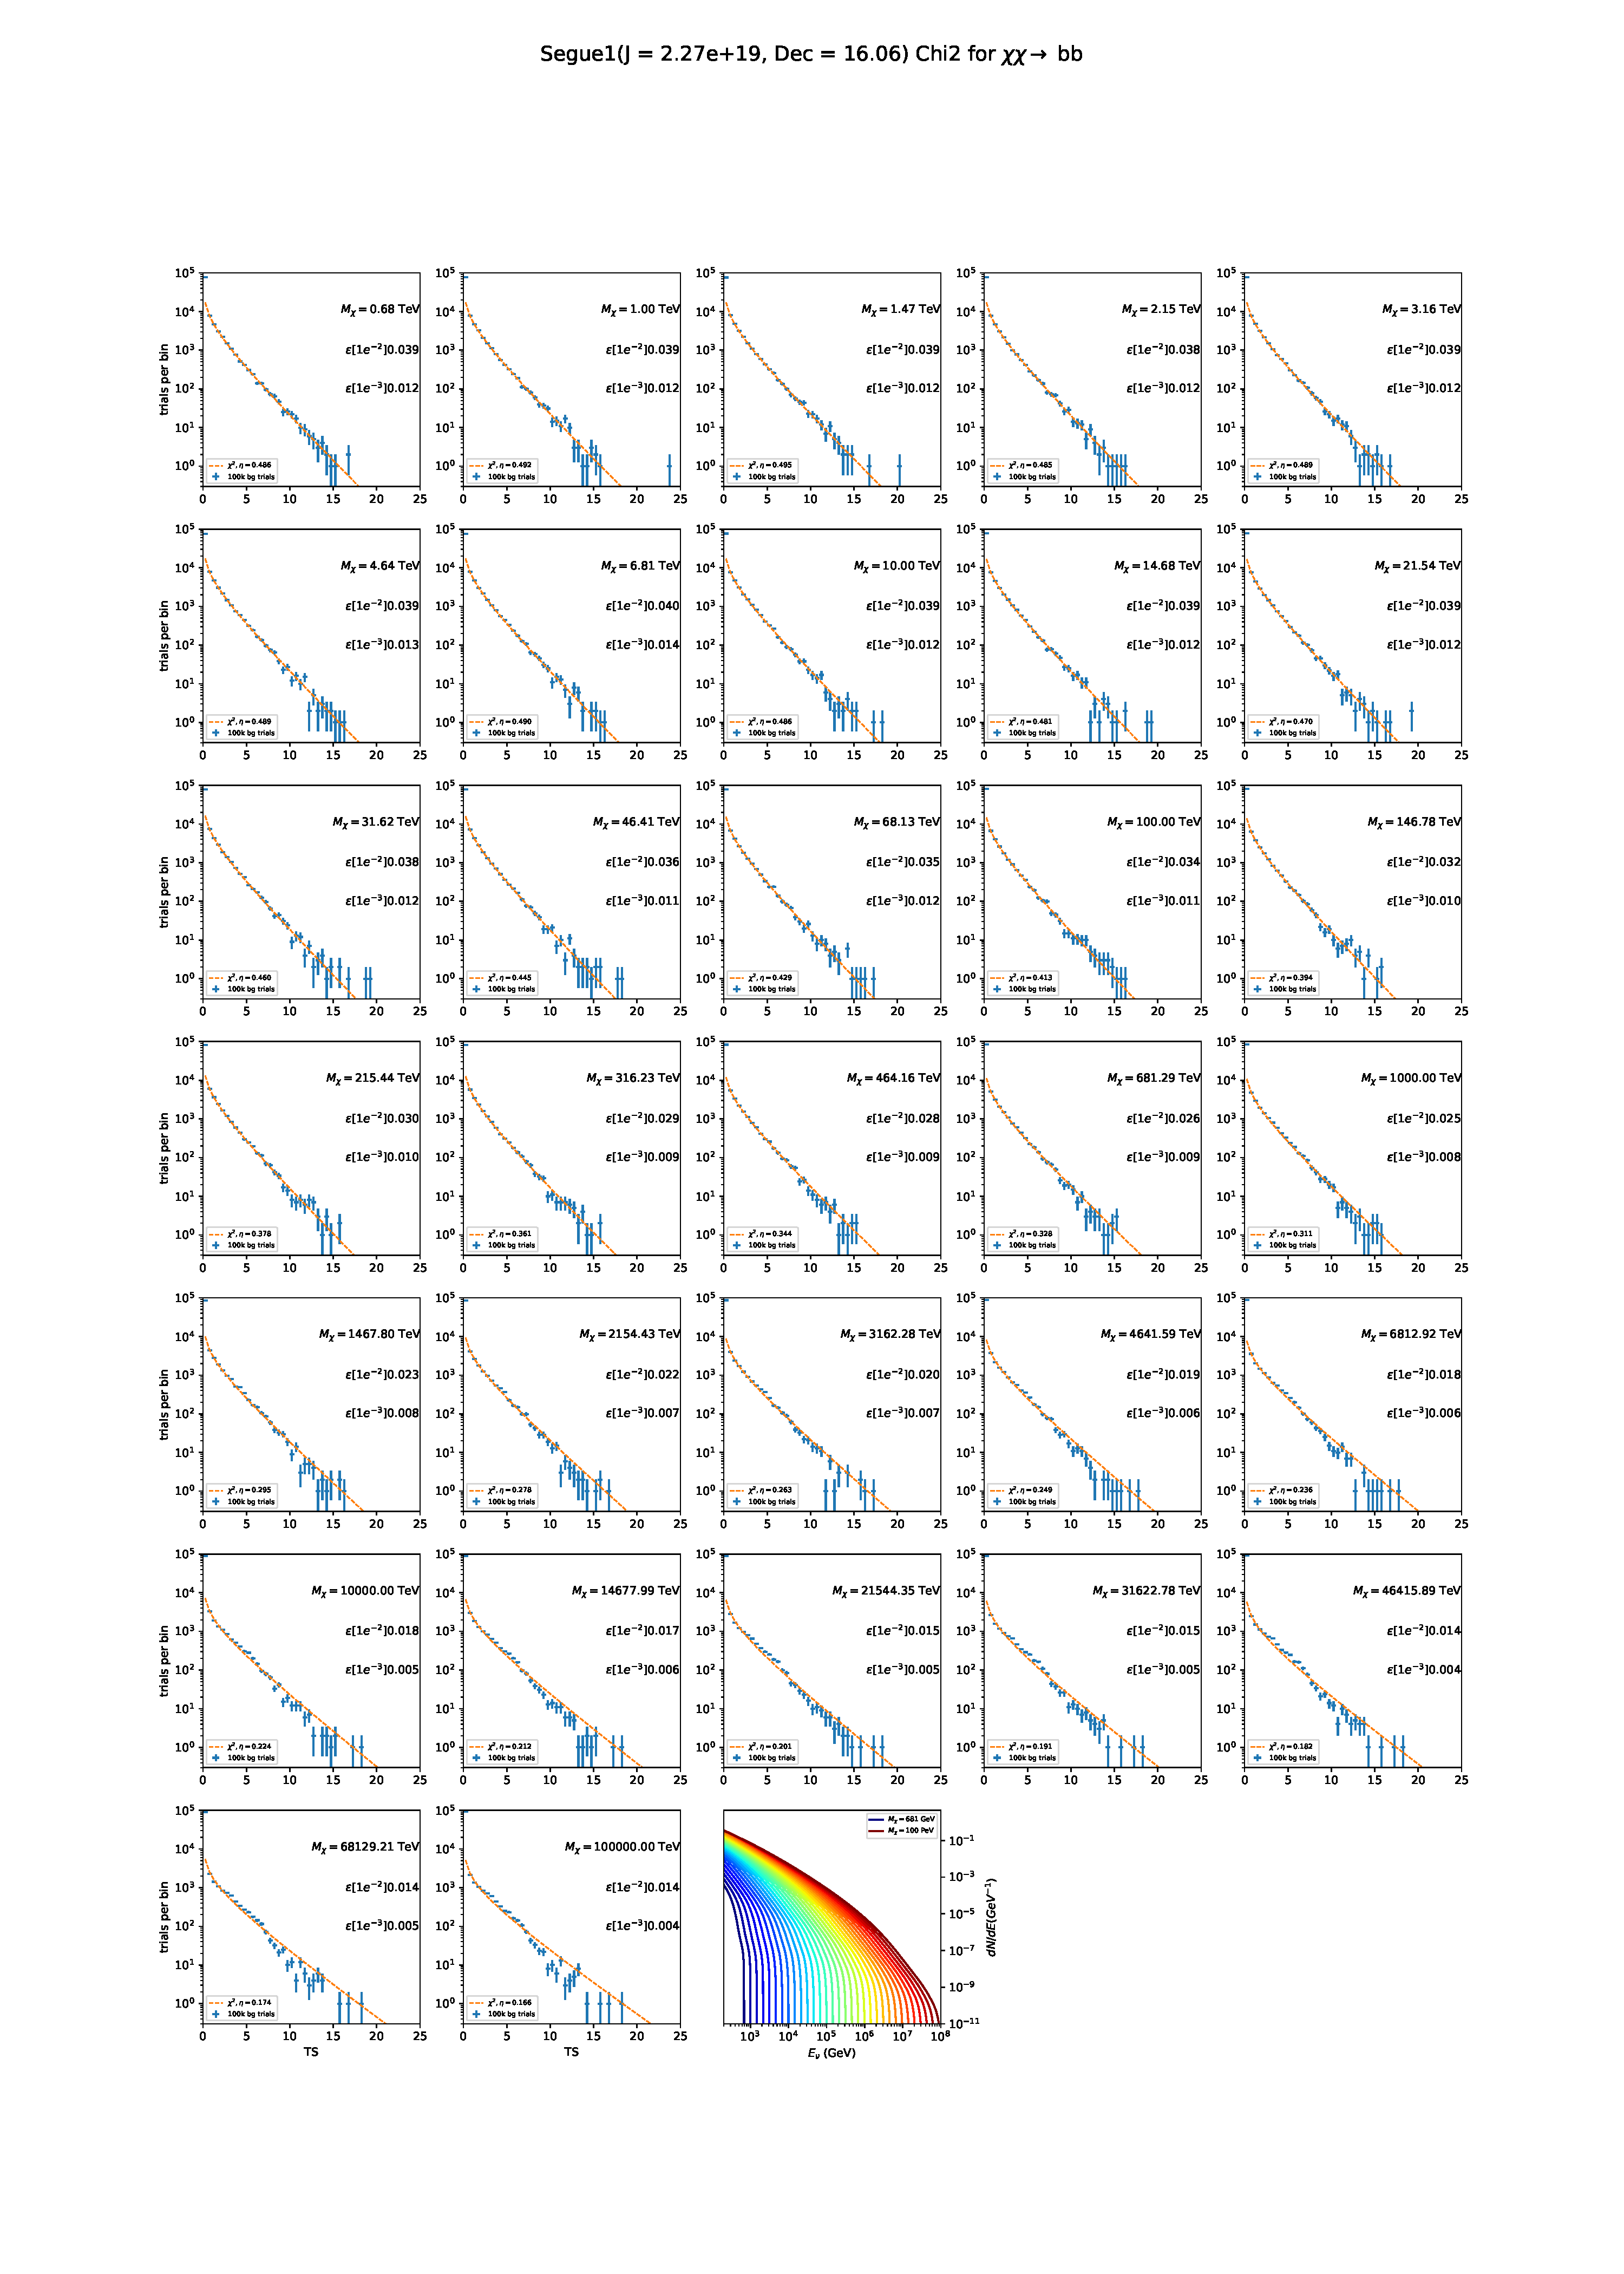
\includegraphics[clip, trim=5cm 6.5cm 4.9cm 8cm, scale=0.345]{figures/ic_DM/dm_plots/Segue1_bb_chi2_Masspanel_2024-03-23.pdf}
    }\caption{Test statistic (TS) distributions for Segue 1 and $\chi\chi \rightarrow$ \parpar{b}. Each subplot, except the final, is the TS distribution for a specific DM mass listed in the subplot. Orange dashed lines are the traces for a $\chi^2$ distribution with 1 degree of freedom. $\epsilon[\cdot]$ is the fraction of trials smaller than the bracketed value. The final subplot plots the all DM spectral models, similar to \cref{fig:line_spectra_smooth}, used as input for the TS distributions.}
    \label{fig:icDM_Seg1bb_TS}
\end{figure}

\begin{figure}[ht]
    \centering{
        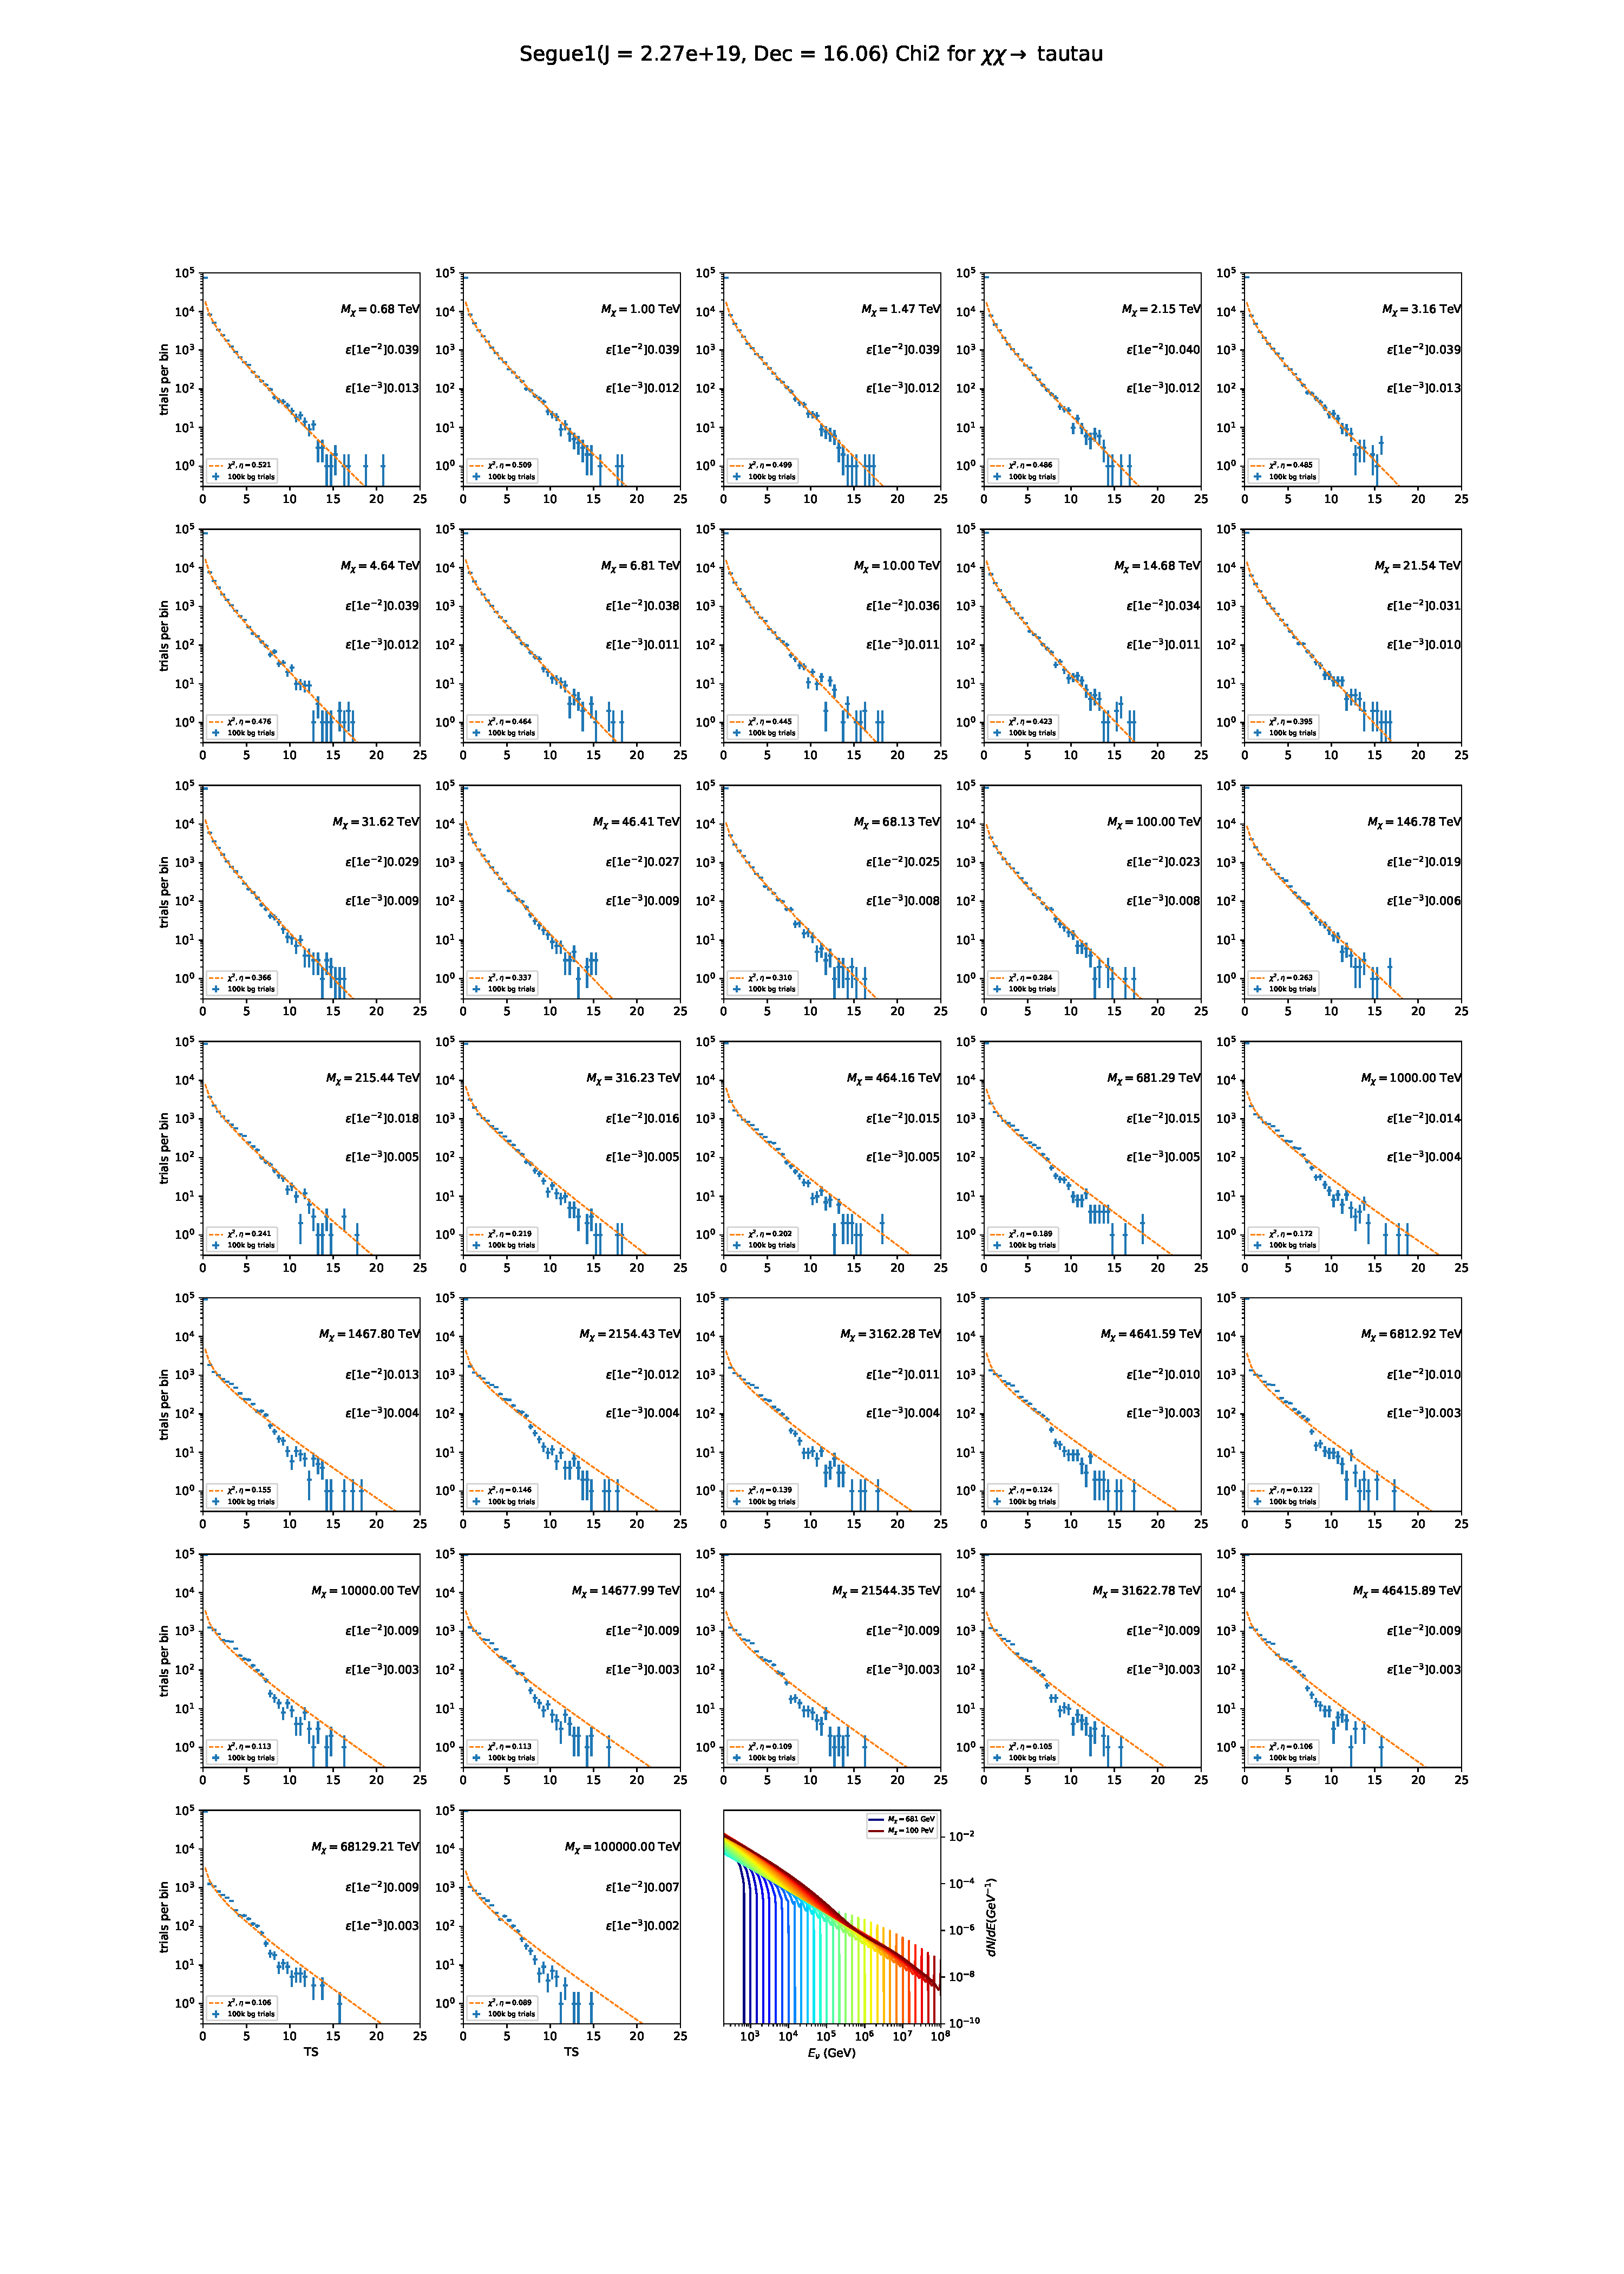
\includegraphics[clip, trim=5cm 6.5cm 4.9cm 8cm, scale=0.345]{figures/ic_DM/dm_plots/Segue1_tautau_chi2_Masspanel_2024-03-23.pdf}
    }\caption{Same as \cref{fig:icDM_Seg1bb_TS} for Segue 1 $\chi\chi \rightarrow$ \parpar{\tau}.}
    \label{fig:icDM_Seg1tau_TS}
\end{figure}

\begin{figure}[ht]
    \centering{
        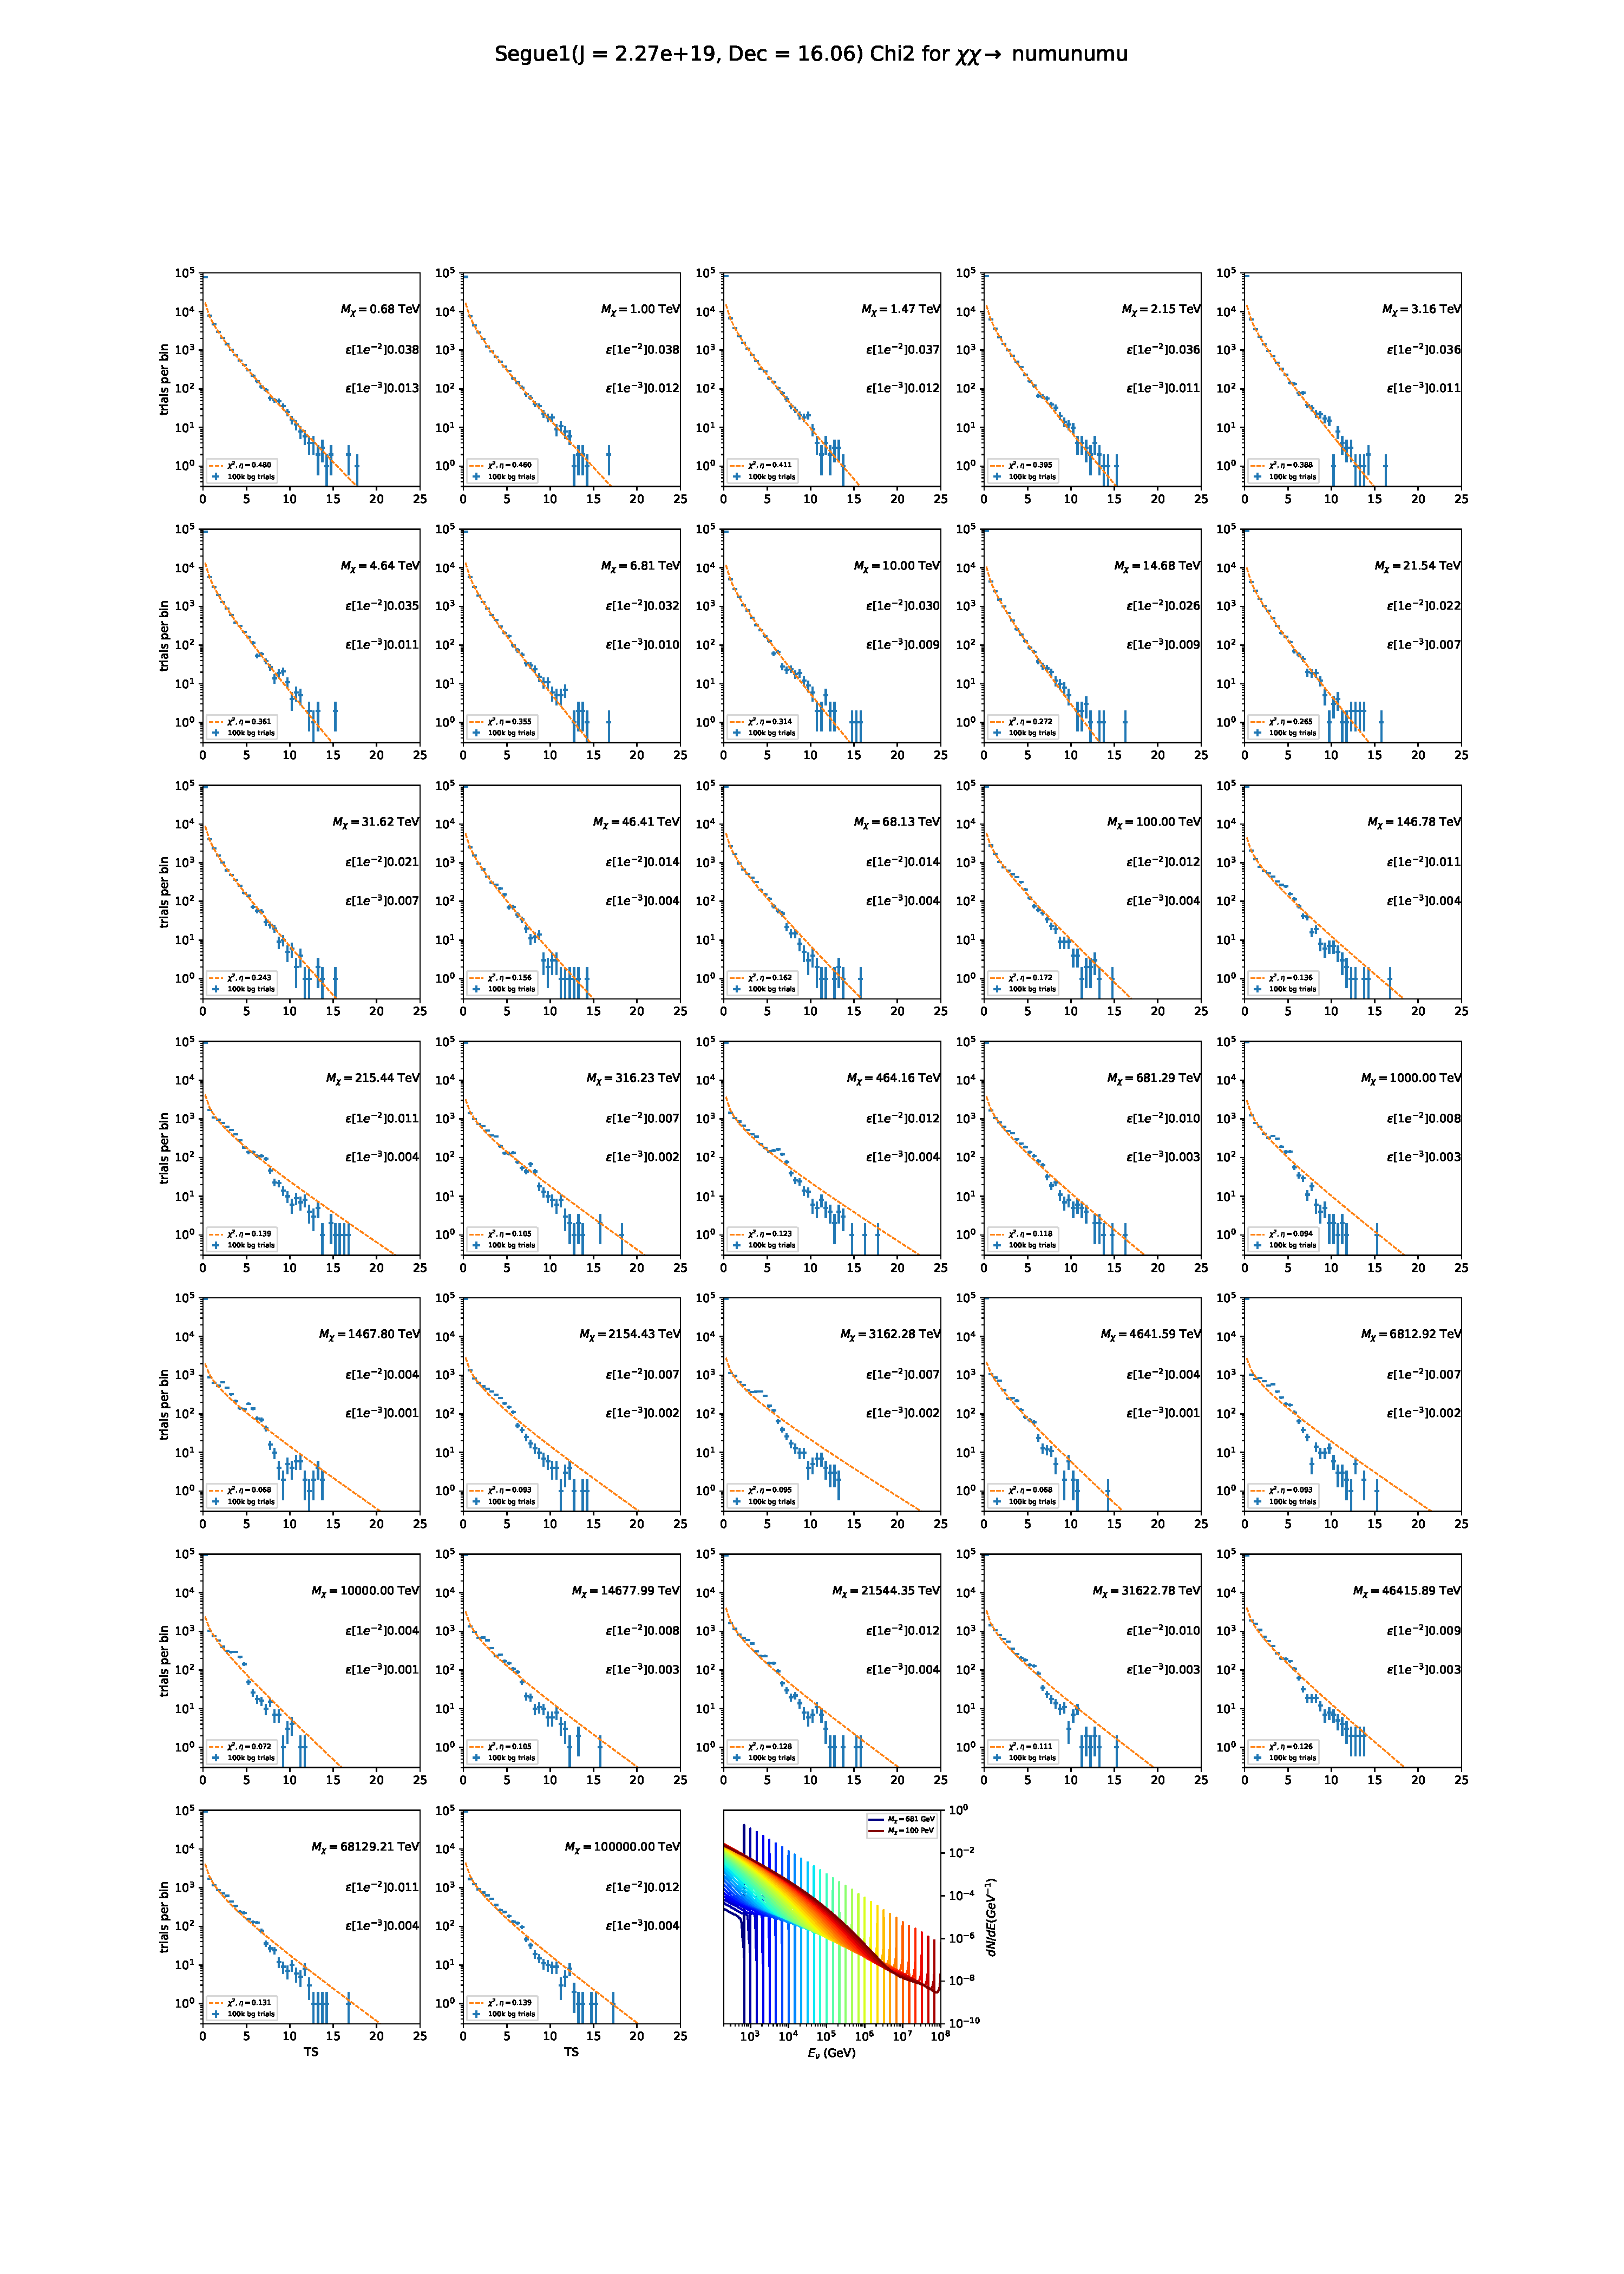
\includegraphics[clip, trim=5cm 6.5cm 4.9cm 8cm, scale=0.345]{figures/ic_DM/dm_plots/Segue1_numunumu_chi2_Masspanel_2024-03-23.pdf}
    }\caption{Same as \cref{fig:icDM_Seg1bb_TS} for Segue 1 $\chi\chi \rightarrow$ \parpar{\nu_\mu}.}
    \label{fig:icDM_Seg1numu_TS}
\end{figure}

\begin{figure}[ht]
    \centering{
        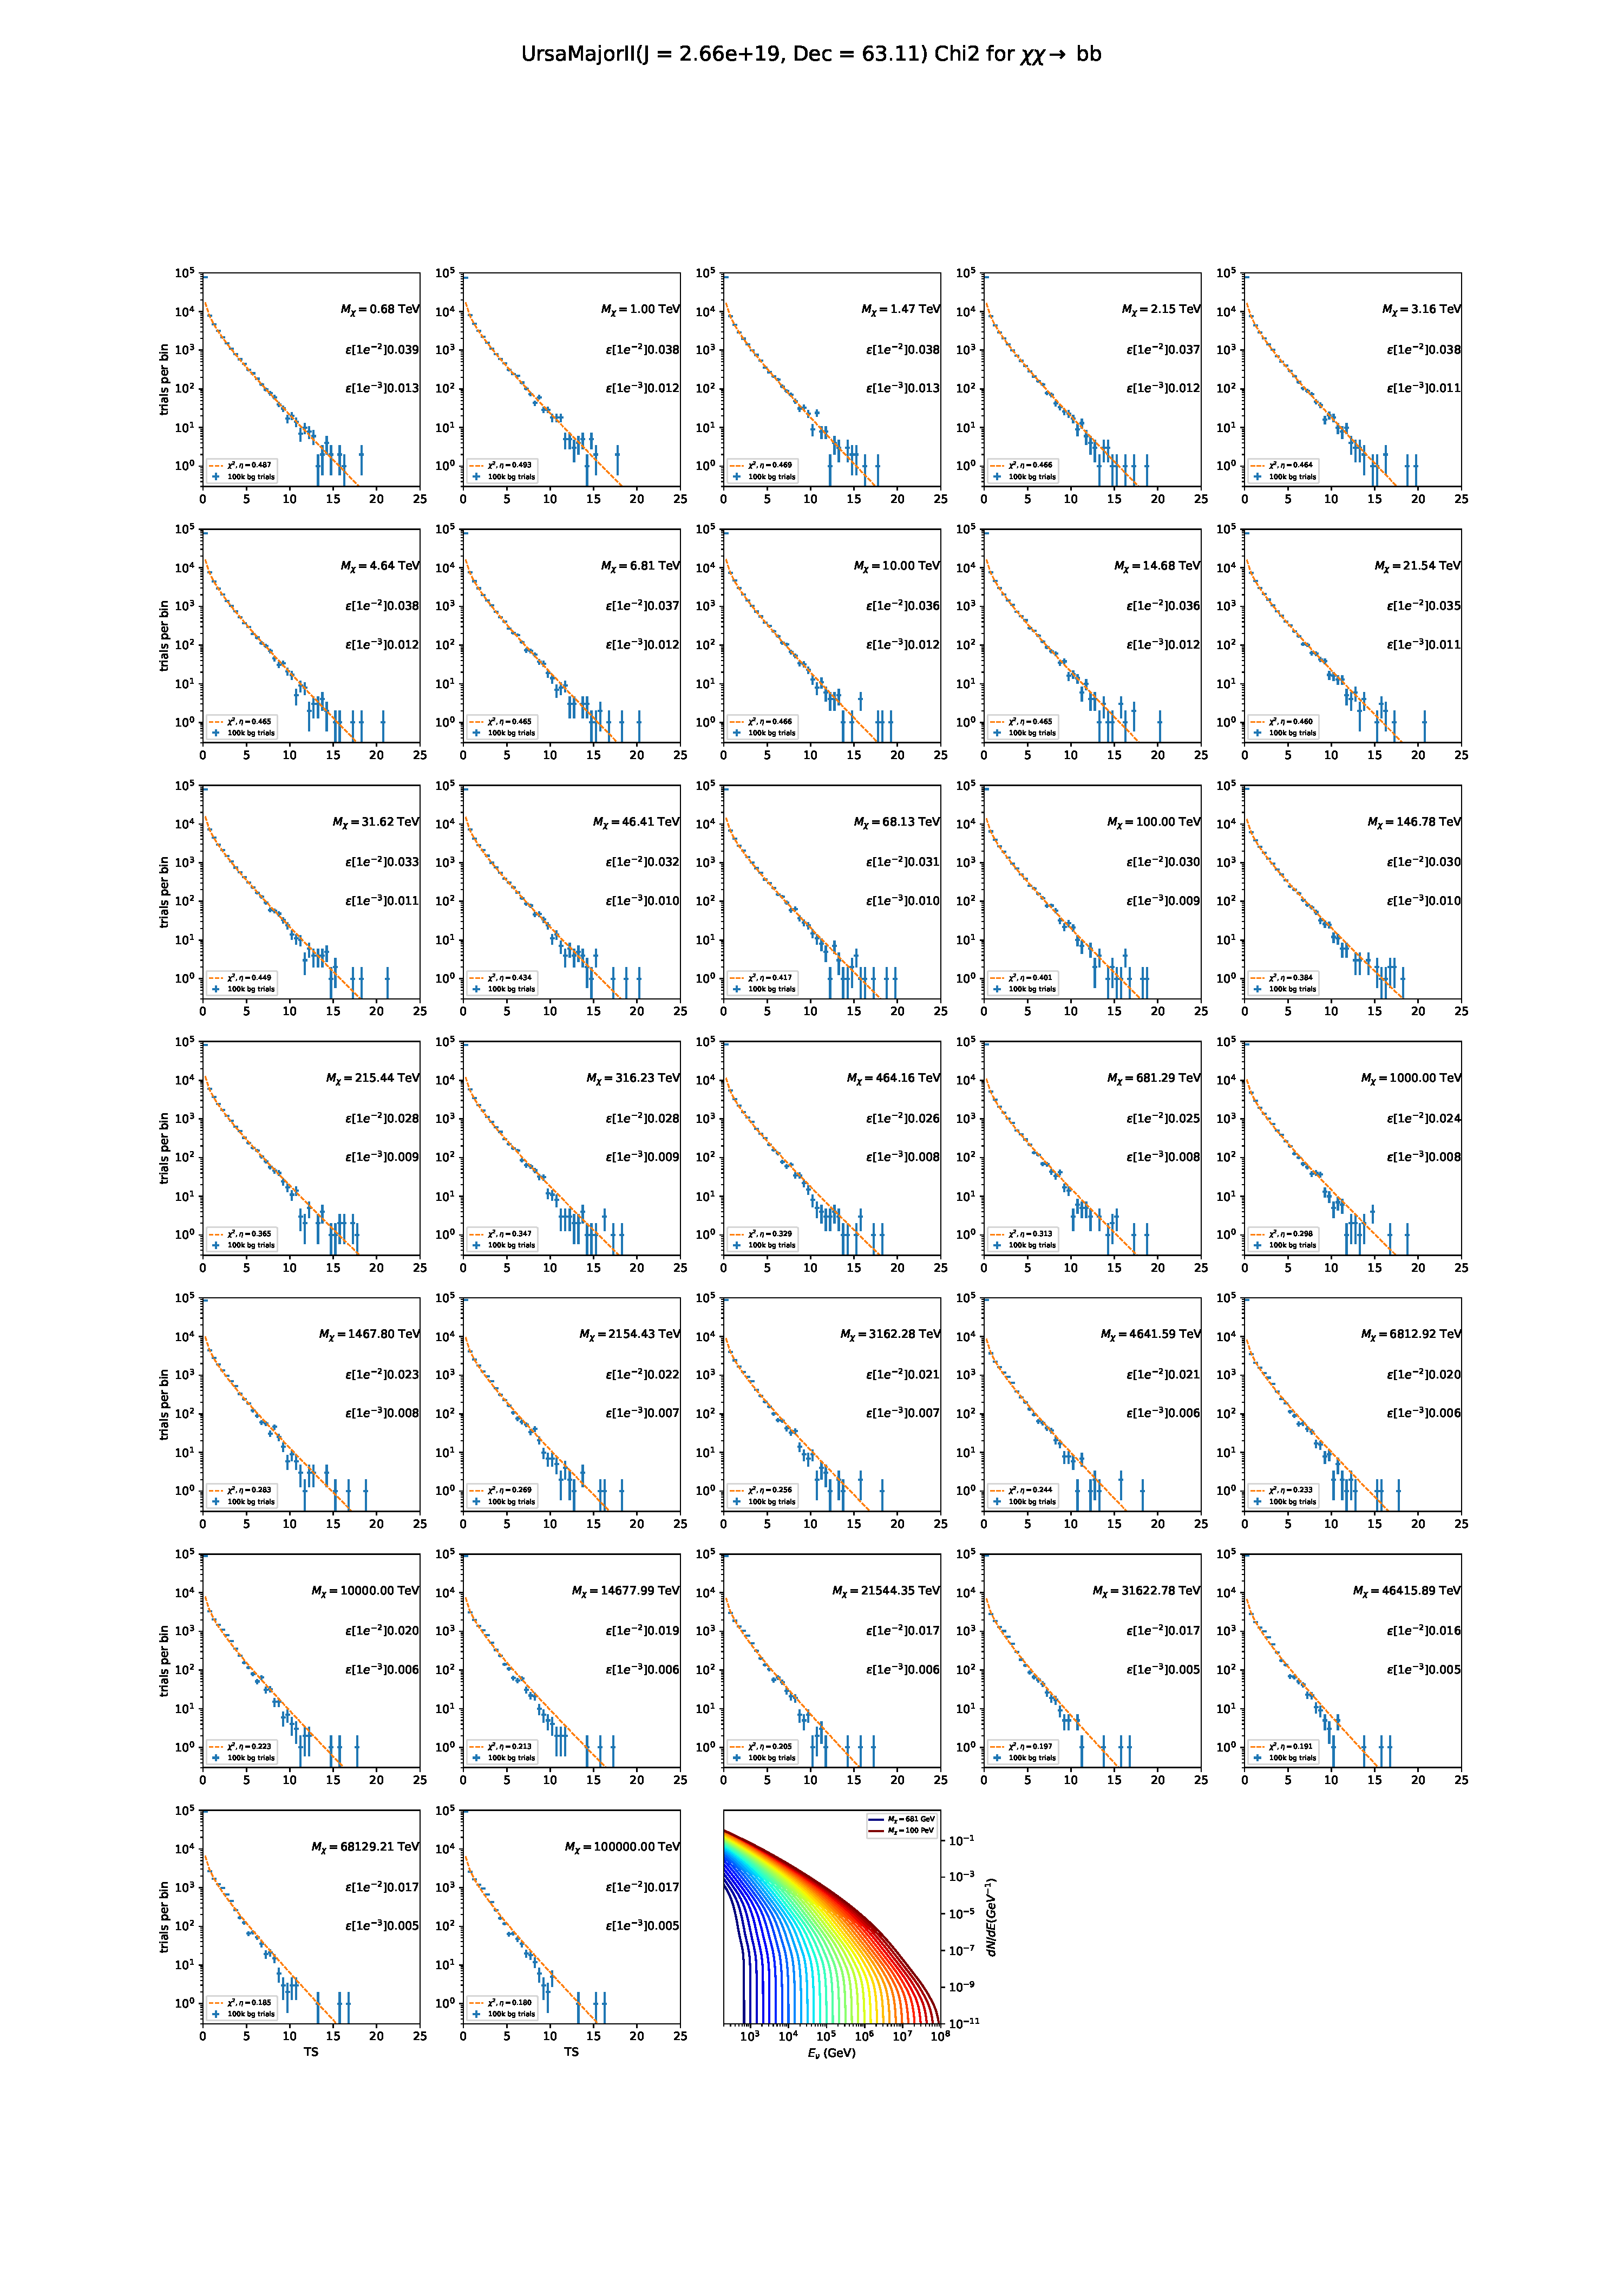
\includegraphics[clip, trim=5cm 6.5cm 4.9cm 8cm, scale=0.345]{figures/ic_DM/dm_plots/UrsaMajorII_bb_chi2_Masspanel_2024-03-23.pdf}
    }\caption{Same as \cref{fig:icDM_Seg1bb_TS} for Ursa Major II 1 $\chi\chi \rightarrow$ \parpar{b}.}
    \label{fig:icDM_UMa2bb_TS}
\end{figure}

\begin{figure}[ht]
    \centering{
        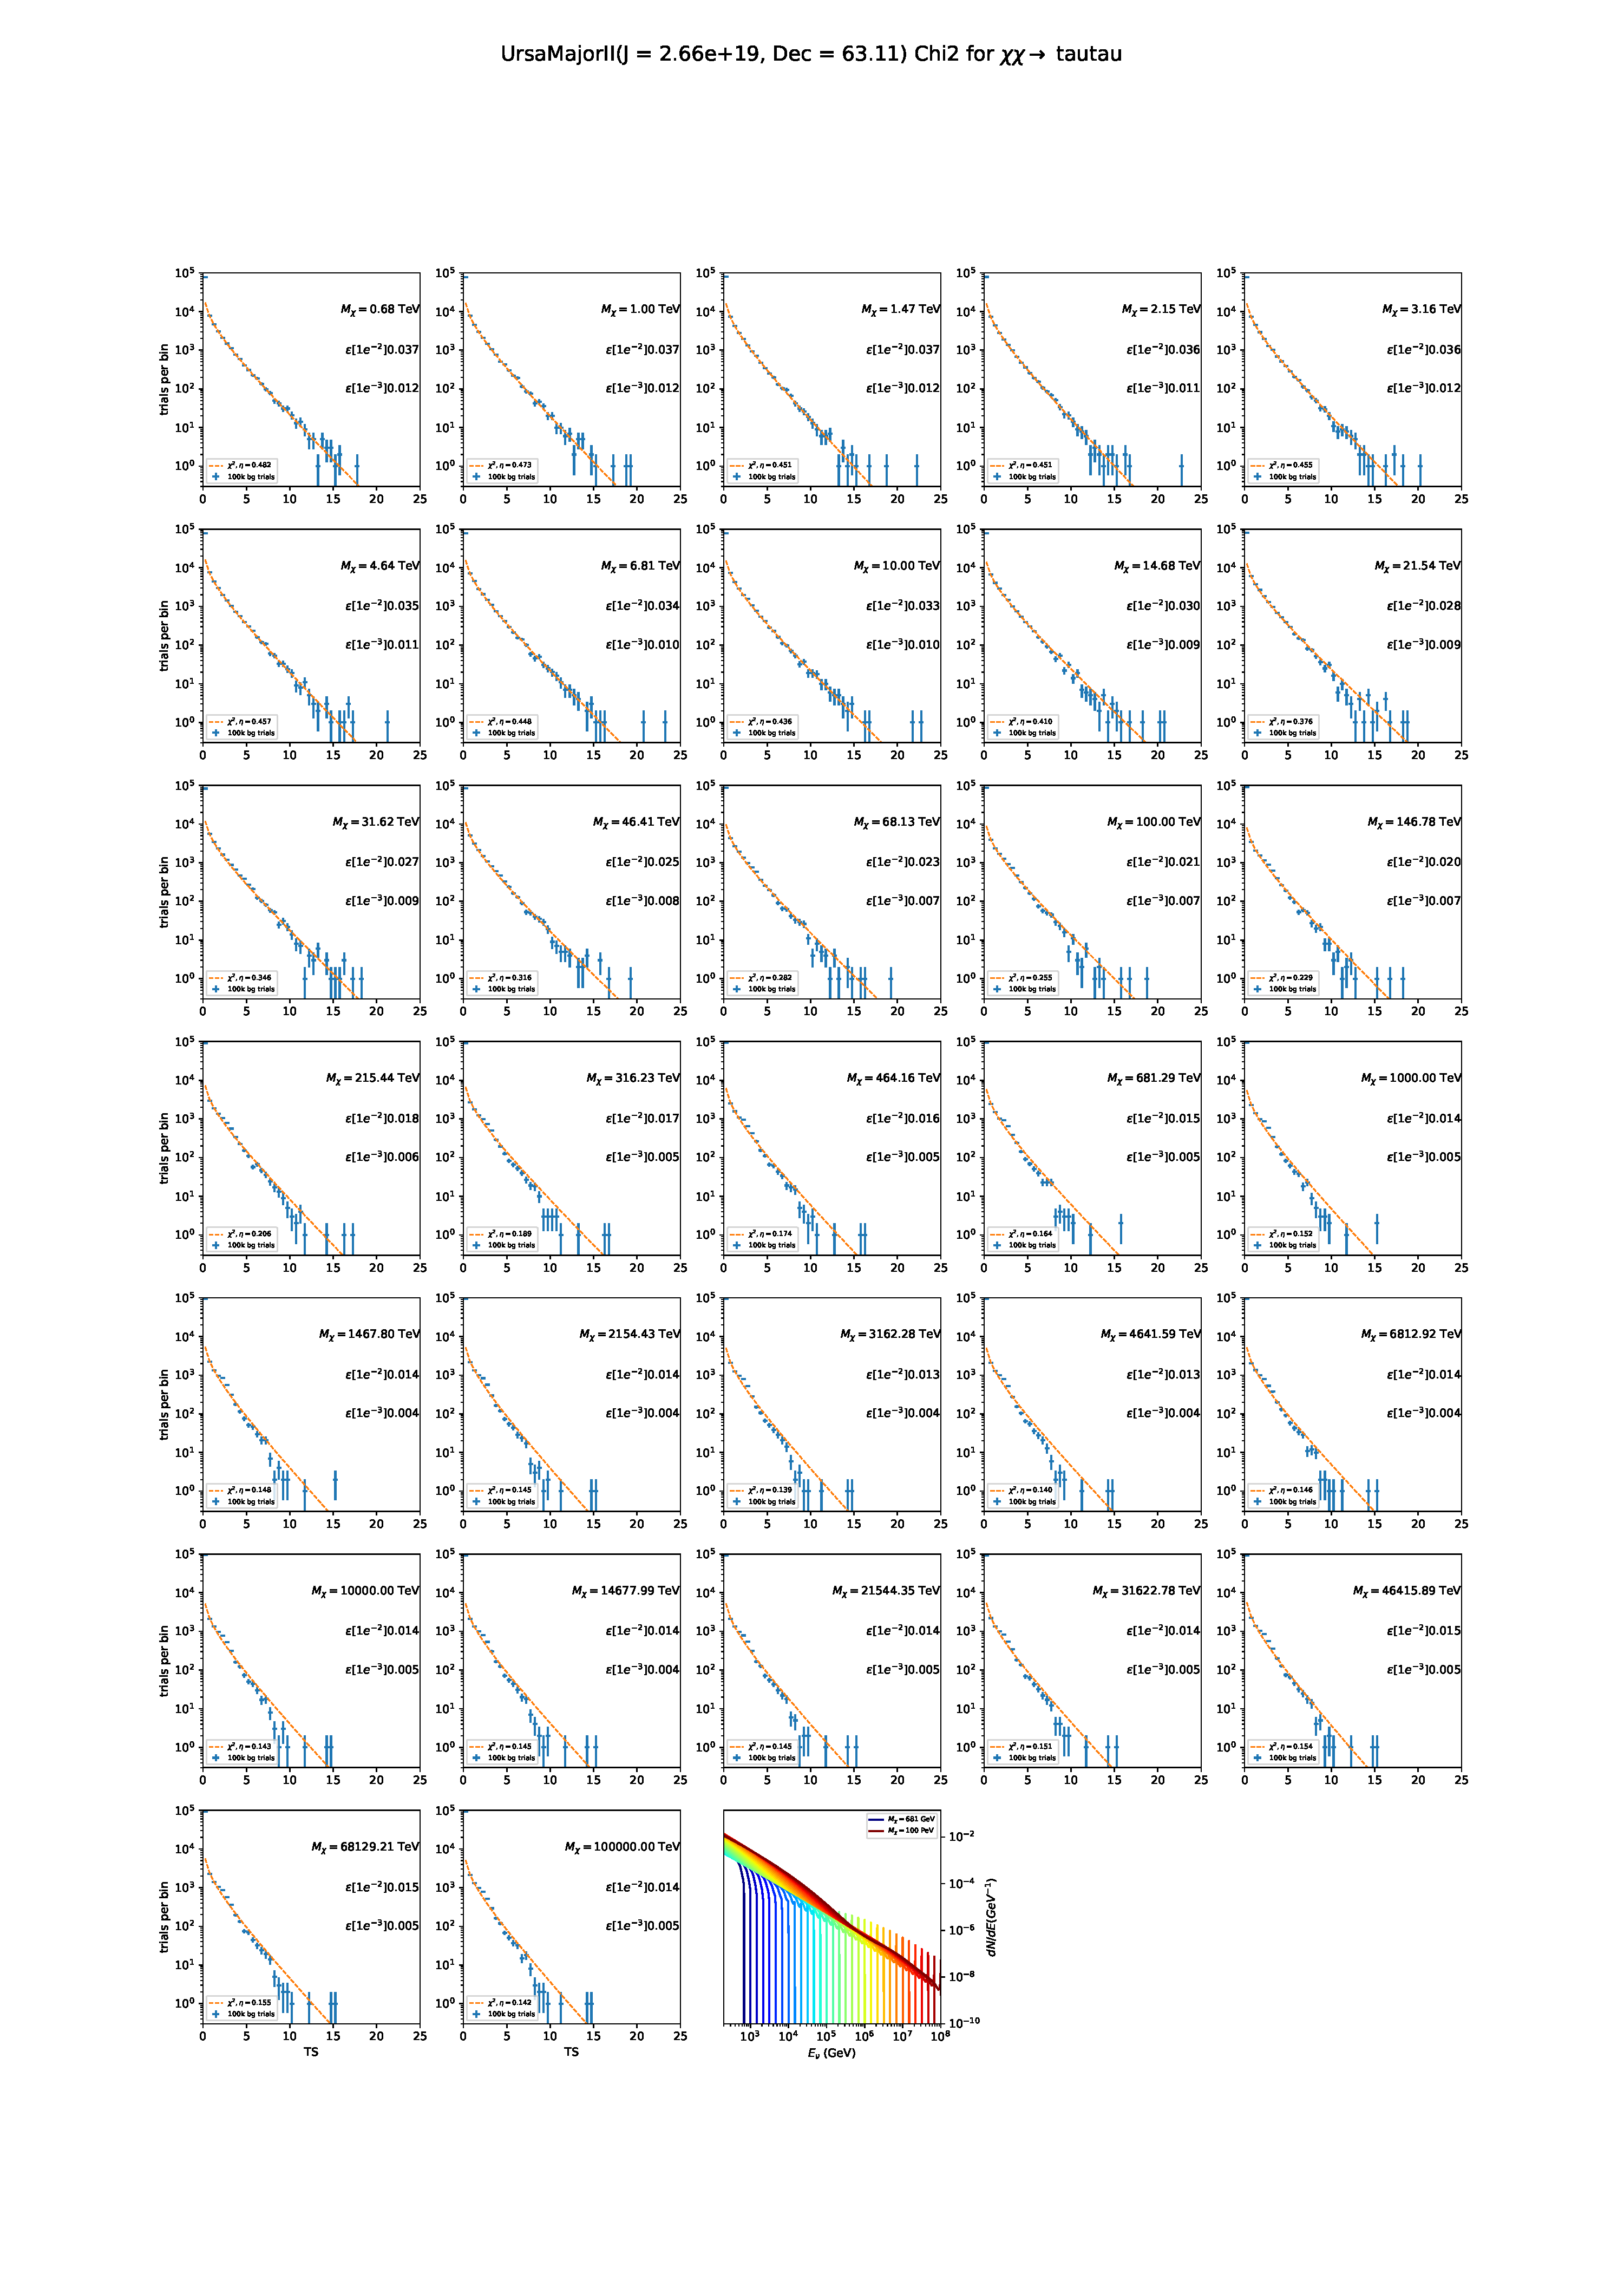
\includegraphics[clip, trim=5cm 6.5cm 4.9cm 8cm, scale=0.345]{figures/ic_DM/dm_plots/UrsaMajorII_tautau_chi2_Masspanel_2024-03-23.pdf}
    }\caption{Same as \cref{fig:icDM_Seg1bb_TS} for Ursa Major II 1 $\chi\chi \rightarrow$ \parpar{\tau}.}
    \label{fig:icDM_UMa2tau_TS}
\end{figure}

\begin{figure}[ht]
    \centering{
        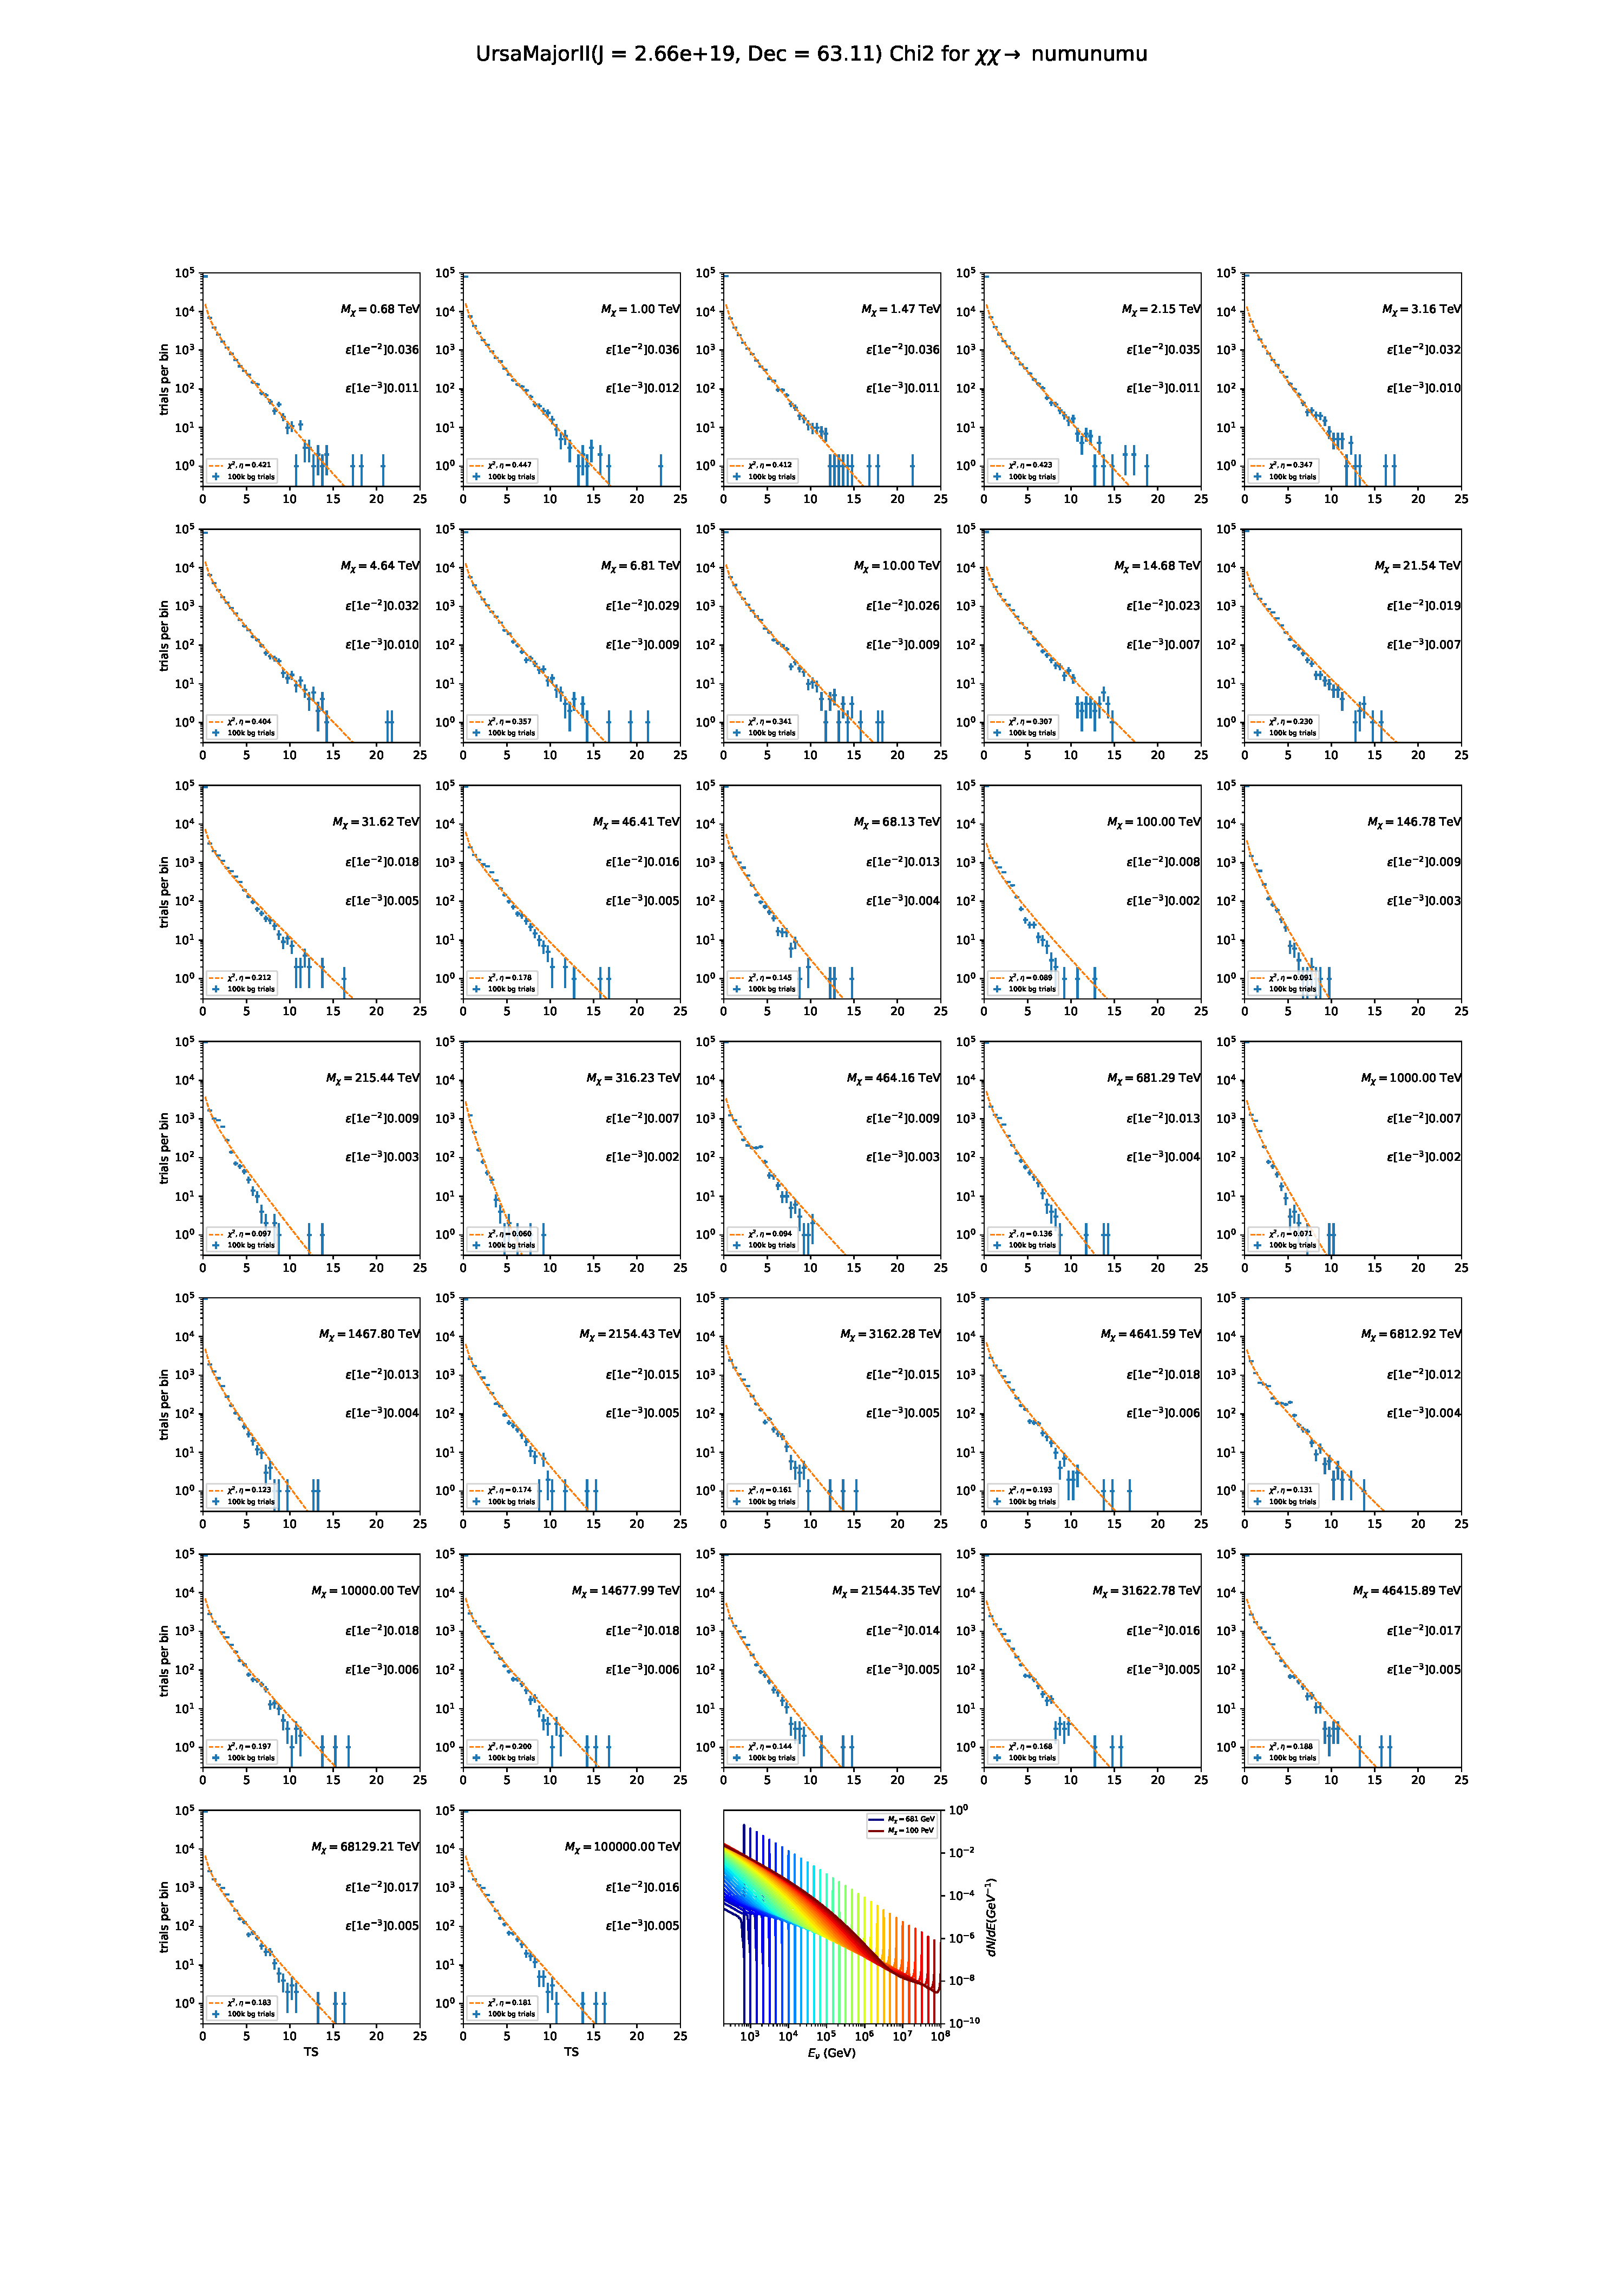
\includegraphics[clip, trim=5cm 6.5cm 4.9cm 8cm, scale=0.345]{figures/ic_DM/dm_plots/UrsaMajorII_numunumu_chi2_Masspanel_2024-03-23.pdf}
    }\caption{Same as \cref{fig:icDM_Seg1bb_TS} for Ursa Major II 1 $\chi\chi \rightarrow$ \parpar{\nu_\mu}.}
    \label{fig:icDM_UMa2numu_TS}
\end{figure}


%%%%%%%%%%%%%%%%%%%%%%%%%%%%%%%%%%%%%%%%%%%%%%%%%%
\subsection{Stacked TS} \label{sec:icDM_TSstacked}
%%%%%%%%%%%%%%%%%%%%%%%%%%%%%%%%%%%%%%%%%%%%%%%%%%

\begin{figure}[ht]
    \centering{
        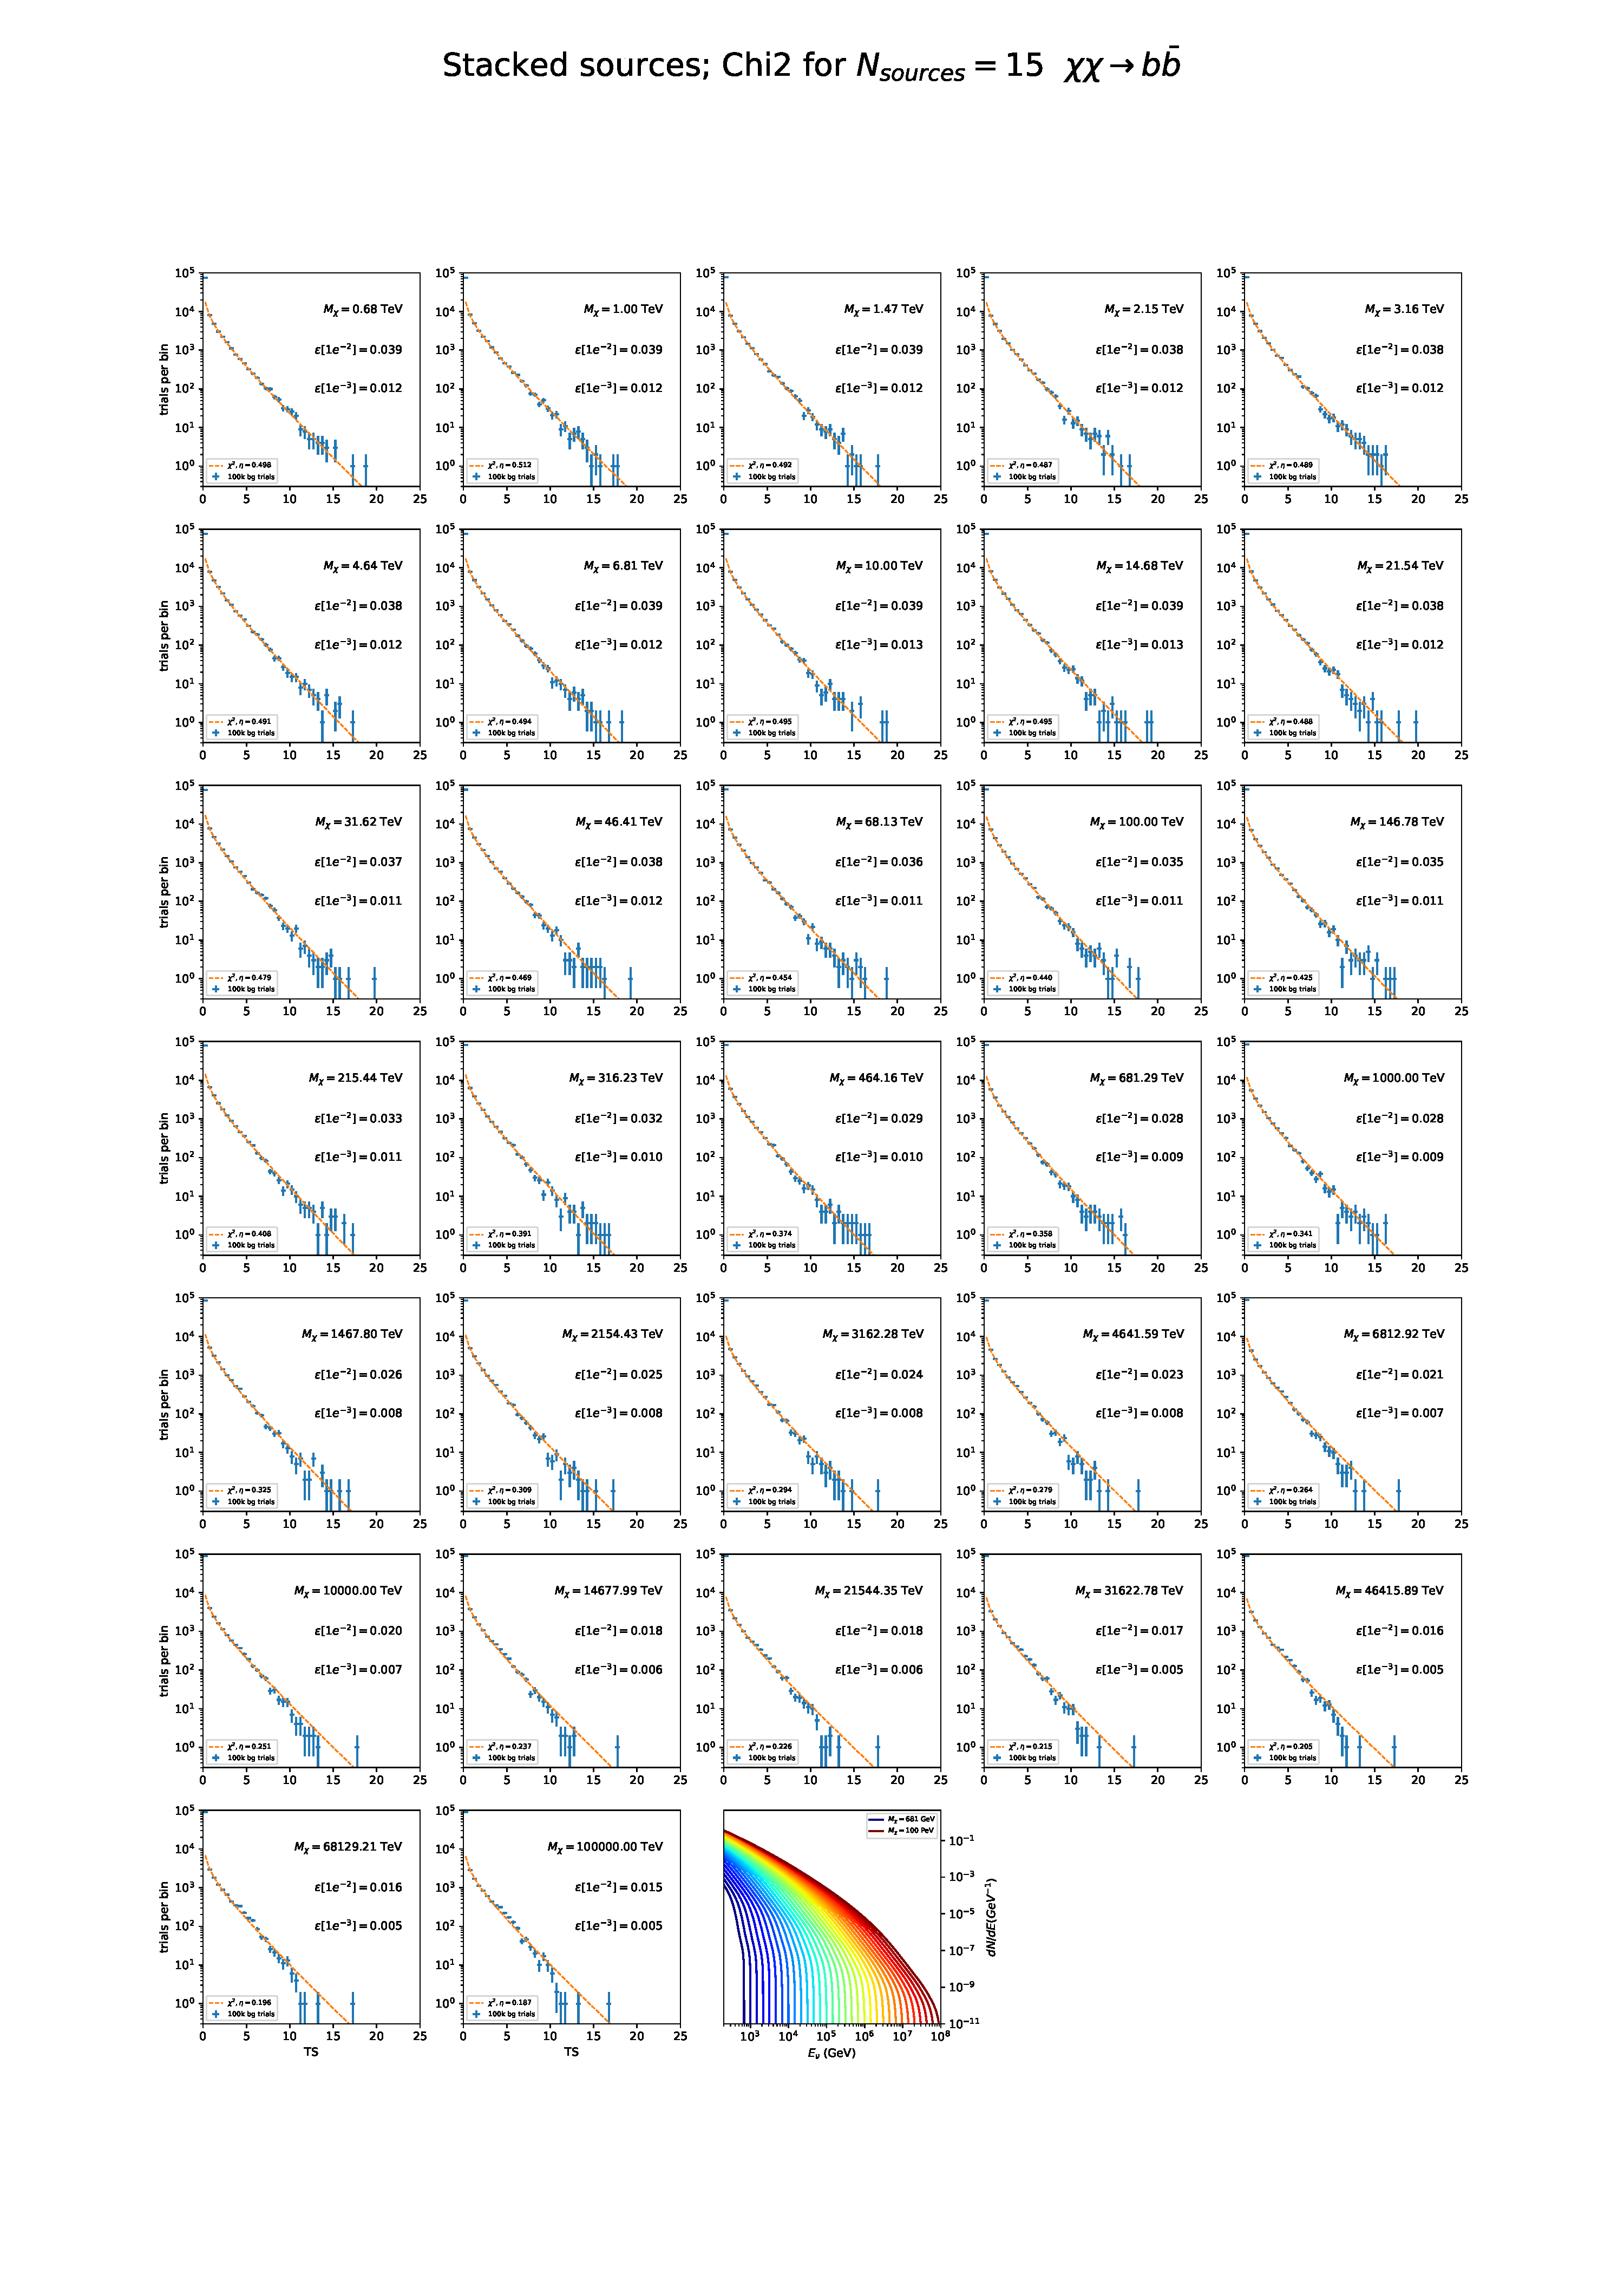
\includegraphics[clip, trim=5cm 6.5cm 4.9cm 8cm, scale=0.345]{figures/ic_DM/dm_plots/stacked_bb_chi2_Masspanel_2024-03-23.pdf}
    }\caption{Same as \cref{fig:icDM_Seg1bb_TS} for 15, \GS \J-factor, stacked sources and $\chi\chi \rightarrow$ \parpar{b}.}
    \label{fig:icDM_stact_bb_TS}
\end{figure}

\begin{figure}[ht]
    \centering{
        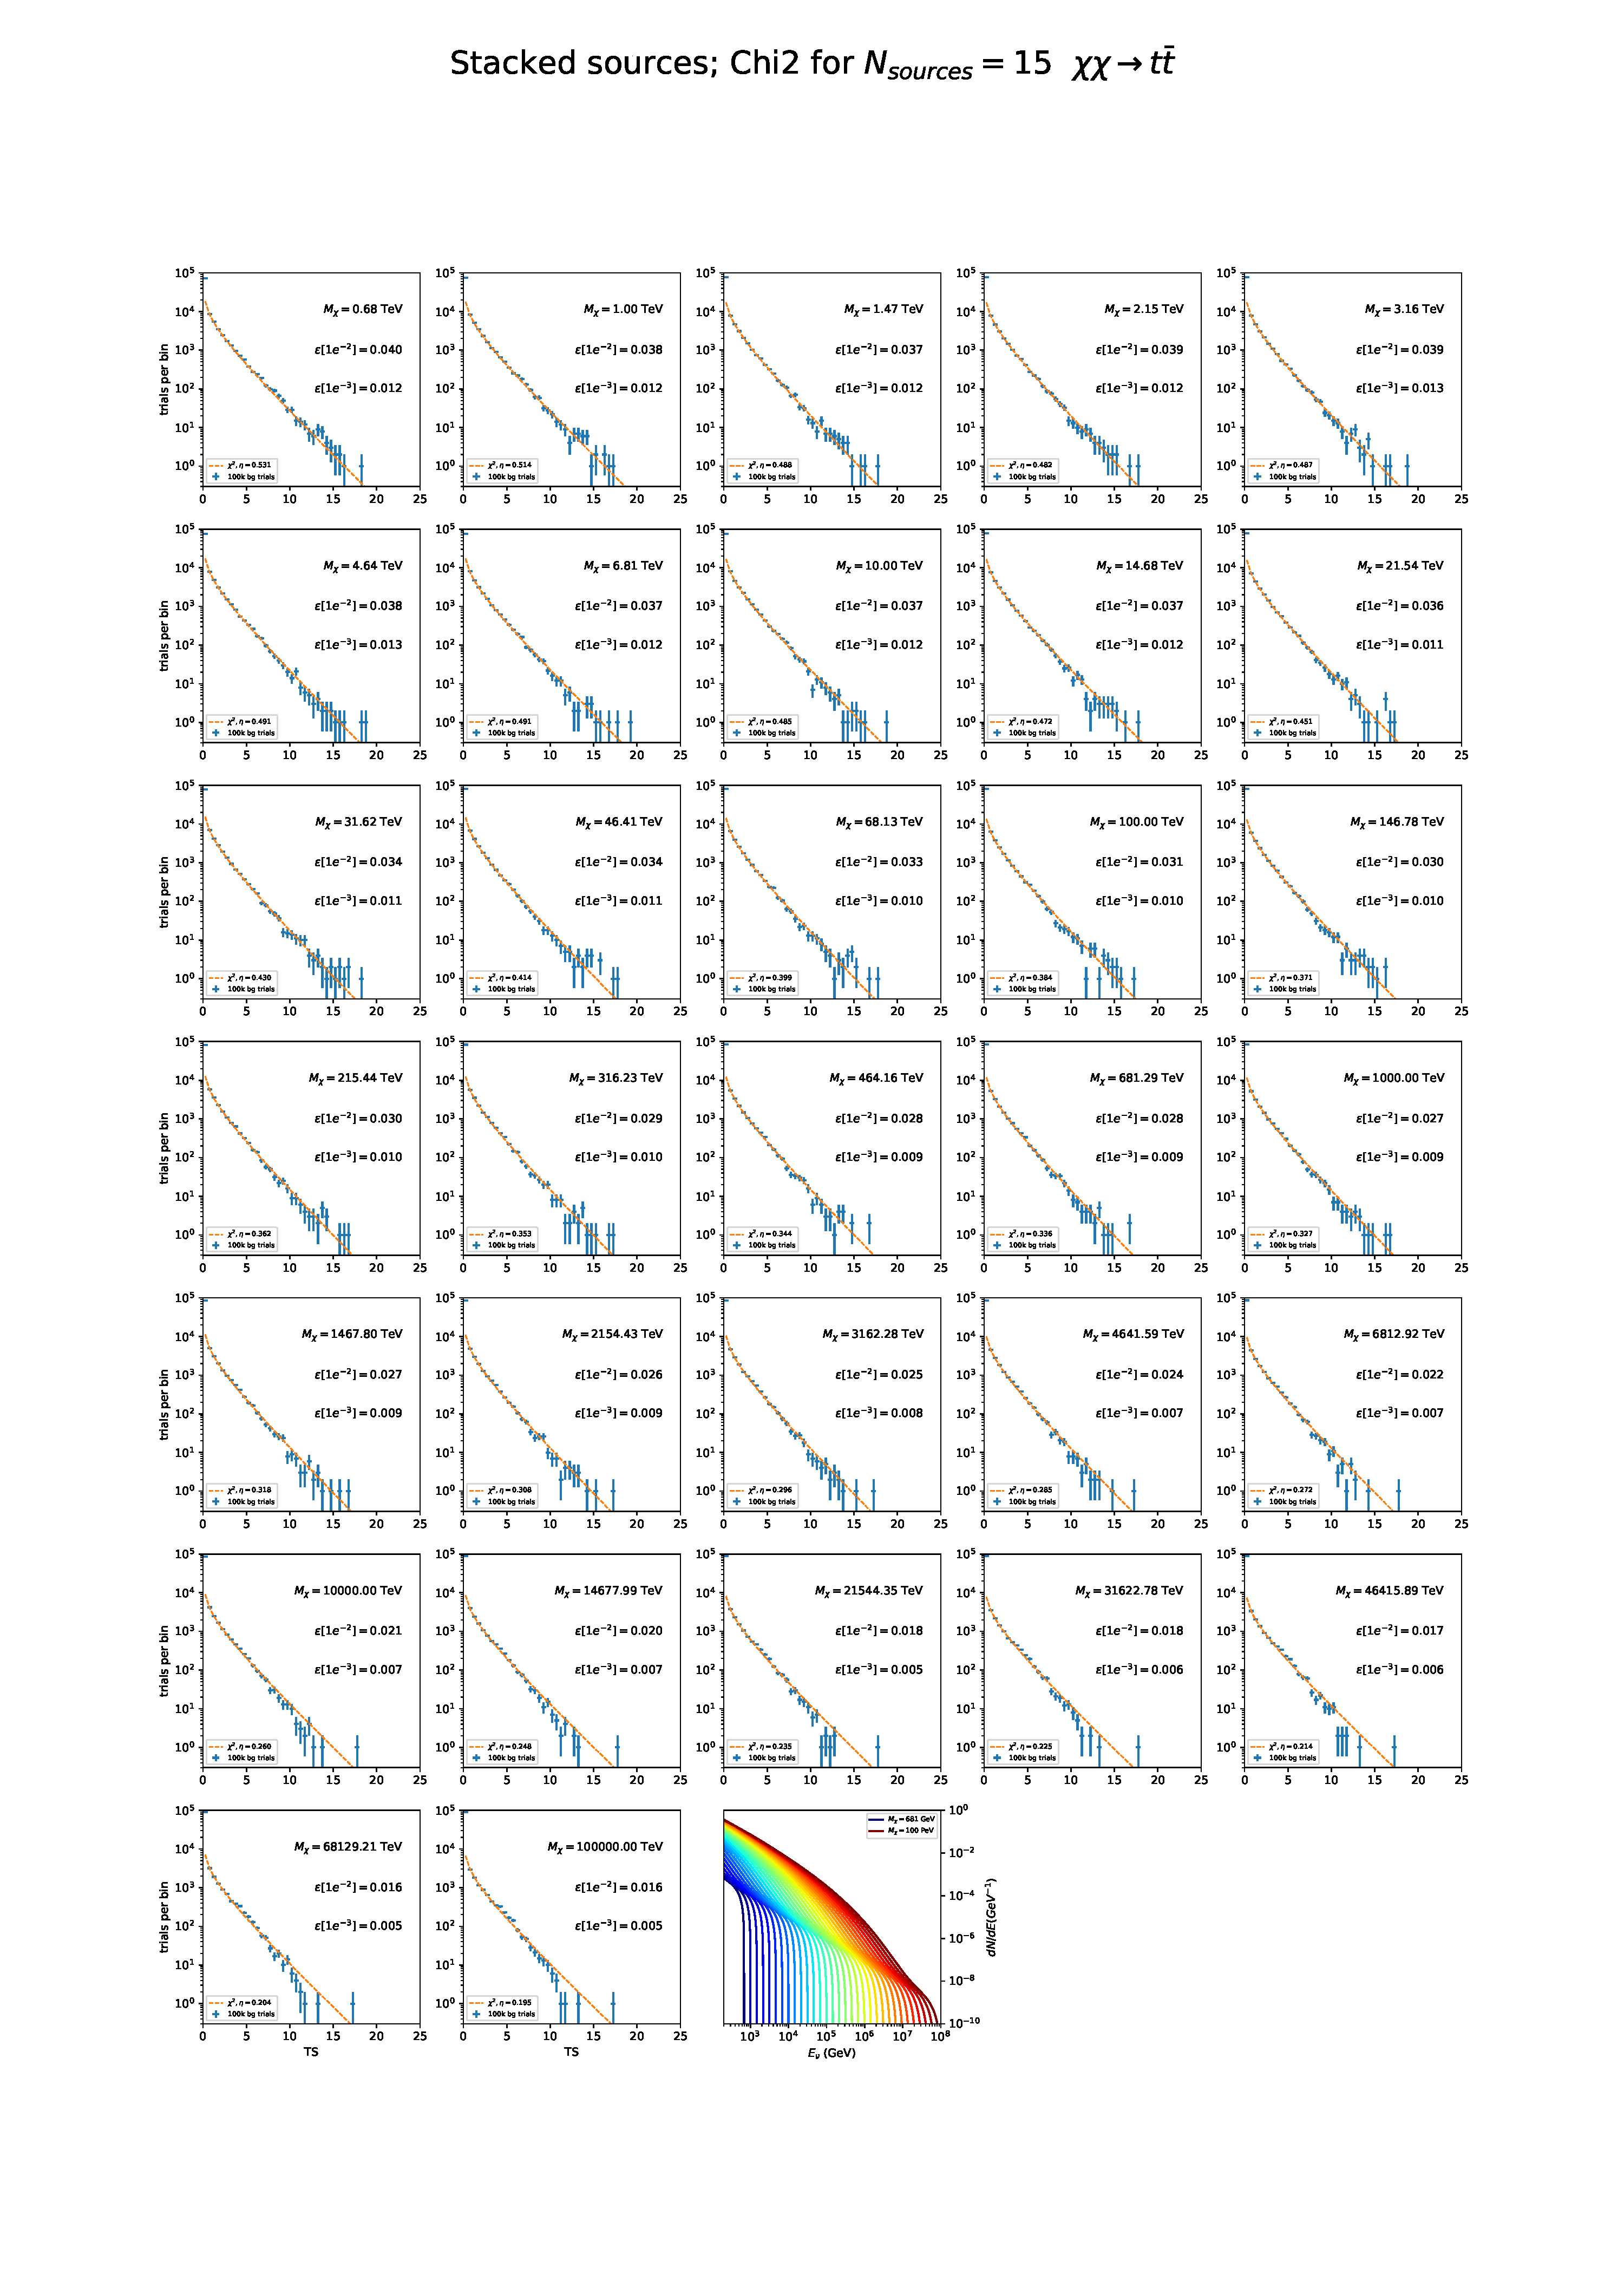
\includegraphics[clip, trim=5cm 6.5cm 4.9cm 8cm, scale=0.345]{figures/ic_DM/dm_plots/stacked_tt_chi2_Masspanel_2024-03-23.pdf}
    }\caption{Same as \cref{fig:icDM_Seg1bb_TS} for 15, \GS \J-factor, stacked sources and $\chi\chi \rightarrow$ \parpar{t}.}
    \label{fig:icDM_stact_tt_TS}
\end{figure}

\begin{figure}[ht]
    \centering{
        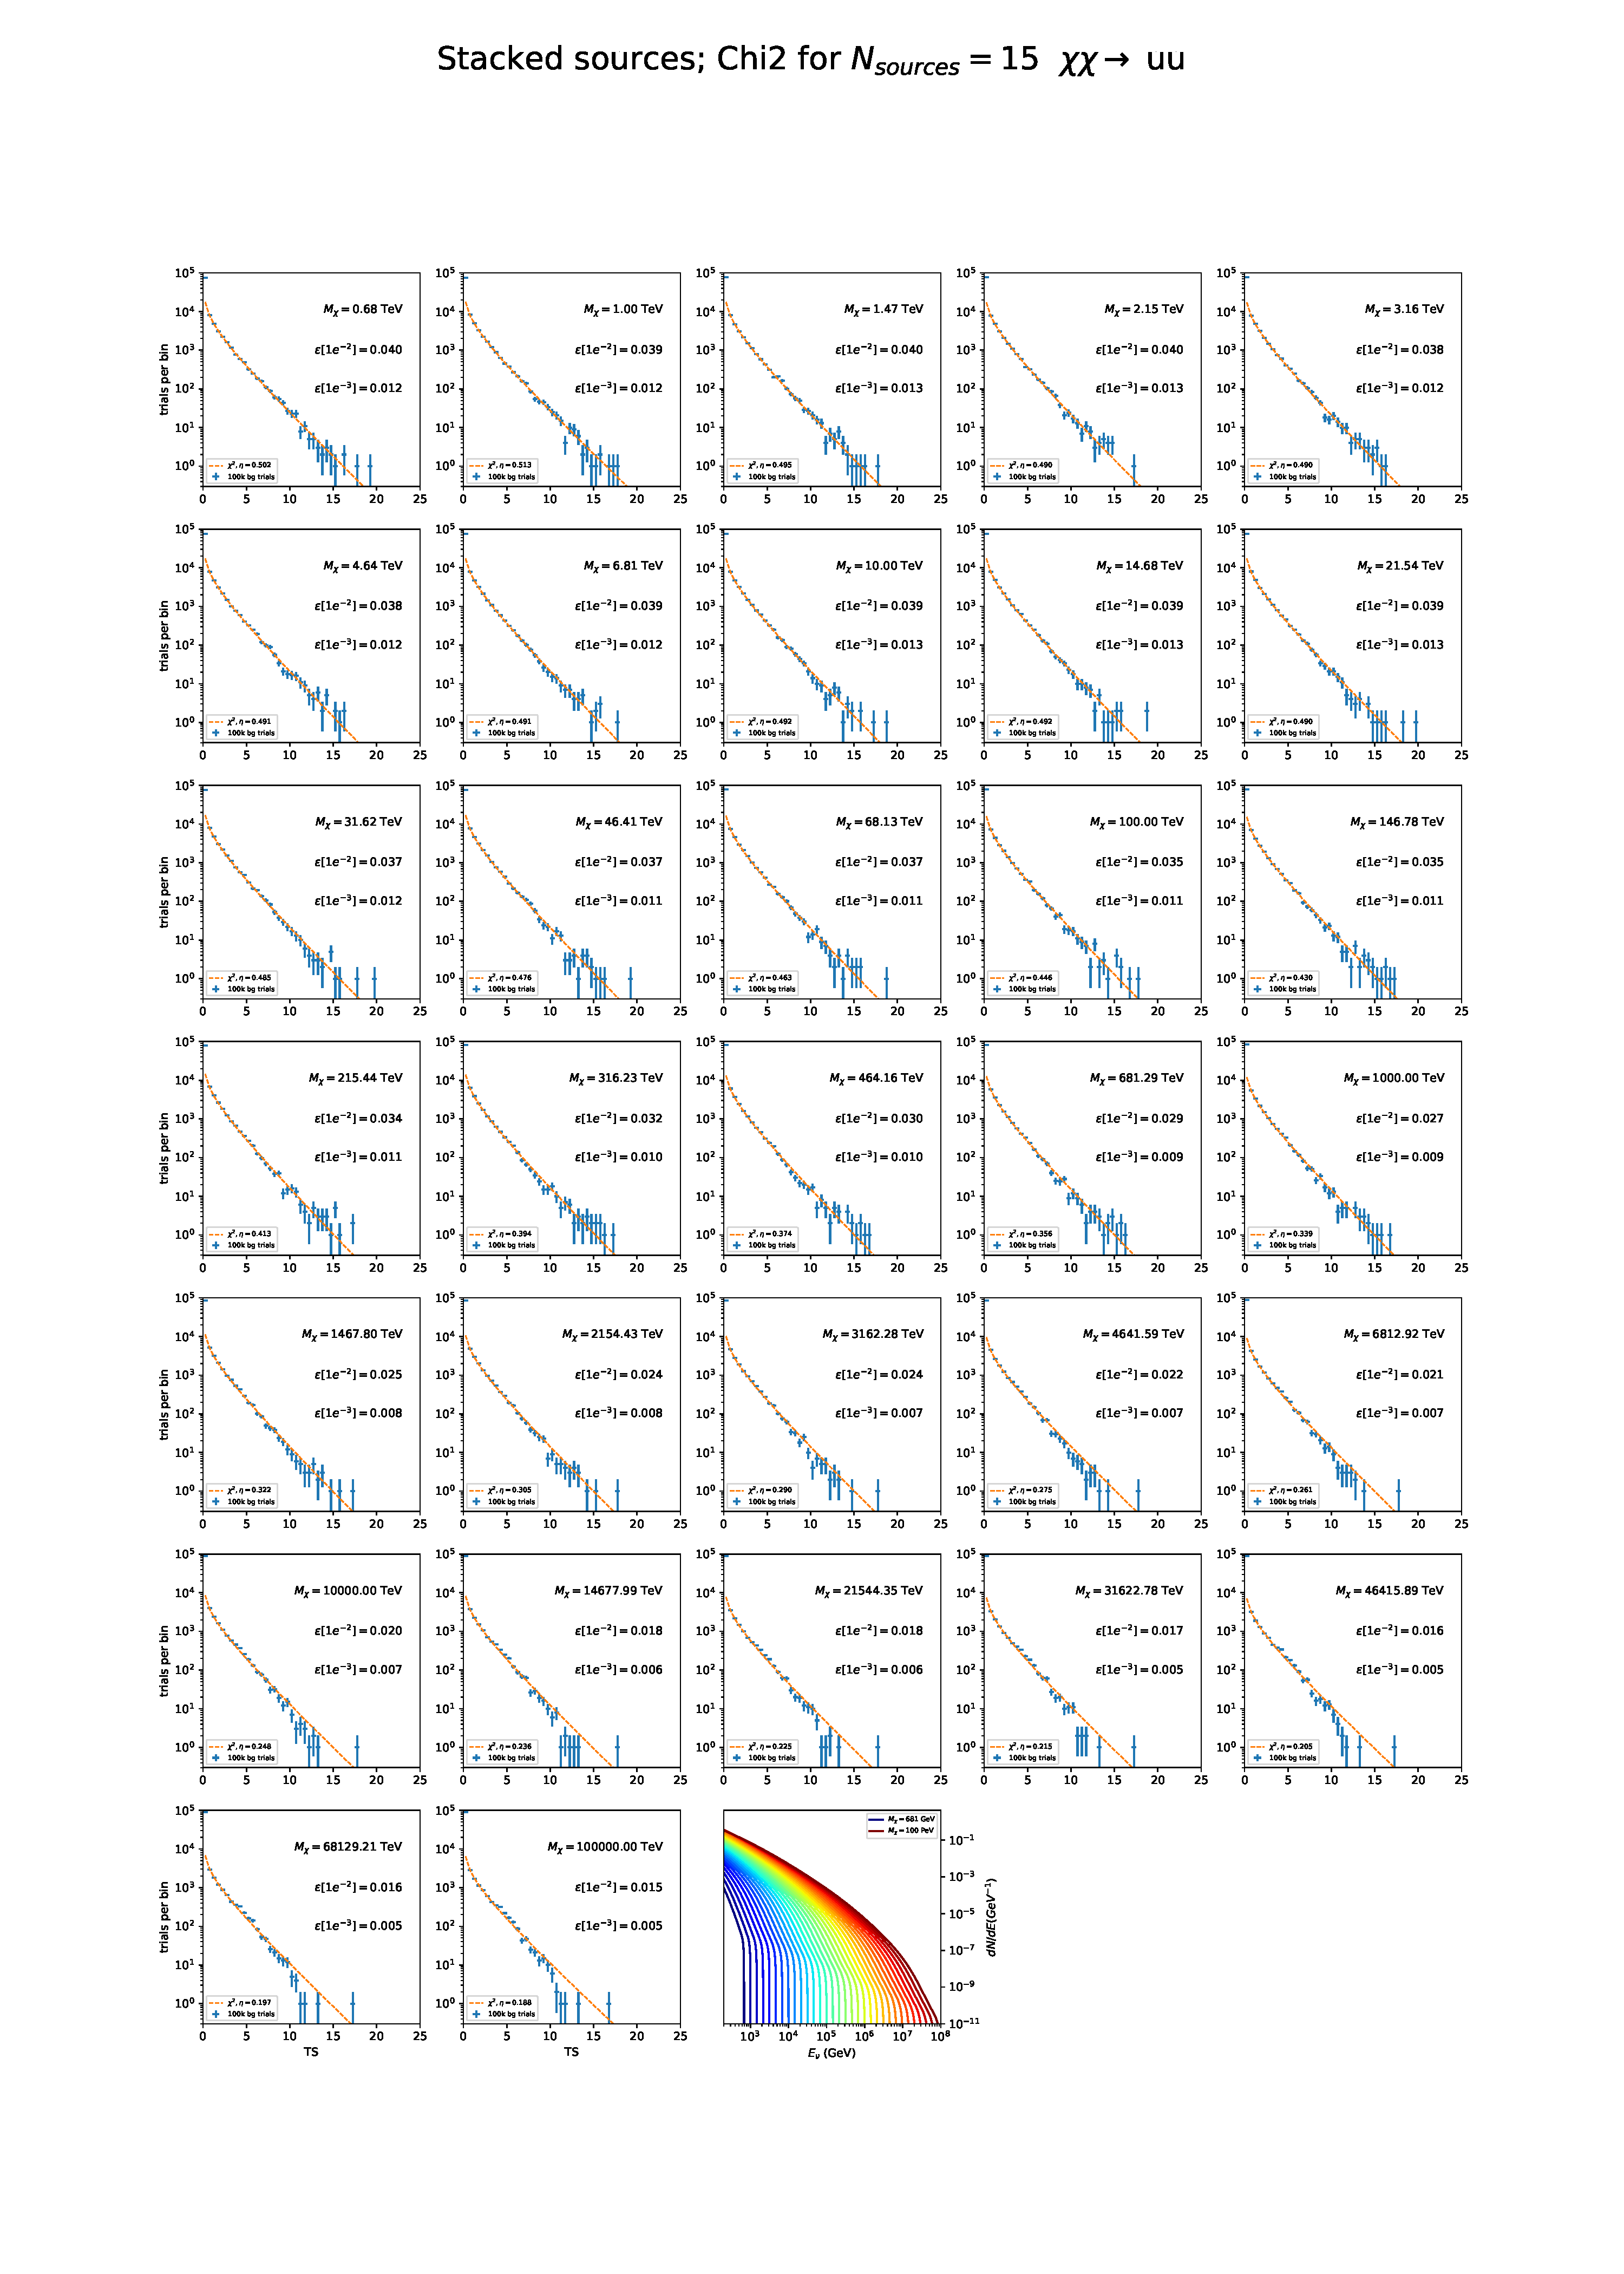
\includegraphics[clip, trim=5cm 6.5cm 4.9cm 8cm, scale=0.345]{figures/ic_DM/dm_plots/stacked_uu_chi2_Masspanel_2024-03-23.pdf}
    }\caption{Same as \cref{fig:icDM_Seg1bb_TS} for 15, \GS \J-factor, stacked sources and $\chi\chi \rightarrow$ \parpar{u}.}
    \label{fig:icDM_stact_uu_TS}
\end{figure}

\begin{figure}[ht]
    \centering{
        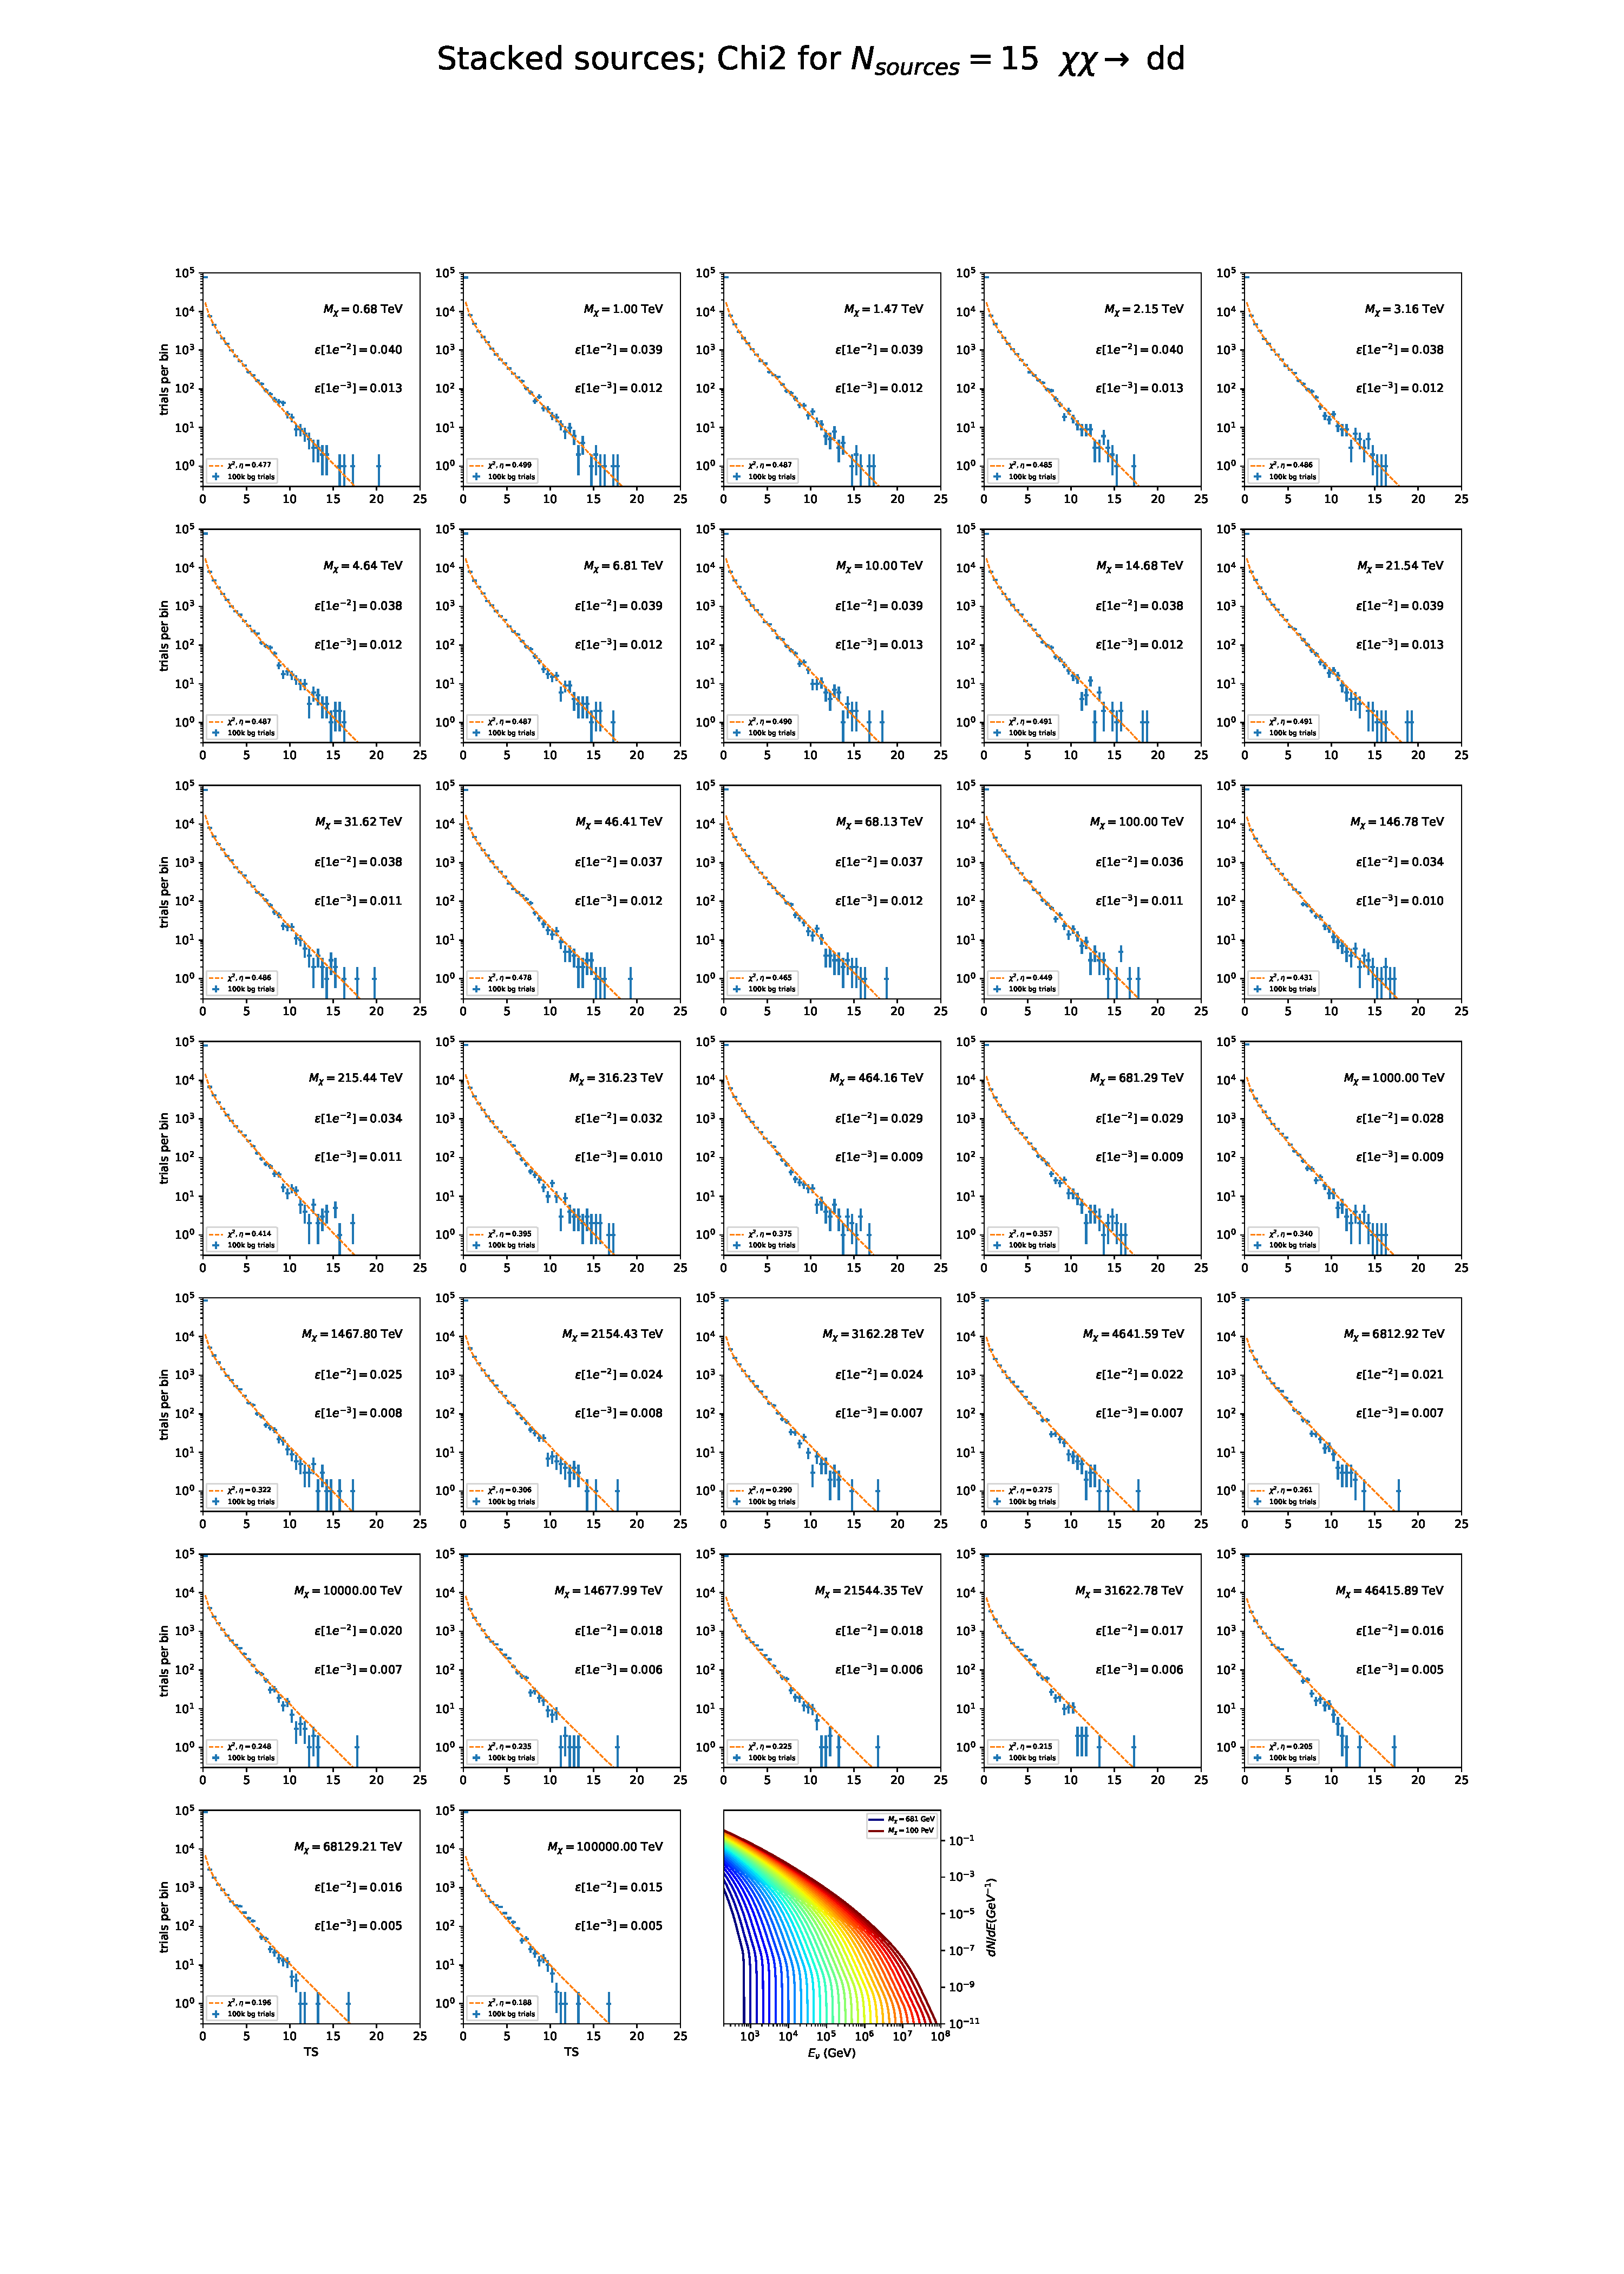
\includegraphics[clip, trim=5cm 6.5cm 4.9cm 8cm, scale=0.345]{figures/ic_DM/dm_plots/stacked_dd_chi2_Masspanel_2024-03-23.pdf}
    }\caption{Same as \cref{fig:icDM_Seg1bb_TS} for 15, \GS \J-factor, stacked sources and $\chi\chi \rightarrow$ \parpar{d}.}
    \label{fig:icDM_stact_dd_TS}
\end{figure}

\begin{figure}[ht]
    \centering{
        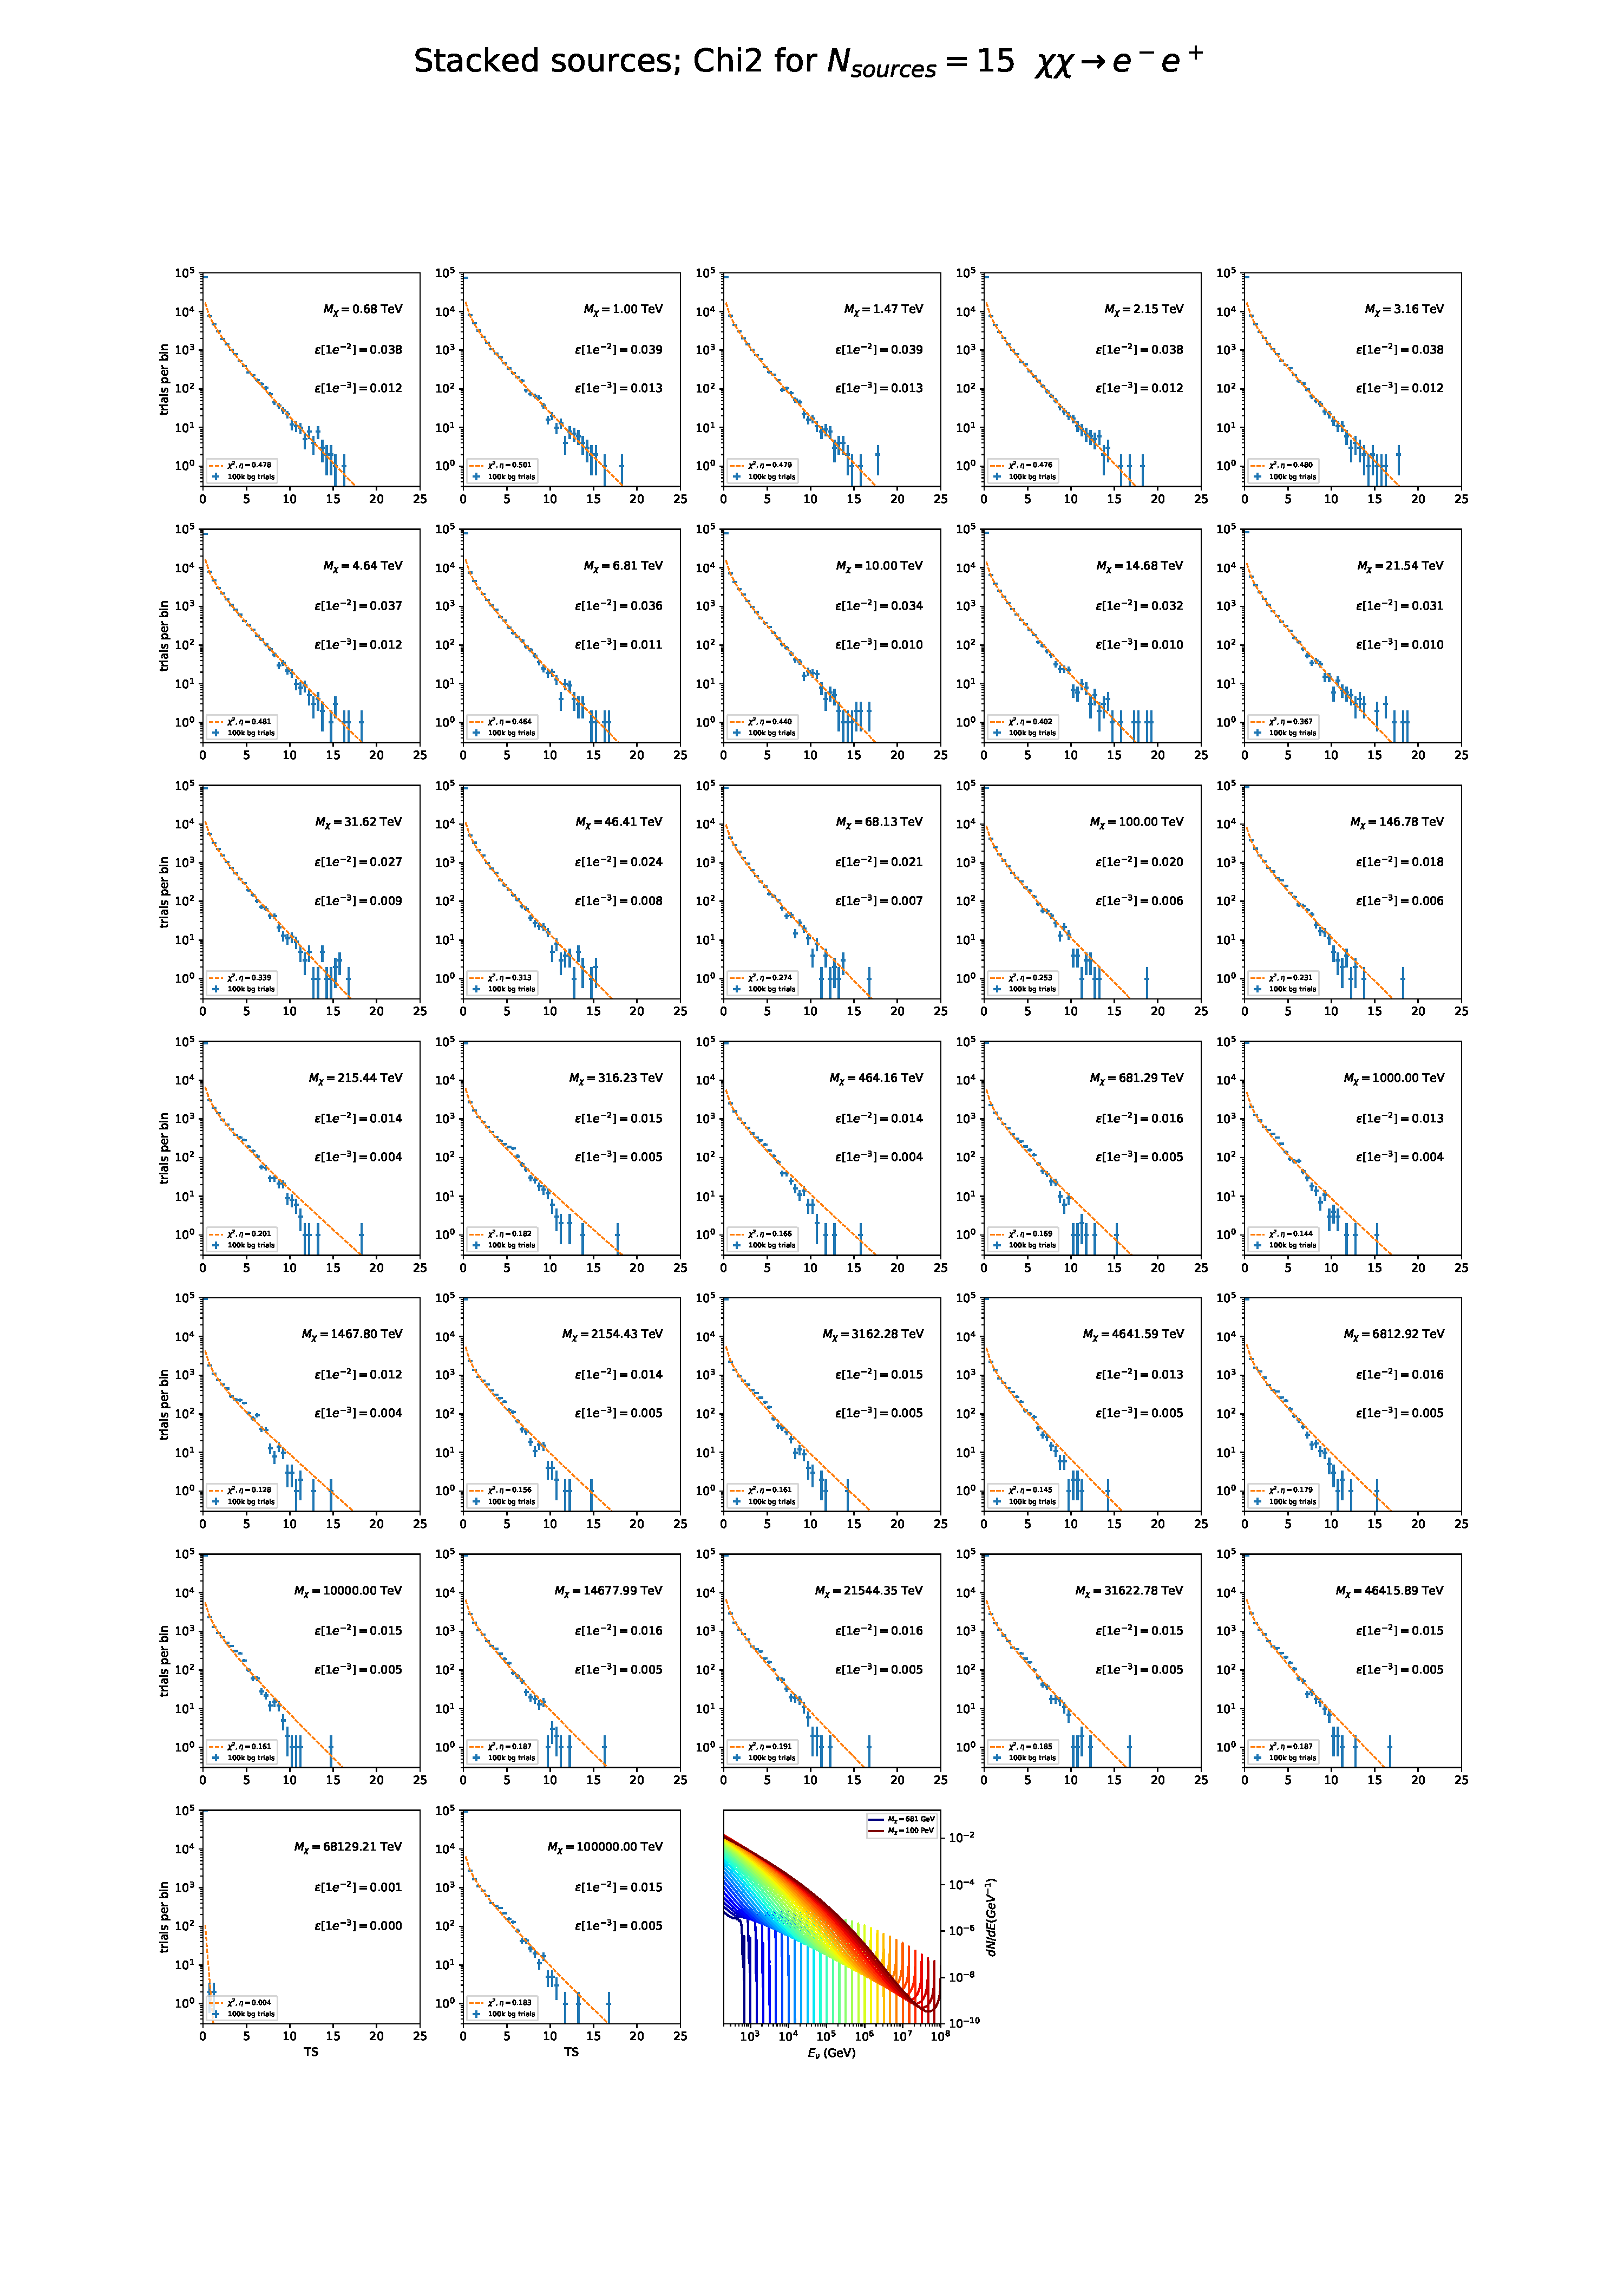
\includegraphics[clip, trim=5cm 6.5cm 4.9cm 8cm, scale=0.345]{figures/ic_DM/dm_plots/stacked_ee_chi2_Masspanel_2024-03-23.pdf}
    }\caption{Same as \cref{fig:icDM_Seg1bb_TS} for 15, \GS \J-factor, stacked sources and $\chi\chi \rightarrow$ \parpar{e}.}
    \label{fig:icDM_stact_ee_TS}
\end{figure}

\begin{figure}[ht]
    \centering{
        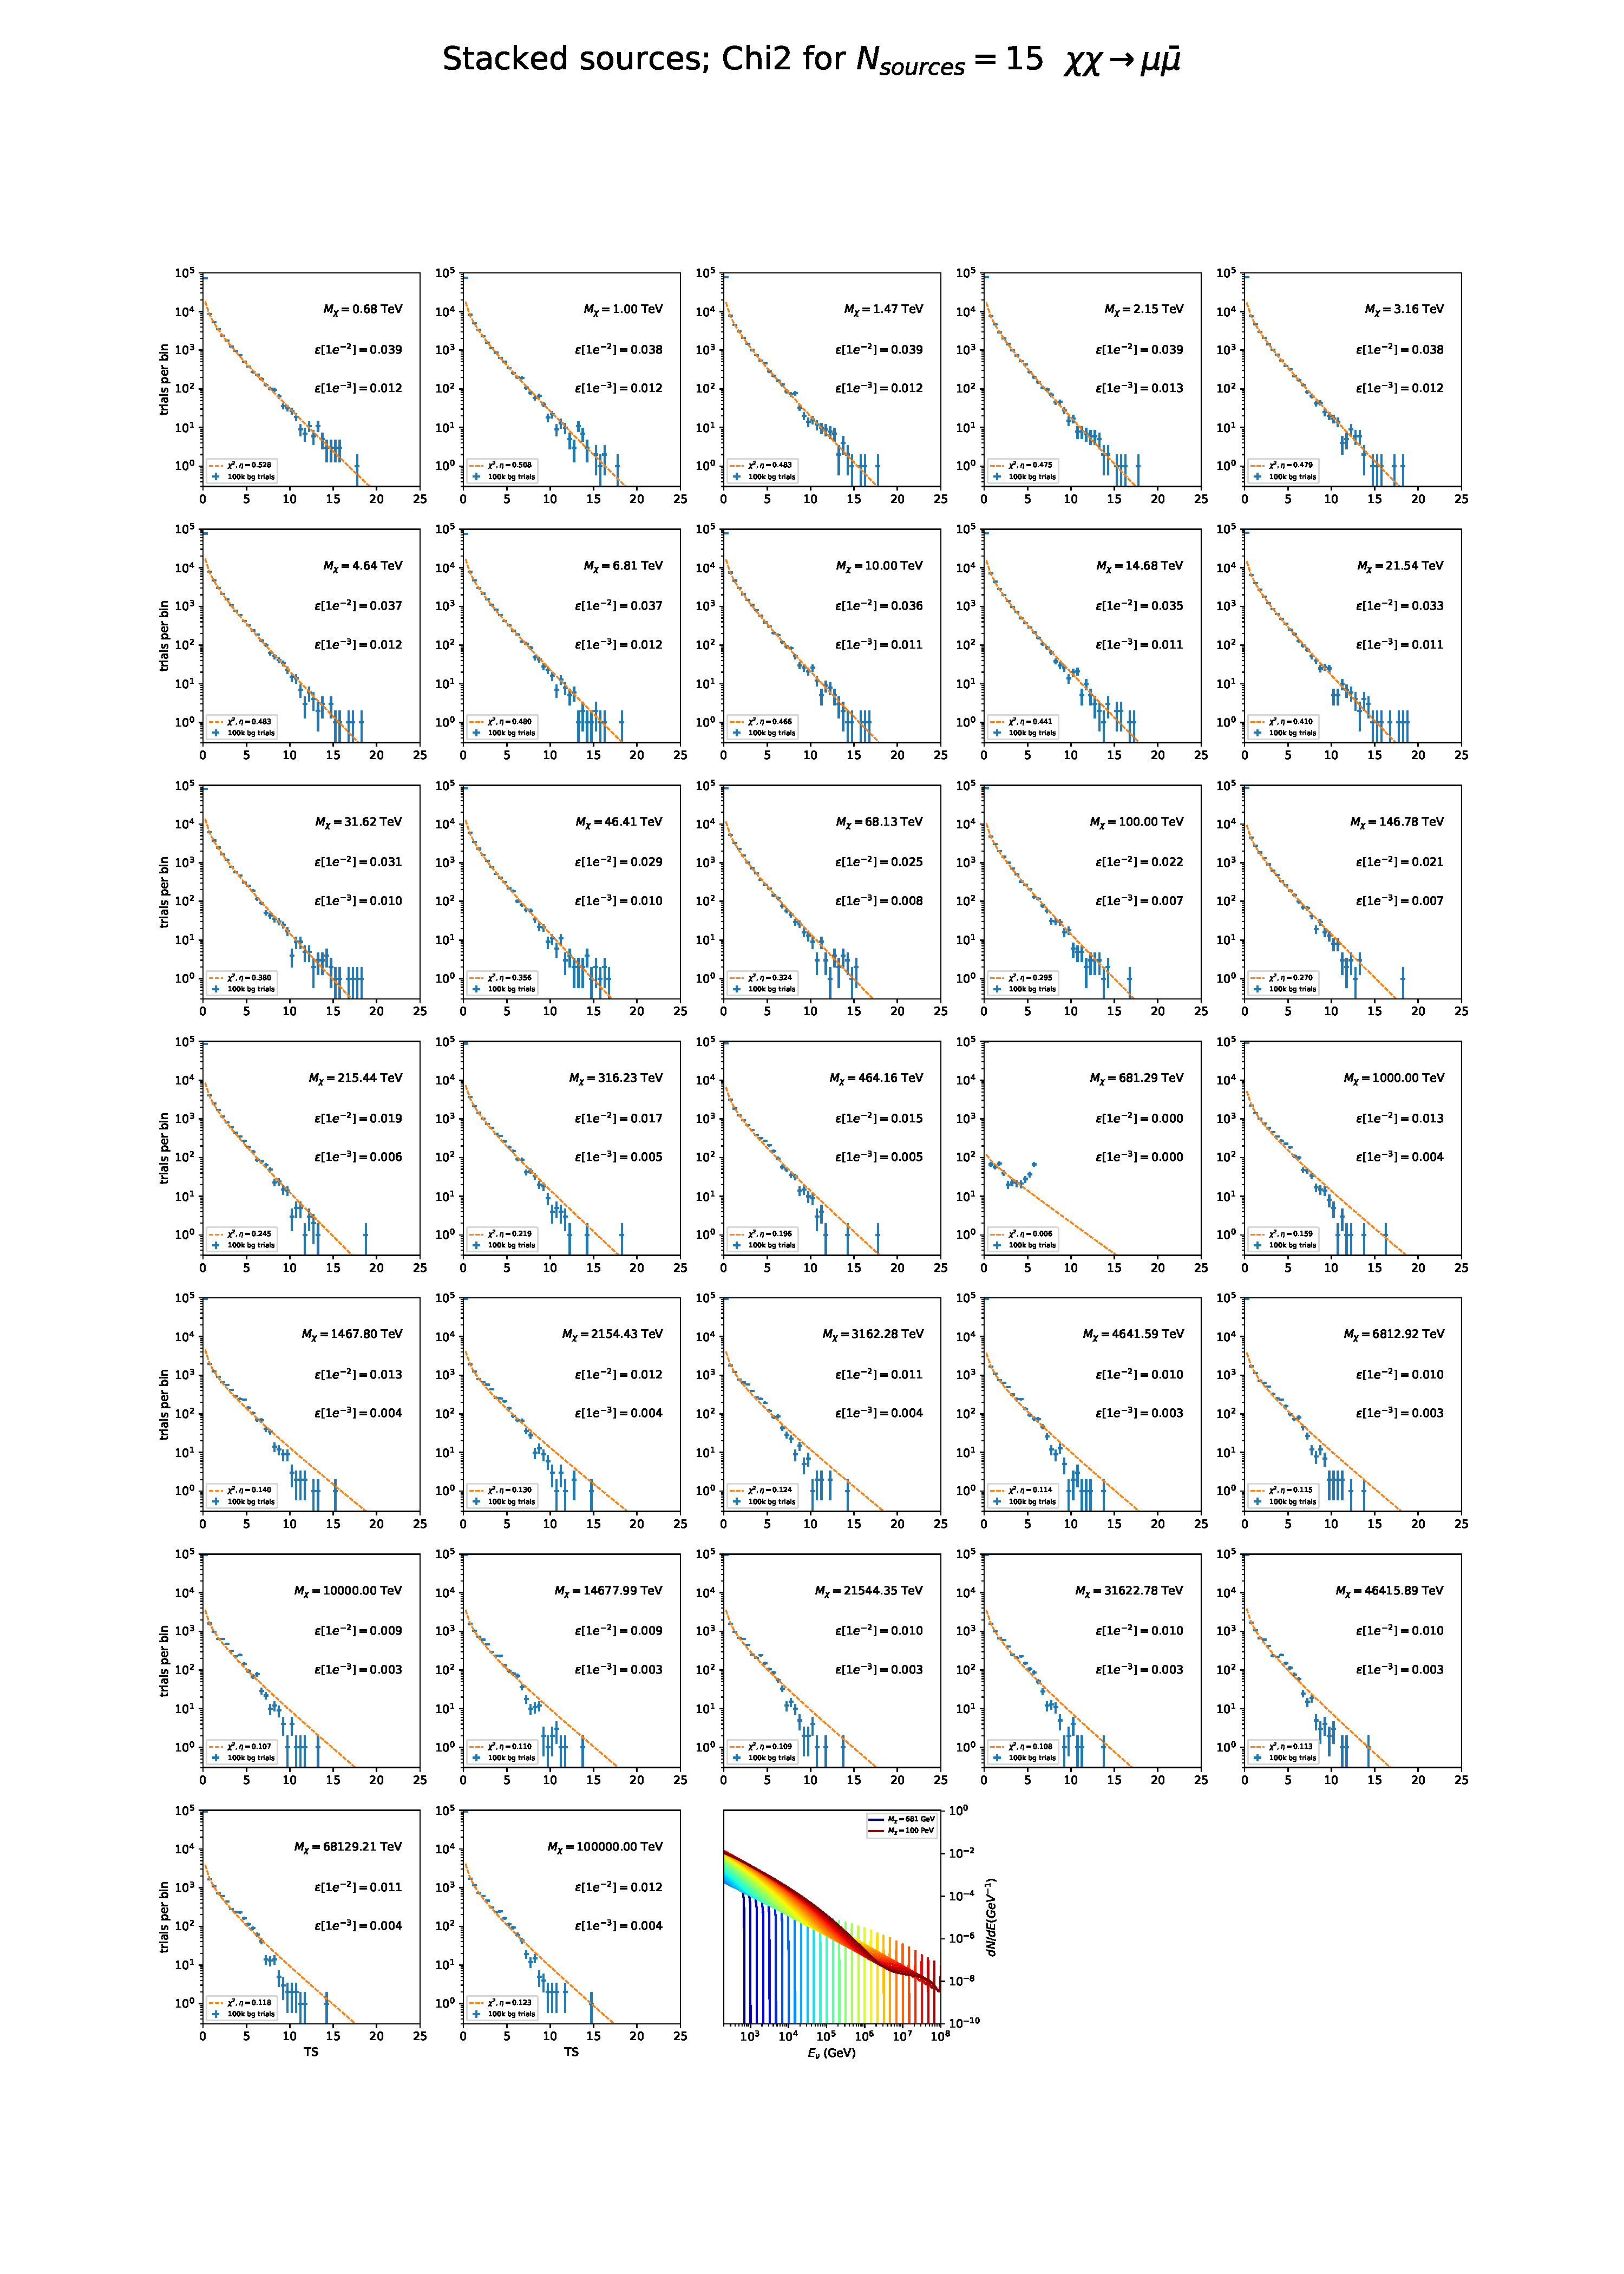
\includegraphics[clip, trim=5cm 6.5cm 4.9cm 8cm, scale=0.345]{figures/ic_DM/dm_plots/stacked_mumu_chi2_Masspanel_2024-03-23.pdf}
    }\caption{Same as \cref{fig:icDM_Seg1bb_TS} for 15, \GS \J-factor, stacked sources and $\chi\chi \rightarrow$ \parpar{\mu}.}
    \label{fig:icDM_stact_mu_TS}
\end{figure}

\begin{figure}[ht]
    \centering{
        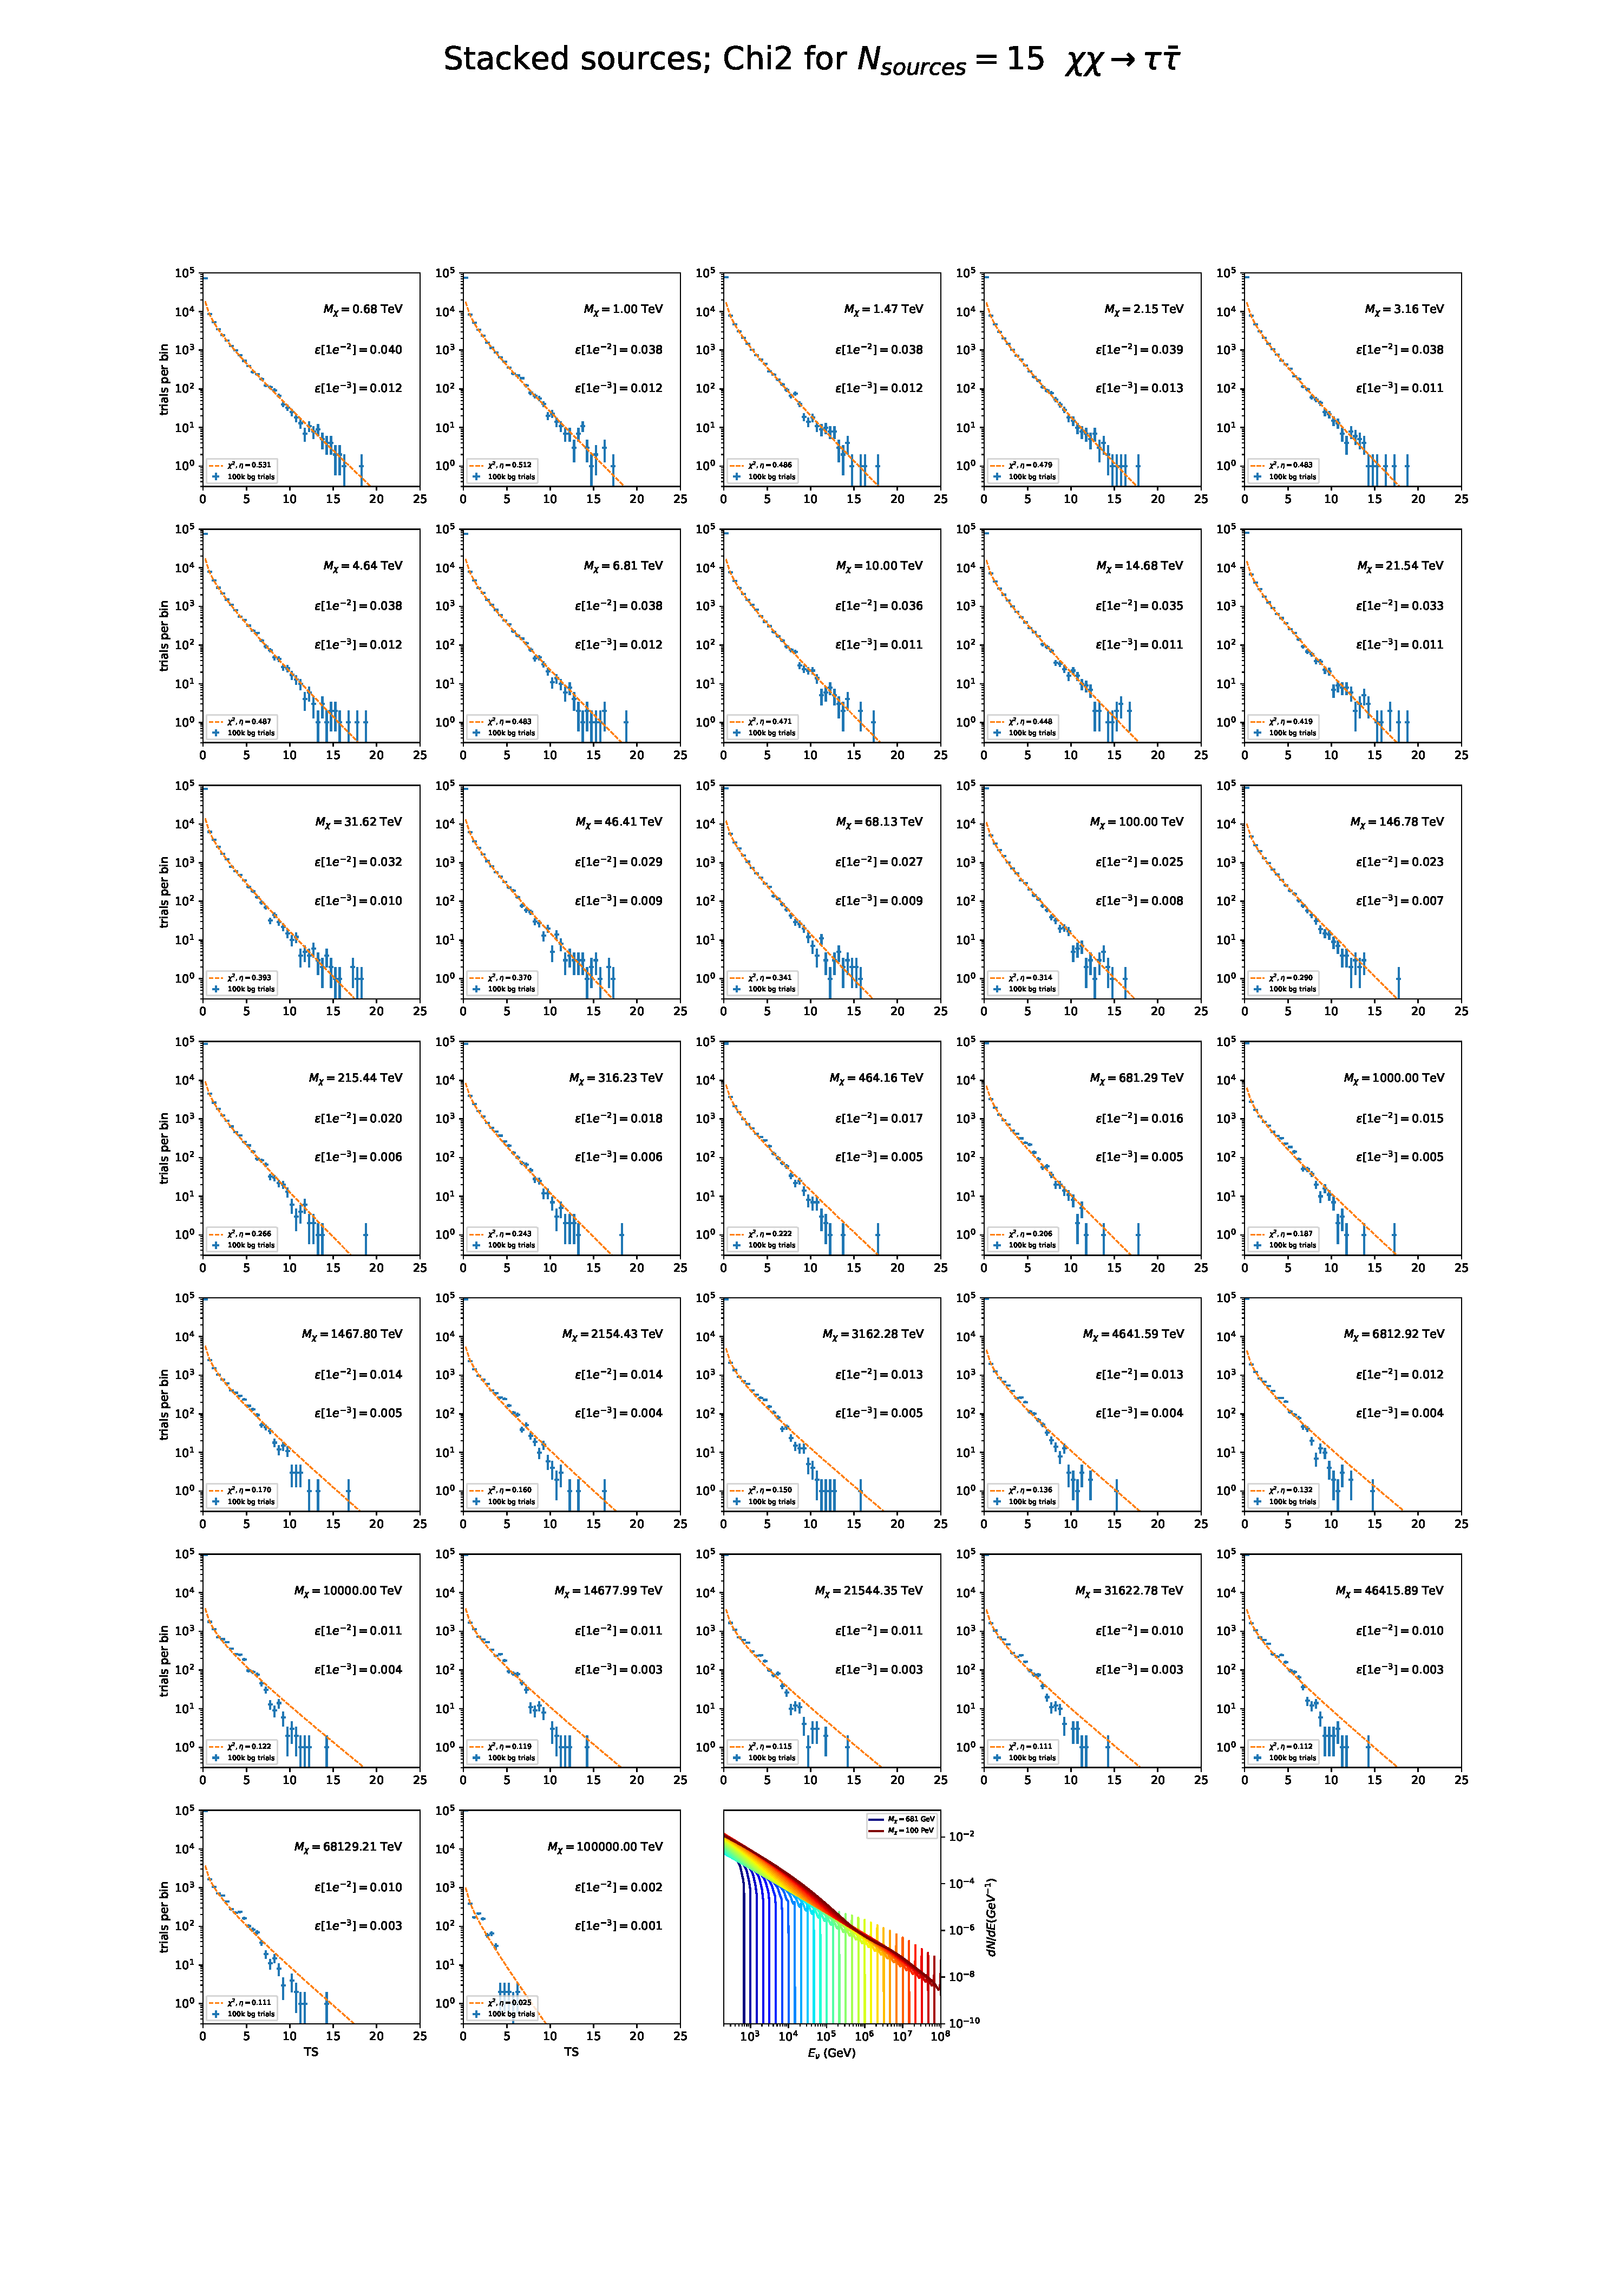
\includegraphics[clip, trim=5cm 6.5cm 4.9cm 8cm, scale=0.345]{figures/ic_DM/dm_plots/stacked_tautau_chi2_Masspanel_2024-03-23.pdf}
    }\caption{Same as \cref{fig:icDM_Seg1bb_TS} for 15, \GS \J-factor, stacked sources and $\chi\chi \rightarrow$ \parpar{\tau}.}
    \label{fig:icDM_stact_tau_TS}
\end{figure}

\begin{figure}[ht]
    \centering{
        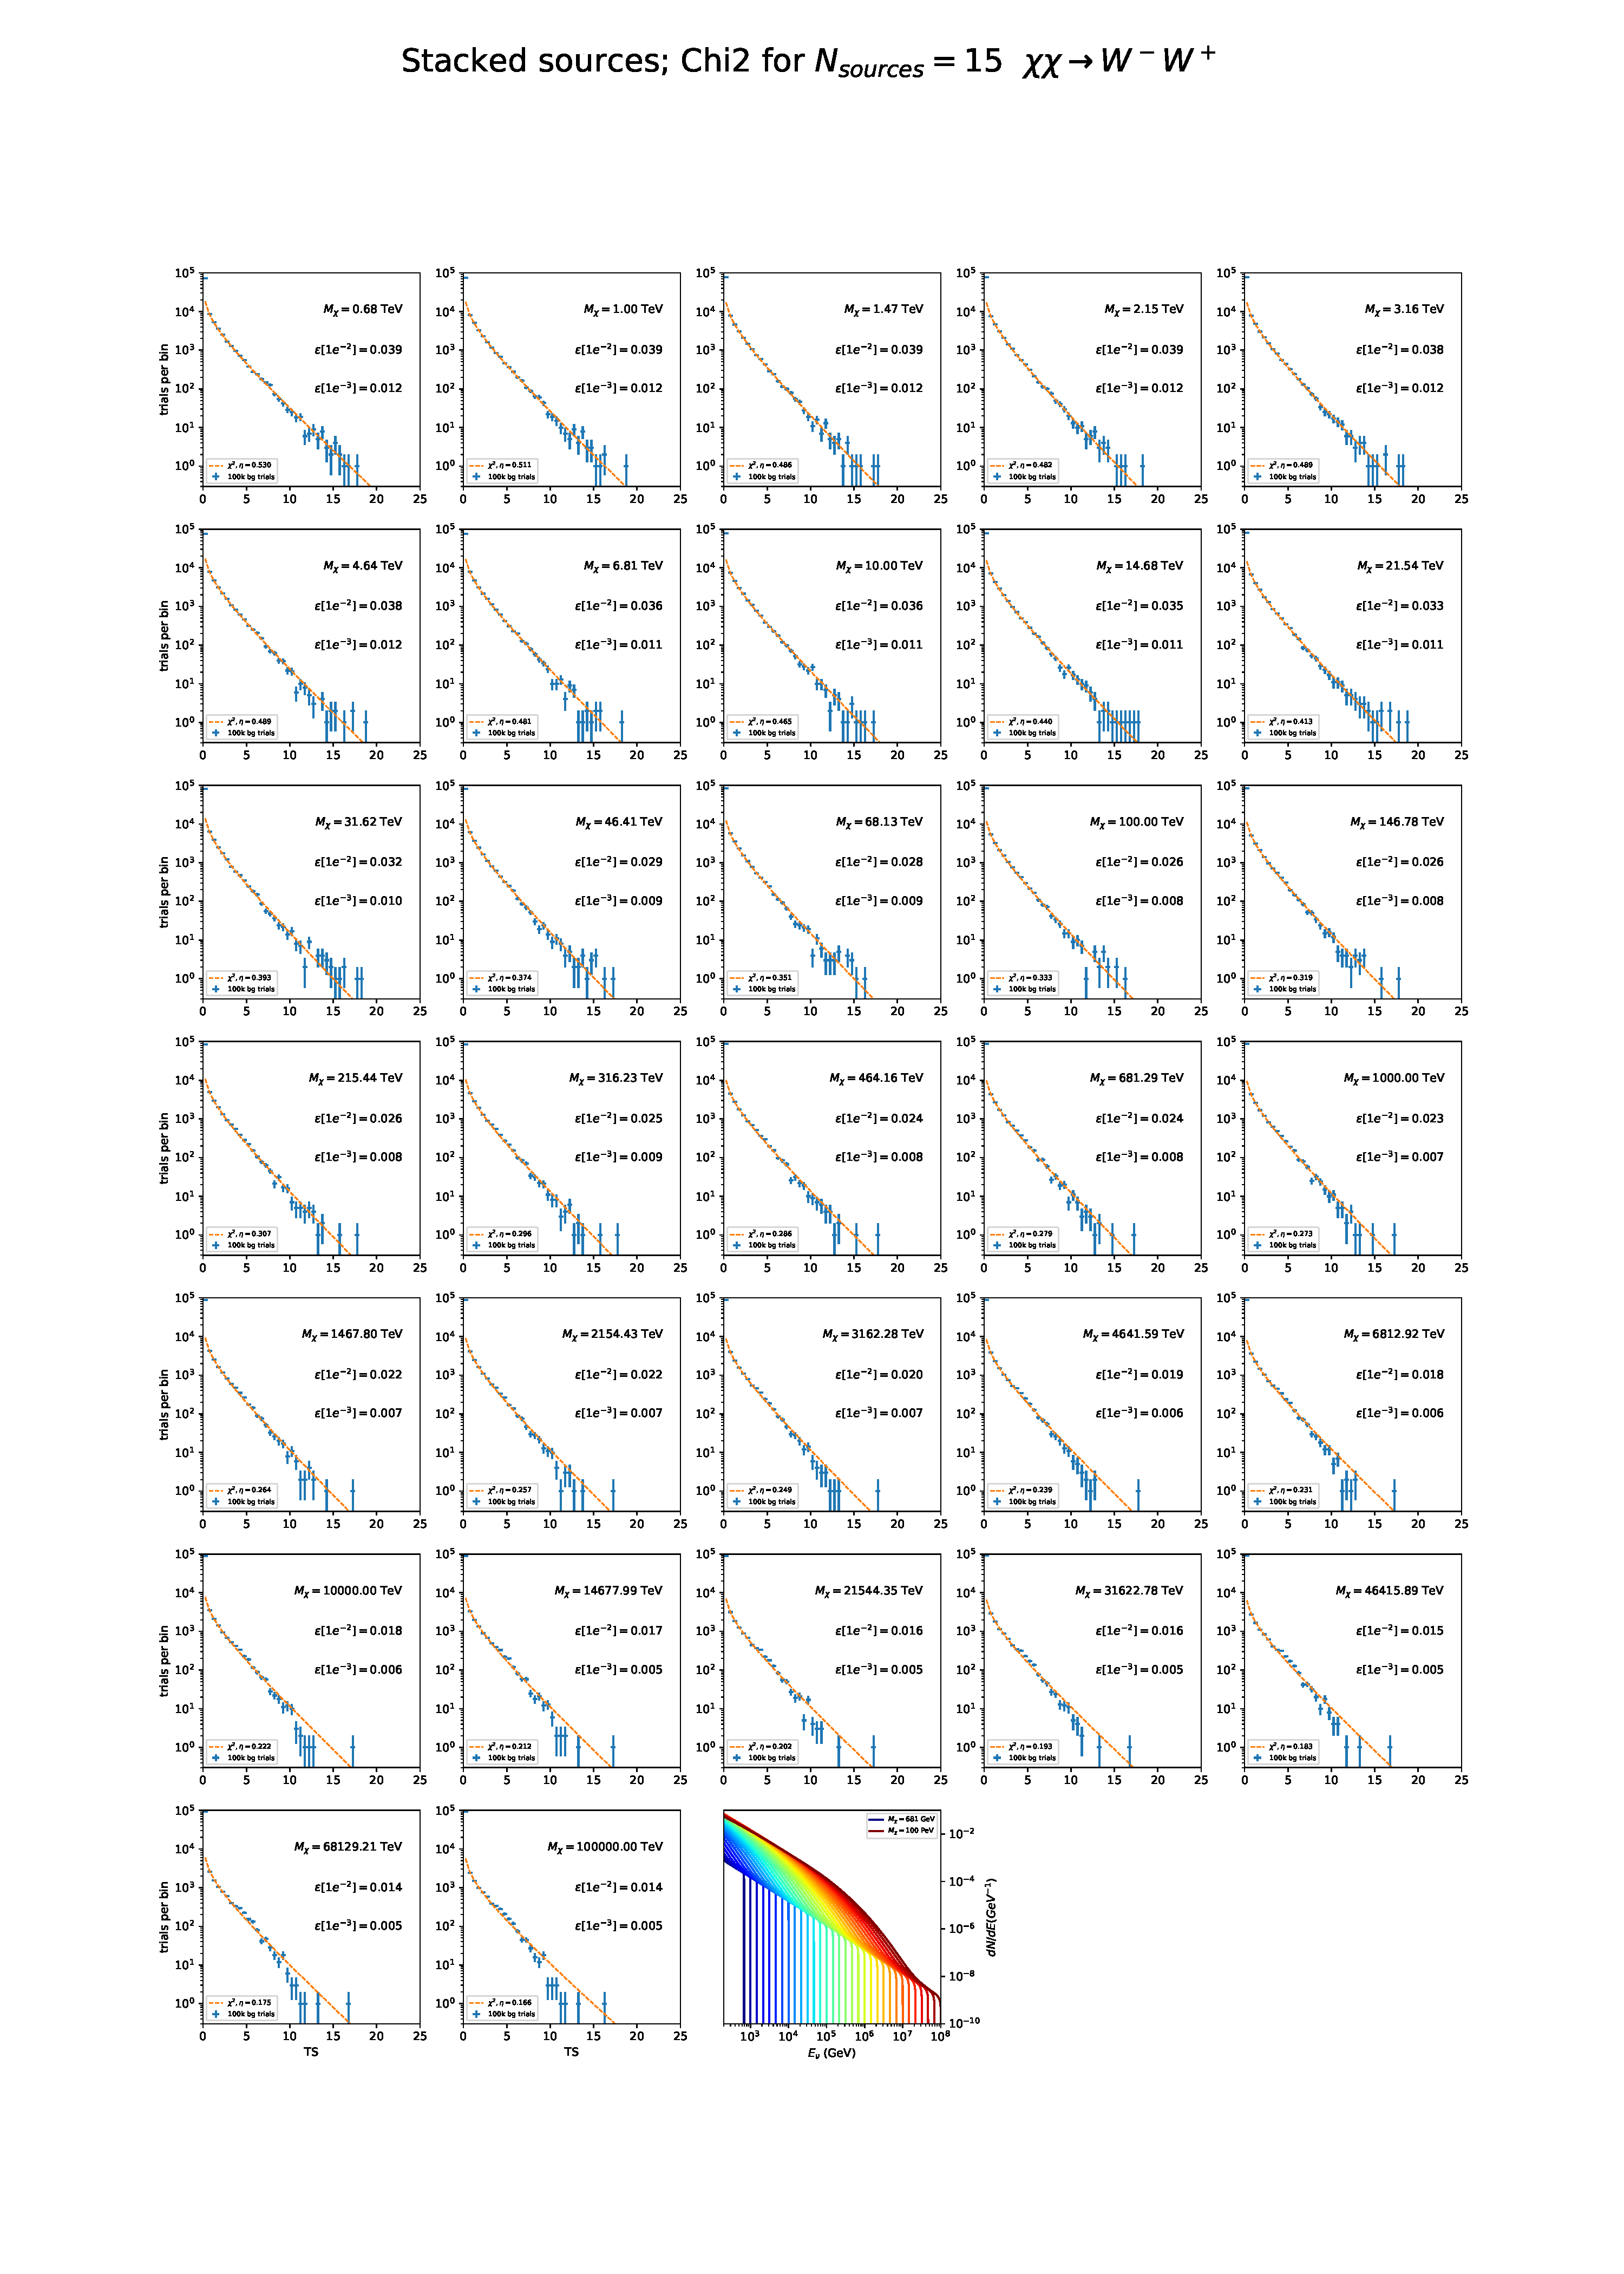
\includegraphics[clip, trim=5cm 6.5cm 4.9cm 8cm, scale=0.345]{figures/ic_DM/dm_plots/stacked_WW_chi2_Masspanel_2024-03-23.pdf}
    }\caption{Same as \cref{fig:icDM_Seg1bb_TS} for 15, \GS \J-factor, stacked sources and $\chi\chi \rightarrow$ $W^+W^-$.}
    \label{fig:icDM_stact_ww_TS}
\end{figure}

\begin{figure}[ht]
    \centering{
        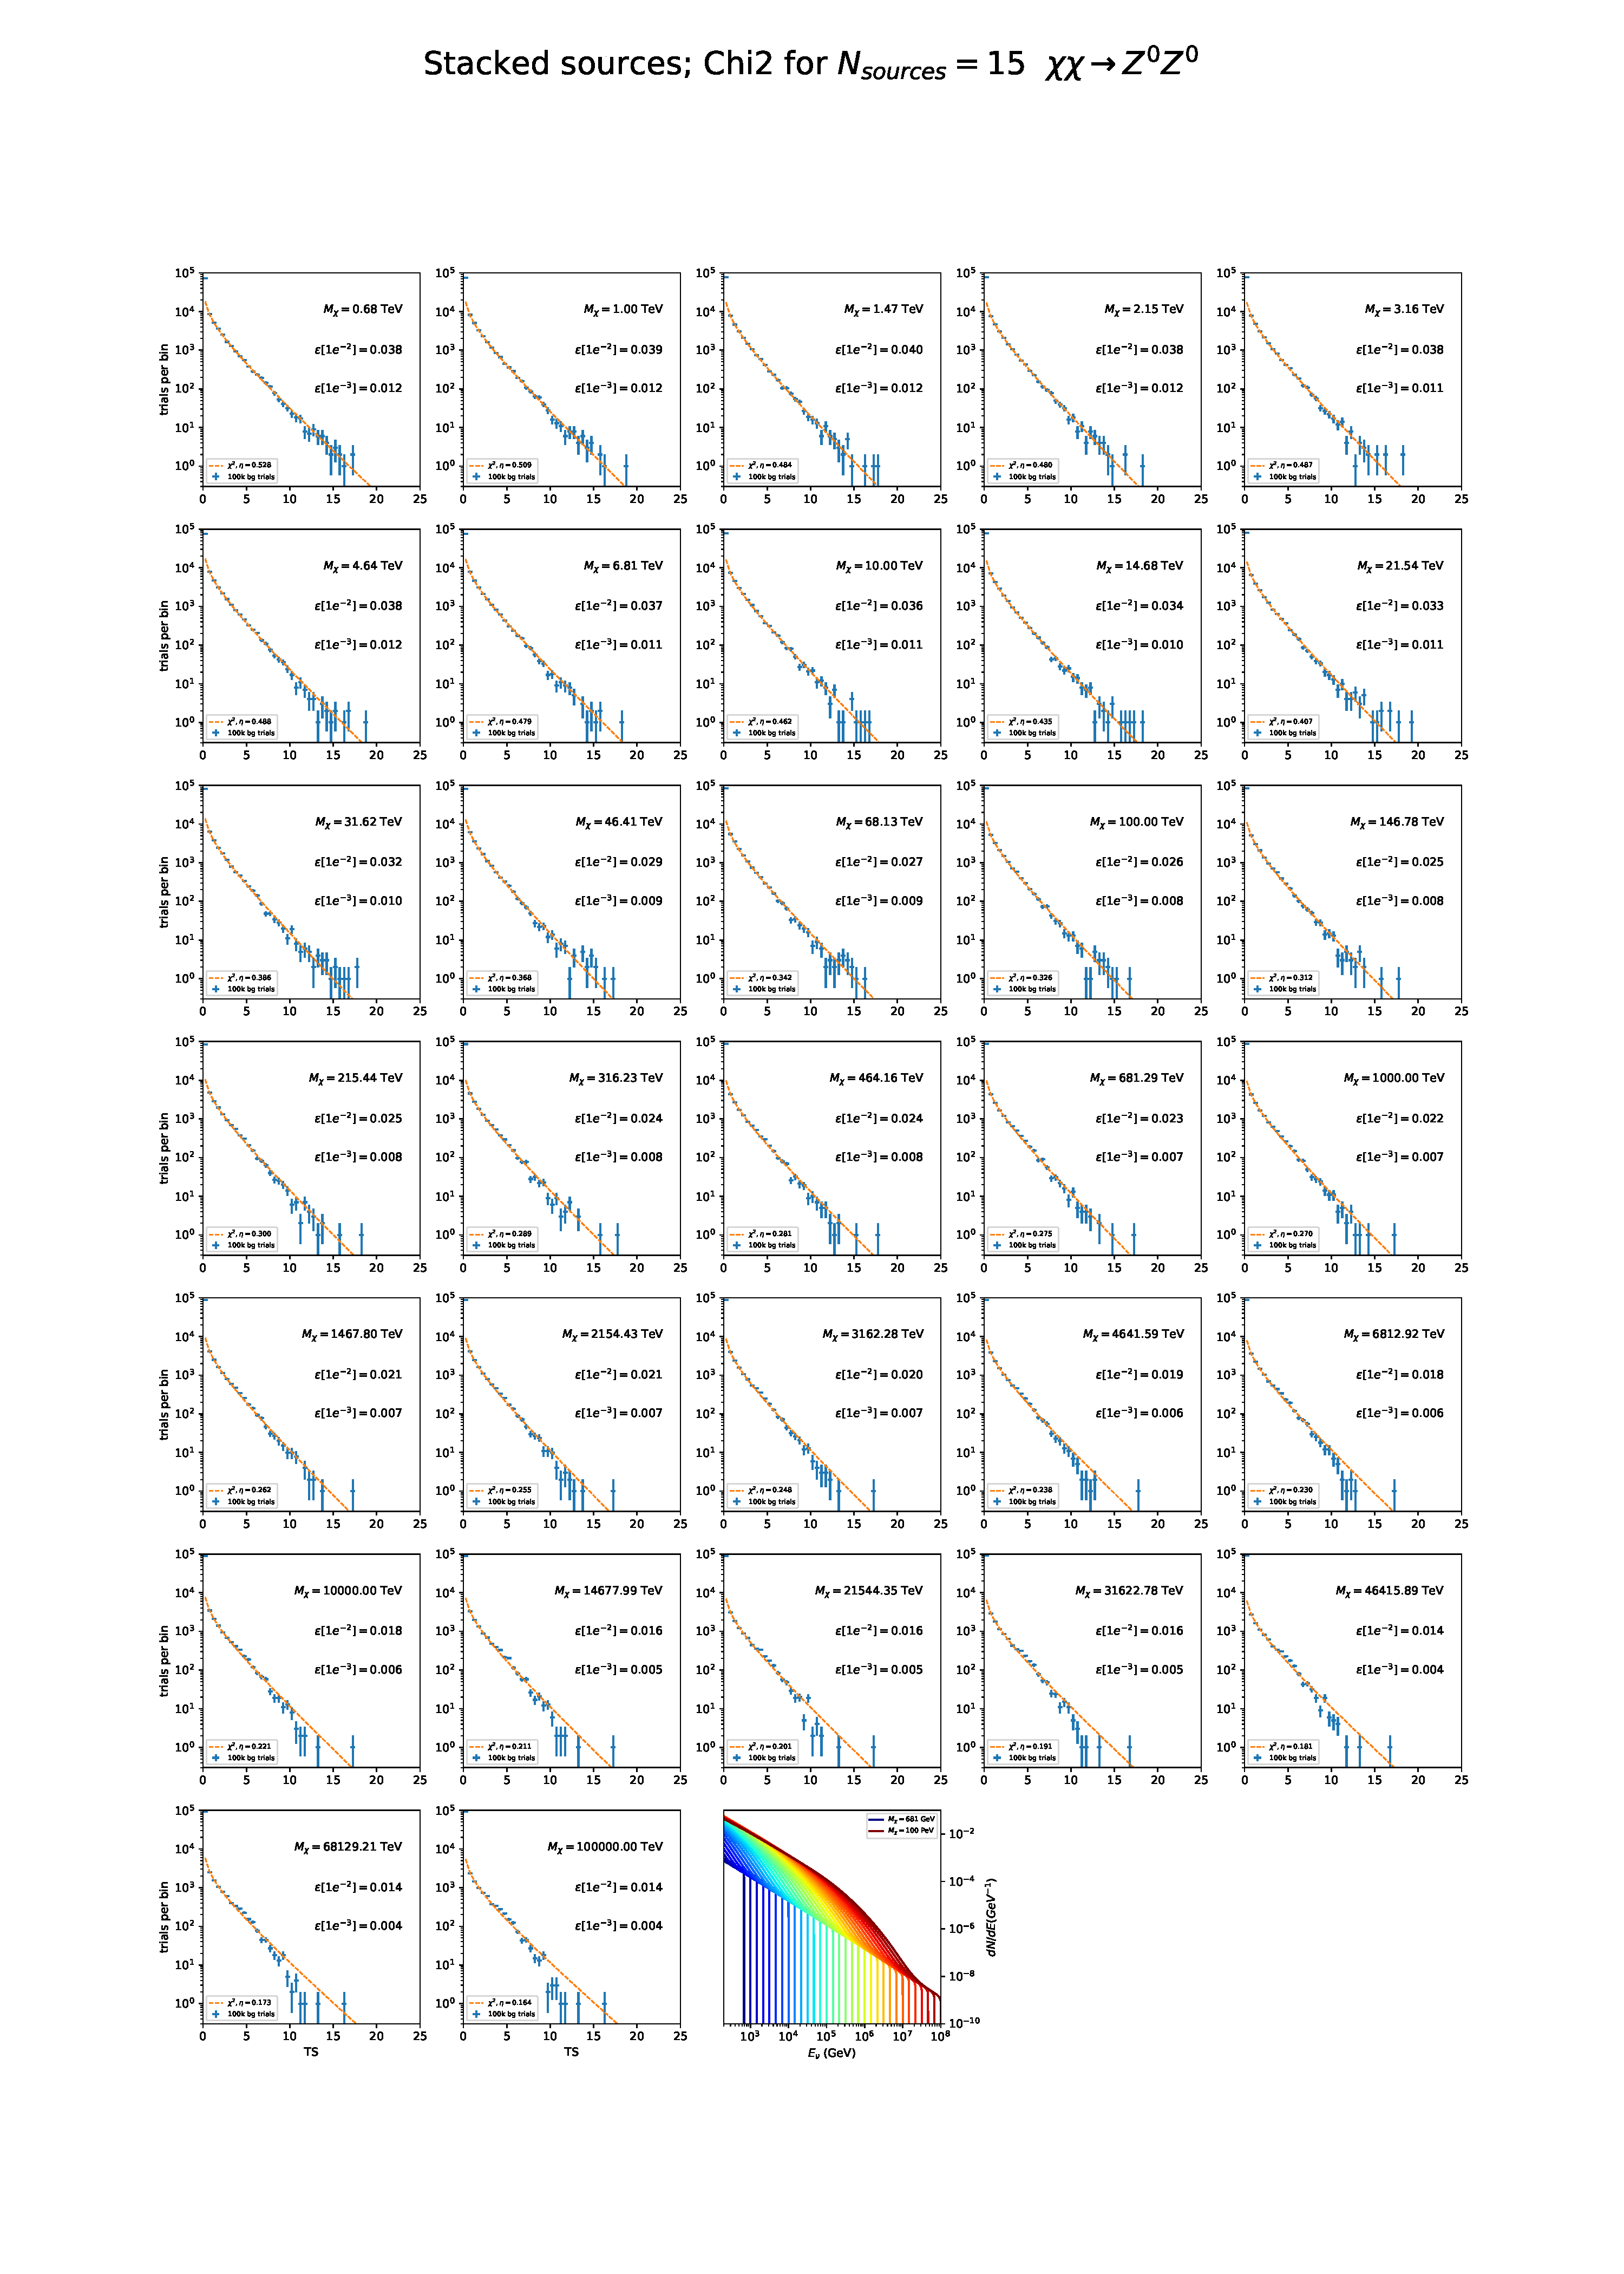
\includegraphics[clip, trim=5cm 6.5cm 4.9cm 8cm, scale=0.345]{figures/ic_DM/dm_plots/stacked_ZZ_chi2_Masspanel_2024-03-23.pdf}
    }\caption{Same as \cref{fig:icDM_Seg1bb_TS} for 15, \GS \J-factor, stacked sources and $\chi\chi \rightarrow$ \pp{Z}.}
    \label{fig:icDM_stact_zz_TS}
\end{figure}

\begin{figure}[ht]
    \centering{
        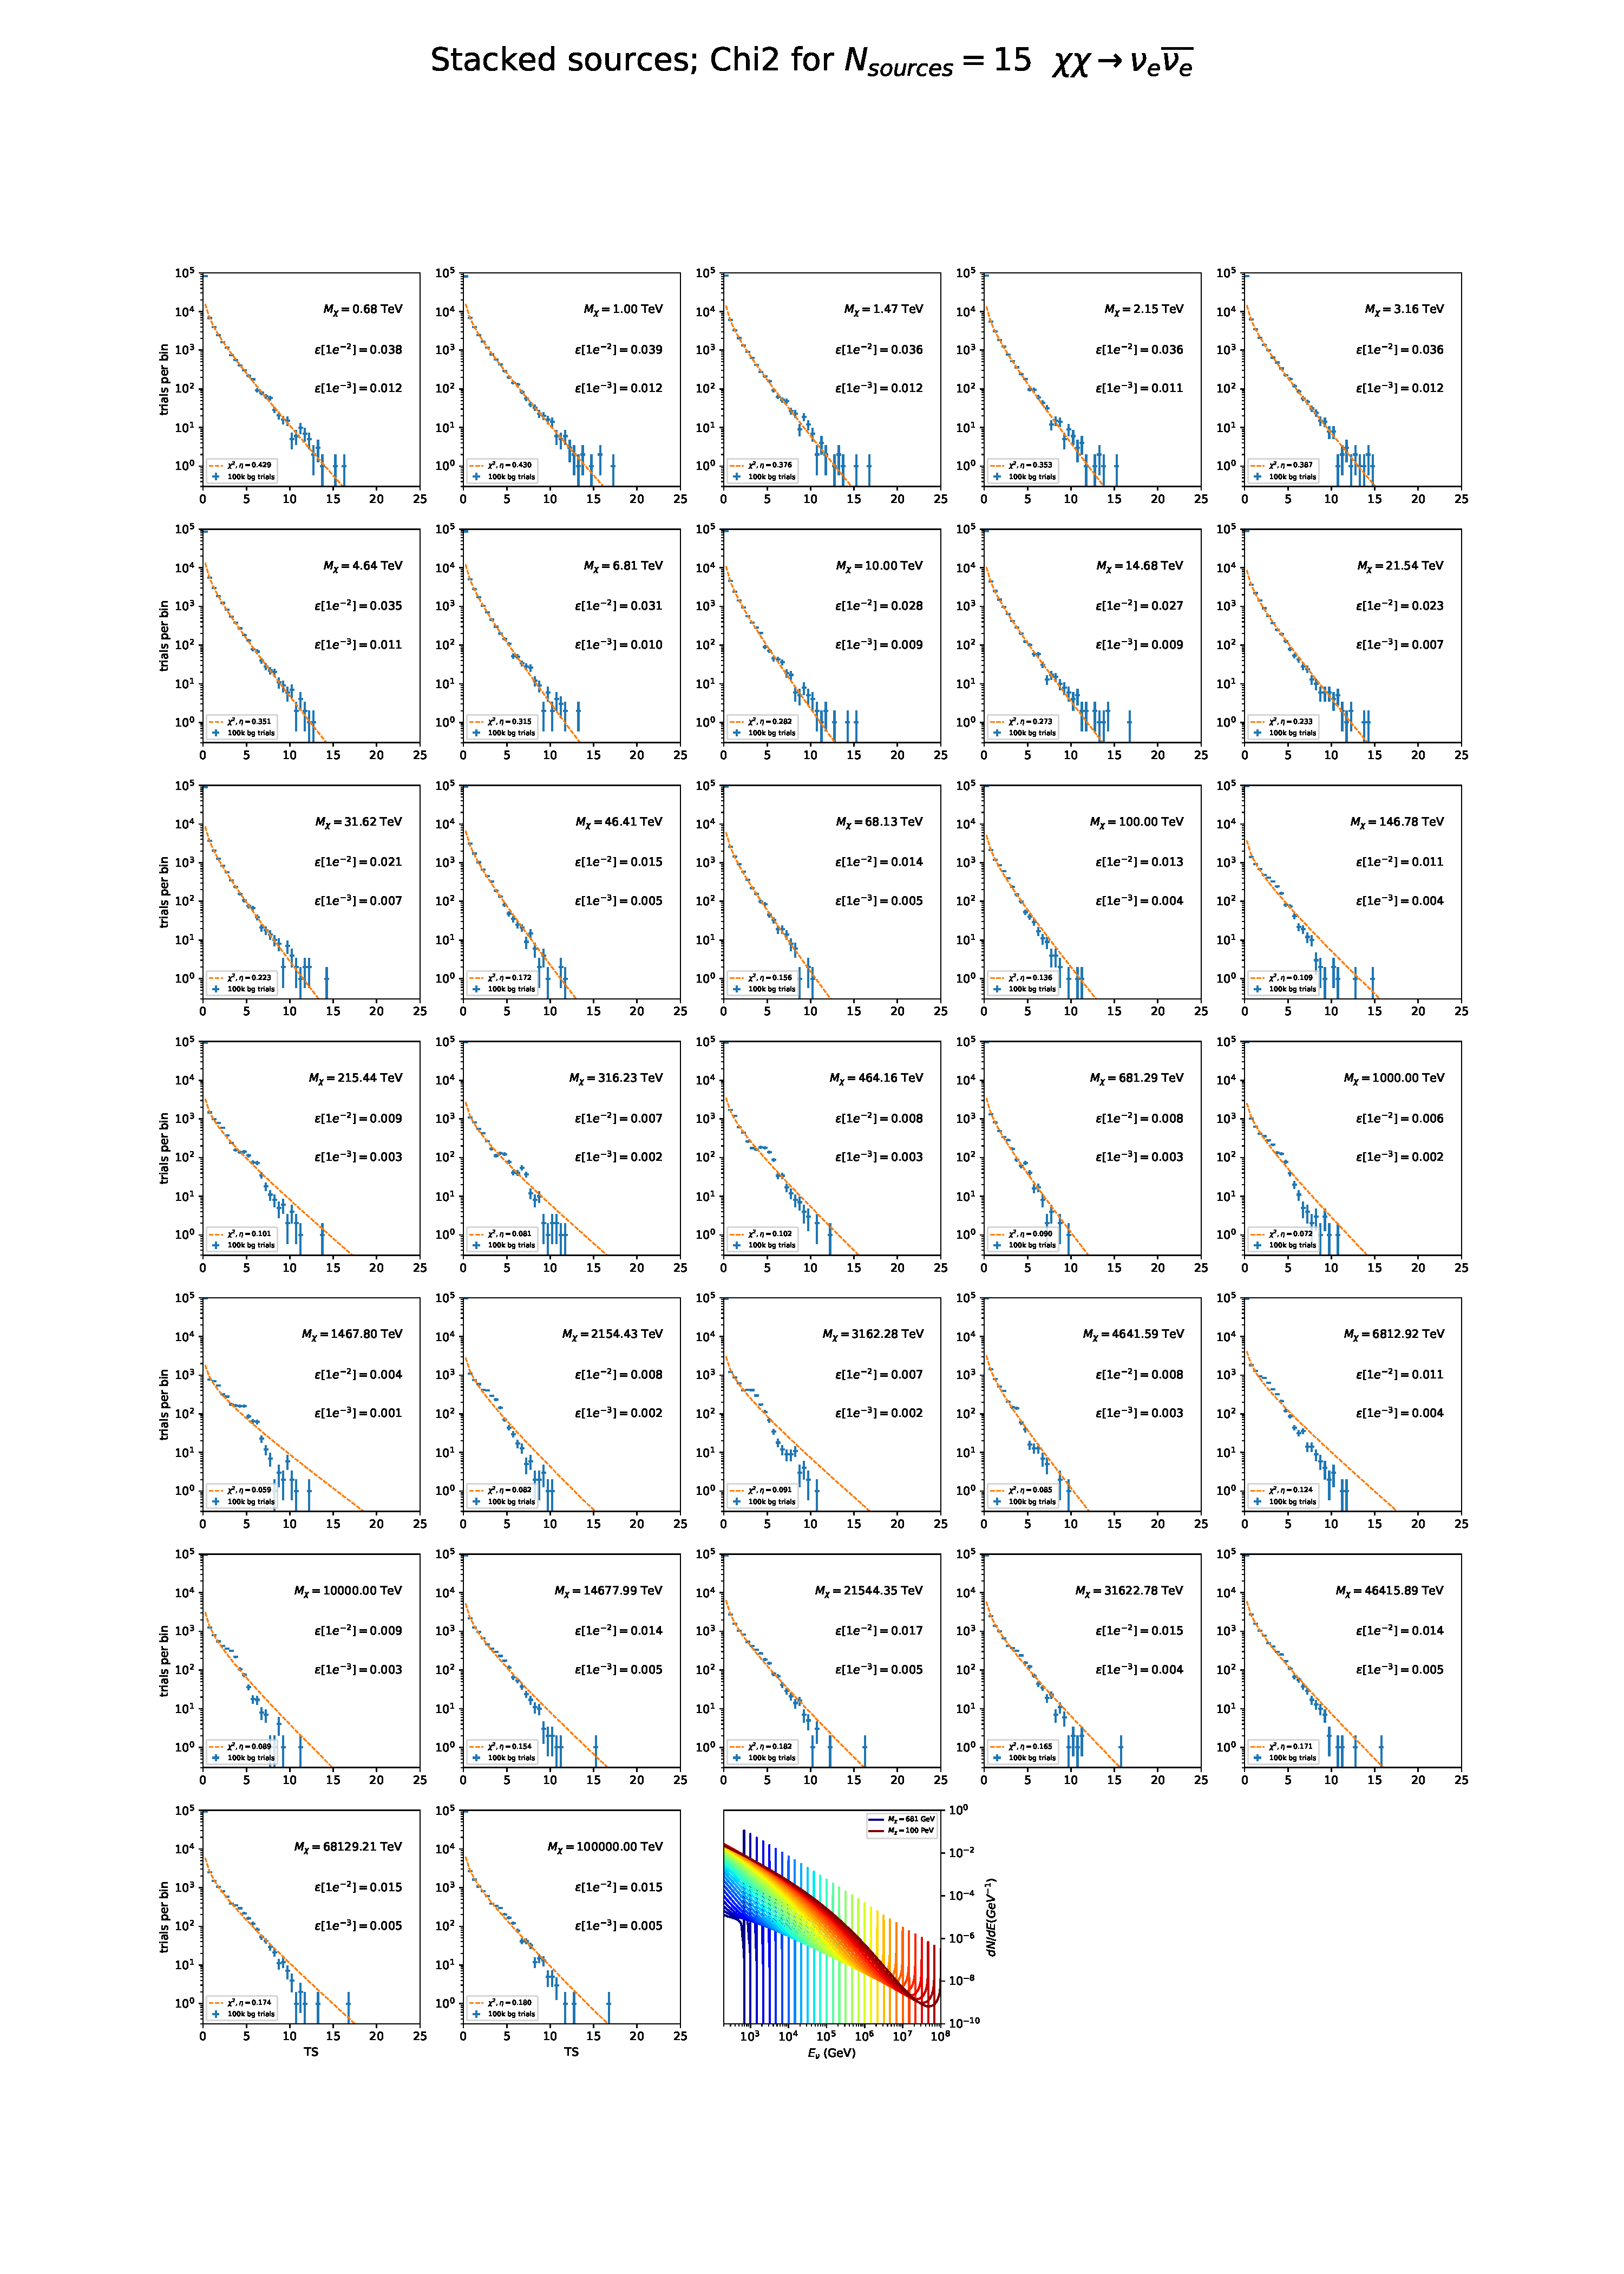
\includegraphics[clip, trim=5cm 6.5cm 4.9cm 8cm, scale=0.345]{figures/ic_DM/dm_plots/stacked_nuenue_chi2_Masspanel_2024-03-23.pdf}
    }\caption{Same as \cref{fig:icDM_Seg1bb_TS} for 15, \GS \J-factor, stacked sources and $\chi\chi \rightarrow$ \parpar{\nu_e}.}
    \label{fig:icDM_stact_nue_TS}
\end{figure}

\begin{figure}[ht]
    \centering{
        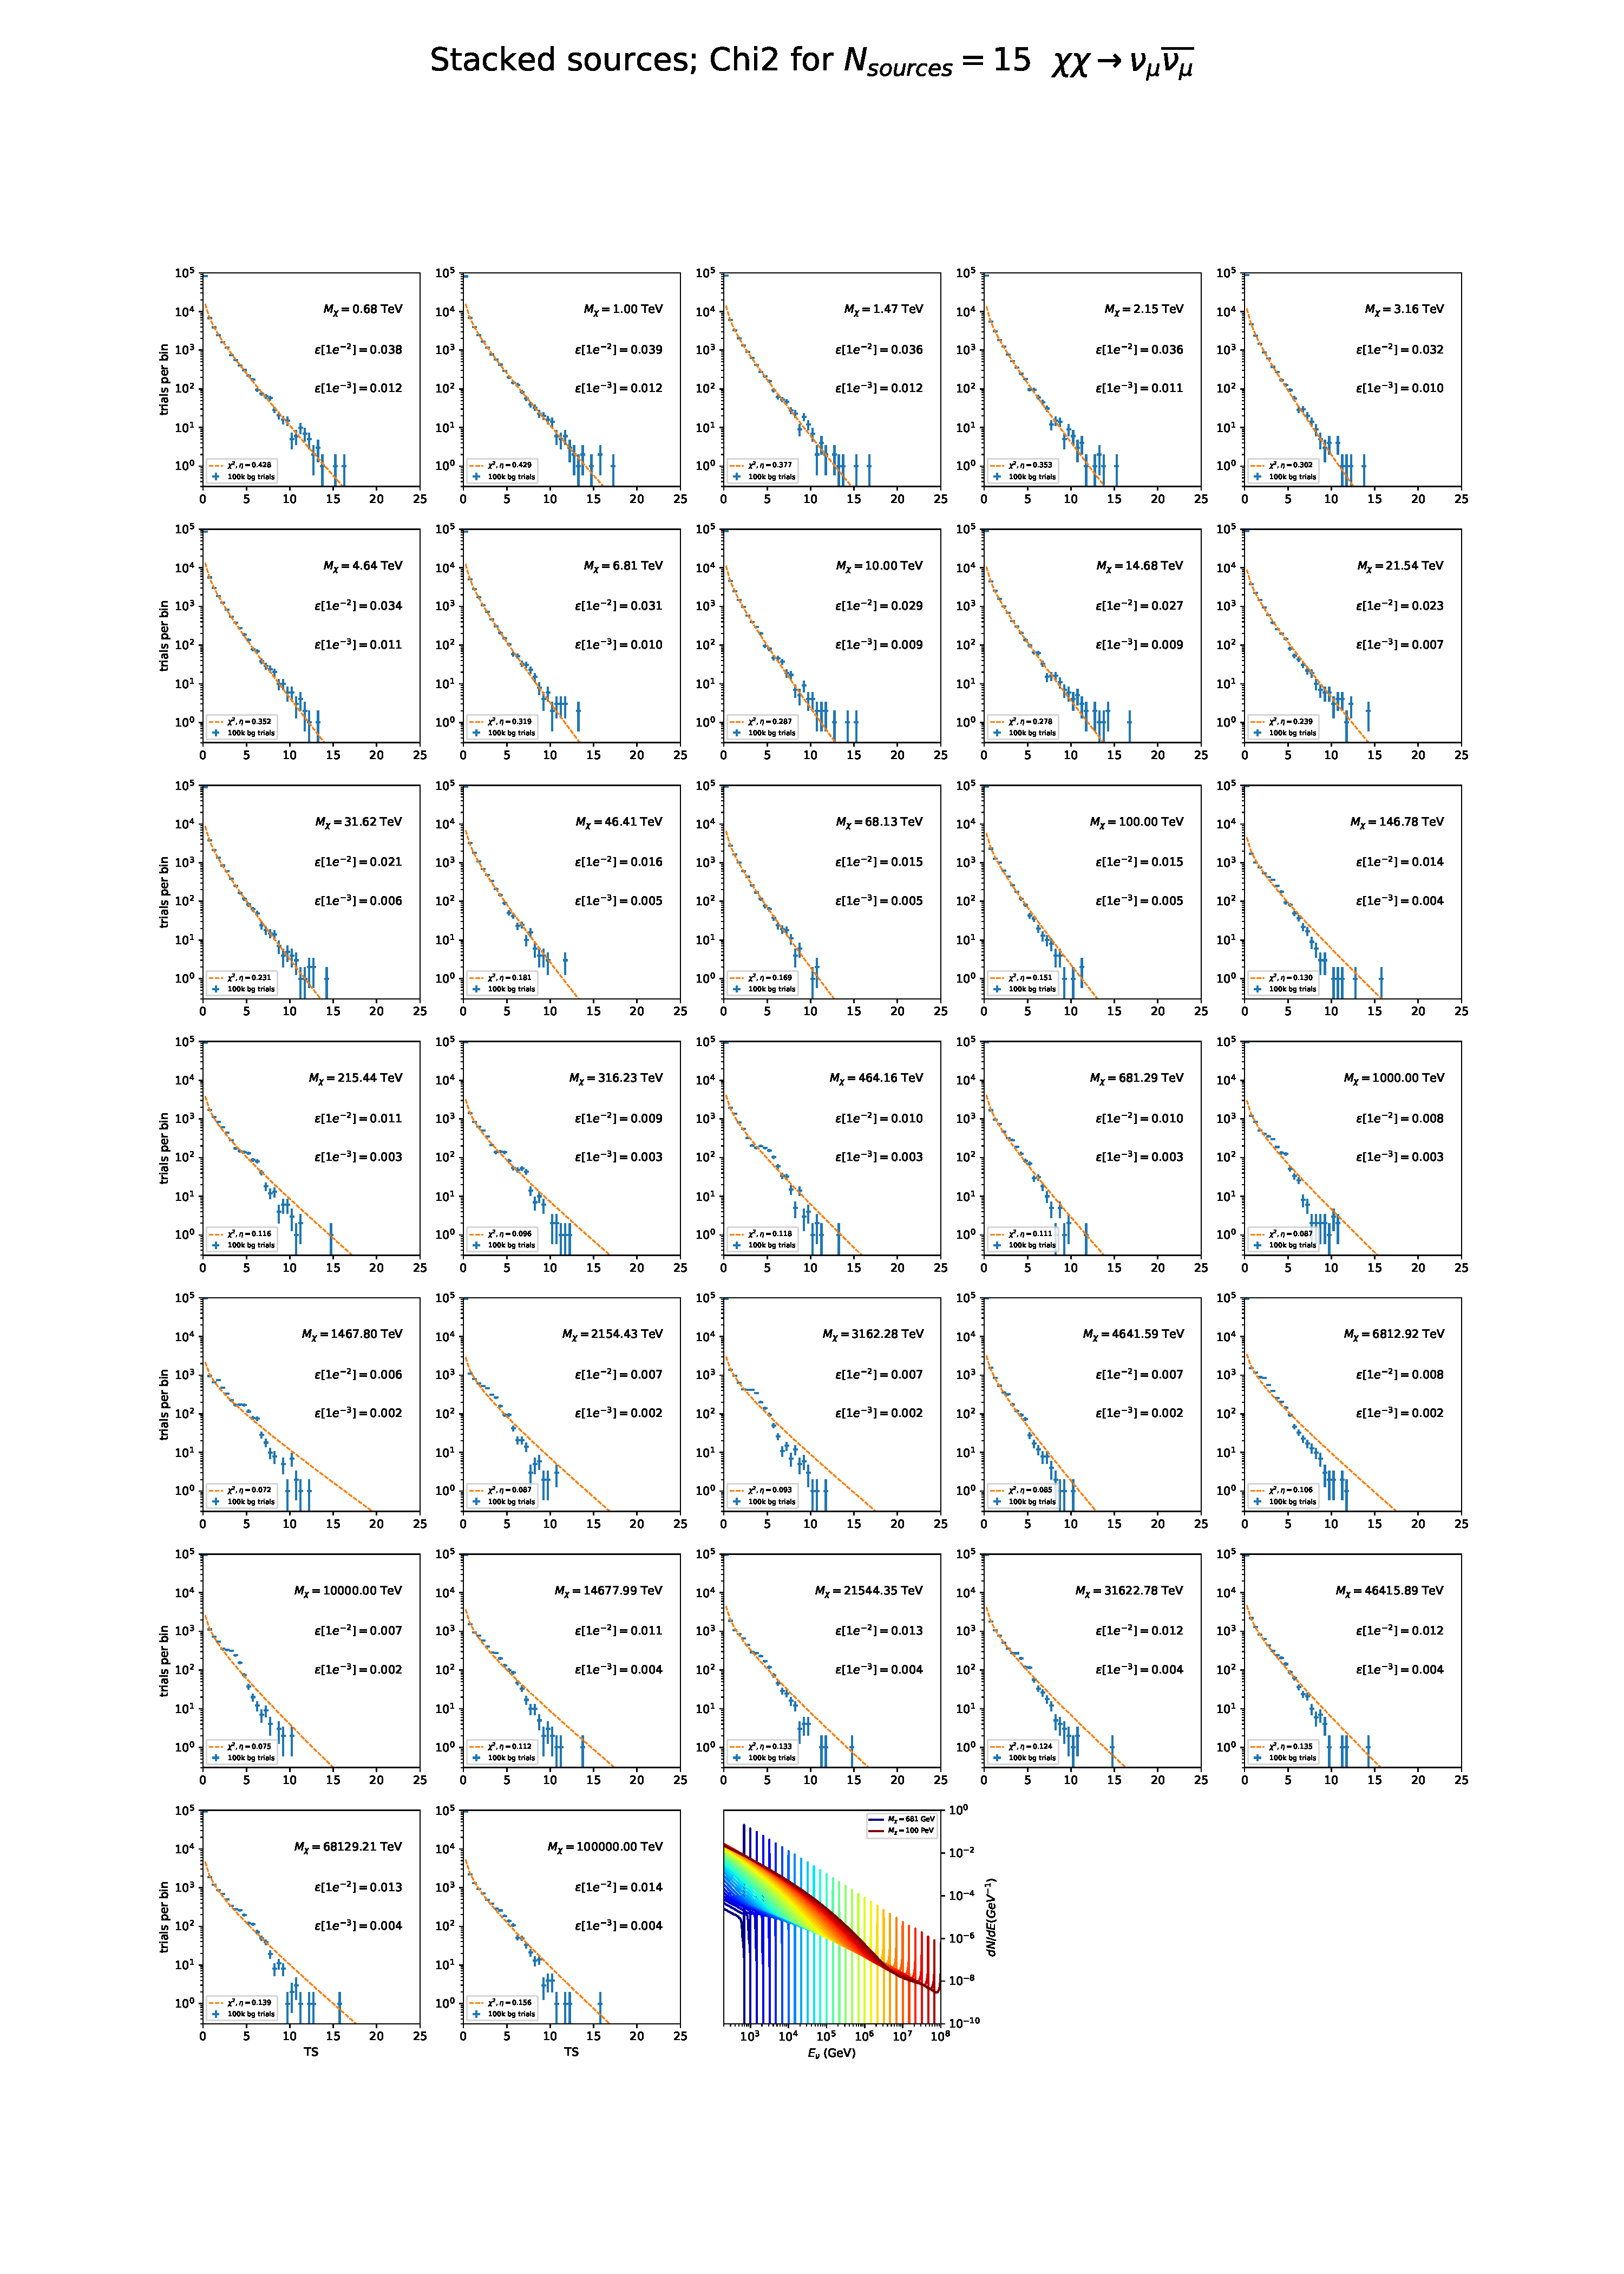
\includegraphics[clip, trim=5cm 6.5cm 4.9cm 8cm, scale=0.345]{figures/ic_DM/dm_plots/stacked_numunumu_chi2_Masspanel_2024-03-23.pdf}
    }\caption{Same as \cref{fig:icDM_Seg1bb_TS} for 15, \GS \J-factor, stacked sources and $\chi\chi \rightarrow$ \parpar{\nu_\mu}.}
    \label{fig:icDM_stact_numu_TS}
\end{figure}

\Cref{fig:icDM_stact_bb_TS} to \Cref{fig:icDM_stact_numu_TS} present the TS distributions for a stacked study of 15 sources with \GS \J-factors on 100,000 trials.
The presentation of these plots are identical to the single source distributions in \cref{sec:icDM_TSperSrc}.

Each subplot, except the final, is the TS distribution for a specific DM mass listed in the subplot.
The final subplot plots the all DM spectral models used as input for the TS distribution calculations with bluer lines indicating lower DM mass and redder indicating higher DM mass.

%%%%%%%%%%%%%%%%%%%%%%%%%%%%%%%%%%%%%%%%%%%%%%%%%%
\section{Signal Recovery} \label{sec:icDM_sig_recovery}
%%%%%%%%%%%%%%%%%%%%%%%%%%%%%%%%%%%%%%%%%%%%%%%%%%

We also wish to understand how well the analysis is able to reconstruct signal neutrinos.
In order to test this, we inject neutrinos from our spectral models randomly then attempt ti discern the number of signal neutrinos in the data.
\Cref{fig:icDM_sigrecovery_1of2} and \Cref{fig:icDM_sigrecovery_2of2} show this study for $\chi\chi \rightarrow$ \parpar{b}, \parpar{t}, and \parpar{\nu_\mu} for a stacked analysis of 15 sources.
We see that the analysis is conservative at smaller $m_\chi$, yet improves at larger $m\chi$.
We also see that the uncertainty around the reconstructed signal events shrinks for the neutrino annihilation spectra.

\begin{figure}[t]
    \centering{
        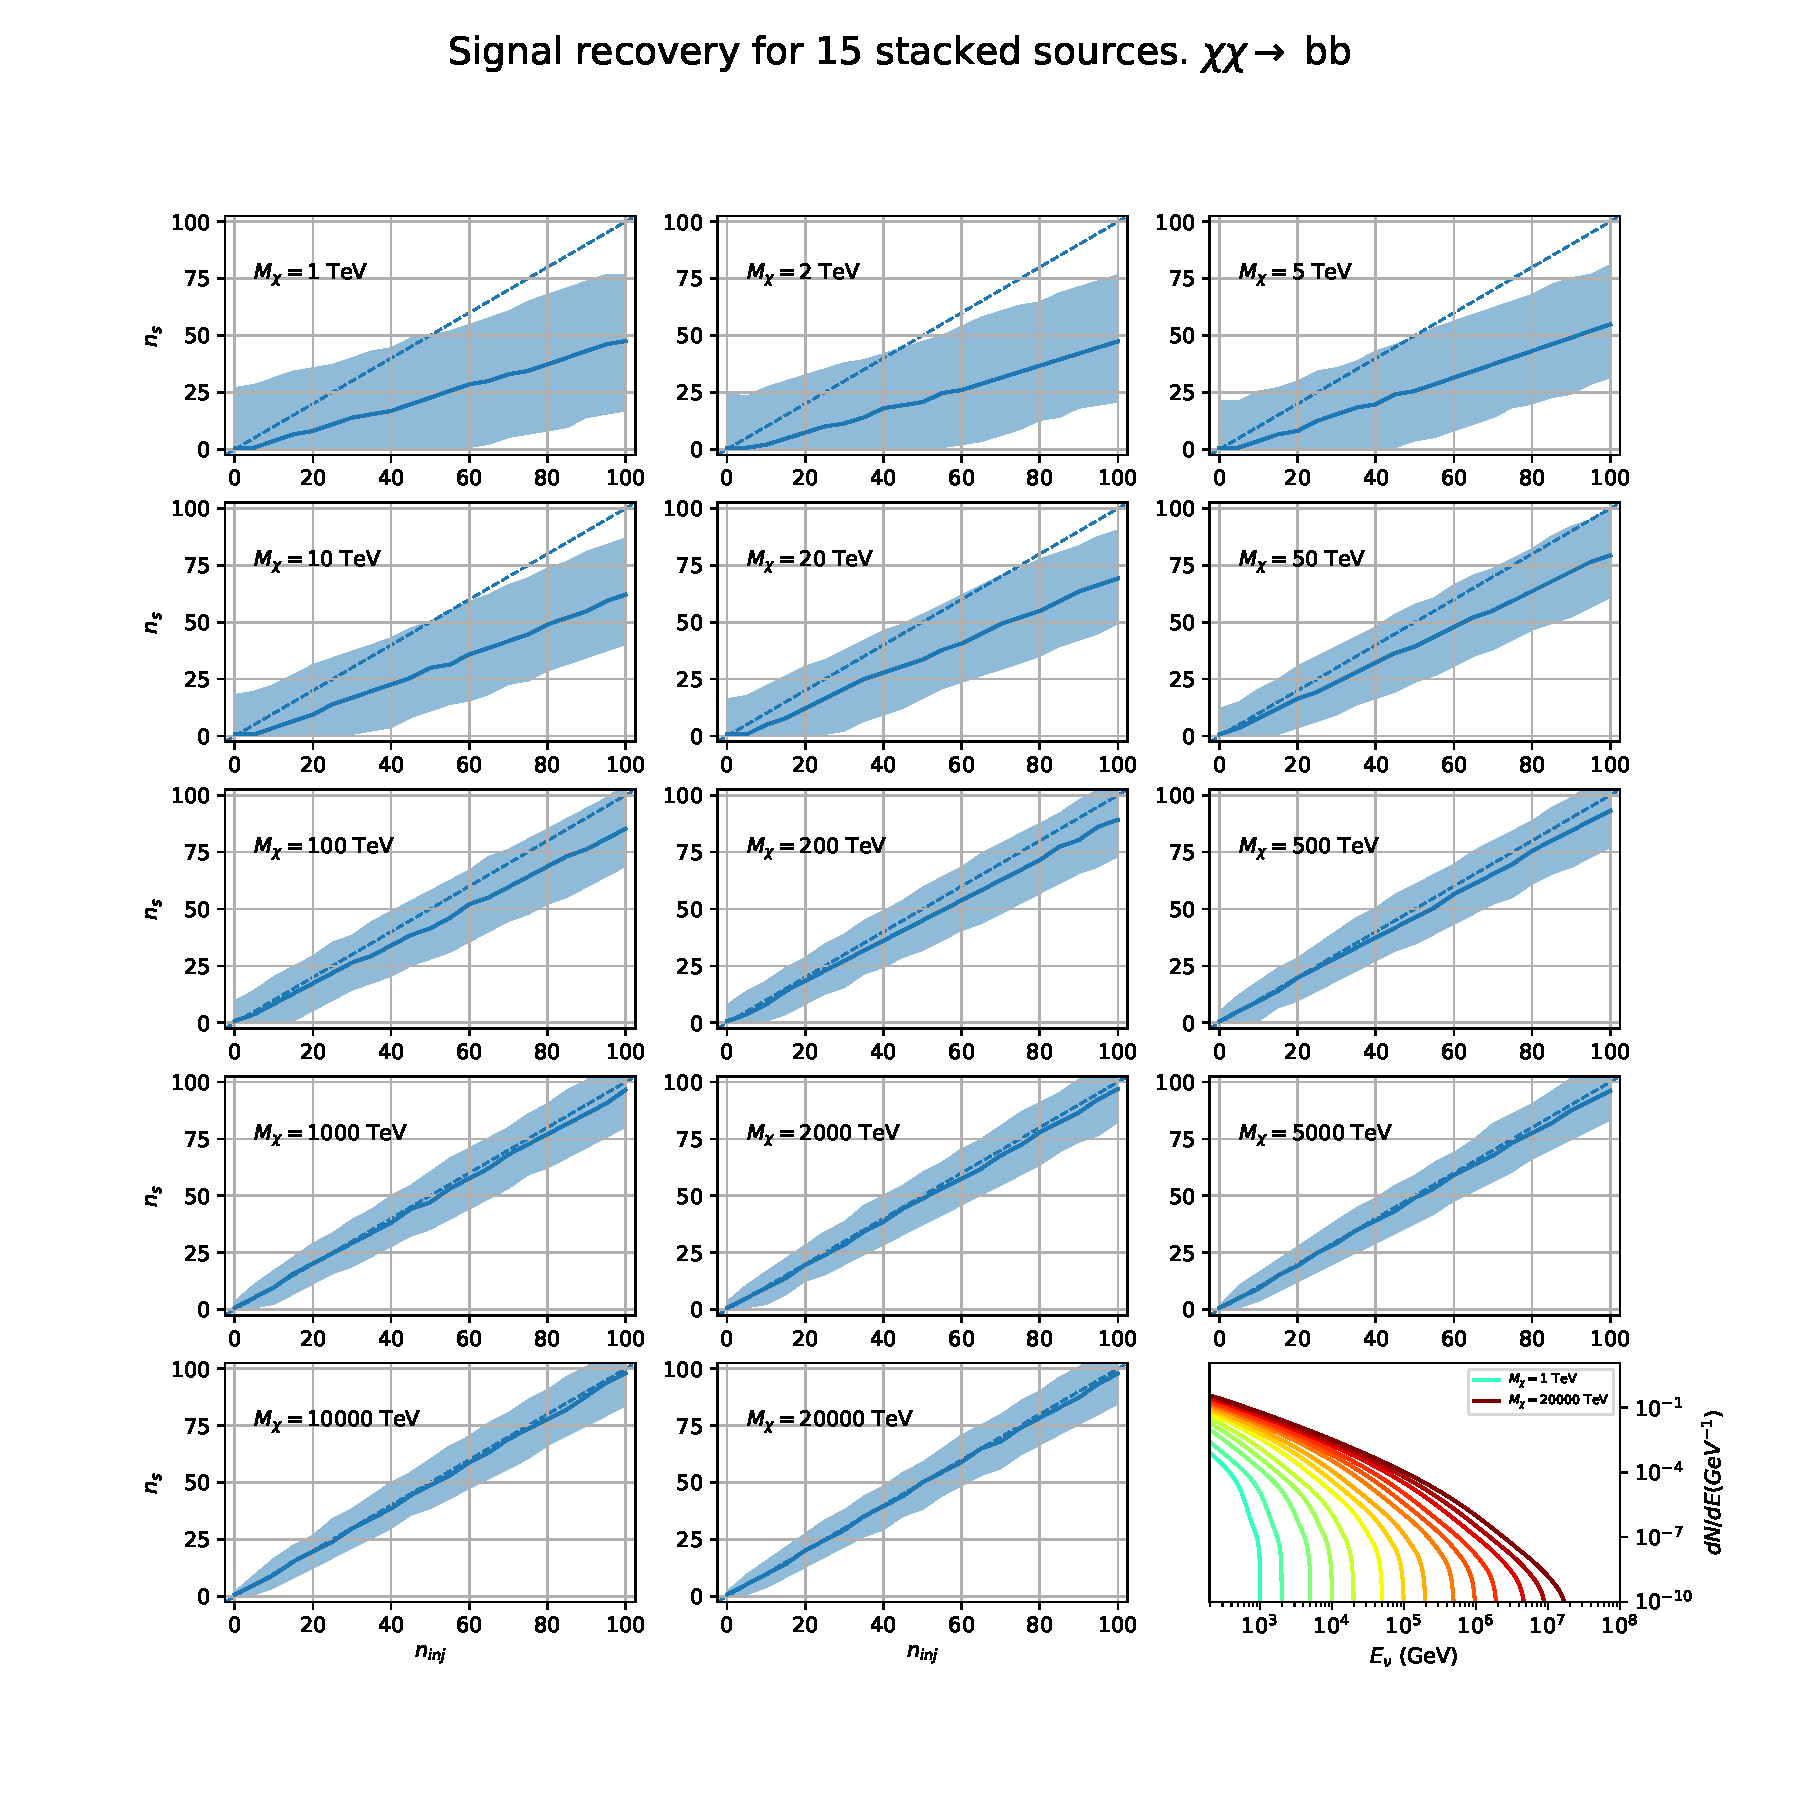
\includegraphics[clip, trim=1.5cm 2.0cm 1.0cm 3.5cm, scale=0.58]{figures/ic_DM/dm_plots/stact_bb_ninj_Masspanel.pdf}
    }\caption{Signal Recovery study for an analysis with 15 stacked sources using the \GS \J-factors \cite{Geringer_Sameth_2015}. Each panel block represents 14 studies for DM mass ranging between 1 TeV and 20 PeV and one annihilation channel. Panel block is for \parpar{t}. Each panel block features every spectral model used as input in the bottom-right subpanel. The remaining panels show $n_\mathrm{inj}$ as the number of signal events injected into background simulation. Whereas, $n_s$ is the number of signal events recovered from analyzing the injected simulation. Blue line represents the median values of 100 simulations. Light blue bands show the $1\sigma$ statistical uncertainty around the median.}
    \label{fig:icDM_sigrecovery_1of2}
\end{figure}

\begin{figure}[t]
    \centering{
        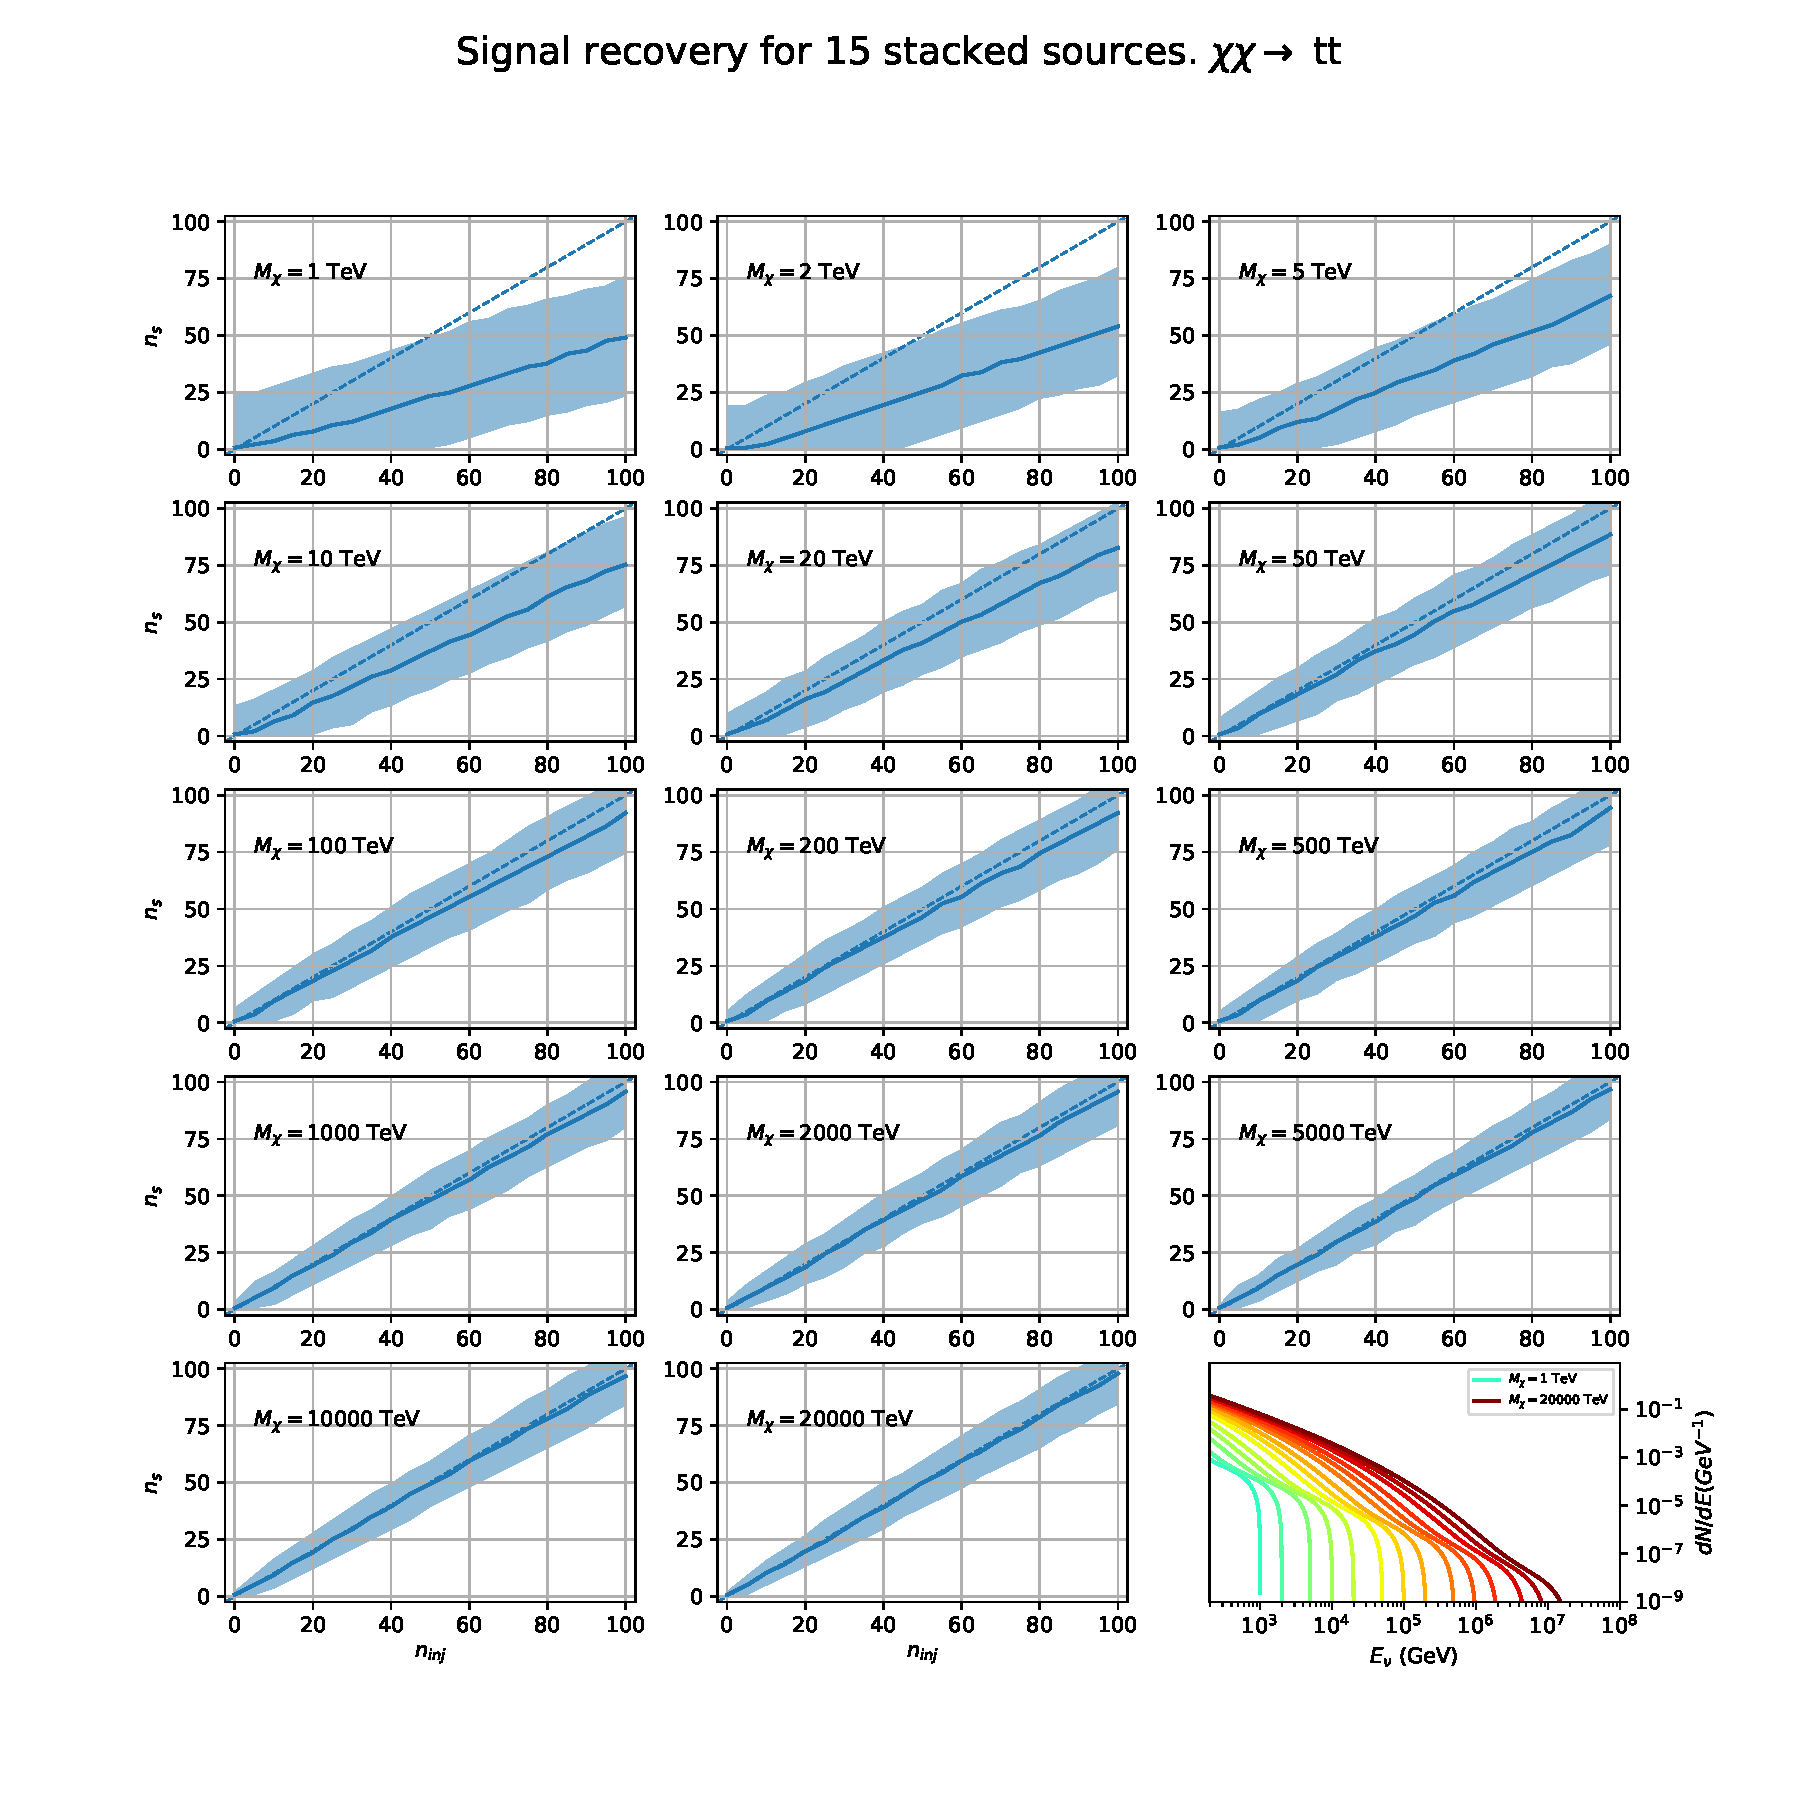
\includegraphics[clip, trim=1.5cm 2.0cm 1.0cm 3.5cm, scale=0.42]{figures/ic_DM/dm_plots/stact_tt_ninj_Masspanel.pdf}
        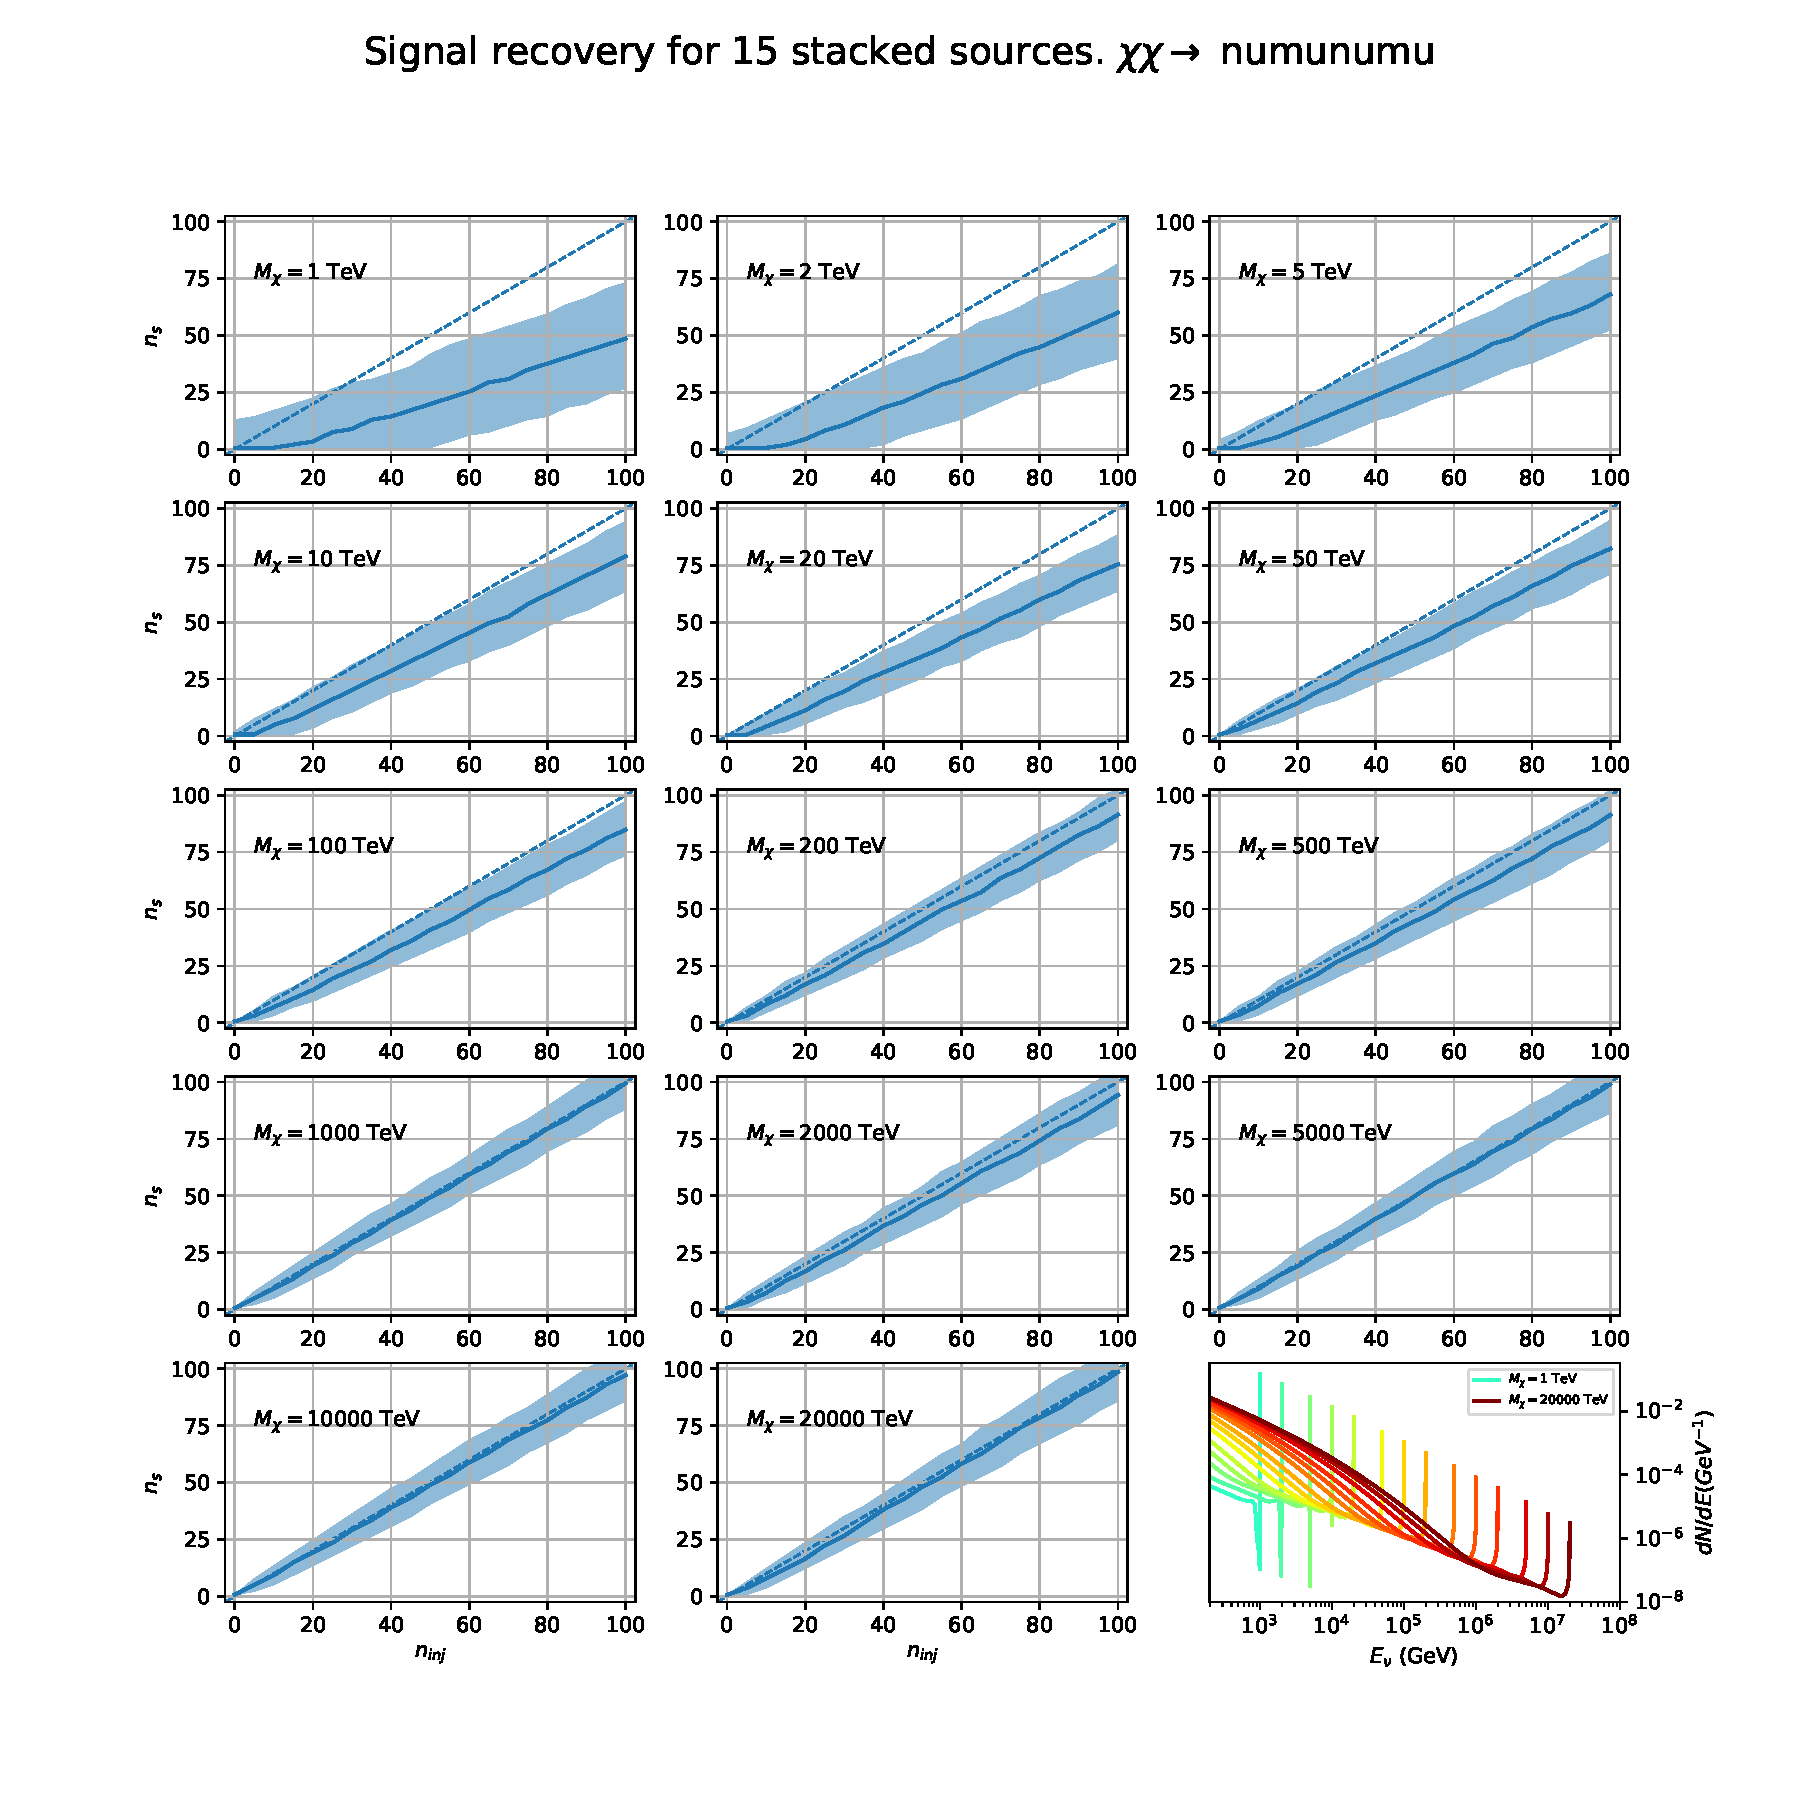
\includegraphics[clip, trim=1.5cm 2.0cm 1.0cm 3.5cm, scale=0.42]{figures/ic_DM/dm_plots/stact_numunumu_ninj_Masspanel.pdf}
    }\caption{Same as \cref{fig:icDM_sigrecovery_1of2} but for $\chi\chi \rightarrow$ \parpar{b} (top) and \parpar{\nu_\mu} (bottom).}
    \label{fig:icDM_sigrecovery_2of2}
\end{figure}

%%%%%%%%%%%%%%%%%%%%%%%%%%%%%%%%%%%%%%%%%%%%%%%%%%
\subsection{Sensitivities} \label{sec:icDM_sensitivity}
%%%%%%%%%%%%%%%%%%%%%%%%%%%%%%%%%%%%%%%%%%%%%%%%%%

In IceCube, we usually define the 90\% confidence level (CL), as the minimum number of signal events ($n_s$) required to have a Type I error rate smaller than 0.5 and Type II error rate of 0.1.
We compute  $n_s$ from the following equation
\svFromNSig
to extract the sensitivity on the dark matter annihilation cross-section.
$T_\mathrm{live} $ is the detector livetime, $ A_\mathrm{eff} $ is the effective area of the detector, and $ E_\mathrm{min} $, $ E_\mathrm{max} $ are the minimum, maximum energies of the expected neutrinos, respectively.

Sensitivities are calculated for each source individually as if they were the only source and as a stack over 1000 trials.
From \cref{eq:sv_from_nsig} and \cref{eq:id_dm_flux} we can compute the \sv~at a 90\% confidence level.
\Cref{fig:icDM_sensitivity_1of2} and \cref{fig:icDM_sensitivity_2of2} show the sensitivities for some DM annihilation channels.
Not all channels computed successfully in time for the writing of this dissertation.
Among channels missing include two neutrino flavors: $e$ and $\tau$.

\begin{figure}[t]
    \centering{
        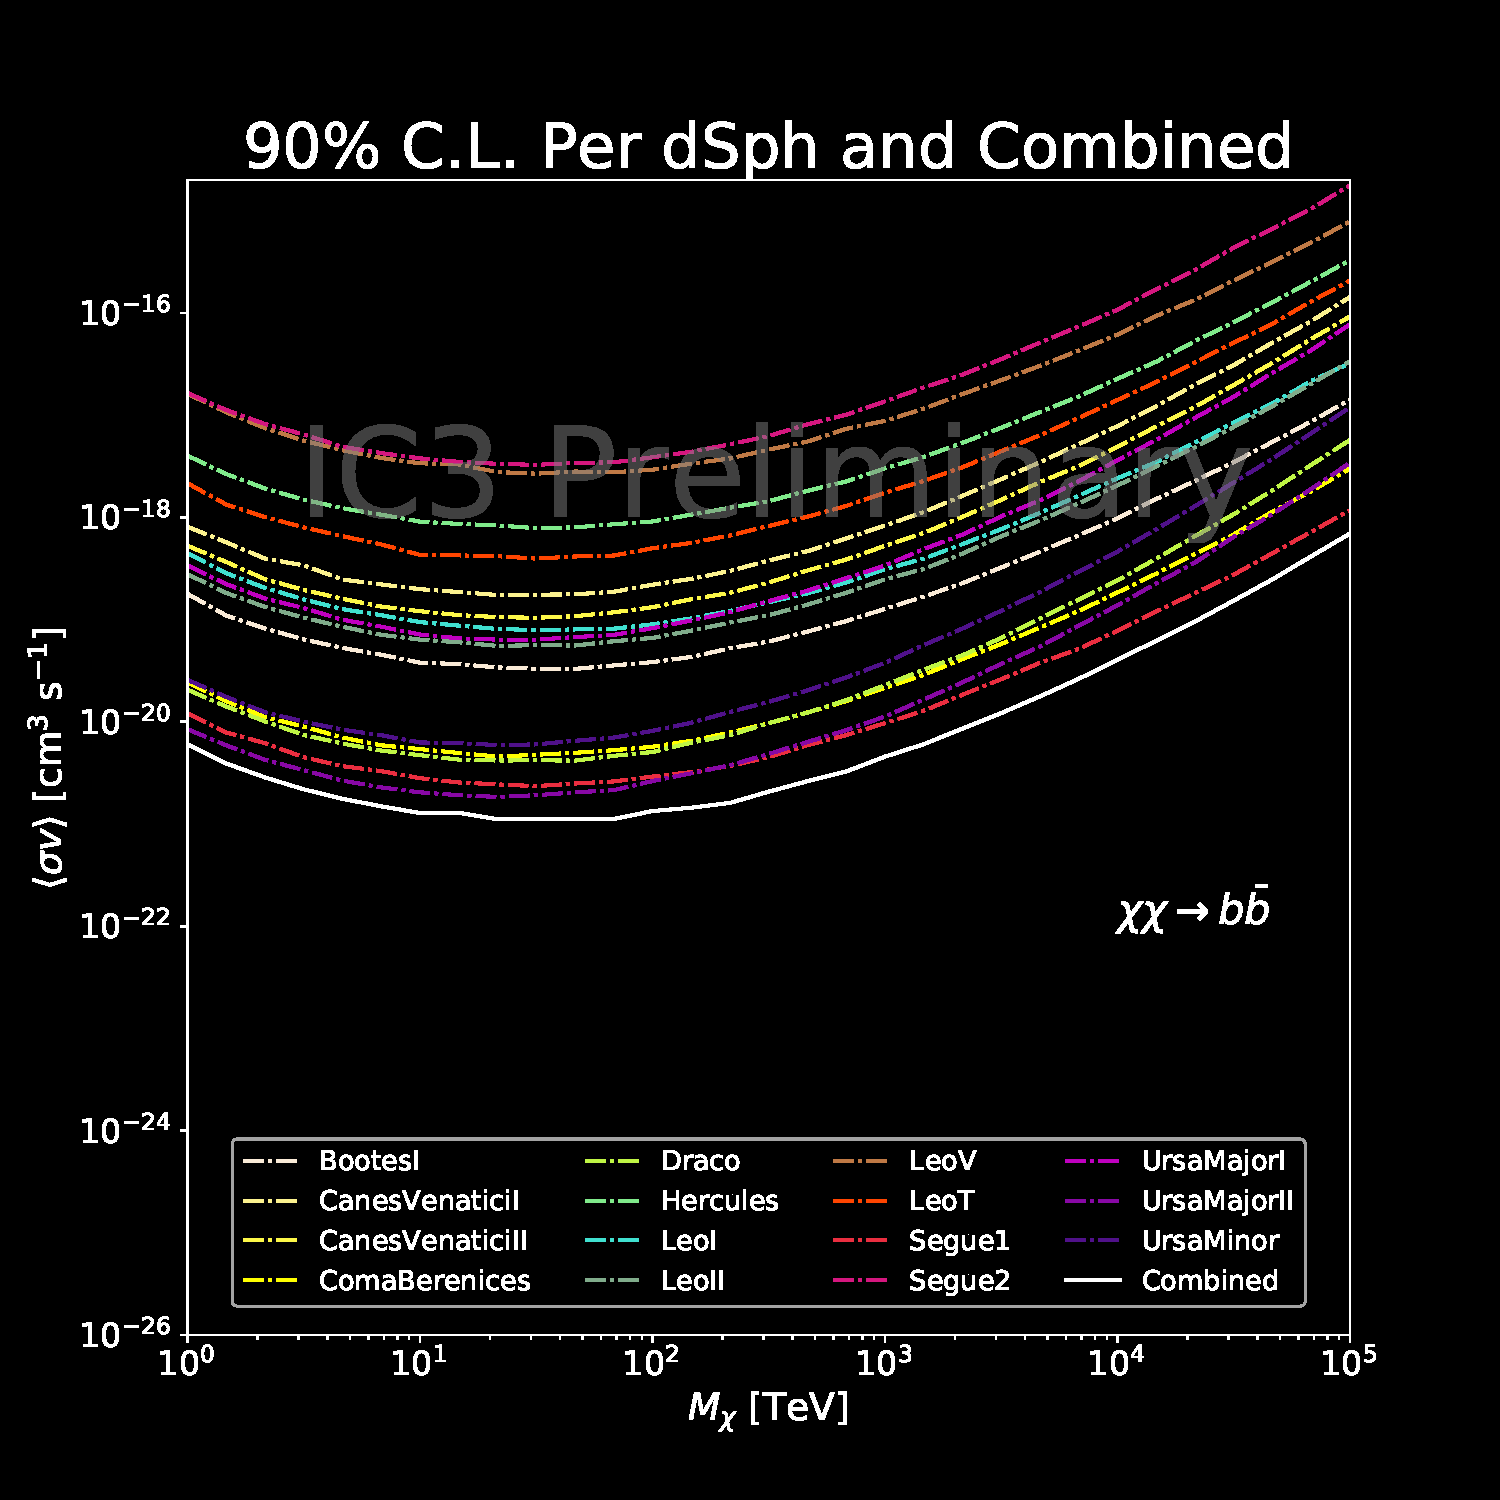
\includegraphics[scale=0.275]{figures/ic_DM/dm_plots/bb_money_plot_comb.pdf}
        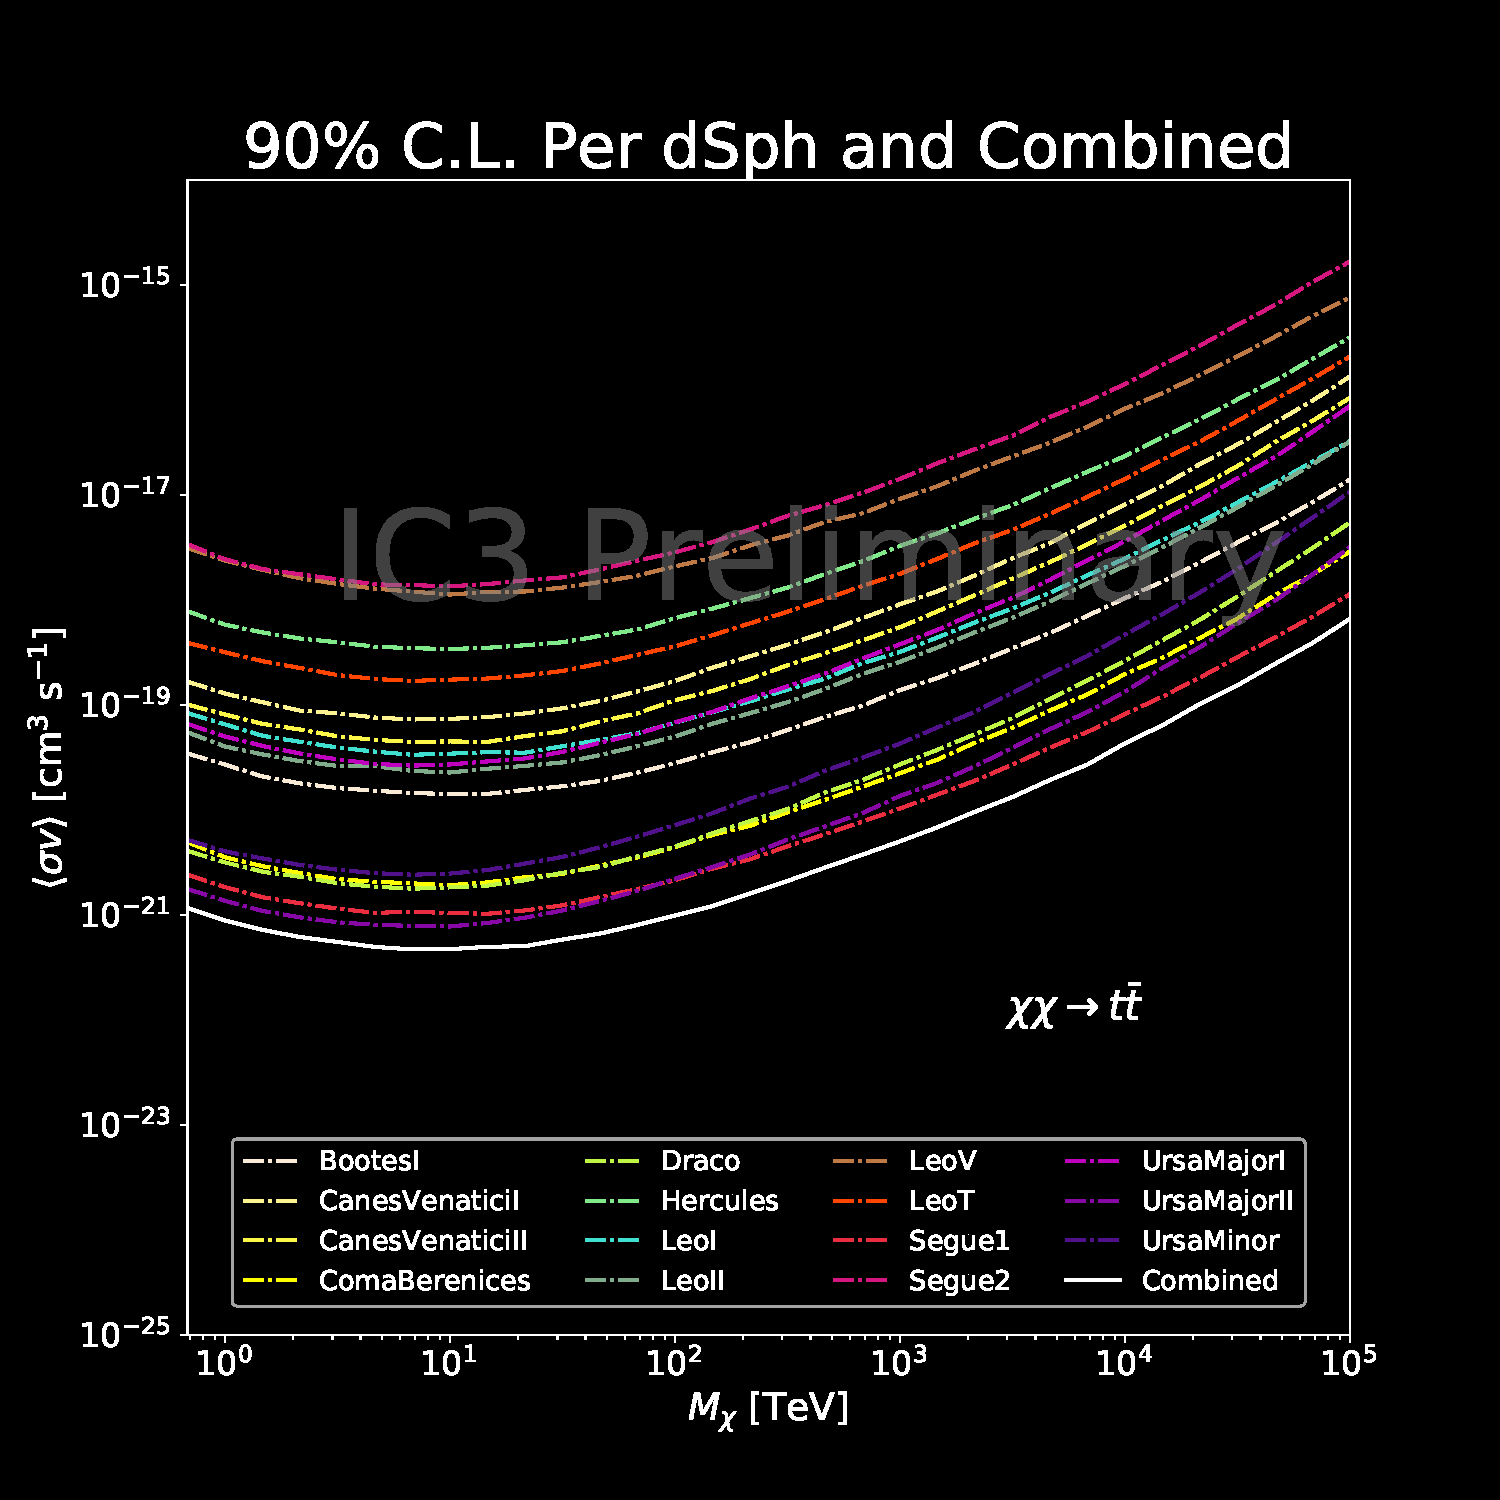
\includegraphics[scale=0.275]{figures/ic_DM/dm_plots/tt_money_plot_comb.pdf}
        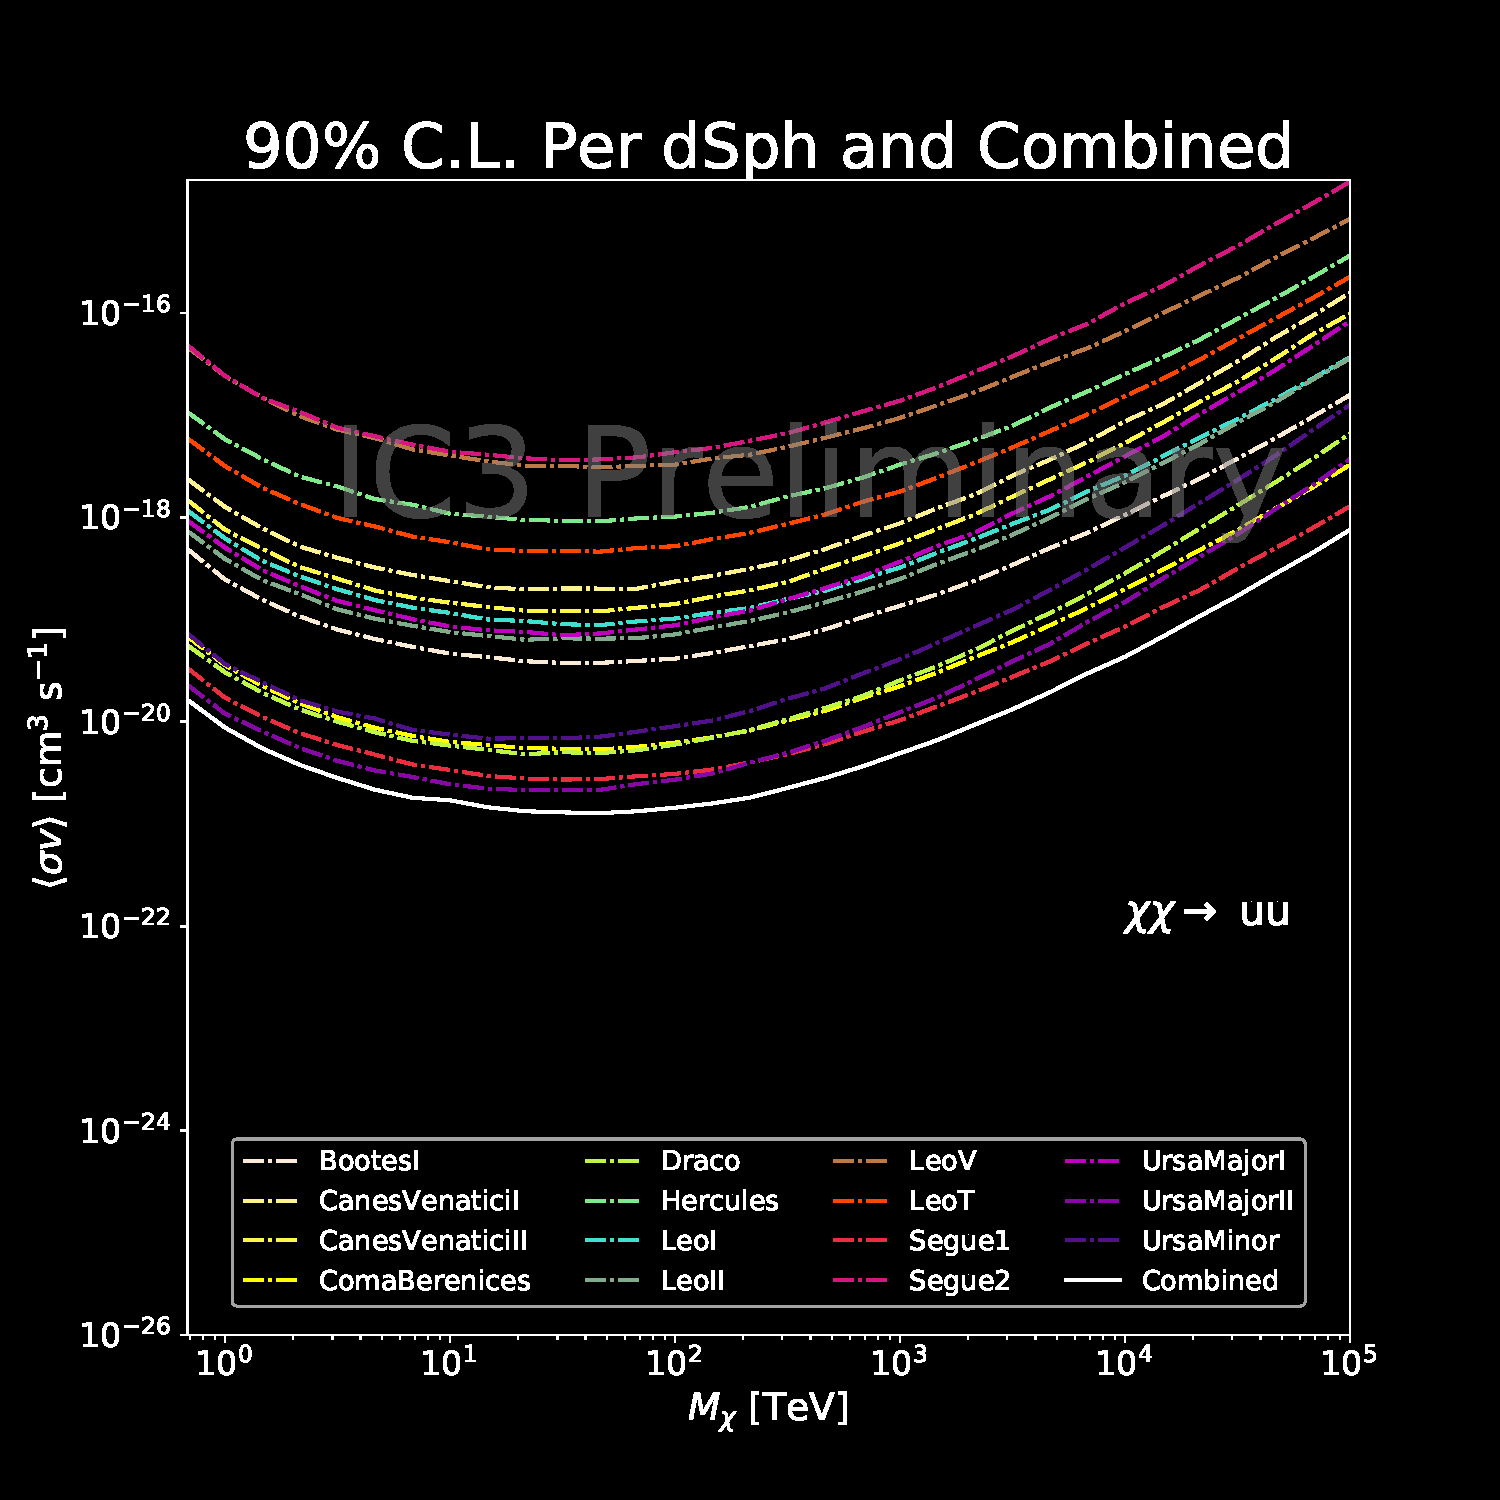
\includegraphics[scale=0.275]{figures/ic_DM/dm_plots/uu_money_plot_comb.pdf}
        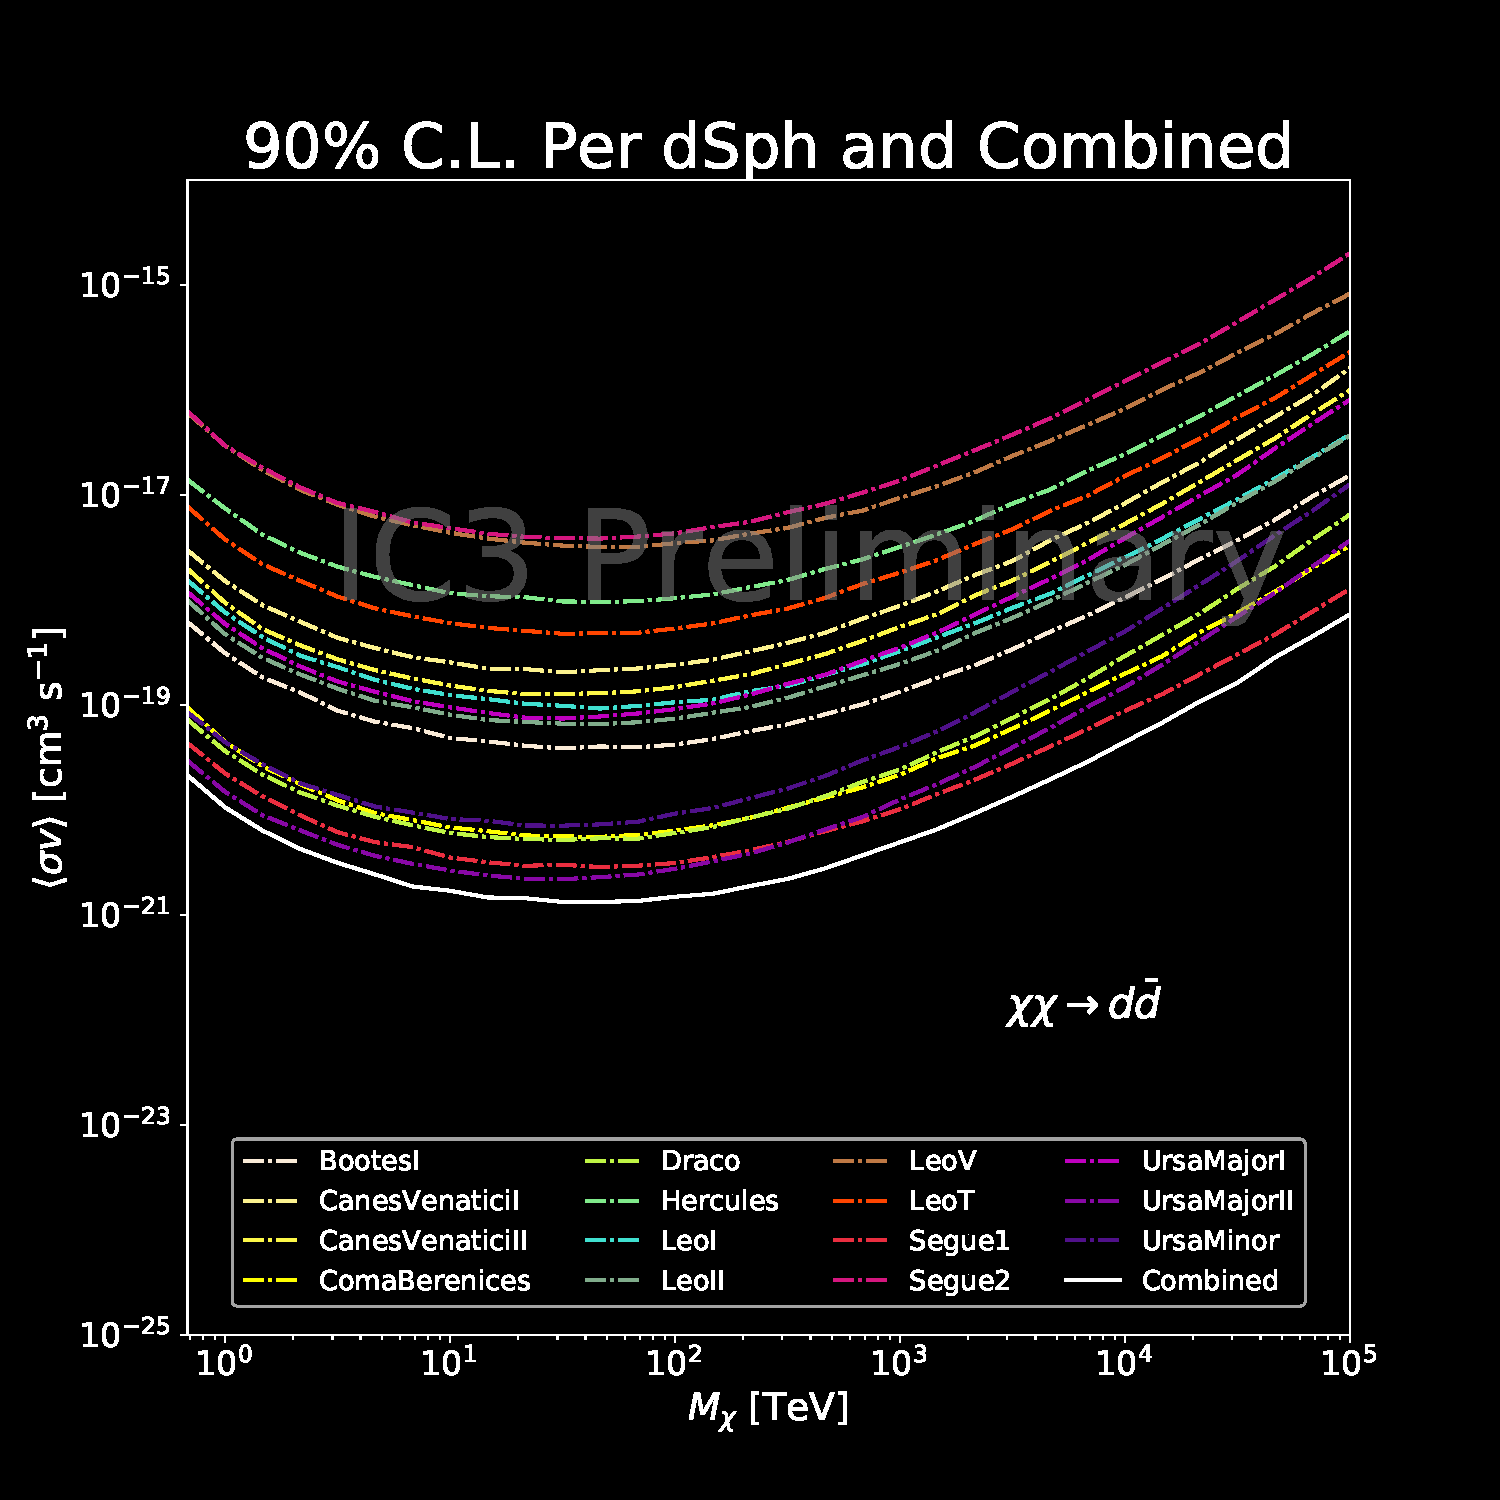
\includegraphics[scale=0.275]{figures/ic_DM/dm_plots/dd_money_plot_comb.pdf}
        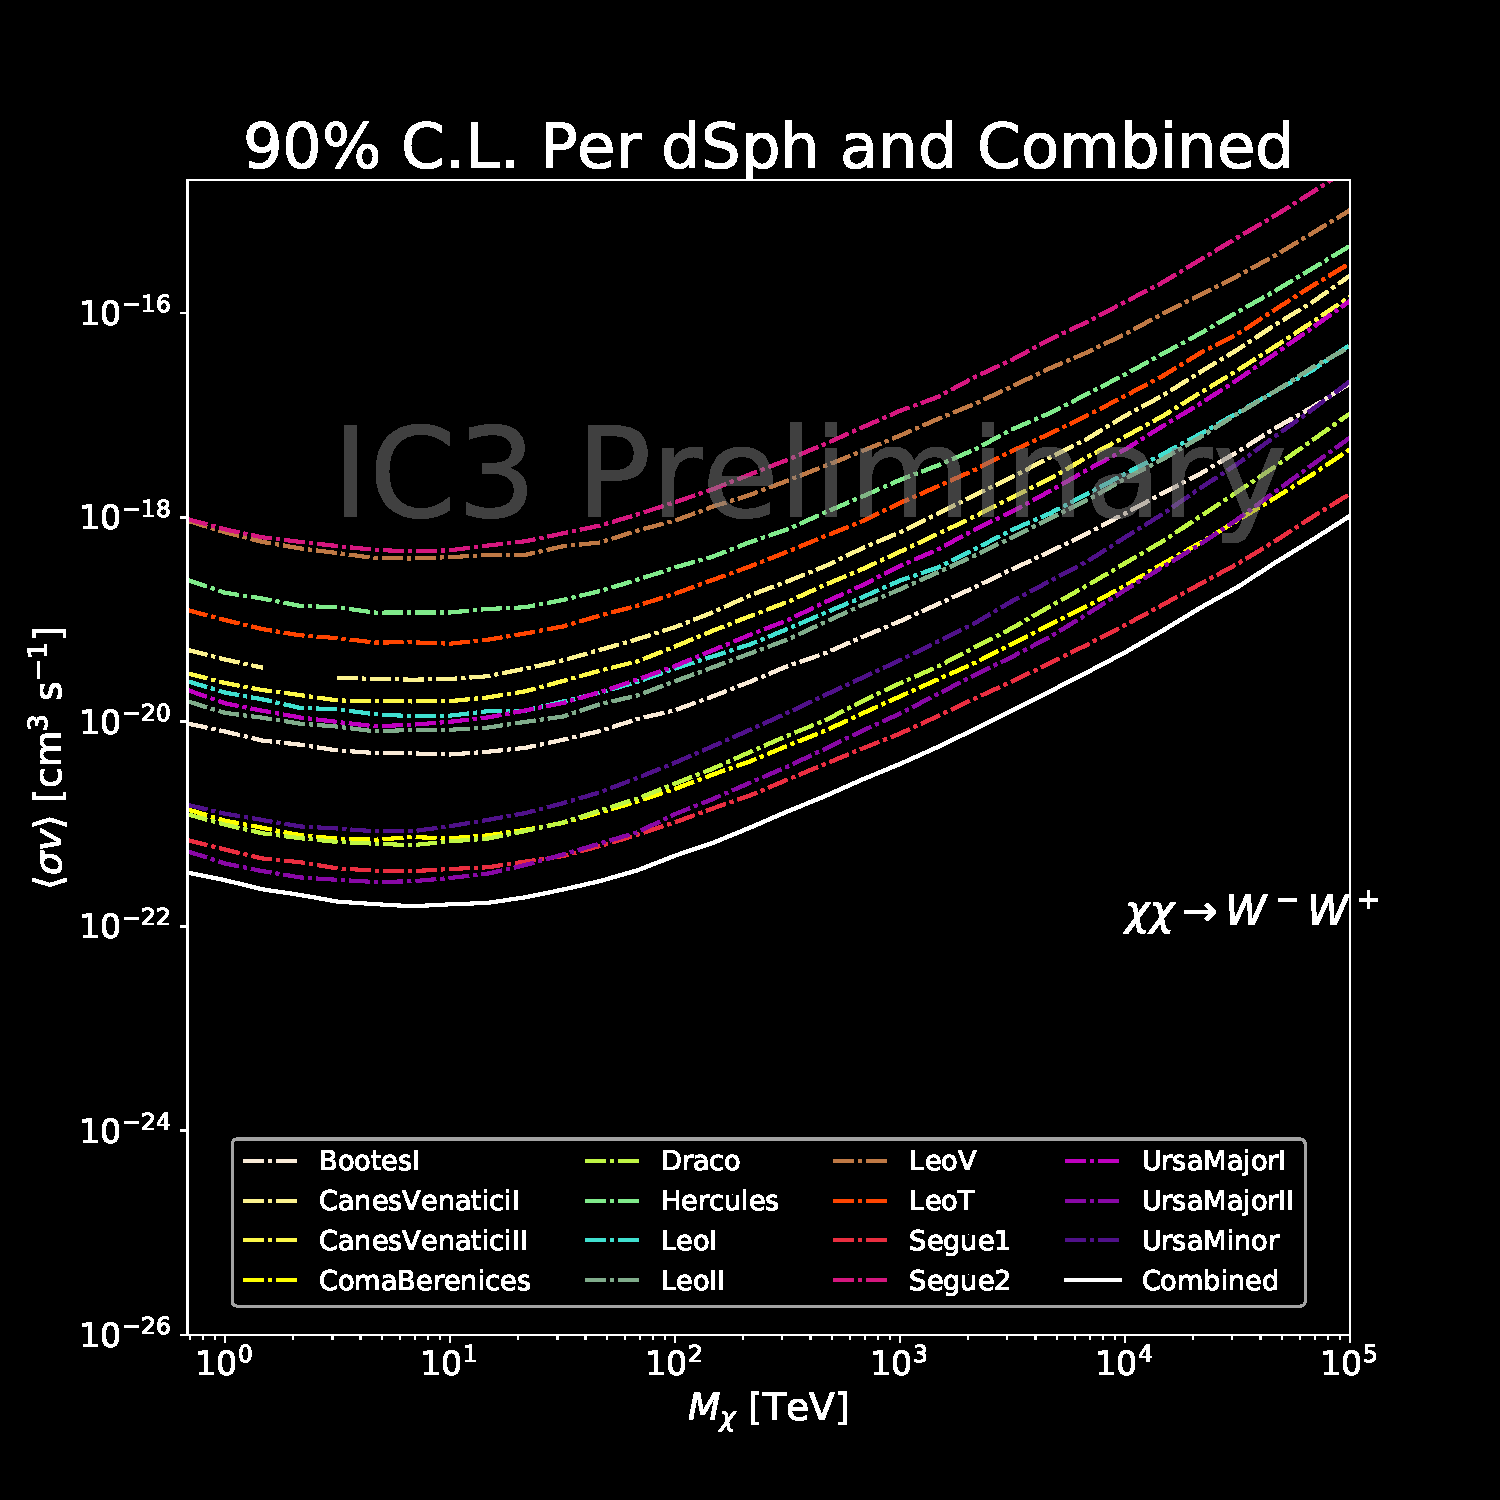
\includegraphics[scale=0.275]{figures/ic_DM/dm_plots/WW_money_plot_comb.pdf}
        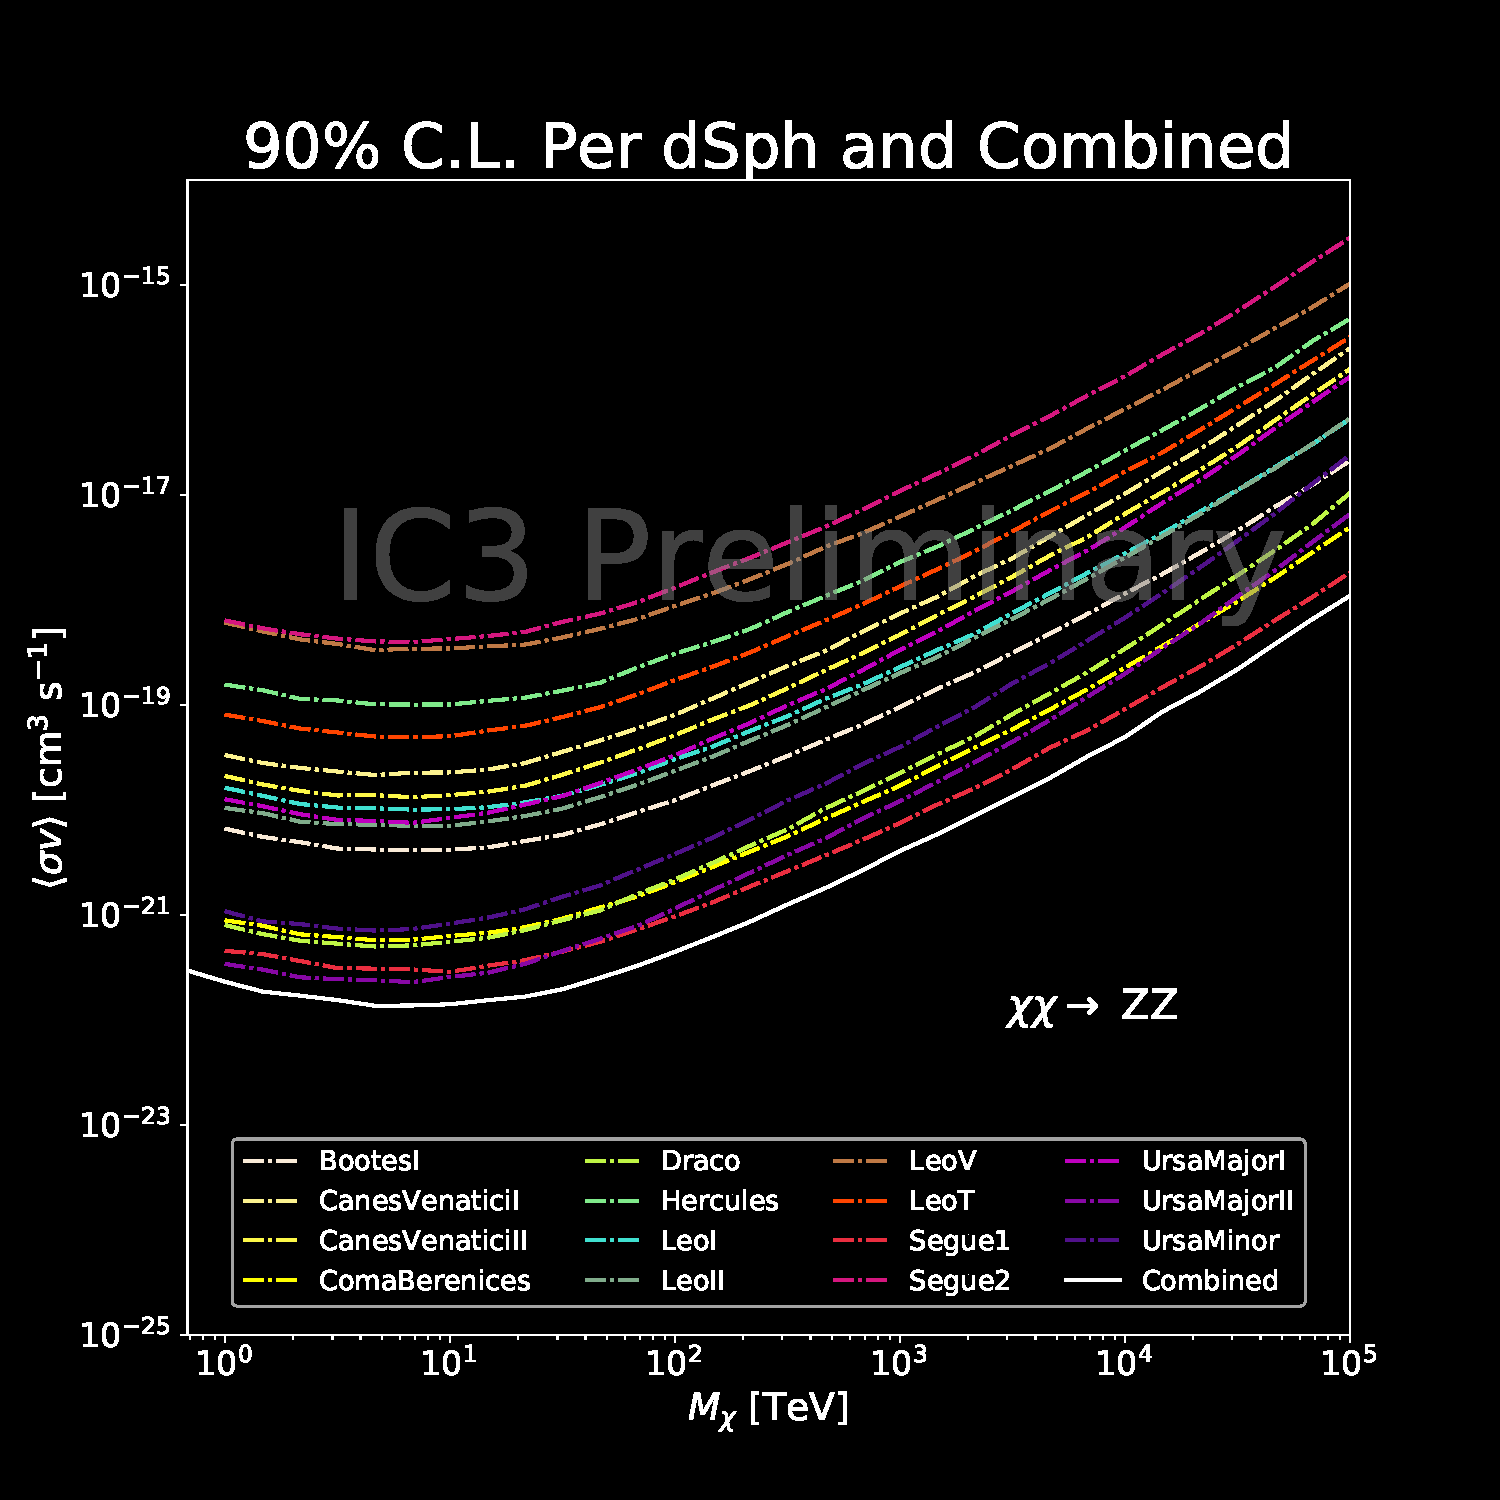
\includegraphics[scale=0.275]{figures/ic_DM/dm_plots/ZZ_money_plot_comb.pdf}
    }
    \caption{Words. I predent Icecibe Sensitivities weeee}
    \label{fig:icDM_sensitivity_1of2}
\end{figure}

\begin{figure}[b]
    \centering{
        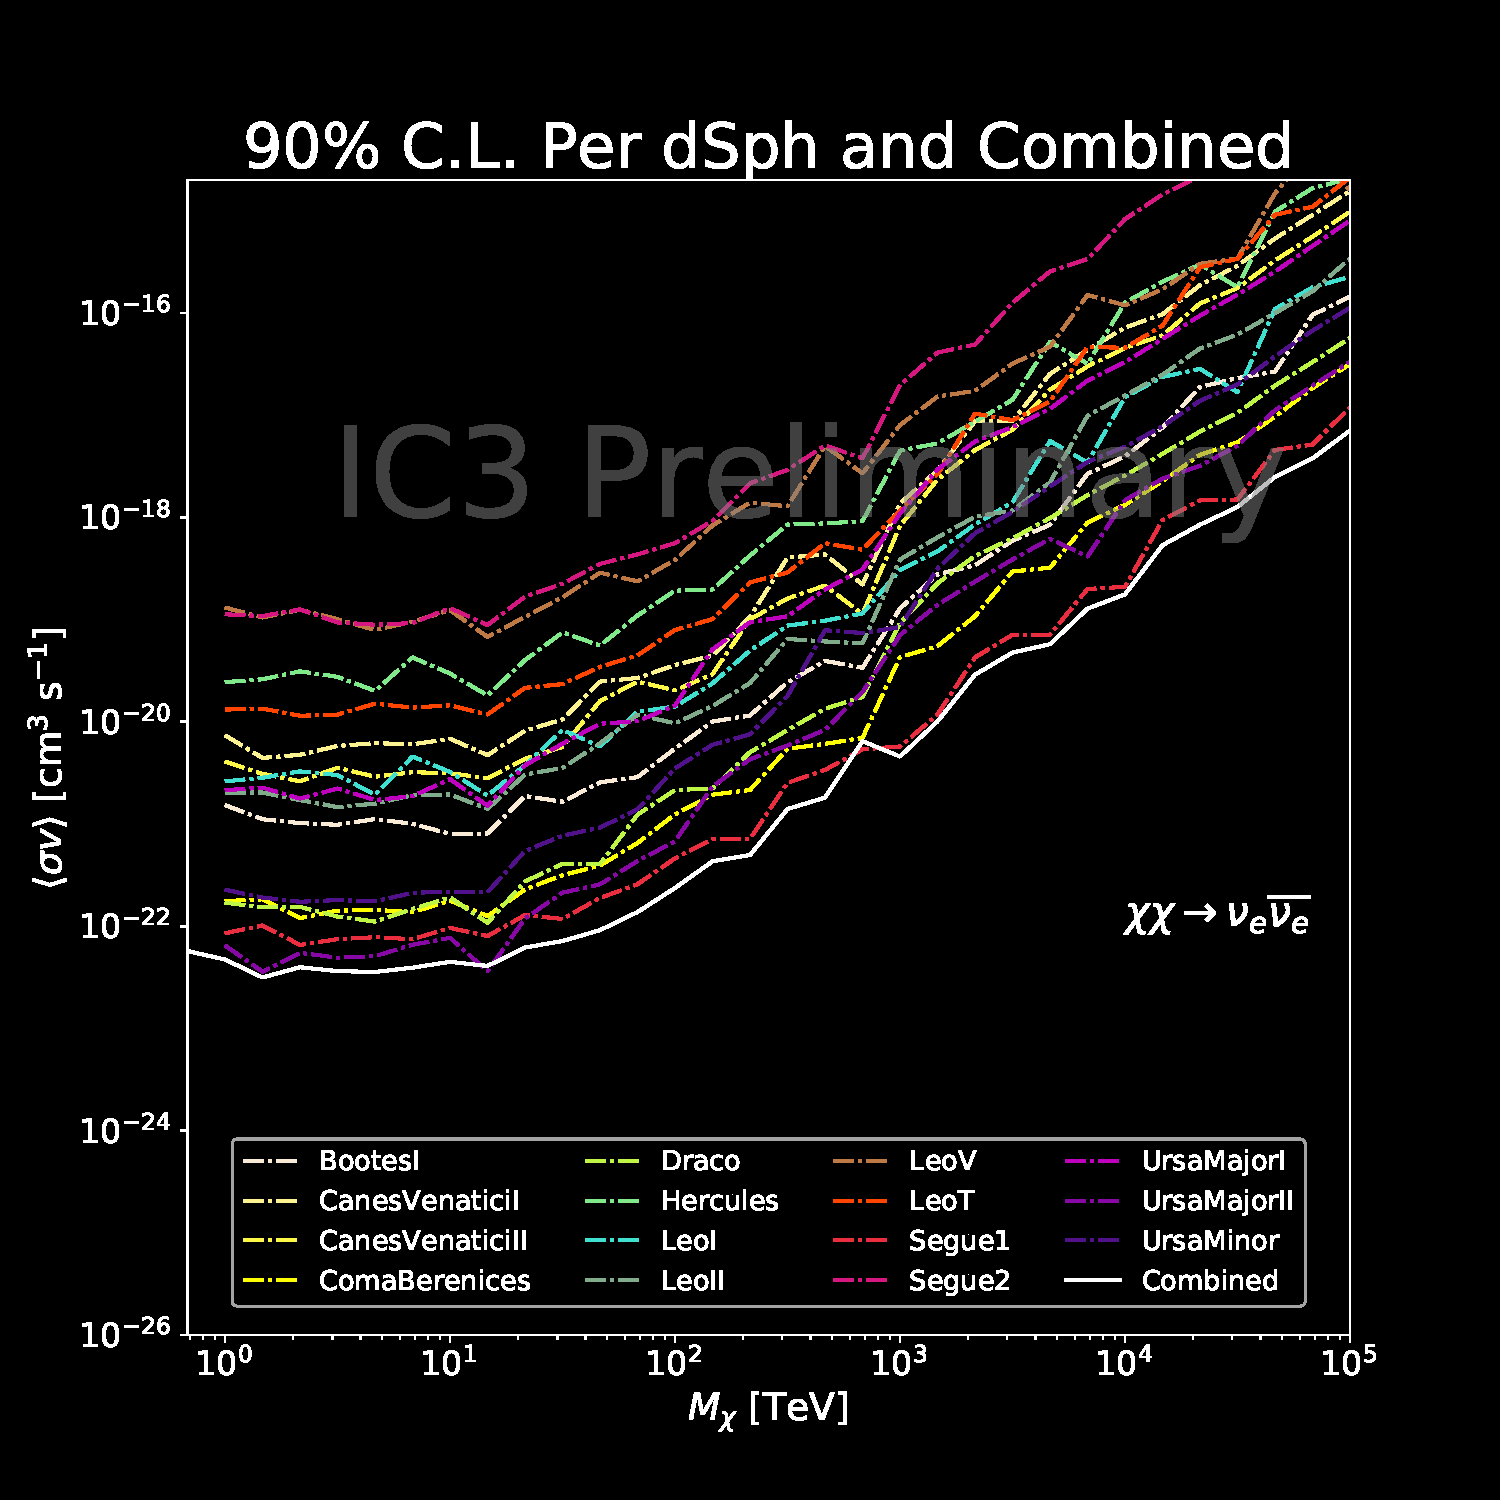
\includegraphics[scale=0.275]{figures/ic_DM/dm_plots/nuenue_money_plot_comb.pdf}
        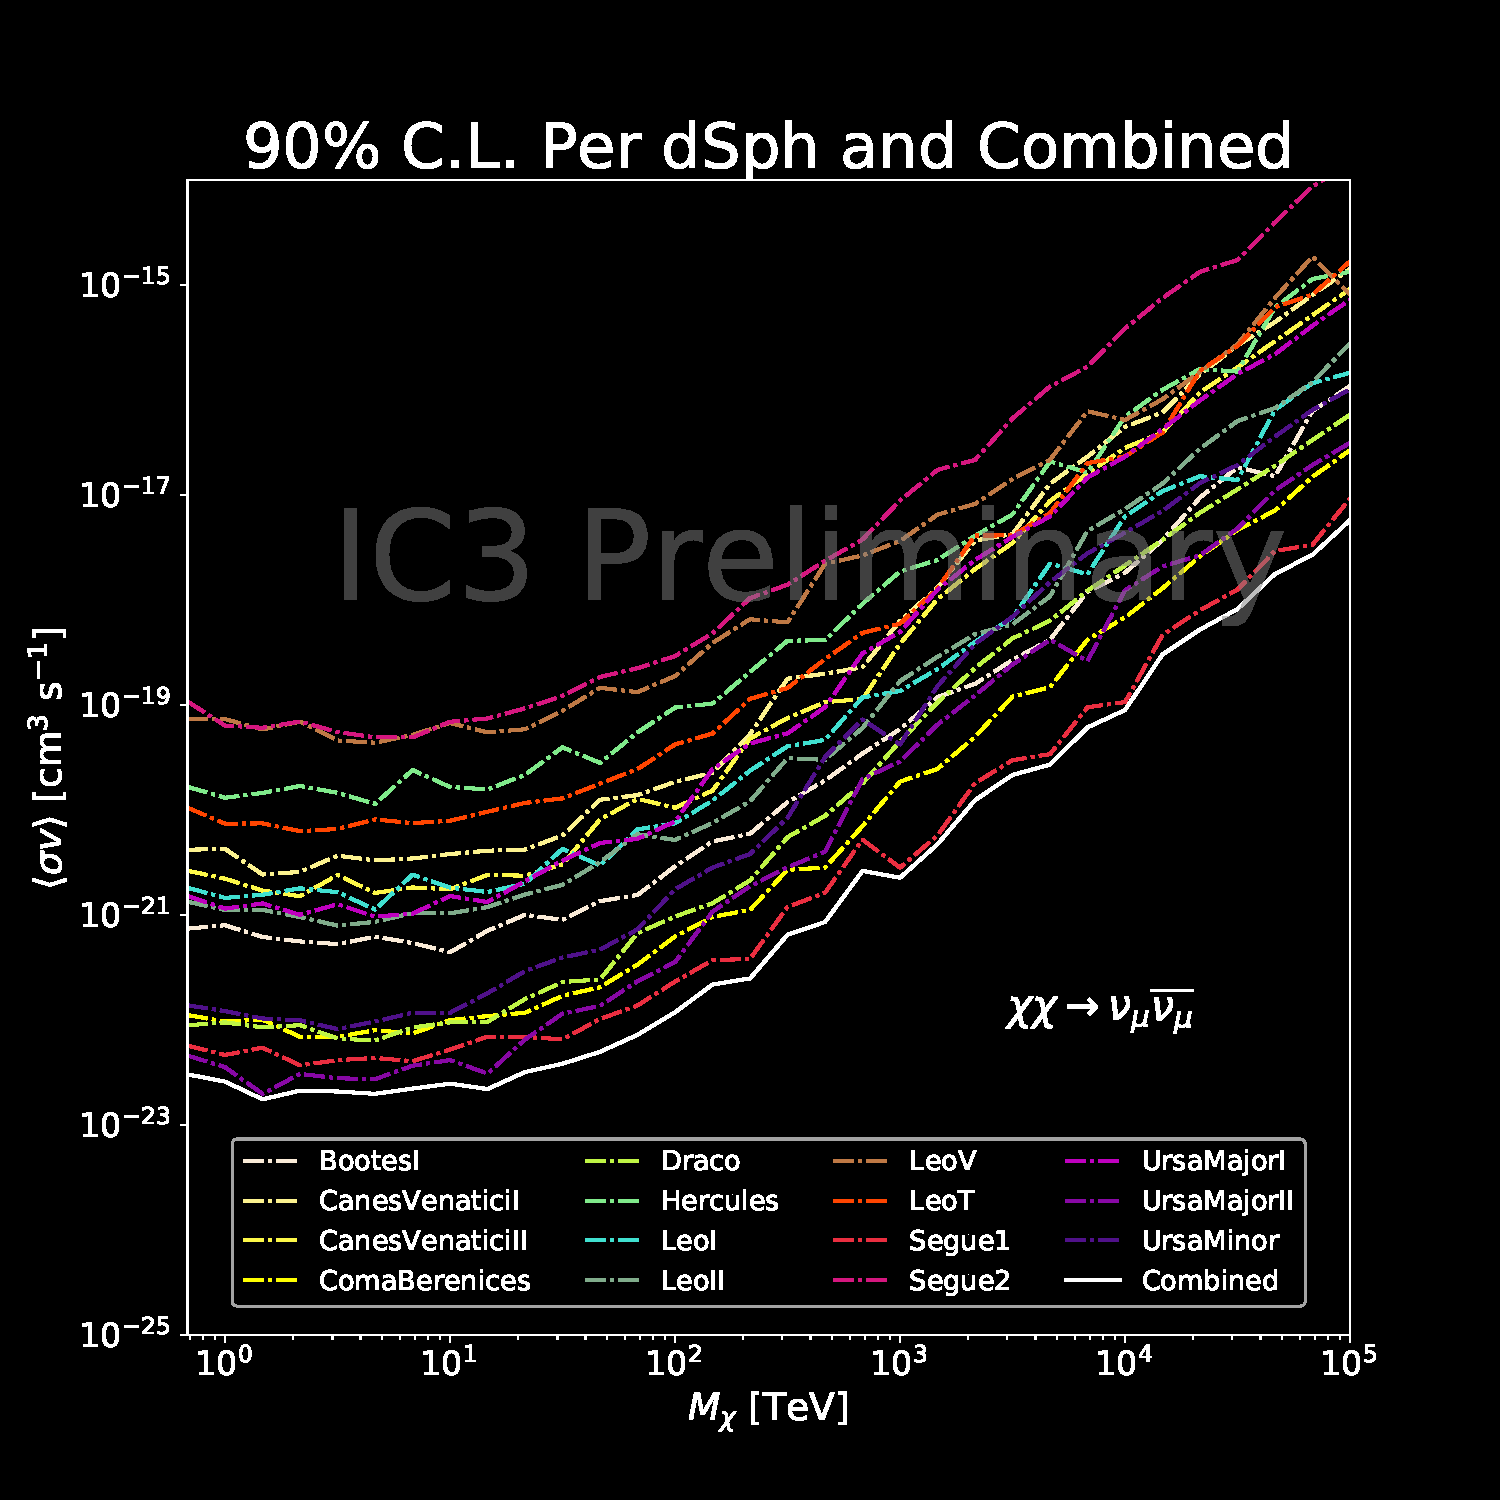
\includegraphics[scale=0.275]{figures/ic_DM/dm_plots/numunumu_money_plot_comb.pdf}
        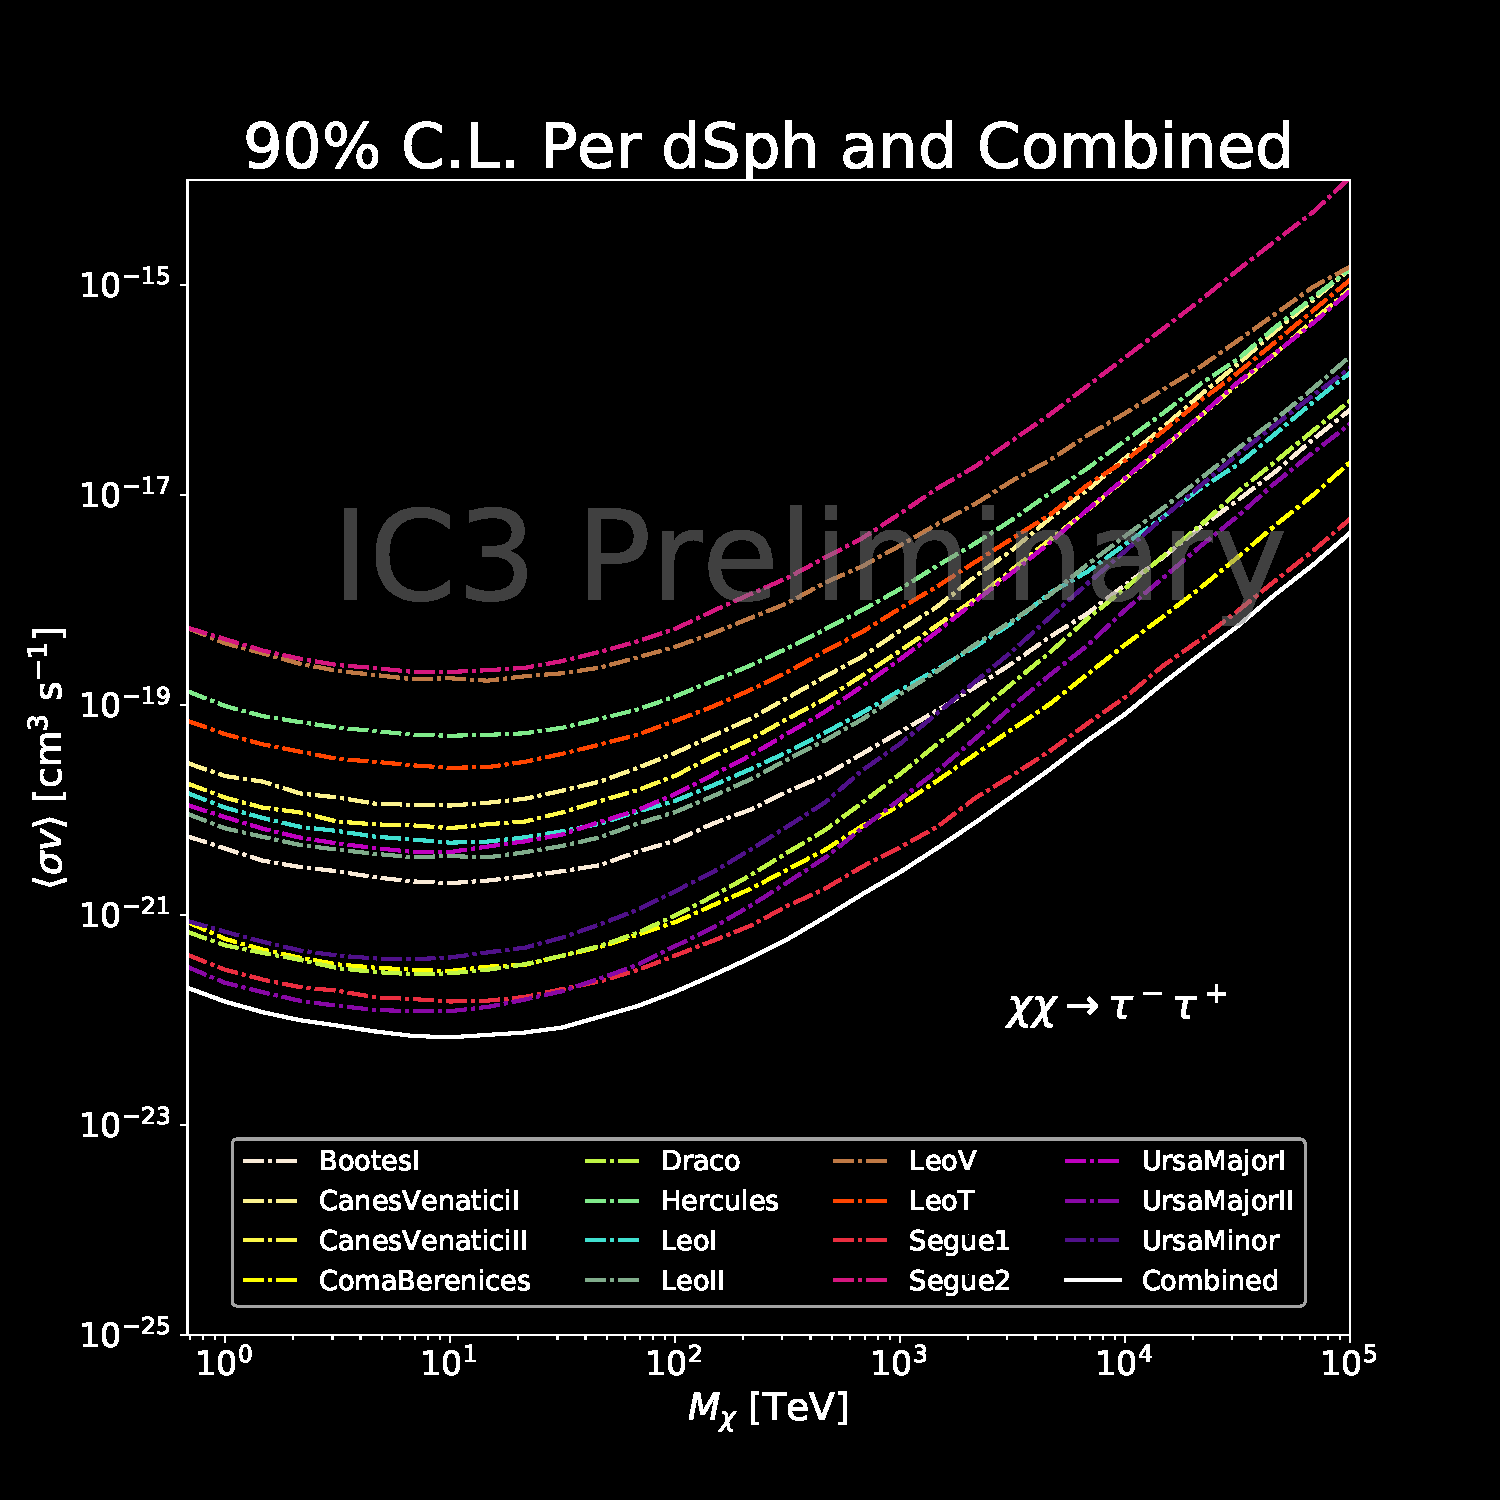
\includegraphics[scale=0.275]{figures/ic_DM/dm_plots/tautau_money_plot_comb.pdf}
    }
    \caption{Words. I predent Icecibe Sensitivities weeee}
    \label{fig:icDM_sensitivity_2of2}
\end{figure}
%%%%%%%%%%%%%%%%%%%%%%%%%%%%%%%%%%%%%%%%%%%%%%%%%%
\section{Systematics} \label{sec:icDM_Systematics}
%%%%%%%%%%%%%%%%%%%%%%%%%%%%%%%%%%%%%%%%%%%%%%%%%%

Lol What Systematics.
Beside signal recovery we don't have many additional studes for here.
The current analysis plan is to compare these sensitivities to another \J-factor catalog such as \LS \cite{DM_Strigari20}.
Additionally, we set out to perform a standard suite of IceCube systematic studies which include: \todo{THE BIG 4: ICE MODEL ETC}

%%%%%%%%%%%%%%%%%%%%%%%%%%%%%%%%%%%%%%%%%%%%%%%%%%
\section{Conclusions} \label{sec:icDM_conclude}
%%%%%%%%%%%%%%%%%%%%%%%%%%%%%%%%%%%%%%%%%%%%%%%%%%

We built many things for this analysis.
We utilized advanced computing techniques like parrallel programming and spline fitting of particle physics Monte Carlo to greatly expand and refine IceCube's sensitivity to DM annihilation from dSphs.
We imported updated astrophysical and particle physics models that better represent what we beleive neutrino signals from DM annihilation should look like.
We, for the first time, build an analysis that is sensitivty to PeV DM annihilation.

When we compare to previous IceCube publications of dSphs \cite{IC3_DM2013}, we see an order of magnitude imrovement to our sensitivity.
This analysis has been working group approved within IceCube and has begun the unblinding process.
This processes did not complete in time for this dissertation.
Therefor we do not show data for this thesis and is the clear next step.

The test statistic distributions in this analysis also demonstrate more characteristic behaviour compared to previous DM analyses.
With a 10 year dataset, we finally have enough statistics to almost trivially combine with other photon obervatories, such as HAWC.
The first ground work for a multi-messenger DM search is provided with concluding remarks in \cref{sec:nu_duck}.